\documentclass[11pt,doublespace]{unhthesis}

\includeonly{
sections/Introduction,
sections/SatelliteAttitudeModeling,
sections/TableSat1A,
sections/TableSatAttitudeDynamicsSoftware,
sections/StateError,
sections/Estimators,
sections/Controllers,
sections/ObserverBasedControls,
sections/SoftwareProgression,
sections/TSatPy,
sections/Conclusions,
sections/FutureWork,
sections/EquationSummary,
}

\usepackage{custom}
\hyphenation{gno-mon-ly}


\begin{document}

\title{Development of a Modular Application for Observer Based Control Systems for NASA's Spin-Stabilized MMS Mission Spacecraft}
\author{Daniel R. Couture}
\prevdegrees{B.S. Mechanical Engineering, University of New Hampshire, 2001}
\major{Mechanical Engineering}
\degree{Master of Science}
\degreemonth{May}
\degreeyear{2014}
\thesisdate{March 15, 2014}
\DOCUMENTtype{THESIS}
\Documenttype{Thesis}
\documenttype{thesis}
\maketitle

\copyrightyear{2014}
\makecopyright

\supervisor{Dr. May-Win L. Thein}{Associate Professor of Mechanical Engineering}
\committee{Dr. Barry Fussell}{Professor of Mechanical Engineering}
\committee{Philip J. Hatcher}{Professor of Computer Science}
\makeapproval

\begin{dedication}
  I would like to thank the people I would like to thank.
\end{dedication}

\begin{acknowledgments}
  TableSat1A: Johs Laakso, Jeff Kite, Dan Castelli, Michelle Pellitier, Ben Jenkins,
  \TODO{CS student}
  TableSat1B
  TableSat1C
    I would like to fin ack
\end{acknowledgments}

\begin{singlespace}
  \tableofcontents
  \addcontentsline{toc}{section}{LIST OF TABLES}
  \listoftables
  \addcontentsline{toc}{section}{LIST OF FIGURES}
  \listoffigures
\end{singlespace}

\begin{abstractpage}
This thesis utilizes an experimental table top satellite prototype (NASA MMS TableSat 1A) to span two main efforts.  The first is to create a physical model of a satellite for NASA's Magnetospheric MultiScale (MMS) Mission in order to validate and compare varied gyroless attitude determination and control systems (ADCS) techniques.  The ADCS maintains the TableSat constant 3 rpm rotation, prevents boom oscillations, and detects and corrects for unwanted nutation.  The second effort is a software system that can be used to implement theoretical and experimental models.  The system provides near ``real-time'' feedback of the system's states, and allows for ``on-the-fly'' modification to control parameters.  The system is specifically designed such that any control systems engineer is able to customize and extend its functionality without substantial programming expertise.
\end{abstractpage}




\chapter{Introduction}
\label{chap:Introduction}

\section{NASA Magnetospheric MultiScale Mission}
\label{sec:NASAMagnetosphericMultiScaleMission}

NASA's Magnetospheric MultiScale (MMS) Mission is a Solar Terrestrial probe mission scheduled for launch in October 2014 \cite{mms_website}.  The mission consists of four identical satellites orbiting the Earth in a constellation formation flight.  Construction of the satellites is occurring at NASA's Goddard Space Flight Center (GSFC) where they are being equipped to study the microphysics of magnetic reconnection events within the Earth's magnetic fields.

\begin{figure}[H]
\centerline{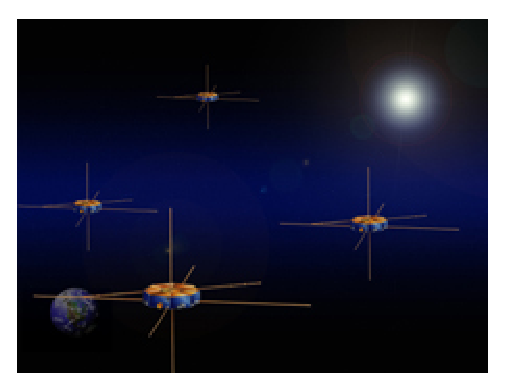
\psfig{file=figures/mms_spacecraft_formation.eps,height=1.2in}}
\caption{MMS Spacecraft Formation}
\label{fig:magneticfields}
\end{figure}

A reconnection event occurs when magnetic field lines cross allowing energetic particles to traverse from interstellar space into the Earth's magnetosphere releasing large quantities of heat and kinetic energy.  The diffusion region of a reconnection event starts on the day side magnetopause an quickly folds over to the Earth's magnetotail (Figure \ref{fig:magneticfields}).  This region is only 1-10 km in size but can travel at 10-100 km/hr \cite{swri} making it extremely difficult to measure.  Effects of a reconnection event are regularly experienced via the aurora borealis, interference with spacecraft GPS systems, and disruptions to electrical grids and communication networks.

\begin{figure}[H]
\centerline{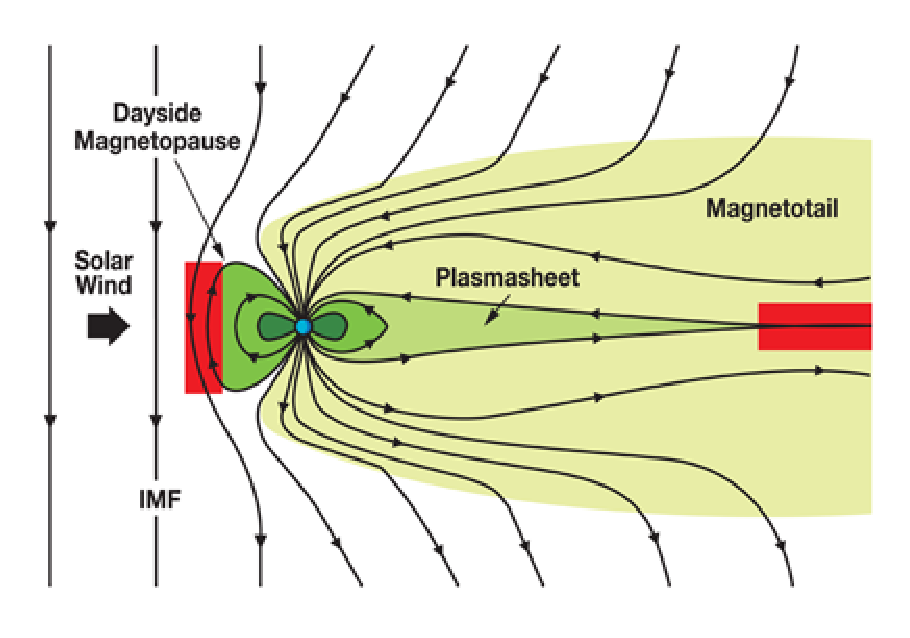
\psfig{file=figures/2d_earth_mag_field_lines.eps,height=1.2in}}
\caption{Earth's magnetic field}
\label{fig:magneticfields}
\end{figure}

Despite the widely experienced effects of reconnection events, very little about the microphysics inside its the diffusion region has been adequately measured.  Magnetometers, spectrometers, and other equipment currently in orbit are only able to capture a small fraction of the event's behavior.  Most equipment collect data from a single point or direction in space or some can get a 360 view of space by applying a slow spin to the spacecraft.  Both of these measurement methods are insufficient at capturing the structure of the diffusion region as it passes.

MMS's four satellites will be equipped with instrumentation mounted at the end of six boom extending out from the spacecraft's body along each major axis.  Four boom are the Spin Plane Double Probes (SDP) and two Axial Double Probes (ADP).  This configuration along with high resolution electron and ion spectrometers gives the constellation a new insight into the internal structure of the diffusion region.  The instrumentation at the ends of the boom are an advantage to the science portion of the mission, but create a unique challenge for the Attitude Determination and Control Systems (ADCS).  The satellites are spin stabilized at a rate of 3 rpm.  Disturbances to the rotation could translate into undesirable boom dynamics and nutations off the spin plane.



% Science questions to answer \cite{mms_website}
%     What determines when reconnection starts and how fast it proceeds?
%     What is the structure of the diffusion region?
%     How do the plasmas and magnetic fields disconnect and reconnect in the diffusion regions?
%     What role do the electrons play in facilitating reconnection?
%     What is the role of turbulence in the reconnection process?
%     How does reconnection lead to the acceleration of particles to high energies?


% \todo{image of formation flight}
% study microphysics of
%   magnetic reconnection
%   energetic particle acceleration
%   turbulence

% s/c MMS-1, MMS-2..MMS-4
% reconnection: Electromagnetic energy from the sun interacts with Earth's magnetosphere causing magnetic field lines to cross and create a burst of energy \cite{nasa_edge_video_ne_at_mms}
% magnetic reconnection measured ions and electrons as boundary passes to create 3d model of it passing by
% Fast plasma investigation
% probing the electron diffusion region (EDR) (passes too rapidly to get an accurate view with current equipment small (1-10 km) and rapidly moving (10-100 km/s))
% adjacent magnetic fields generally have significantly different orientations such that when they intersect, a large amount of energy is dispursed within a small region in the form of heat and kinetic energy.  The region = diffusion region
% explore magnetic reconnection
% dynamic regions of magnetosphere
% orbits planned to pass through the upstream and downstream magnetic reconnection sites
% 1) day side - solar wind field lines connection
% 2) down stream -
% 3) plasma travels down and causes the Arura
% through magnetospheric reconnection, portals allow energetic particles to traverse from outside to the interior of the magnetosphere
% predict when solar space weather within the magnetosphere and if they will affect orbiting satellites
% adverse space weather within the magnetosphere can negatively impact spacecraft system health GPS, induce disruptive current in electrical grids, communications, increased radiation exposure on trans-polar flights

% Difficult to understand
% magnetic boundary passes satellites quickly so has been hard to measure
% MMS has instruments to capture measurements
% Instruments mounted on all sides of the
% 8 sensors 1/30th sec instead of

% October 2014, Atlas five launch \cite{nasa_edge_video}

% Sensors
%   star sensor -> attitude
%   accelerometers -> $\Delta V$


% Fast Plasma Instrument (FPI) - controls
%   16 Dual Electron spectrometer (DES) Goddard built
%   16 Dual Ion Spectrometer (DIS) Japan *** built, hand delivered
%   180 degree and +- 22 degree measurement
%   30 millisec measurement rate 100x faster than previous missions entire view of sky
% FPI
%   despins data

% Instument Data processing Unit (IDPU) - brains of measurements
%   collects, compresses, transmits requested measurement data
%   configure while on mission

% booms
%   eight deployable booms
%   two 12.5m axial booms (electric field sensors)
%   four 60m wire booms
%   two 5m booms in spin plane for magnetometers
% rigid, wire, top/bottom booms
% important to keep consistent spin rate to get accurate estimates of boom location


% \section{Propulsion}

% types: solid propellents, bi propellents, electro propulsion, cold gas systems
% chose: mono-propellant blowdown - hydrozene power thrusters \cite{nasa_edge_video_propulsion}
% 3 rpm
% radial thrusters - spinning
% axial thrusters - prevent nutation

% concern:
% propulsion introduce distrubances

% 20 second pulses

% fuel limits by number of adjustments


% \section{performance requirements}

% $\pm 0.5$ deg attitude tollerance
% 1/10th of a second

\section{Research Objective}
\label{sec:ResearchObjective}

The work described in this thesis utilizes an experimental tabletop satellite (TableSat) \cite{vessthesis} to span three main efforts.  First is to create a physical model of a satellite from NASA's Magnetospheric MultiScale (MMS) Mission in order to validate and compare varied gyroless attitude determination and control (ADC) techniques.  The ADC systems must keep the TableSat rotating at a constant 3 rpm, prevent boom oscillations, and correct for detected nutations off the spin plane.  The second goal is to produce a software system that can be used to run against both theoretical simulations and experimental models.  The third goal is improve TableSat's use as an outreach tool.  The system should provide near ``real-time'' feedback of the system's state, allow for on-the-fly modification to control parameters, and be designed such that a individuals specializing in control systems could customize and extend its functionality without substantial computer science expertise.

\section{Past Work}
\label{sec:PastWork}

This work is a direct extension off of Vess' \cite{vessthesis} research using TableSat through Matlab Simulink and onboard flight controllers to demonstrate fundamentals of control theory.  The TableSat experimental design was modified to study the system dynamics of the instrument booms and nutation actuators in NASA's MMS mission satellites.  Previous experimental \cite{tsat1b} \cite{tsat1c} \cite{tsat2} and analytical \cite{mushawehthesis} ADC work at University of New Hampshire's Advanced Control Lab (ACL) has been done targeting the MMS mission.  The TableSat platform or similar derivations have also been adapted in investigate other areas of research including embedded systems development \cite{tablesat_xuml} and fault tolerant control \cite{tablesat_object_bench} \cite{nanjing_university}.


\section{Analytical and Experimental Testbed}
\label{sec:AnalyticalandExperimentalTestbed}



\section{Thesis Contributions}
\label{sec:ThesisContributions}

This research contributes to the field of feedback control, particularly as it relates to spin stabilized spacecraft, in the following ways:

\begin{itemize}
\item Gyroless observer-based controllers used to detect and eliminate nutations and maintain control of a spin stabilized satellite.
\item Improved capabilities of validating observer-based control methods by keeping identical control systems between analytical simulations and real experiments.
\item Allow clusters of estimators and controllers to all receive the same update for improved side-by-side comparisons of effectiveness.
\item Reduce time required to tune a controller by allowing for gain adjustments and swapping of estimation/control techniques on-the-fly.
\item Decompose quaternion state into separate rotational and nutation quaternions for use in error correction.
\item Use decomposed quaternion and differentiated rotational quaternions to decouple rate and attitude control.
\item Base quaternion state corrections on the representative rotational angle error, not the quaternion's sinusoidal scalar term.
\item Build the application such that the same control laws can be used to drive analytical simulations as well as experimental tests with physical systems.
\item Develop the application in a modular fashion to easily allow for future improvements and additions.
\item Control rates between modules such as sensors to estimators and estimators to controllers are independent and can operate at separate rates.
\item ``run-time'' feedback is available to visualize how the controller believes the system is responding.
\item A global clock instance is used for the authoritative time which during simulations can be adjusted in runtime to speed up or slow down the simulation to obtain better insight into the system dynamics.
\item Compensations for variable step sizes ($\delta t$) are made where able to protect the numerical integrity of the controller under large changes in control rates.
\item Code covered by proper software unit tests to validate and maintain expected behavior of the system during software upgrades.
\item Provide the combination of ``run-time'' visualizations and on-the-fly parameter/controller tuning for outreach programs.
\item Write the control application in a high level language to keep it accessible for improvements to control systems engineers with moderate programming experience.
\end{itemize}

\section{Thesis Outline}
\label{sec:ThesisOutline}




\chapter{SATELLITE ATTITUDE MODELING}
\label{chap:SatelliteAttitudeModeling}

This chapter will cover the analytical work behind in this thesis.  Starting with the choice of attitude and body rate representations in Section \ref{sec:StateRepresentation} and how the application was written to incorporate its use.  Next, a review of some of the estimation-based control methods used including variations on their use to target their use on spin-stabilized satellites such as NASA's MMS mission.  Then a summary of simulations run to validate the analytical model along with new tools used to visualize the system in ``run-time''.  Finally, testing of the analytical model against the physical system.

\section{State Representation}
\label{sec:StateRepresentation}

To represent the general state of a spin-stabilized satellite, are often accomplished using one of two representations.  Either body rates with Euler angles or body rates with quaternions with Euler angles being slightly more common among control theory specialists and quaternions used more in the implementation of the control systems.  Euler angles with rigid body dynamics and quaternions were chosen for the state representation.  Quaternions provided unique advantages over Euler angles that will be expanded on in Sections \ref{subsec:BodyRate} and \ref{subsec:QuaternionAttitude}.

\subsection{Body Rates}
\label{subsec:BodyRate}

NASA's MMS satellites as with all real systems are rarely linear.  When modeling the dynamics of a system with nonlinearities, a common first pass is to linearize the model and assume that the nonlinearities are either negligible or can be lumped in to system disturbances.  This approach was also taken here.  The two portions of the system's dynamics are loosely generalized into either the rigid body dynamics of the satellite's main or the flexible dynamics of the attached booms.  Kaplan \cite{kaplan} covers the creation of the rigid body Euler's moment equations.

\begin{subequations}
  \begin{align}
    M_x = \dot{h}_x + \omega_y h_z - \omega_z h_y \\
    M_y = \dot{h}_y + \omega_z h_x - \omega_x h_z \\
    M_z = \dot{h}_z + \omega_x h_y - \omega_y h_x
  \end{align}
  \label{eqn:EulerMoment}
\end{subequations}

Here the equations of motion are described in terms of the body's frame of reference ($x$, $y$, $z$) which does not necessarily align with the body's principal axes.  TableSat 1A's construction can be simplified to an axisymmetric design.  To adjust TableSat 1A's stability, the center screw can be raised or lowered bringing the center of mass and center of rotation closer or further apart.  As development of the observer-based controller improves the two centers can be brought closer together.  With these conditions, we can assume that the body's reference frame aligns with the body's principal axes, which simplifies Euler's equations further to.

\begin{subequations}
  \begin{align}
    M_1 & = I_1 \dot{\omega}_1 + \omega_2 \omega_3 (I_3 - I_2) \\
    M_2 & = I_2 \dot{\omega}_2 + \omega_1 \omega_3 (I_1 - I_3) \\
    M_3 & = I_3 \dot{\omega}_3 + \omega_1 \omega_2 (I_2 - I_1)
  \end{align}
  \label{eqn:EulerMomentPrincipleAxes}
\end{subequations}

For implementation into the TableSat 1A's base station observer based controller, the continuous time Euler's equations \ref{eqn:EulerMomentPrincipleAxes} get converted to discrete time with a variable time step and implemented in Appendix \ref{code:TSatPy/State.py} as

\begin{subequations}
  \begin{align}
    \dot{\omega}_{x}(t_{k+1}) & = \frac{1}{I_x} \left[ M_1(t_{k+1}) - (I_z - I_y) \omega_{y}(t_k) \omega_{z}(t_k) \right] \\
    \dot{\omega}_{y}(t_{k+1}) & = \frac{1}{I_y} \left[ M_2(t_{k+1}) - (I_x - I_z) \omega_{x}(t_k) \omega_{z}(t_k) \right] \\
    \dot{\omega}_{z}(t_{k+1}) & = \frac{1}{I_z} \left[ M_3(t_{k+1}) - (I_y - I_x) \omega_{x}(t_k) \omega_{y}(t_k) \right]
  \end{align}
  \label{eqn:DiscreteEulerMomentEquations}
\end{subequations}

The moments $M_n(t_{k+1})$ are the applied moments at time $t_{k+1}$.  Since the update frequencies are allowed to vary for each section of the observer-based controller, the applied moment values may have multiple values between $t_{k}$ and $t_{k+1}$.  To avoid the complexity of calculating a more accurate moment for each time step that is a combination of changes in applied moments, the value of the most recent moments is taken and assumed constant for $t_{k} < t < t_{k+1}$.  If the moment update loop is running slower than the Euler equation model, the last known moment is assumed to still be valid.

While the Euler equation model works well for propagating the state of the system's, Section \ref{sec:Sensors} found that the only sources of state measurement were in attitude leaving body rates unmeasured.  Body rates must then be calculated through both observing changes in current attitude and state predictions based on previous attitude changes.  Euler angles and quaternions were investigated for parameterizing TableSat's attitude.

Euler angles were first considered because of their wide use in control theory where the representation of a body's attitude can be reached through a series of no more than three roll, pitch, yaw rotations.   Out of the twelve possible sequences, the 3-1-3 sequence is commonly used in spacecraft ADCS.  With this sequence Kaplan \cite{kaplan}, shows that the conversion between Euler angle rates and body rates can be calculated with

\begin{equation}
  \begin{bmatrix}
    \omega_x \\
    \omega_y \\
    \omega_z \\
  \end{bmatrix}
  =
  \begin{bmatrix}
    \sin \theta \sin \phi & \cos \phi & 0 \\
    \sin \theta \cos \phi & - \sin \phi & 0 \\
    \cos \theta & 0 & 1 \\
  \end{bmatrix}
  \begin{bmatrix}
    \dot{\psi} \\
    \dot{\theta} \\
    \dot{\phi} \\
  \end{bmatrix}
  \label{eqn:EulerToBodyRate}
\end{equation}

Euler angles while widely used and for most people easier to visualize, they have two main deficiencies.  They are heavily reliant on trigonometric functions and under certain conditions can cause singularities as seen by transforming Equation \ref{eqn:EulerToBodyRate} to solve for the Euler rates where a $1/\sin \theta$ factors out (Equation \ref{eqn:BodyRateToEuler}.  This phenomenon is more generally known as gimbal lock.  The second deficiency occurs in implementation, where the efficiency and stability of the angles are tied to the accuracy of trigonometric approximations in the code's library.  These repeated approximations are more prone to numerical drift.

\begin{equation}
  \begin{bmatrix}
    \dot{\psi} \\
    \dot{\theta} \\
    \dot{\phi} \\
  \end{bmatrix}
  =
  \frac{1}{\sin \theta}
  \begin{bmatrix}
    \sin \phi & \cos \phi & 0 \\
    \cos \phi \sin \theta & -\sin \phi \sin \theta & 0 \\
    -\sin \phi \cos \theta & -\cos \phi \cos \theta & \sin \theta \\
  \end{bmatrix}
  \begin{bmatrix}
    \omega_x \\
    \omega_y \\
    \omega_z \\
  \end{bmatrix}
  \label{eqn:BodyRateToEuler}
\end{equation}

The alternative attitude parameterization investigated was the quaternion attitude representation the conversion from body discrete body rates to quaternion attitude is calculated via the method from Trawny and Roumeliotis at the University of Minnesota \cite{marslab}.

\begin{equation}
  \begin{aligned}
    \bs{q}(t_{k+1}) = & \bigg[ \exp \left( \frac{\Delta t_{k+1}}{2} \bs{\Omega} \left[ \bs{\bar{\omega}}(t_{k+1}) \right] \right) + \\
    & \frac{1}{48} \Delta t_{k+1}^2 \Big(
    \bs{\Omega} \left[\bs{\omega}(t_{k+1}) \right]
    \bs{\Omega} \left[\bs{\omega}(t_{k})   \right] -
    \bs{\Omega} \left[\bs{\omega}(t_{k})   \right]
    \bs{\Omega} \left[\bs{\omega}(t_{k+1}) \right]
      \Big) \bigg] \bs{q}(t_{k})
  \end{aligned}
  \label{eqn:DiscreteQuaternionPropagation}
\end{equation}

where

\begin{equation}
    \bs{\Omega} \left[ \bs{\bar{\omega}}(t_{k+1}) \right] = \frac{\bs{\Omega} \left[\bs{\omega}(t_{k+1}) \right] + \bs{\Omega} \left[\bs{\omega}(t_{k}) \right]}{2}
    \label{eqn:DiscreteQuaternionToBodyRate}
\end{equation}

\begin{equation}
  \bs{\Omega} \left[ \bs{\omega} \right] =
  \begin{bmatrix}
    - [ \bs{\omega} \times ] & \bs{\omega} \\
    - \bs{\omega}^T & 0 \\
  \end{bmatrix}
  \label{eqn:OmegaMatrix}
\end{equation}

\begin{equation}
  \bs{\omega} \times =
  \begin{bmatrix}
    0 & -\bs{\omega}_z & \bs{\omega}_y \\
    \bs{\omega}_z & 0 & -\bs{\omega}_x \\
    -\bs{\omega}_y & \bs{\omega}_x & 0 \\
  \end{bmatrix}
\end{equation}


\subsection{Quaternion Attitude}
\label{subsec:QuaternionAttitude}

The concept of a quaternion is a combination of geometry and algebra based focus from Rodrigues and Hamilton respectively \cite{shuster}.  Rodrigues' work in the early 1800's focused the Gibbs vector as a way of creating a an attitude matrix from the Rodrigues parameters.  Hamilton's work focused on hyper-complex numbers with three hyper-imaginary values and a constant.  Hamilton first coined the term quaternion in 1843 to describe the four dimensional vector.  The four orthogonal unit quaternions are

\begin{subequations}
  \begin{align}
    \bs{1} = & 1 + 0\bs{i} + 0\bs{j} + 0\bs{k} \\
    \bs{i} = & 0 + 1\bs{i} + 0\bs{j} + 0\bs{k} \\
    \bs{j} = & 0 + 0\bs{i} + 1\bs{j} + 0\bs{k} \\
    \bs{k} = & 0 + 0\bs{i} + 0\bs{j} + 1\bs{k}
  \end{align}
  \label{eqn:UnitQuaternions}
\end{subequations}

where the unit quaternions obey Hamilton's rules \cite{wolfram_quaternion}

\begin{subequations}
  \begin{align}
    \bs{i}^2 = \bs{j}^2 = \bs{k}^2 = \bs{ijk} & = - \bs{1} \\
    \bs{i}\bs{j} = -\bs{j}\bs{i} &= \bs{k} \\
    \bs{j}\bs{k} = -\bs{k}\bs{j} &= \bs{i} \\
    \bs{k}\bs{i} = -\bs{i}\bs{k} &= \bs{j}
  \end{align}
  \label{eqn:HamiltonRules}
\end{subequations}

As discussed in Section \ref{subsec:StateMeasurement}, between TableSat sensor and MMS mission restrictions, the body rate for this research is not measured.  This meant that the choice in attitude parameterization and how it is implemented play a major factor in the entire system's performance.  Because of their numerical stability and that over time I found working with quaternions more intuitive than Euler angles, the quaternion was chosen as the method for representing state attitude parameters.  From sections \TODO{label these later} to \TODO{XXX}, quaternion properties will be discussed along with how they were represented in the controller's implementation.

\subsubsection{Quaternion Notation}
\label{subsubsec:QuaternionNotation}

One point of confusion when working with quaternions is the placement of the scalar term.  As shown in Equation \ref{eqn:UnitQuaternions} the scalar term is followed by the three complex terms.  To stay consistent with related research, the quaternion notation to be used in this thesis follows the structure of 4 dimensional vector where the scalar term follows the vector.

\begin{equation}
  \bs{q} = \bs{v} + q_0 = q_1 \bs{i} + q_2 \bs{j} + q_3 \bs{k} + q_0
\end{equation}

In academic literature, the difference is not terribly significant as the notation is generally defined by the author or the reader can recognize the variation in structure.  For example in Equation \ref{eqn:OmegaMatrix}, written in a scalar last format, is composed from a 3x3, 3x1, 1x3, and 1x1.  During implementation, mixing of scalar first matrices with scalar last matrices can be a troublesome source of error.

\subsubsection{Rotational Quaternion}
\label{subsubsec:RotationalQuaternion}

Euler's rotation theorem states:

\begin{quote}{``\textsl{If $\bs{R}$ is a 3x3 orthogonal matrix $( \bs{R}^T \bs{R} = \bs{R}\bs{R}^T = \bs{I} )$ and $\bs{R}$ is proper $( det \bs{R} = +1 )$, then there is a nonzero vector $\bs{v}$ satisfying $\bs{Rv} = \bs{v}$}''~\cite{euler_theorem}}\end{quote}

With a 3x3 rotational matrix, this means there is a line of points that do not change position and create an axis of rotation.  Incorporating this idea into any spin-stabilized satellite like NASA's MMS mission yields that any arbitrary attitude can be represented as a single rotation from a common starting orientation.  The axis $\hat{e}$ and the angle of rotation $\theta$ can express the satellite's attitude with a rotational quaternion as

\begin{equation}
  \bs{q} = \bs{v} + q_0 = \hat{\bs{e}} \sin \left( \frac{-\theta}{2} \right) + \cos \left( \frac{-\theta}{2} \right)
  \label{eqn:RotationalQuaternionDefinition}
\end{equation}

A $-\theta$ is used rather than a the positive value to represents points on the body frame rotating around fixed axes rather than an axes transformation.  This representation also reduces the degrees of freedom for a quaternion from four to three as a rotational quaternion is restricted to always having a unit norm.

\begin{equation}
  \left| \hat{\bs{e}} \sin \left( \frac{-\theta}{2} \right) + \cos \left( \frac{-\theta}{2} \right) \right| = \left| \hat{\bs{e}} \right|  \sin^2 \left( \frac{-\theta}{2} \right) + \cos^2 \left( \frac{-\theta}{2} \right) = 1
\end{equation}

\subsubsection{Quaternion Multiplication}
\label{subsubsec:QuaternionMultiplication}

The quaternion multiplication noted with the infix operator $\otimes$, is the keystone to the attitude state manipulation and is used to produce incremental changes in the satellite's attitude.  If $\bs{a}$ represents a $n$ degree rotation about axis $\hat{e}$, then a $4n$ degree rotation about axis $\hat{e}$ can be represented as $\bs{a} \otimes \bs{a} \otimes \bs{a} \otimes \bs{a}$.

Let two quaternions $\bs{a}$ and $\bs{b}$ be represented as

\begin{subequations}
\begin{align}
  \bs{a} = \bs{a}_v + a_0 = & a_1 \bs{i} + a_2 \bs{j} + a_3 \bs{k} + a_0\\
  \bs{b} = \bs{b}_v + b_0 = & b_1 \bs{i} + b_2 \bs{j} + b_3 \bs{k} + b_0
\end{align}
\end{subequations}

The quaternion multiplication is defined as

\begin{equation}
  \bs{q} = \bs{a} \otimes \bs{b} = \bs{a}_v b_0 + \bs{b}_v a_0 + \bs{a}_v \times \bs{b}_v + a_0 b_0 - \bs{a}_v \cdot \bs{b}_v
  \label{eqn:QuaternionMultiplication}
\end{equation}

Expanding Equation \ref{eqn:QuaternionMultiplication} yields

\begin{subequations}
\begin{align}
  \bs{v} & = \begin{bmatrix} a_1 \\ a_2 \\ a_3 \end{bmatrix} b_0 +\begin{bmatrix} b_1 \\ b_2 \\ b_3 \end{bmatrix} a_0 + \begin{bmatrix} a_1 \\ a_2 \\ a_3 \end{bmatrix} \times \begin{bmatrix} b_1 \\ b_2 \\ b_3 \end{bmatrix} \\
  q_0 & = a_0 b_0 - \bs{a}_v \cdot \bs{b}_v
\end{align}
\end{subequations}

Evaluating the cross and dot products

\begin{subequations}
\begin{align}
  \bs{v} & = \begin{bmatrix} a_1 \\ a_2 \\ a_3 \end{bmatrix} b_0 +\begin{bmatrix} b_1 \\ b_2 \\ b_3 \end{bmatrix} a_0 + \begin{bmatrix} a_2b_3 - a_3b_2 \\ a_3b_1 - a_1b_3 \\ a_1b_2 - a_2b_1 \\ \end{bmatrix} \\
  q_0 & = a_0 b_0 - (a_1b_1 + a_2b_2 + a_3b_3)
\end{align}
\end{subequations}

\begin{subequations}
\begin{align}
  \bs{v} & = \begin{bmatrix} a_1b_0 + b_1a_0 + a_2b_3 - a_3b_2 \\ a_2b_0 + b_2a_0 + a_3b_1 - a_1b_3 \\ a_3b_0 + b_3a_0 + a_1b_2 - a_2b_1 \\ \end{bmatrix} \\
  q_0 & = a_0 b_0 - a_1b_1 - a_2b_2 - a_3b_3
\end{align}
\end{subequations}

Combining equations and factoring out the $b$ terms yields

\begin{equation}
  \begin{bmatrix} \bs{v} \\ q_0 \end{bmatrix} =
  \begin{bmatrix}
    a_0 & - a_3 &   a_2 & a_1 \\
    a_3 &   a_0 & - a_1 & a_2 \\
  - a_2 &   a_1 &   a_0 & a_3 \\
  - a_1 & - a_2 & - a_3 & a_0
  \end{bmatrix}
  \begin{bmatrix}
  b_1 \\ b_2 \\ b_3 \\ b_0
  \end{bmatrix}
\end{equation}

From here, the square matrix can be decomposed into sections based on if they get combined with quaternion $b$'s vector or scalar components.  Once segmented, the components of the square matrix can be expressed more compactly and in a way that conveys a better sense of how the quaternions interact on multiplication.

\begin{equation}
  \begin{bmatrix} \bs{v} \\ q_0 \end{bmatrix} =
  \begin{bmatrix}
    (\bs{a}_v \times) + \bs{I} a_0 & \bs{a}_v \\
    -\bs{a}_v^T                    & a_0 \\
  \end{bmatrix}
  \begin{bmatrix}
  \bs{b}_v \\ b_0
  \end{bmatrix}
  \label{eqn:QuaternionMultiplicationDerived}
\end{equation}

This quaternion class for TSatPy as will be covered in Chapter \ref{chap:TSatPy} allows for the a very close representation of Equation \ref{eqn:QuaternionMultiplicationDerived}.

% The advantage to this notation is that is much easier to run in a Numerical Simulation Software (NSS like Matlab or Octave) or other scripting language, but its layout is specific to our definition of the matrix where the scalar value follows the vector.  There is not clear consensus from the broader community on whether the vector or scalar should come first.  This can cause large issues when implementing a system using a externally provided library since both implementations expect a 4x4 matrix, and combining the logic from the two systems would require either rewriting of systems or spending extra cycles on the interface between the two systems converting the matrices from a scalar first to a scalar last layout and vice versa.

% The object oriented nature of the code written for this thesis reduces or eliminates the confusion.  When an instance of a quaternion class is created, the vector and scalar values are set as separate parameters on the object regardless of order.  So when used in computation the $\Re^3$ and $\Re^1$ values can be referenced directly through the vector and scalar properties respectively.  Chapter \ref{ch:object_oriented} will cover the structure of the code developed for the thesis in greater detail.  The specific code that governs interactions between quaternions in the model is in section \ref{code:lib/@quaternion/quaternion.m}.


\subsubsection{Rotating a Point with Quaternions}
\label{subsubsec:RotatingaPointwithQuaternions}

One of the main focal points of this thesis is to make sure the tools developed aide in outreach and demonstration.  To enable this goal, ``run-time'' analysis of the system is a key deliverable.  Waiting for a simulation to complete or a experimental run with TableSat before being able to access the information is not only an impedance to this end, but it also introduces complexity and higher ``run-time'' costs to collect and store the full history of the system for replay.  One advantage to having access to the system's parameters as the experiment proceeds is to be able to represent the inner workings of the algorithms for inspection.  In the case of an estimator, sensor voltages are converted to a measured state and the estimator attempts to guess the true state of the system.  A visualization of what the estimator thinks the TableSat is doing can run alongside the physical systems and the convergence between estimated and actual states can be readily observed.

To facilitate this, visualization a model of the TableSat can be rotated with a rotation matrix based on the estimated state's quaternion.  The 3x3 rotation matrix is defined as a function of a rotational quaternion by

\begin{equation}
  \bs{R_q} = (q_0^2 - \bs{v}^T \bs{v}) \bs{I} + 2 \bs{v} \bs{v}^T - 2 q_0 (\bs{v} \times)
  \label{eqn:RotationMatrix}
\end{equation}

For a $\pi/2$ radian rotation about $\hat{e} = 0\bs{i}+0\bs{j}+1\bs{k}$, the rotational quaternion an defined in Equation \ref{eqn:RotationalQuaternionDefinition} becomes $q = 0\bs{i}+0\bs{j}-1/\sqrt{2}\bs{k}+1/\sqrt{2}$.  With Equation \ref{eqn:RotationMatrix}, the rotational matrix becomes

\begin{equation}
  \begin{aligned}
    \bs{R_q} & = \left[ (1/\sqrt{2})^2 - (1/\sqrt{2})^2 \right] \bs{I} + 2 \begin{bmatrix} 0 & 0 & 0 \\ 0 & 0 & 0 \\ 0 & 0 & 1/\sqrt{2} \end{bmatrix} - 2 \frac{1}{\sqrt{2}} \begin{bmatrix} 0 & 1/\sqrt{2} & 0 \\ -1/\sqrt{2} & 0 & 0 \\ 0 & 0 & 0 \\ \end{bmatrix} \\
      & = \begin{bmatrix} 0 & -1 & 0 \\ 1 & 0 & 0 \\ 0 & 0 & 1 \\\end{bmatrix}
  \end{aligned}
\end{equation}

For the visualization, a point $A (2, 4, -1)$ that in the standard orientation of body axes aligned with the global reference frame can be drawn at the current estimated location of

\begin{equation}
  A' = \bs{R_q} A = \begin{bmatrix} 0 & -1 & 0 \\ 1 & 0 & 0 \\ 0 & 0 & 1 \\\end{bmatrix} \begin{bmatrix} 2 \\ 4 \\ -1 \end{bmatrix} = \begin{bmatrix} -4 \\ 2 \\ -1 \end{bmatrix}
\end{equation}

\subsubsection{Quaternion-based Attitude Visualization}
\label{subsubsec:QuaternionbasedAttitudeVisualization}

% One of the largest challenges with running both simulations and live control models is having access to meaningful representations of how the system is performing.  NSS simulations are generally performed through either running of m-file scripts and analyzing logged data in a batch format after the run, or using a NSS to produce line plots of values tracked during the simulation run.


Now that we have a method for calculating the new position of a point from an initial position, we can extend the process to a collection of points that create a wireframe for the TableSat model.  Once this base wireframe is defined, the estimated attitude of the system can be visualized.  The if the system's estimator determines that TableSat is at an attitude of $\bs{q} = -0.38\bs{i}-0.07\bs{j}+0.91\bs{k}+0.16$, that is equivalent to a 161 degree rotation about the axis $\bs{\hat{e}} = <0.38, 0.07, -0.92>$.  Figure \ref{fig:TSatWireframe} shows the TableSat wireframe in its default configuration with body axes align with the global reference frame.  The red dashed line shown is the axis of rotation.

% Ideally, generating and updating a rendered model of the system at simulation time can improve the ability to attain the desired system behavior.

\begin{figure}[H]
  \centerline{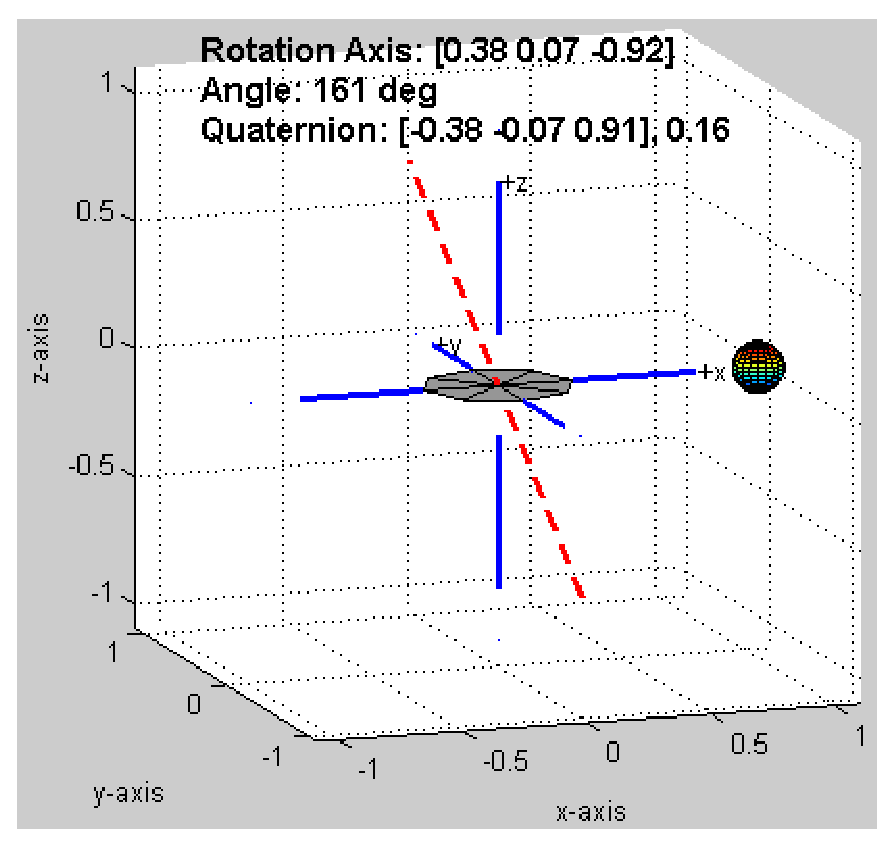
\psfig{file=figures/q_rotation_start.eps,height=3in}}
  \caption{TableSat Wireframe}
  \label{fig:TSatWireframe}
\end{figure}

The collection of the points in the TableSat wireframe can be rotated as the single point was from above.  Once new locations are determined, the TableSat wireframe can be redrawn visualizing the estimated current orientation of the TableSat (Figure \ref{fig:TSatWireframeEstimatedAttitude}).  Chapter \ref{chap:SoftwareDevelopmentforExperimentalIntegration} will cover the ``run-time'' visualizations in greater detail to show how as the estimator is running, updates to the estimated state, $\bs{\hat{x}}$, can be used to update the wireframe's orientation.

\begin{figure}[H]
  \centerline{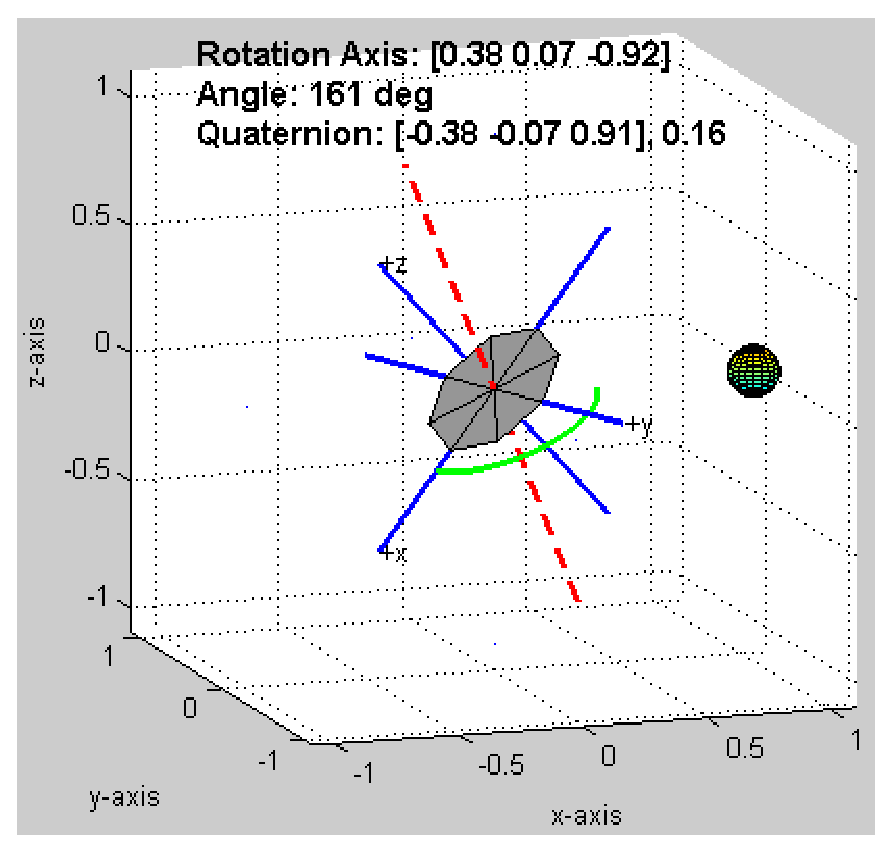
\psfig{file=figures/q_rotation_end.eps,height=3in}}
  \caption{TableSat Wireframe Estimated Attitude}
  \label{fig:TSatWireframeEstimatedAttitude}
\end{figure}


\subsubsection{Incremental Quaternion Rotations}
\label{subsubsec:IncrementalQuaternionRotations}

The quaternion's definition based on Euler's theorem of a rotation about a single axis makes tracking the orientation of a spin-stabilized satellite an easier process.  NASA's MMS mission has a target spin rate of 3 rpm (~0.314 rad/sec).  A rotational quaternion representing the per second rotation about the z-axis is

\begin{equation}
  \begin{aligned}
    \bs{q}_{rps} = & ( 0\bs{i} + 0\bs{j} + 1\bs{k} ) \sin \left( \frac{-0.314}{2} \right) + \cos \left( \frac{-0.314}{2} \right) \\
    = & 0\bs{i} +0\bs{j} -0.156434\bs{k} + 0.987688
  \end{aligned}
\end{equation}

In an open loop system, the best estimate of the systems state would be to apply the quaternion rotation each second to the previous steps state starting with an initially known orientation.  For example if we have the TableSat at a $+1/4$ turn about the z-axis, each second we can calculate the best guess at the current attitude using just a quaternion multiplication.

\begin{equation}
  \begin{aligned}
    \bs{q}(t_{k+1}) = & \bs{q}_{rps} \otimes \bs{q}(t_{k}) \\
    \text{where } \bs{q}(t_0) = & 0 \bs{i} +0 \bs{j} -0.707107 \bs{k} +0.707107
  \end{aligned}
  \label{eqn:3rpmQuaternionEquation}
\end{equation}

\subsubsection{Quaternion Decomposition}
\label{subsubsec:QuaternionDecomposition}

The attitude of TSat is represented by a single quaternion.  The change in attitude between two states can be modeled by the a rotation about a single axis.  Figure \ref{fig:PreDecomposedQuaternion} show the attitude of a system described by the quaternion $\bs{q} = [\alpha, \beta, \phi], 0.16953$ which is a rotation of 2.8 radians about the axis $[\alpha, \beta, \phi]^T$.  For control purposes, decomposing the single quaternion into one representing a rotation about the z-axis and a second rotation about an axis in the x-y plane as shown in Figure \ref{fig:PostDecomposedQuaternion}.

\begin{figure}[H]
  \begin{subfigure}[h!]{0.5\textwidth}
    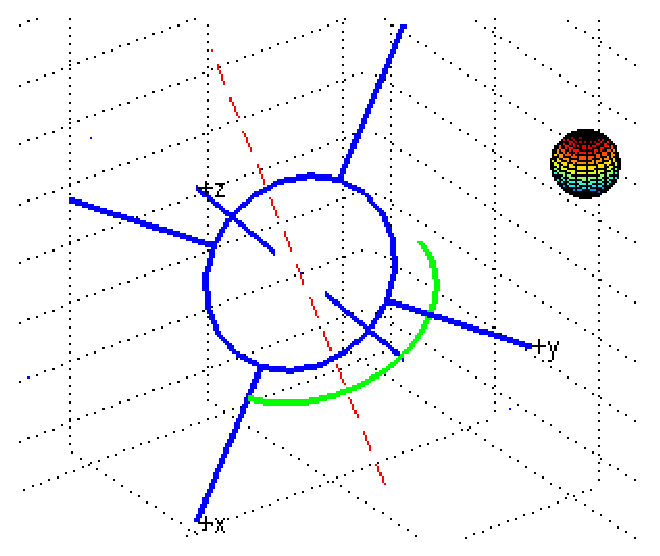
\includegraphics[width=\textwidth]{figures/quaternion_decompose_pre.eps}
    \caption{Quaternion State}
    \label{fig:PreDecomposedQuaternion}
  \end{subfigure}
  ~
  \begin{subfigure}[h!]{0.5\textwidth}
    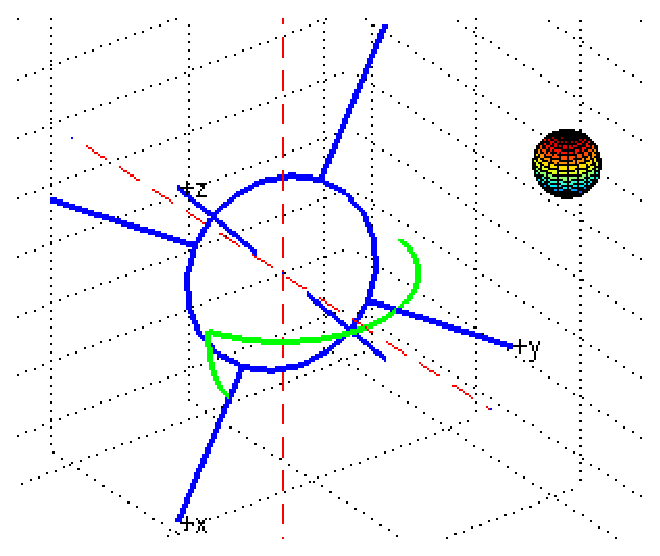
\includegraphics[width=\textwidth]{figures/quaternion_decompose_post.eps}
    \caption{Decomposed State}
    \label{fig:PostDecomposedQuaternion}
  \end{subfigure}
  \caption{Decomposing a Quaternion into Rotation and Nutation}
  \label{fig:QuaternionDecomposition}
\end{figure}

The quaternion that describes TSat's attitude $\bs{q}$ can be written as a sequence of two rotations.  A quaternion rotation about the z-axis $\bs{q_r}$ followed by the quaternion rotation about an axis in the x-y plane that creates a nutation $\bs{q_n}$.  Resultant rotations are performed through a left quaternion multiplication.
\begin{equation}
  \bs{q} = \bs{q_n} \otimes \bs{q_r} = \begin{bmatrix} \bs{v}_n \\ q_{0n} \end{bmatrix} \otimes \begin{bmatrix} \bs{v}_r \\ q_{0r} \end{bmatrix}
\end{equation}
\begin{equation}
  \begin{bmatrix}\bs{v} \\ q_{0} \end{bmatrix} =
  \begin{bmatrix} \bs{v}_n q_{0r} + \bs{v}_r q_{0n} + \bs{v}_n \times \bs{v}_r \\  q_{0n} q_{0r} - \bs{v}_n \cdot \bs{v}_r \end{bmatrix}
  \label{eqn:rot_nut_product}
\end{equation}
Expanding the vector components out creates the equation.
\begin{equation}
  \begin{bmatrix}
    q_{1} \\
    q_{2} \\
    q_{3} \\
    q_{0}
  \end{bmatrix}
  =
  \begin{bmatrix}
    \begin{bmatrix}
      q_{1n} \\
      q_{2n} \\
      q_{3n} \\
    \end{bmatrix} q_{0r} + \begin{bmatrix}
      q_{1r} \\
      q_{2r} \\
      q_{3r} \\
    \end{bmatrix} q_{0n} + \begin{bmatrix}
      q_{1n} \\
      q_{2n} \\
      q_{3n} \\
    \end{bmatrix} \times \begin{bmatrix}
      q_{1r} \\
      q_{2r} \\
      q_{3r} \\
    \end{bmatrix}
    \\
    q_{0n} q_{0r} - \begin{bmatrix}
      q_{1n} \\
      q_{2n} \\
      q_{3n} \\
    \end{bmatrix} \cdot \begin{bmatrix}
      q_{1r} \\
      q_{2r} \\
      q_{3r} \\
    \end{bmatrix} \\
  \end{bmatrix}
\end{equation}
and through simplification becomes
\begin{equation}
  \begin{bmatrix}
    q_{1} \\
    q_{2} \\
    q_{3} \\
    q_{0}
  \end{bmatrix}
  =
  \begin{bmatrix}
    q_{1n} q_{0r} + q_{1r} q_{0n} + q_{2n} q_{3r} - q_{3n} q_{2r} \\
    q_{2n} q_{0r} + q_{2r} q_{0n} + q_{3n} q_{1r} - q_{1n} q_{3r} \\
    q_{3n} q_{0r} + q_{3r} q_{0n} + q_{1n} q_{2r} - q_{2n} q_{1r} \\
  q_{0n} q_{0r} - (q_{1n} q_{1r} + q_{2n} q_{2r} + q_{3n} q_{3r} ) \\
  \end{bmatrix}
  \label{eqn:rot_nut_product_simplified}
\end{equation}
Now that we have an expanded representation of the resultant quaternion, we can use the restriction from the desired spin-stabilized state for TableSat/MMS.  The rotational quaternion is allowed to move freely about the $z$-axis but should not have any displacement about the $x$ and $y$ axes.  From Equation \ref{eqn:RotationalQuaternionDefinition}, $q_{1r} = q_{2r} = 0$.
\begin{equation}
  \bs{q_{r}}
  = q_{1r} \bs{i} + q_{2r} \bs{j} + q_{3r} \bs{k} + q_{0r}
  = 0 \bs{i} + 0 \bs{j} + q_{3r} \bs{k} + q_{0r}
  \label{eqn:rotation_quaternion_defined}
\end{equation}
The nutation quaternion has the opposite restrictions where rotation is allowed about the $x$ and $y$ axes but not about the $z$ axis.  From Equation \ref{eqn:RotationalQuaternionDefinition}, $q_{3n} = 0$.
\begin{equation}
  \bs{q_{n}}
  = q_{1n} \bs{i} + q_{2n} \bs{j} + q_{3n} \bs{k} + q_{0n}
  = q_{1n} \bs{i} + q_{2n} \bs{j} + 0 \bs{k} + q_{0n}
  \label{eqn:nutation_quaternion_defined}
\end{equation}
Substituting equations \eqref{eqn:rotation_quaternion_defined} and \eqref{eqn:nutation_quaternion_defined} into \eqref{eqn:rot_nut_product_simplified} yields.
\begin{equation}
  \begin{bmatrix}
    q_{1} \\
    q_{2} \\
    q_{3} \\
    q_{0}
  \end{bmatrix}
  =
  \begin{bmatrix}
    q_{1n} q_{0r} + 0             + q_{2n} q_{3r} - 0 \\
    q_{2n} q_{0r} + 0             + 0             - q_{1n} q_{3r} \\
    0             + q_{3r} q_{0n} + 0             - 0 \\
  q_{0n} q_{0r} - (q_{1n} 0 + q_{2n} 0 + 0 q_{3r} ) \\
  \end{bmatrix}
\end{equation}
\begin{subequations}
  \begin{align}
    q_{1} &= q_{1n} q_{0r} + q_{2n} q_{3r} \label{eqn:rot_nut_1_1} \\
    q_{2} &= q_{2n} q_{0r} - q_{1n} q_{3r} \label{eqn:rot_nut_1_2} \\
    q_{3} &= q_{3r} q_{0n} \label{eqn:rot_nut_1_3} \\
    q_{0} &= q_{0n} q_{0r} \label{eqn:rot_nut_1_0}
  \end{align}
\end{subequations}
Solving \ref{eqn:rot_nut_1_3} and \ref{eqn:rot_nut_1_0} for $q_{3r}$ and $q_{0r}$ and substituting into \ref{eqn:rot_nut_1_1} and \ref{eqn:rot_nut_1_2}
\begin{subequations}
  \begin{align}
    q_{0n} q_{1} &= q_{1n} q_{0} + q_{2n} q_{3} \label{eqn:rot_nut_2_1} \\
    q_{0n} q_{2} &= q_{2n} q_{0} - q_{1n} q_{3} \label{eqn:rot_nut_2_2}
  \end{align}
\end{subequations}
combining \ref{eqn:rot_nut_2_1} and \ref{eqn:rot_nut_2_2}
\begin{equation}
  0 = (q_{0}q_{2} + q_{1}q_{3}) q_{1n} + (q_{2}q_{3} - q_{0}q_{1}) q_{2n}
\end{equation}
\begin{subequations}
  \begin{align}
    q_{1n} &= Q \cdot q_{2n} \\
    \text{where } Q &= \frac{q_{0}q_{1} - q_{2}q_{3}}{q_{0}q_{2} + q_{1}q_{3}}
  \end{align}
  \label{eqn:nutation_parameter_ratio}
\end{subequations}
The additional restriction than rotational quaternions have a unit norm can be leveraged in finding solutions
\begin{equation}
  \left\| \bs{q} \right\| = \sqrt{\bs{v} \cdot \bs{v} + q_0^2} = \sqrt{q_1^2+q_2^2+q_3^2+q_0^2}
  \label{eqn:quaternion_norm}
\end{equation}
Taking the norm of the rotational quaternion in Equation \ref{eqn:rotation_quaternion_defined} and substituting $q_{3r}$ and $q_{0r}$ from Equations \ref{eqn:rot_nut_1_3} and \ref{eqn:rot_nut_1_0} becomes
\begin{equation}
  (0)^2 + (0)^2 + \left( \frac{q_3}{q_{0n}} \right)^2 + \left( \frac{q_0}{q_{0n}} \right)^2 = 1
\end{equation}
solving for $q_{n0}$
\begin{equation}
  q_{n0} = \pm \sqrt{q_3^2 + q_0^2}
  \label{eqn:nutation_scalar}
\end{equation}
substituting \ref{eqn:nutation_parameter_ratio} and \ref{eqn:nutation_scalar} into \ref{eqn:nutation_quaternion_defined}
\begin{equation}
  \bs{q_{n}}
  = Q \cdot q_{2n} \bs{i} + q_{2n} \bs{j} + 0 \bs{k} \pm \sqrt{q_3^2 + q_0^2}
\end{equation}
and as this is a rotational quaternion, its norm should always equal one
\begin{equation}
  (Q \cdot q_{2n})^2 + (q_{2n})^2 + (q_3^2 + q_0^2) = 1
\end{equation}
which can be solved for the nutation quaternion's $q_{2n}$ term
\begin{equation}
  q_{2n} = \pm \sqrt{ \frac{1  - q_3^2 - q_0^2}{Q^2 + 1} }
  \label{eqn:qn2_solution}
\end{equation}

We now have a mapping of the original state quaternion $\bs{q}$ to its decomposed rotation $\bs{q}_r$ and nutation $\bs{q}_n$ quaternions.  The ability to break the attitude parameters into these two quantities is particularly useful for spin-stabilized satellites as it decouples the rate and attitude controllers.  Normally the attitude controller would need to propagate the desired quaternion attitude with input from the body rates. In this approach, the controller can ignore continuously changing rotational component $\bs{q}_r$, and limit its focus on driving the nutation error $\bs{q}_n$ to zero (Figure \ref{fig:PostDecomposedQuaternion}).
\begin{subequations}
  \begin{align}
    q_{1n} &= Q \cdot q_{2n} \\
    q_{2n} &= \sqrt{ \frac{1  - q_3^2 - q_0^2}{Q^2 + 1} }\\
    q_{n0} &= \sqrt{q_3^2 + q_0^2} \\
    q_{3r} &= \frac{q_3}{q_{0n}} \\
    q_{0r} &= \frac{q_0}{q_{0n}} \\
    \text{where } Q &= \frac{q_{0}q_{1} - q_{2}q_{3}}{q_{0}q_{2} + q_{1}q_{3}}
  \end{align}
\end{subequations}


\section{Satellite Dynamics}
\label{sec:SatelliteDynamics}

The goal in creating an accurate satellite dynamics model is it's ability to predict the state of the system given the last know state, the elapsed time since the last known state, and any inputs or disturbances to the system.  The initial scope of predicting the satellite's state is restricting it to a state propagation problem where only last state and elapsed time are considered.  Estimation techniques in Section \ref{chap:Estimators} will cover how a propagated state can be adjusted using the measured state.

\subsection{System Clock}
\label{subsec:SystemClock}

As was mentioned at the end of section \ref{subsubsec:IncrementalQuaternionRotations}, perfectly timed updates are highly unlikely.  Small variations in the timestep size will cause predicted state errors.  A state update running every 1.0001 seconds instead of every second would accumulate over a six degree error after tracking TableSat's state for an hour.  Linearized model would also be affected because the expected timestep size is incorporated as part of the discretization processes.

The preset fixed timestep is also not very fault tolerant.  When controlling the state of a stable, slow moving system the state tracking rate could be slowed down to conserve system resources.  In this circumstance a missed or series of missed updates due to faults can cause the predicted state to be several $\Delta t$ behind where it should be.  A solution built for variable steps can improve the robustness against these errors.

The ability to slow down a simulation to closely watch the initial transient behavior followed speeding up the simulation to inspect long term stability hold benefits for both outreach and research purposes.  The TSatPy system was built with this idea in mind which addresses the previous two issues as the system by design needs to be able to smoothly transition between variations in step sizes in a single run.

\begin{equation}
  \begin{aligned}
    t_k =& \sum\limits_{i=0}^{k-1} r_i (\tau_{i+1} - \tau_i)\\
    \text{where } \tau =& \text{ real time} \\
    t_k =& \text{ simulation time at step }k
  \end{aligned}
  \label{eqn:SystemTime}
\end{equation}

The system clock defined in Equation \ref{eqn:SystemTime} starts at zero and accumulates time depending on the set rate.

\subsection{Body Rate and Quaternion Propagation}
\label{subsec:BodyRateQuaternionPropagation}

Predicting the body rates, $\omega_x, \omega_y, \omega_z$, for TableSat requires knowledge about the body dynamics, the last calculated body rate, time elapsed since last update, and any applied moments.  Equation \ref{eqn:DiscreteEulerMomentEquations} is used to propagate the body rate in a variable step.

In Chapter \ref{chap:ObserverBasedControls} these quaternion and body rate propagation techniques will be incorporated into the observer based control system.


\chapter{UNH TableSat 1A}
\label{chap:UNHTableSat1A}

The UNH TableSat 1A is a limited 3-DOF experimental test bed analog for the NASA MMS satellite (See Figure \ref{fig:TSatFullView}).  All electronics, booms, and actuators are attached to a circular PVC deck.  The aluminum hub at its center has a hollow center which allow it to rest on a center post giving the deck full rotation about its z-axis and limited rotations about its x and y-axes.  Five out of the six booms present on the MMS spacecraft are represented on TableSat 1A.  The four SDP booms extend radially from the deck at 90 degree intervals.  One of the MMS's ADP booms is modeled with a boom attached to the center post of the TableSat.



\begin{figure}[H]
\centerline{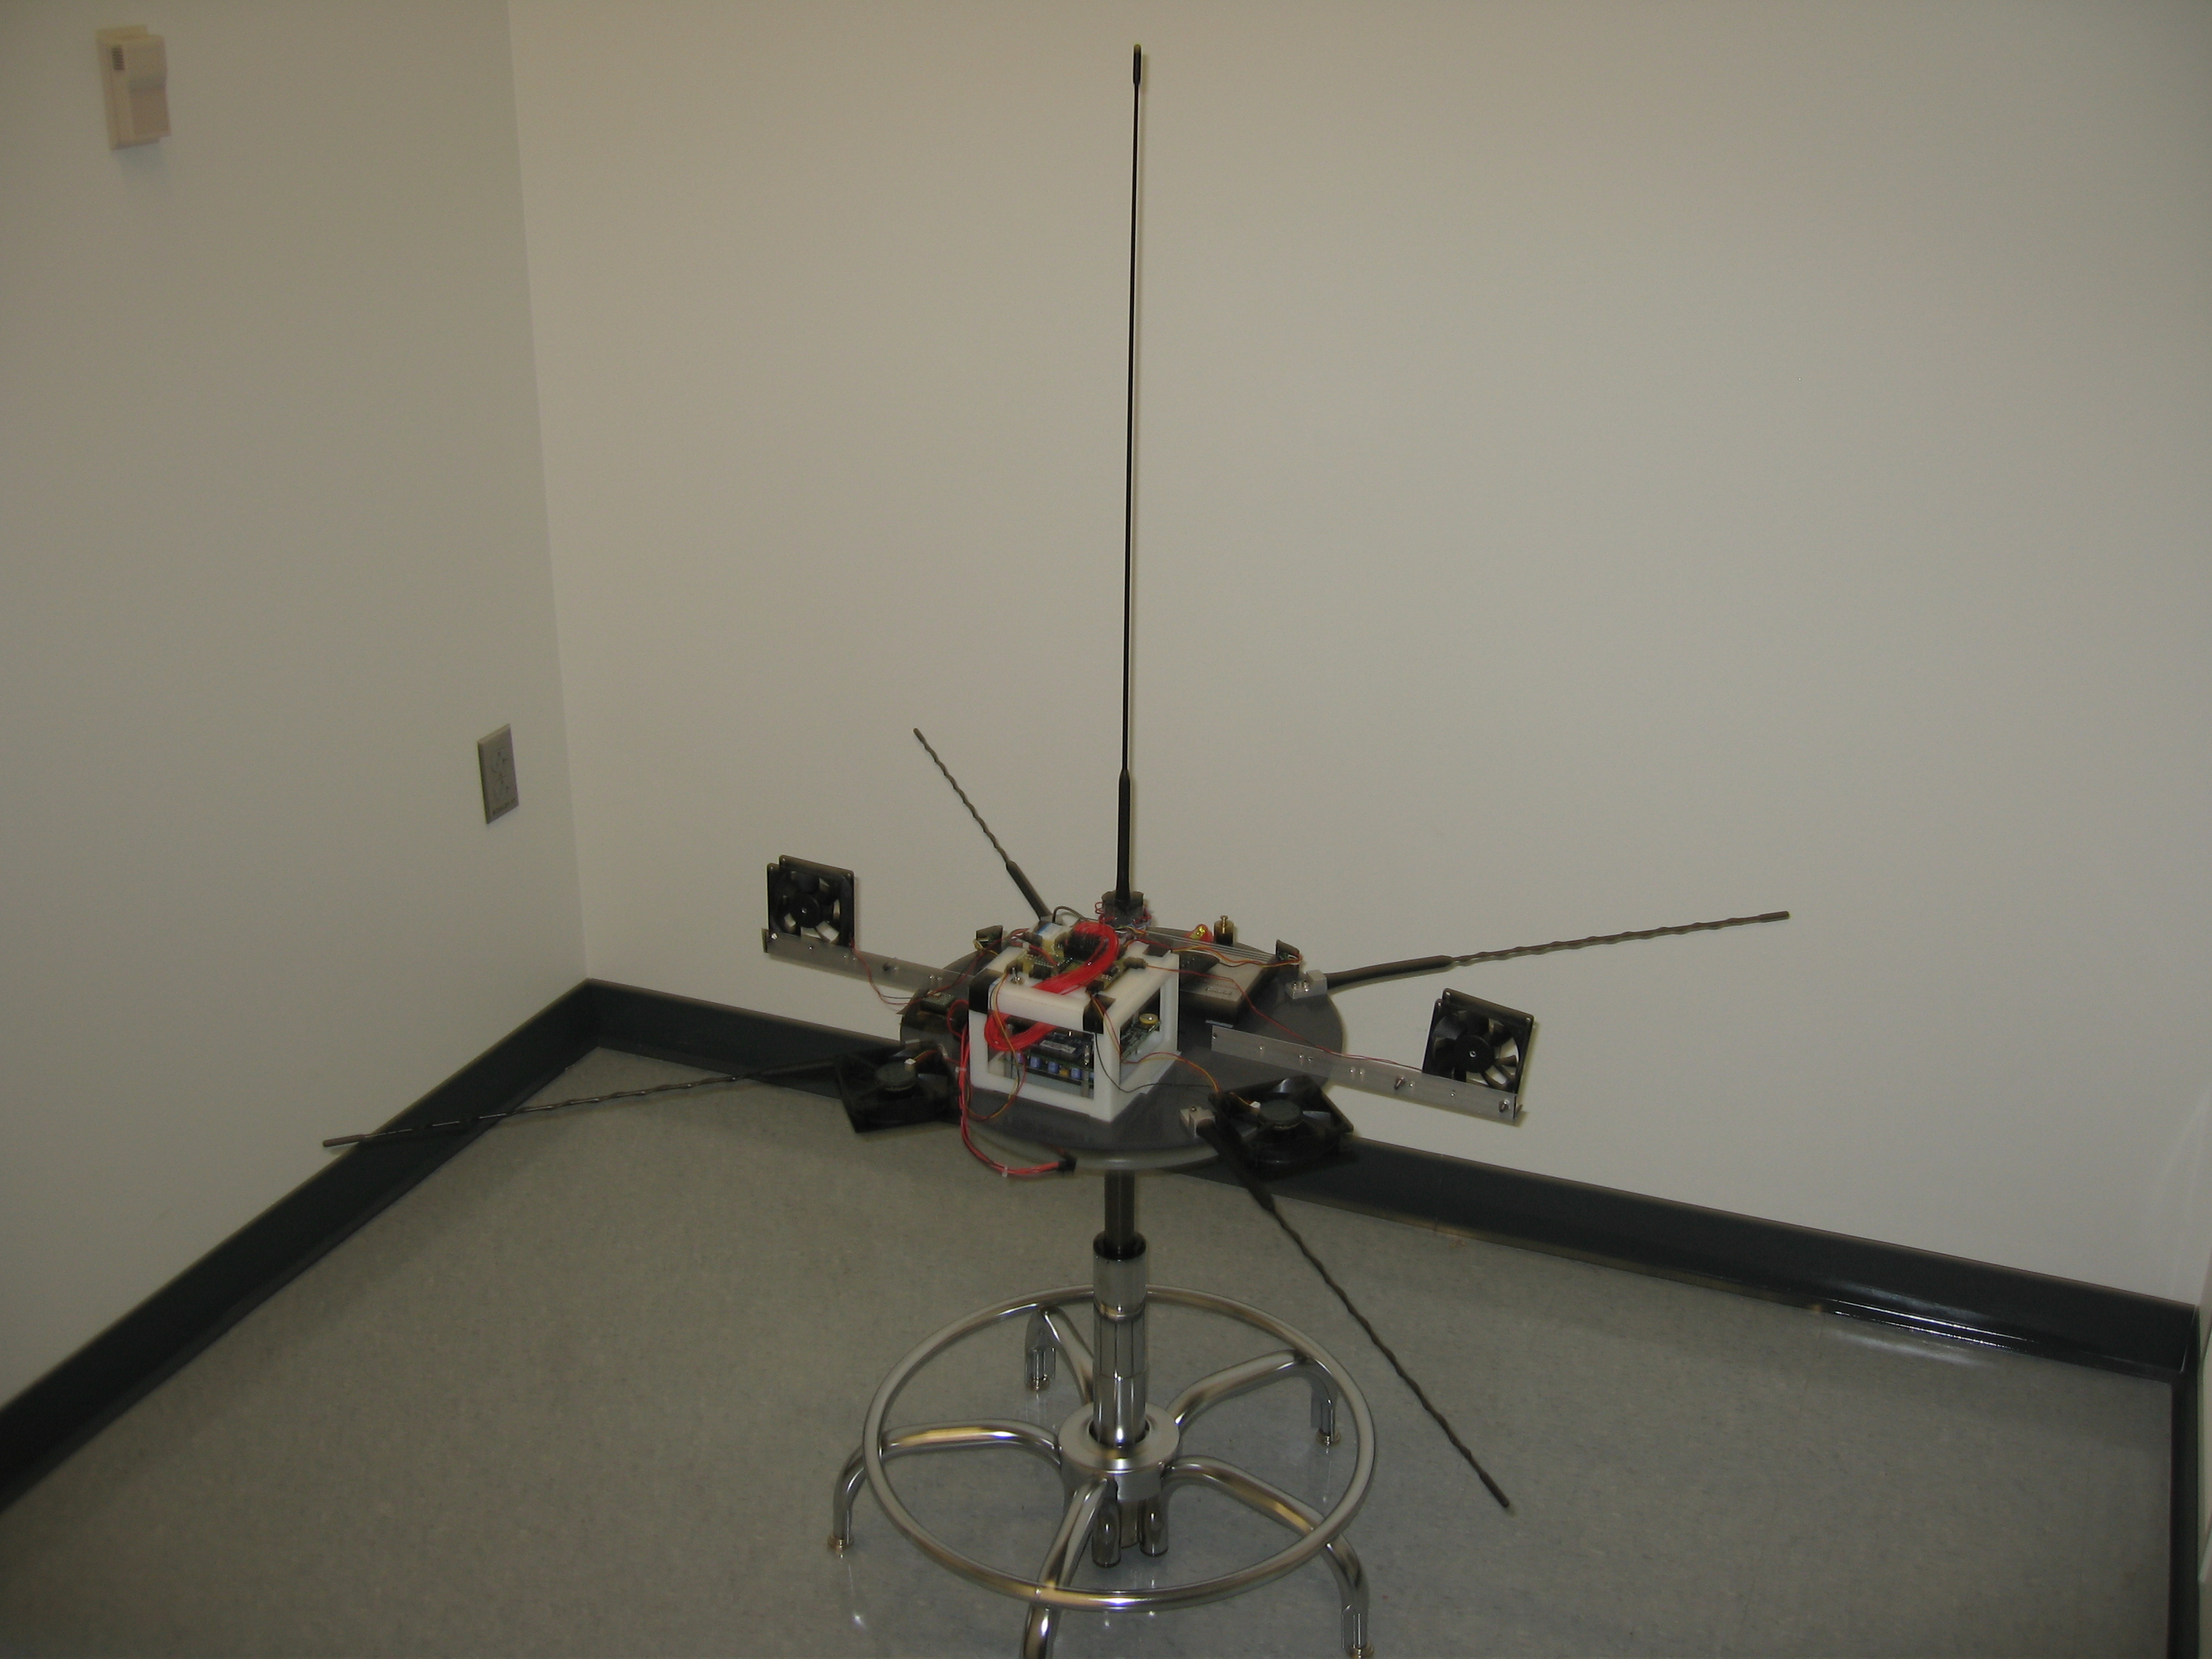
\psfig{file=figures/tsat_full_view.eps,height=3in}}
\caption{TableSat 1A Full View}
\label{fig:TSatFullView}
\end{figure}

\section{Booms}
\label{sec:Booms}

The ADP booms were modeled with a selection of flexible antenna.  Attaching weights to the tip and varying the stiffness of the selected antenna allowed for some tuning to the fundamental frequency of the booms.  Since the SDP booms extend perpendicularly to gravity, two choices were made for their modeling.  For free motion, the cylindrical antenna for the ADP boom were also used for the SDP booms.  The disadvantage to these booms especially when adding weights to reduce their natural frequency was that they would droop under the gravitational pull.  An alternative to the cylindrical antenna for the SPD booms were thin and flat strips of metal.  Attaching them to the TableSat's deck such that they were standing on edge removed the gravitational drooping since the booms, but still allowed for the boom to bend back and forth in the spin plane.  This also restricted the boom's freedom of movement, so a combination of results would be needed to get a better idea of how the MMS booms would react in orbit.

\begin{figure}[H]
\centerline{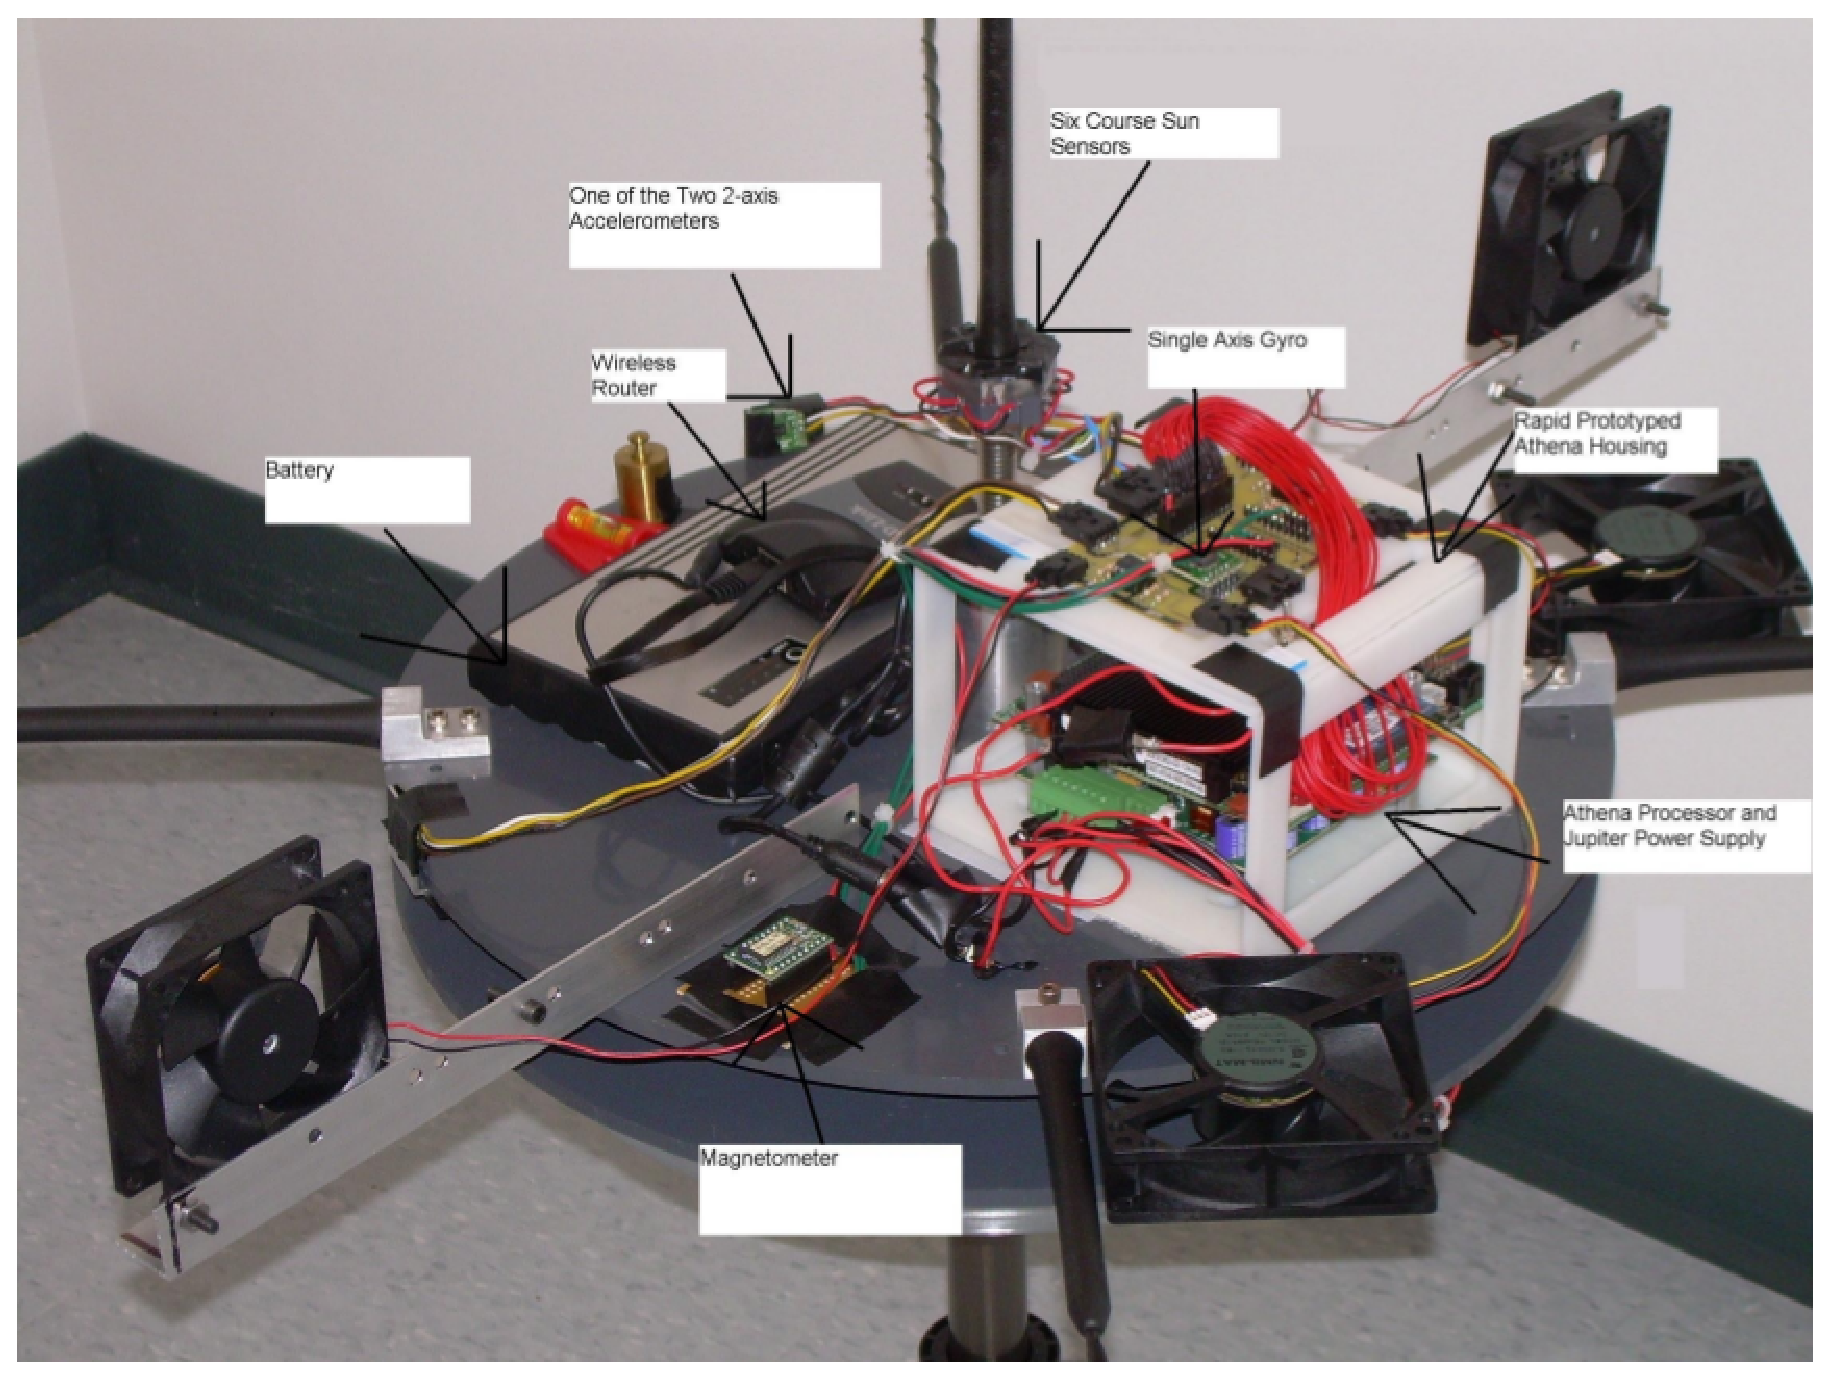
\psfig{file=figures/tsat_components.eps,height=4in}}
\caption{TableSat Components}
\label{fig:TSatComponents}
\end{figure}

\section{Flight Controller}
\label{sec:FlightController}

The onboard flight controller was an Athena PC from Diamond Systems powered by a Jupiter power supply and lithium-ion rechargeable battery.  The Athena processor and Jupiter power supply were mounted in a rapid prototyping housing with open sides for ventilation.  A custom printed circuit board designed by Jeff Kite \TODO{need footnote reference here?} was mounted on top of the rapid prototyping housing.  User Datagram Protocol (UDP) communication (Section \ref{subsec:MessageDefinitions}) to the base station is transmitted through a wireless access point.

\TODO{forgot cs student's name} created a C program based off of Vess' ``open-loop'' flight controller \cite{vessthesis} .  This program is responsible for listening to a UDP socket on the TableSat and performing a limited set of actions based on the message packets received from the base station.  The most common messages triggered actions like altering the voltages applied to the actuators, and scanning the sensor ports and sending the voltages back to the base station through UDP.

\section{Actuators}
\label{sec:Actuators}

In addition to the booms extending from the TableSat's deck, four single direction analog input computer fans were mounted to provide a source of thrust (Figure \ref{fig:TSatComponents}).  Two fans were mounted standing upright to provide radial torque.  One pointing clockwise and the other counter clockwise had their centers level with the pivot point inside the central hub and provided control of the rotation rate.  Two other fans were mounted facing down to provide limited opportunities for nutation control.

\section{Sensors}
\label{sec:Sensors}

Four classes of analog sensors were implemented in TableSat 1A's design. Gyroscope (Section \ref{subsec:Gyroscope}) and accelerometer (Section \ref{subsec:Accelerometer}) for velocity measurements.  Course sun sensor (Section \ref{subsec:CourseSunSensor}), and magnetometer (Section \ref{subsec:TripleAxisMagnetometer}) for position measurements.  These sensors and the four actuators filled all available analog ports on the onboard Athena flight computer.  As is described below, the gyroscopes and accelerometers were not used for the observer-based controllers in this thesis leaving just positional measurements from the course sun sensors and triple axis magnetometer.

\begin{figure}[H]
\centerline{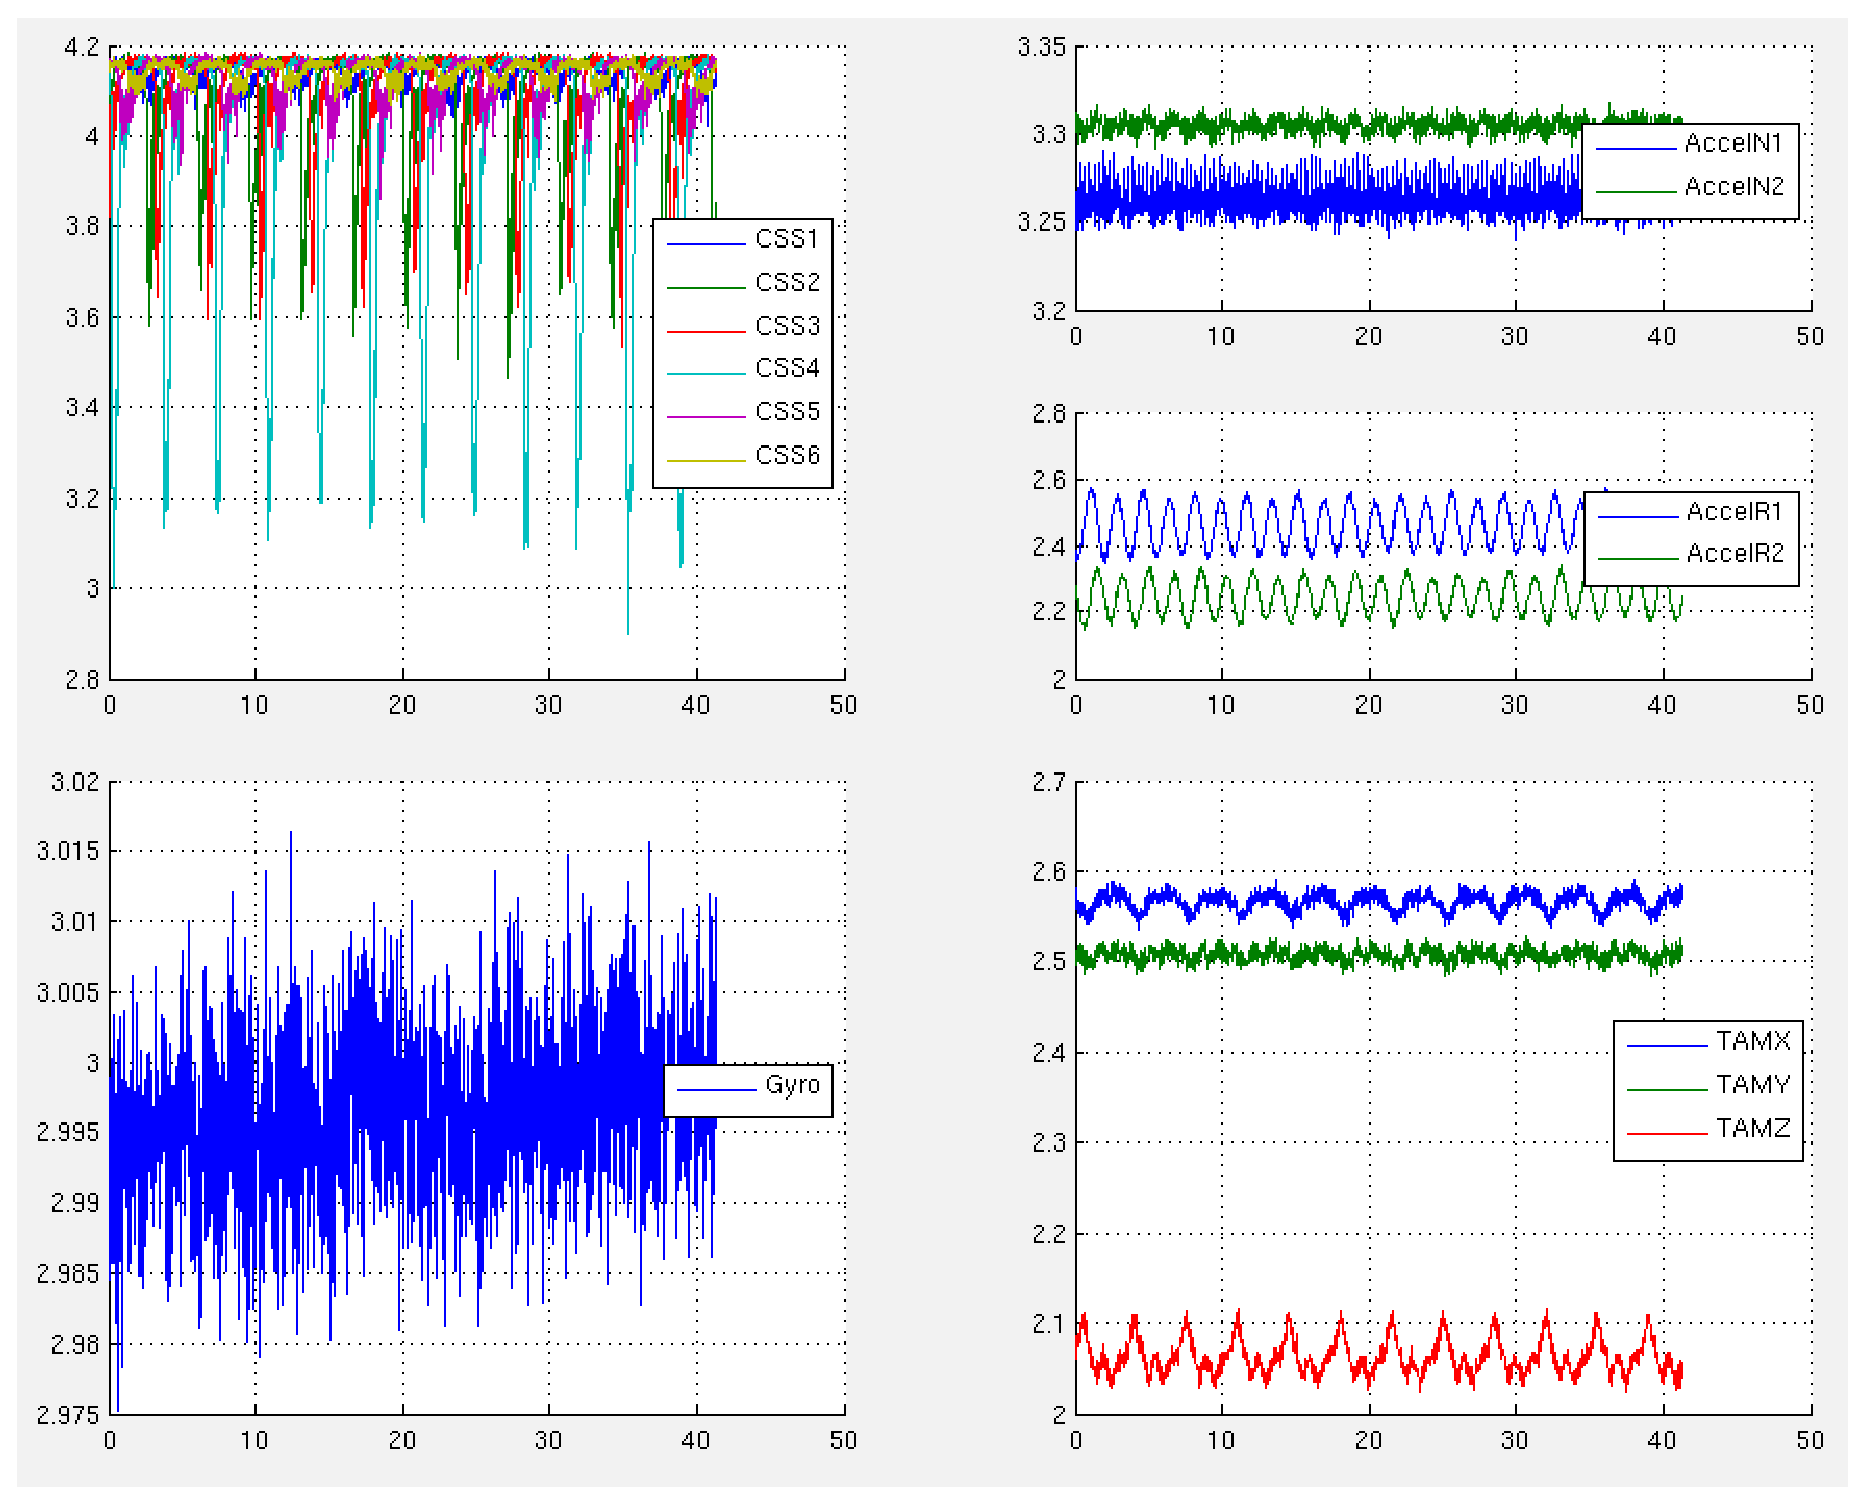
\psfig{file=figures/sensor_voltage_charts.eps,height=4in}}
\caption{Sensor Voltage Readings}
\label{fig:SensorVoltageReadings}
\end{figure}

\subsection{Gyroscope}
\label{subsec:Gyroscope}

Gyroscopes remain one of the most accurate sensors for detecting changes to a structure's angular body rates.  The issue with their use is that to increasing the accuracy of a gyroscope means using a heavier sensor.  Since any additional weight is a serious launch concern for a satellite, this research for NASA's MMS mission uses the gyro scope solely as a verification method.  The gyroscope selected for TableSat 1A is a single axis gyroscope that is mounted on the printed circuit board at the top of the flight controller housing.  The gyroscope is oriented to detect changes in body rates about the TableSat's z-axis although is mounted slightly above the center hub's pivot point so will pick up small signals from any limited nutation encountered.

\subsection{Accelerometer}
\label{subsec:Accelerometer}

Two 2-axis accelerometers are mounted at the circumference or TableSat's deck.  The accelerometers are oriented such that one signal detects vertical acceleration with a 2g resolution and the other a radial signal with a 0.5g resolution.  The rotational accelerometers ended up picking up a small signal which is either due to oscillations in angular velocity or a nutation subjecting the radial accelerometer to gravitational effects.  The vertical components of the accelerometers had such low signal to noise ratios that heavy filtering would be required to even attempt to detect the out of plane rotations.  Any significant nutations allowed by the limited 3-DOF design would damp out quickly enough to be eliminated before the filtering could identify the signal.  Given these severe limitations in the sensor's measurements, for the purpose of this thesis the accelerometer measurements are ignored.

\subsection{Course Sun Sensor}
\label{subsec:CourseSunSensor}

The course sun sensor (CSS) for UNH TableSat 1A was constructed from a hexagonal piece of PVC pipe with a photodiode mounted in each face (Figure \ref{fig:CSS}).  Photodiodes are light detectors that convert captured light to electricity.  Given the inability to use the gyroscope and the accelerometer's high level of noise, the course sun sensor proved to be the most reliable sensor, but was limited to measuring a single value from the state matrix corresponding to rotations about the z-axis.  Each photo diode detected light level in its field of view and would generate a voltage generally proportional to that value.  The photodiodes are mounted above the center hub and faced out around the spin plane.  By placing a single light source in a dark room, the course sun sensor's voltages could be used to calculate the angular displacement about the body's z-axis.


\begin{figure}[H]
\centerline{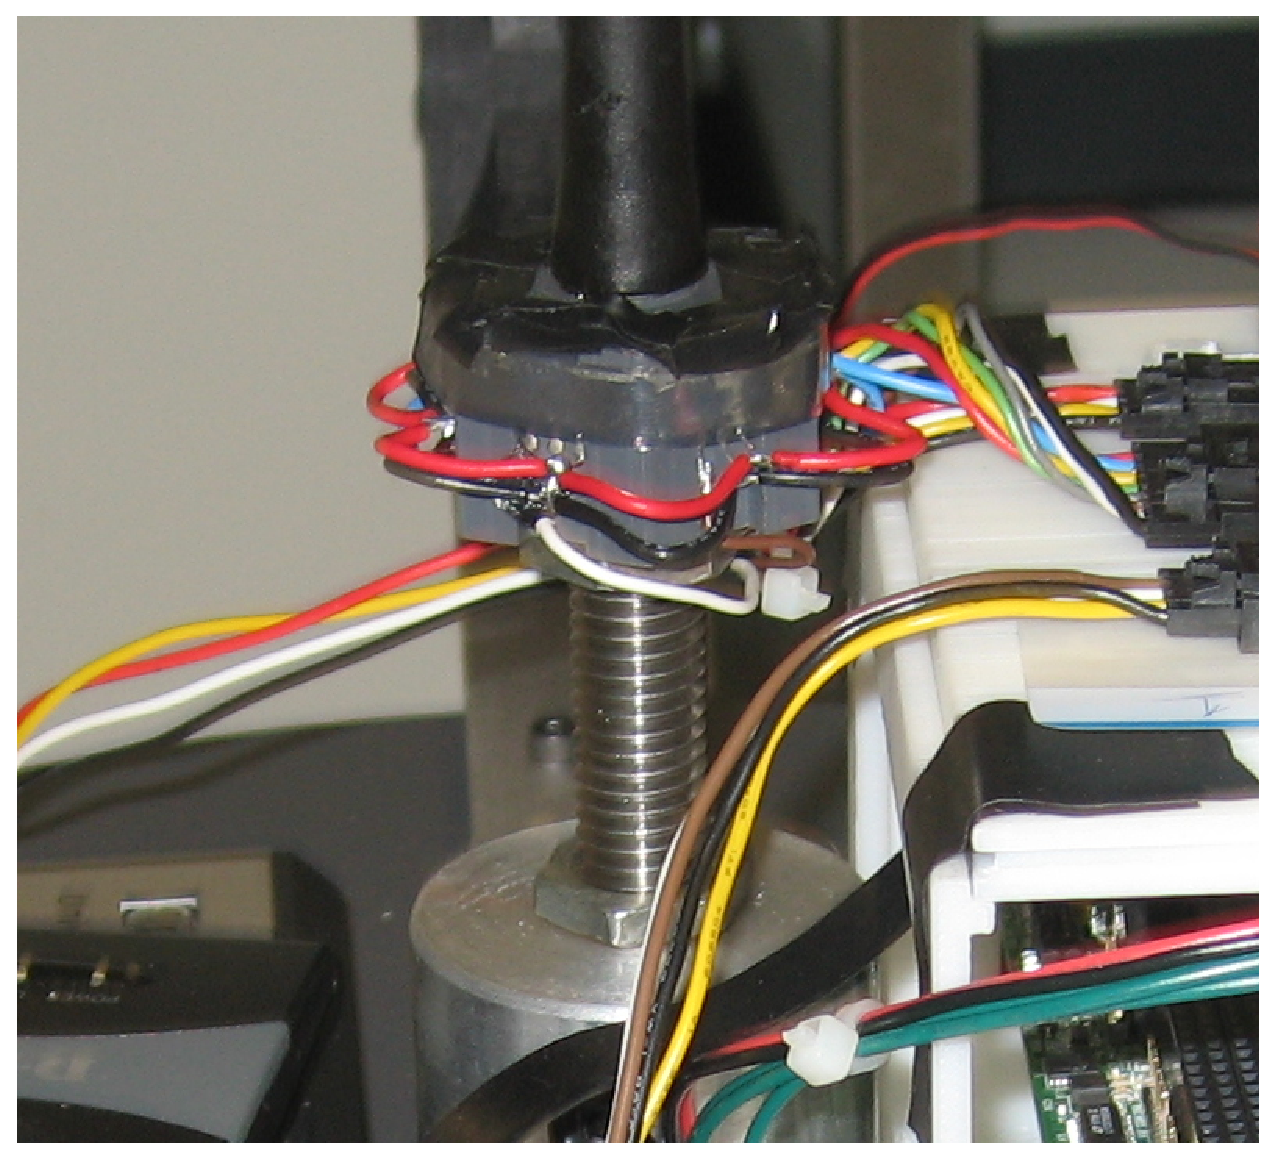
\psfig{file=figures/css.eps,height=2in}}
\caption{Course Sun Sensor Configuration}
\label{fig:CSS}
\end{figure}

Calculating the angular displacement about the body's z-axis is done using a method similar to a resultant force calculation.  Assuming all of the photodiodes volts per lumen rates are consistent, the voltages can be described as an equivalent force it the direction of the photodiode face.  Each force is decomposed into x and y components and then summed into a resultant force vector who's angle is used to represent the angular displacement of the TableSat.  Even though this method is fairly simplistic and that individual sensor voltage readings contained a moderate level of noise, this method proved to generate a very reliable and clean signal before even using filtering and estimation techniques.

\begin{subequations}
  \begin{align}
    V_{css\_x} & = \sum\limits_{i=1}^6 (V_{css\_x} - V_{css\_base}) \cos \left( \frac{2\pi}{6} (i-1)\right) \\
    V_{css\_y} & = \sum\limits_{i=1}^6 (V_{css\_x} - V_{css\_base}) \sin \left( \frac{2\pi}{6} (i-1)\right) \\
    \psi & = \tan^{-1} \frac{V_{css\_y}}{V_{css\_x}}
  \end{align}
  \label{eqn:CSSResultantForce}
\end{subequations}

\begin{figure}[H]
\centerline{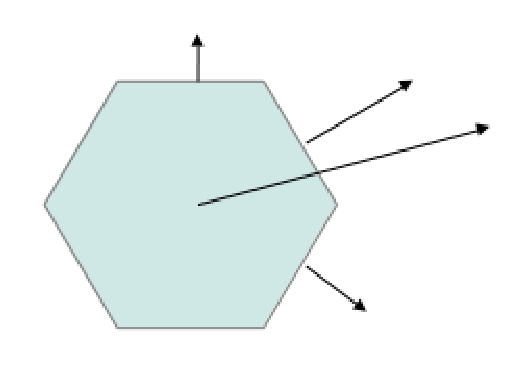
\psfig{file=figures/css_vectors.eps,height=1in}}
\caption{Photodiode Resultant Force Calculation for Yaw}
\label{fig:CSSVectors}
\end{figure}


\subsection{Triple Axis Magnetometer}
\label{subsec:TripleAxisMagnetometer}

Along with the course sun sensor, the triple-axis magnetometer (TAM) is used to measure position.  The primary advantage to the TAM over the course sun sensor it that it measures the full position state rather than just position about the z-axis.  As seen in Figure \ref{fig:SensorVoltageReadings}, three voltages are reported to designate the TableSat's attitude.  Each voltage corresponds to the strength of the magnetic field in each orthogonal direction.  To determine a method of converting raw TAM voltages to a TableSat, the clockwise actuator was set to provide a constant thrust.  With the fraction of the pivot point, the system slowly stabilized to a relatively constant spin rate.  Once stabilized, TAM voltage readings were recorded at a rate of 50 Hz and written to a log.  The mean values were subtracted from each of the three axes and plotted (Figure \ref{fig:TAMRaw}).

\begin{figure}[H]
\centerline{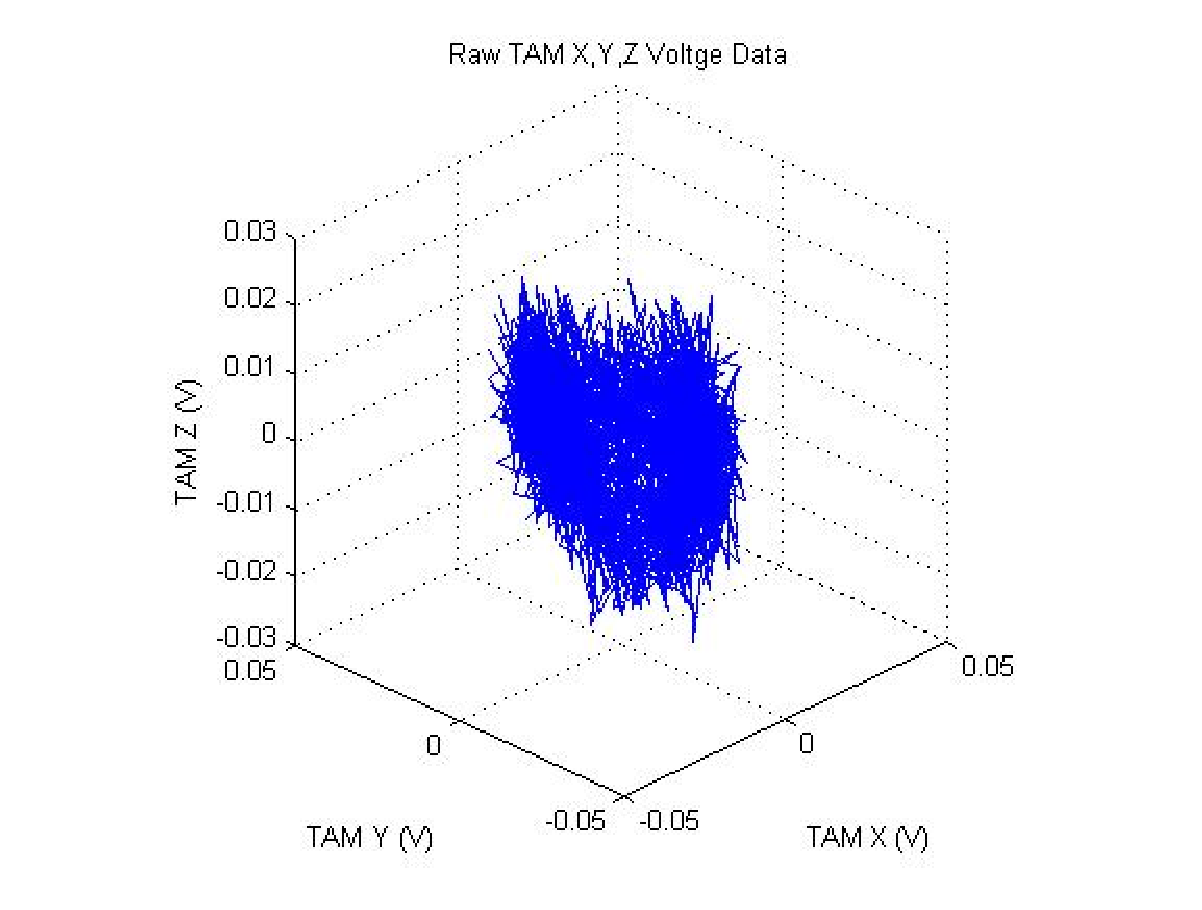
\psfig{file=figures/tam_raw.eps,height=4in}}
\caption{Raw TAM Voltages}
\label{fig:TAMRaw}
\end{figure}

Besides the slightly less dense center, the raw TAM measurements amount to a blob of points with no clear pattern.  If the signal is strong enough, a consistent path should be present.  Given the high sampling rate, aggressive filtering should be able to pull a signal out of the blob of data points.  A basic 40 point moving average was used as a first pass analysis to verify there is a signal in the data (Eq \ref{eqn:TAMMovingAvg}).  The moving average smoothed data is show in Figure \ref{fig:TAMMovingAverage}.  The good news being that a distinct an repeatable signal occurs as TableSat completes successive rotations.  The bad news is the irregular path that the magnetometer readings follow.

\begin{equation}
  x_i = \frac{1}{40} \sum^{39}_{j=0} x_{i-j}
  \label{eqn:TAMMovingAvg}
\end{equation}

\begin{figure}
  \begin{subfigure}[h!]{0.5\textwidth}
    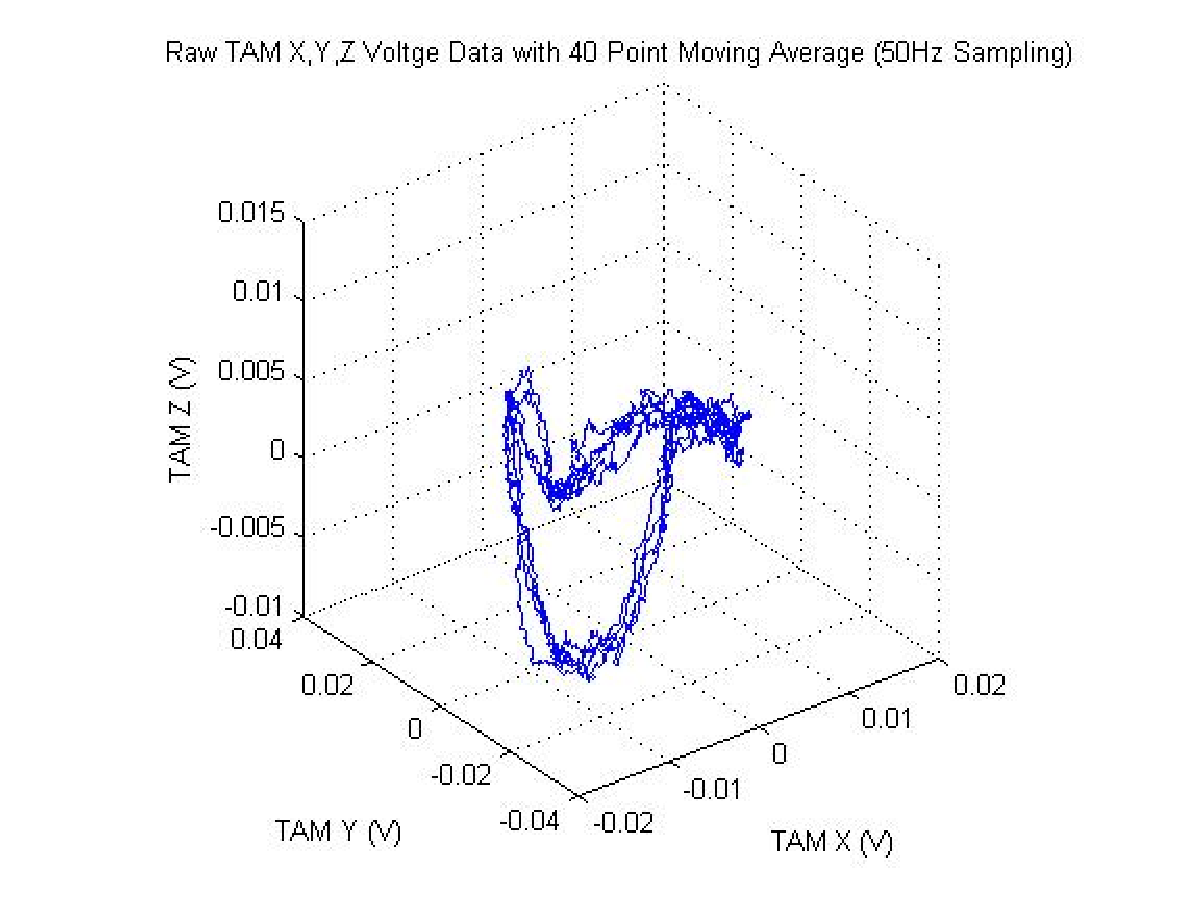
\includegraphics[width=\textwidth]{figures/tam_moving_average.eps}
    \caption{Raw TAM Voltages - Moving Average}
    \label{fig:TAMMovingAverage}
  \end{subfigure}
  ~
  \begin{subfigure}[h!]{0.5\textwidth}
    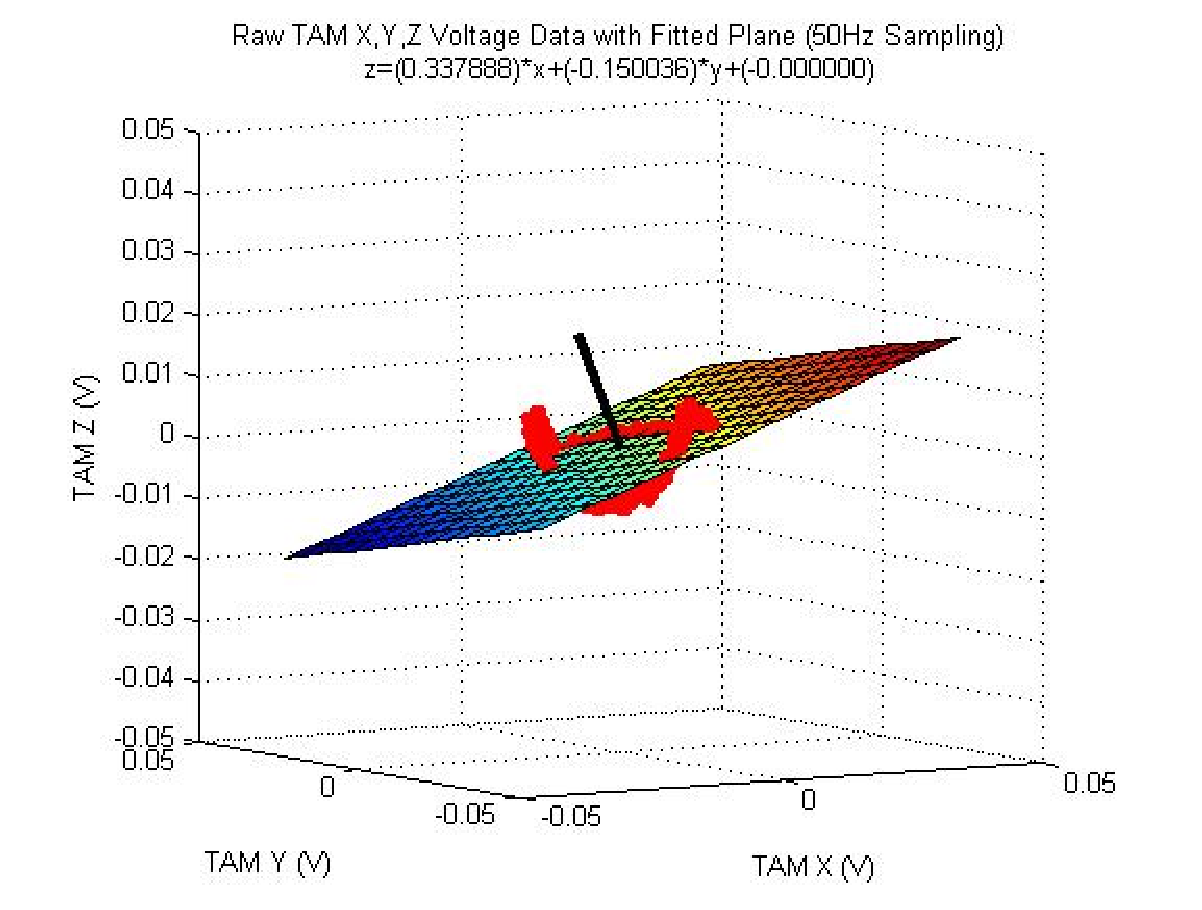
\includegraphics[width=\textwidth]{figures/tam_fitted_plane.eps}
    \caption{TAM Voltages with Fitted Plane}
    \label{fig:TAMFittedPlane}
  \end{subfigure}
  \caption{Determining Attitude from TAM}
  \label{fig:TAMSignal}
\end{figure}

Figure \ref{fig:TAMFittedPlane} shows the result of fitting a plane to the moving average smoothed TAM voltages.  The error in the fit between the smoothed TAM data points and the planar fit were too large to have much confidence in using this measure for nutation detection.

Following this analysis, the magnetic field surrounding the experimental setup was tested.  Moving a compass through the test space showed large swings in magnetic field lines despite the setup being placed on a wooden table in the middle of the lab.  Subsequent sweeps of the lab located a space with a relatively uniform magnetic field.  A uniform thrust was applied to the clockwise actuator and voltages logged as before.  Performing the moving average smoothing provided verification of the expected behavior of the magnetometer (Fig \ref{fig:TAMUniformField})

\begin{figure}[H]
  \centerline{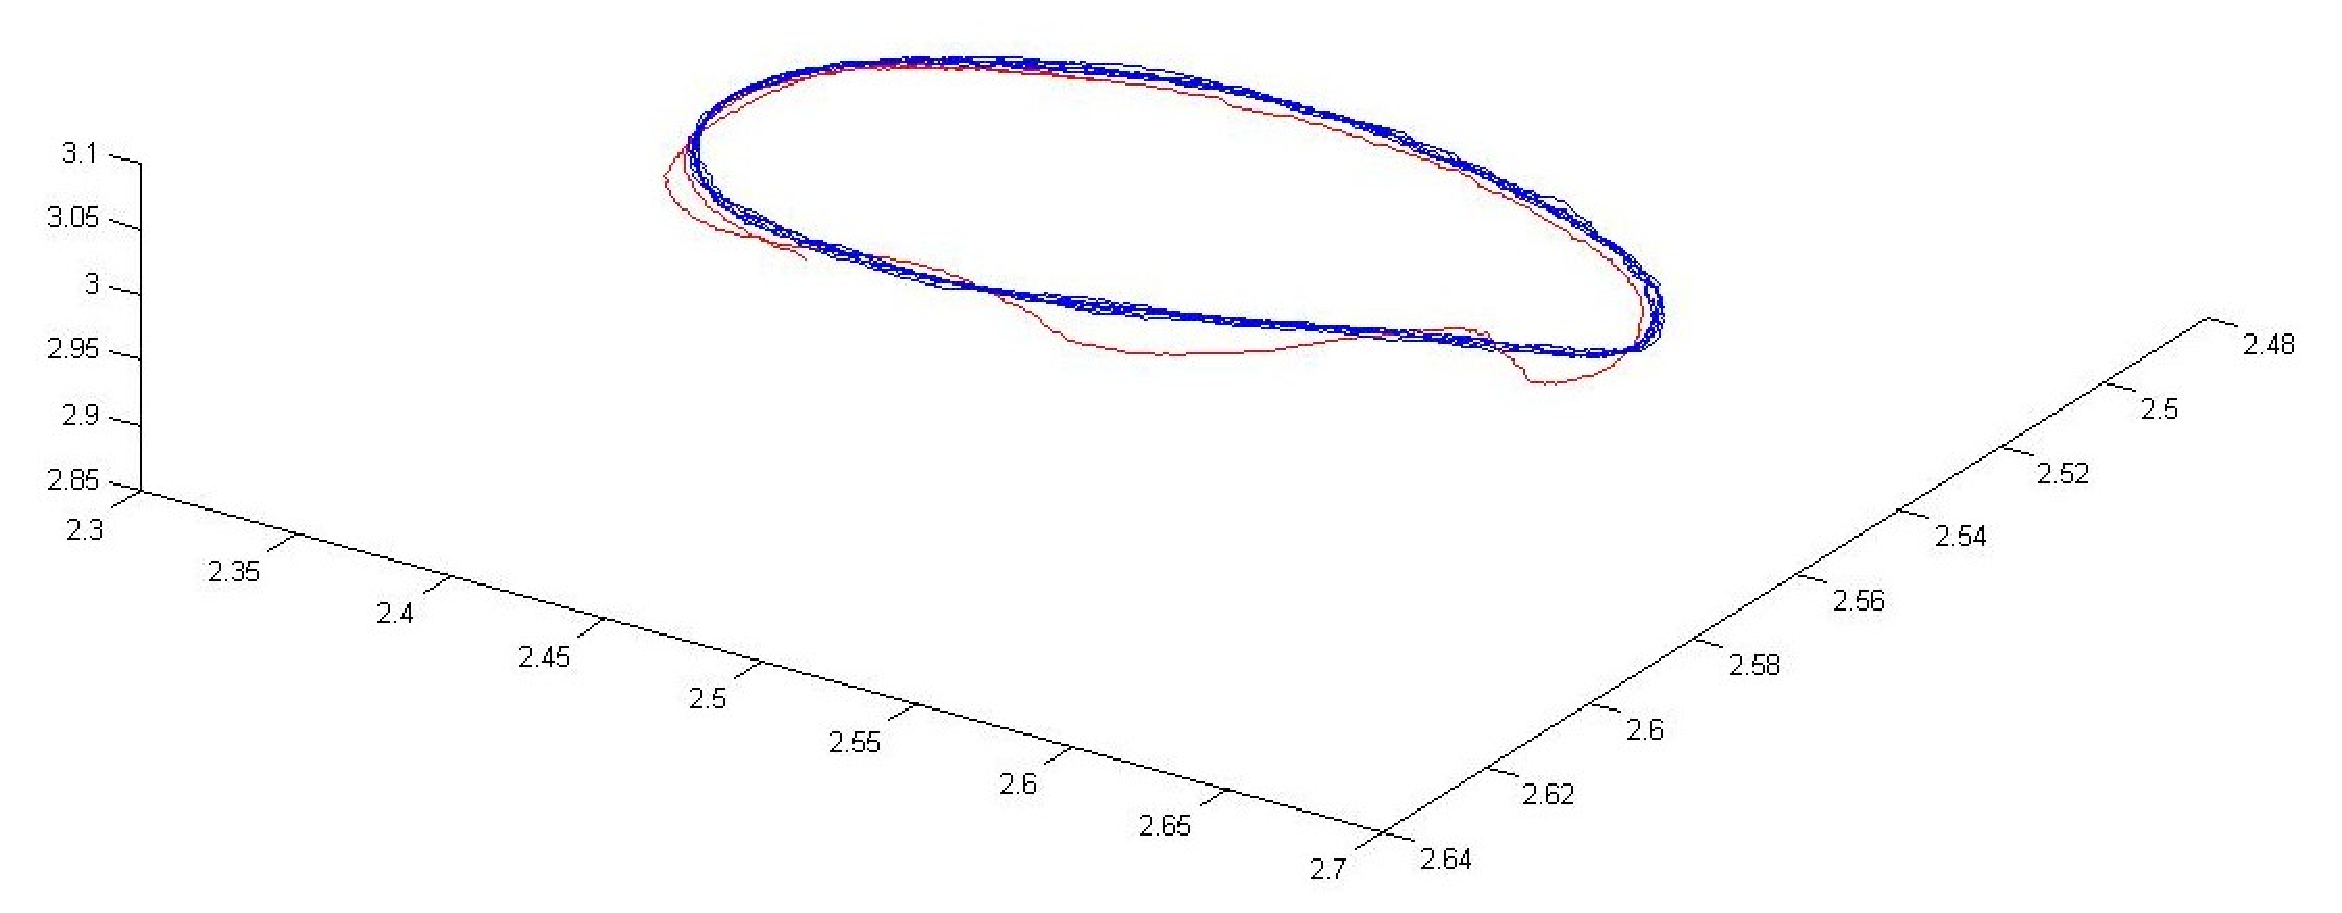
\psfig{file=figures/tam_uniform_field.eps,width=0.8\textwidth}}
  \caption{TAM measurements in a uniform field}
  \label{fig:TAMUniformField}
\end{figure}

Since the gyroscope and accelerometers were determined to be useless for the observer based controller, and the course sun sensors only able to detect motion about the z-axis, the triple-axis magnetometer remained the only sensor onboard that had the capability of detecting the nutation required for the MMS controller.

The baseline path established for TableSat in the absence of nutation (Fig fig:TAMUniformField) should be able to be compared to readings during a live run of the system and any offsets used to quantify nutation.  The same process of rotating the TableSat under a constant thrust was repeated four more times.  Each time a 200g brass weight was placed on the TableSat's deck at each principle axis $+x, +y, -x, -y$ causing the TableSat to pivot about 14 degrees out of the spin plane which was about the extent its range for nutation.  The TAM voltages for each run are grouped by color and shown in Figure \ref{fig:TAMNutationVoltages}.  Although the paths intersect and measurements are not $1:1$ to the TableSat's orientation, there is at least a separation in paths.  Further study found that while the TAM voltages are duplicated between nutation paths, points that occupy the same space in the TAM measurement have different yaw measurements as measured by the course sun sensor.

\begin{figure}[H]
  \centerline{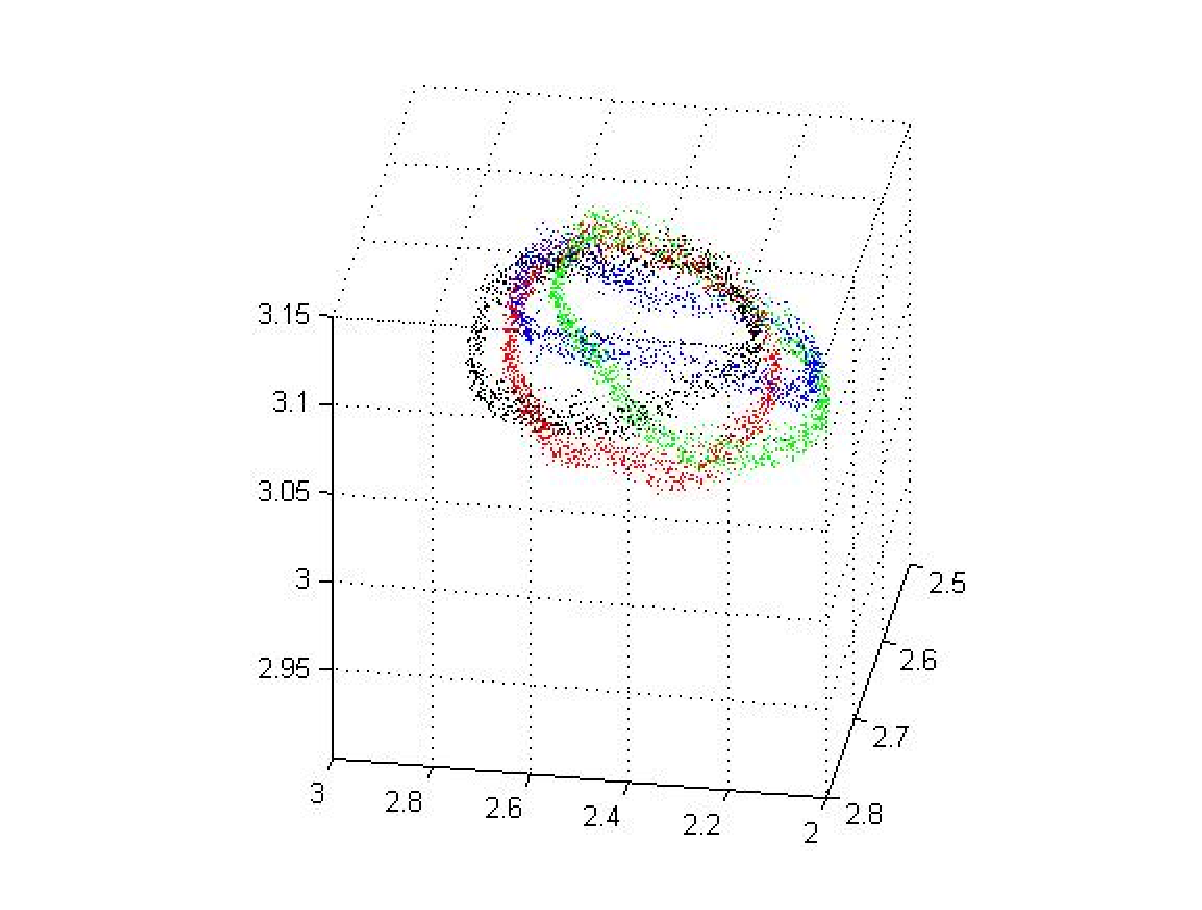
\psfig{file=figures/tam_distinct_tilts_with_good_field.eps,height=4in}}
  \caption{TAM nutation voltages}
  \label{fig:TAMNutationVoltages}
\end{figure}

\section{TableSat State Measurement}
\label{subsec:StateMeasurement}

As covered in the sections above, the only sensors available for state measurement of TableSat 1A for the observer based controller were the course sun sensor and the triple axis magnetometer.  Both of which individually measure a portion of the system's attitude and leave the system's body rate unmeasured.

Combining the measurements of the course sun sensor and triple axis magnetometer provided high confidence in the yaw measurement and rough estimates about the roll and pitch nutations.  An algorithm was developed that started with the course sun sensor and through equation \ref{eqn:CSSResultantForce} produced a measurement of yaw.  The TAM calibration data was synthesized to create a reference table of TAM readings at each of the five paths (steady, and the four nutations shown in Figure \ref{fig:TAMNutationVoltages}).  This reference table along with the equation to determine yaw from the course sun sensor are comined through a method descibed in \ref{subsec:SampleAttitudeCalculation} to approximate the TableSat's attitude.

\begin{table}[H]
  \centering
  \begin{tabular}{c|ccc|ccc}
    \hline
    Yaw   & & Steady & & & $+X \ 14^o$ & \\ \hline
    (deg) & $TAM_x$ (V) & $TAM_y$ (V) & $TAM_x$ (V) & $TAM_x$ (V) & $TAM_y$ (V) & $TAM_x$ (V)  \\ \hline
    0 & $S_{x0}$ & $S_{y0}$ & $S_{z0}$ & $+X_{x0}$ & $+X_{y0}$ & $+X_{z0}$ \\ \hline
    1 & $S_{x1}$ & $S_{y1}$ & $S_{z1}$ & $+X_{x1}$ & $+X_{y1}$ & $+X_{z1}$ \\ \hline
    ... & & & & & &  \\ \hline
    Yaw   & & $+Y \ 14^o$ & & & $-X \ 14^o$ & \\ \hline
    (deg) & $TAM_x$ (V) & $TAM_y$ (V) & $TAM_x$ (V) & $TAM_x$ (V) & $TAM_y$ (V) & $TAM_x$ (V)  \\ \hline
    0 & $+Y_{x0}$ & $+Y_{y0}$ & $+Y_{z0}$ & $-X_{x0}$ & $-X_{y0}$ & $-X_{z0}$ \\ \hline
    1 & $+Y_{x1}$ & $+Y_{y1}$ & $+Y_{z1}$ & $-X_{x1}$ & $-X_{y1}$ & $-X_{z1}$ \\ \hline
    ... & & & & & &  \\ \hline
    Yaw   & & $-Y \ 14^o$ & &  \\ \hline
    (deg) & $TAM_x$ (V) & $TAM_y$ (V) & $TAM_x$ (V)  \\ \hline
    0 & $-Y_{x0}$ & $-Y_{y0}$ & $-Y_{z0}$  \\ \hline
    1 & $-Y_{x1}$ & $-Y_{y1}$ & $-Y_{z1}$  \\ \hline
    ... & & & & & &  \\ \hline
  \end{tabular}
  \caption{TAM calibration reference table}
  \label{tbl:TAMCalibration}
\end{table}

\subsection{Sample Attitude Calculation}
\label{subsec:SampleAttitudeCalculation}

This example will go through a sample calculation of the nutation based on a single set of course sun sensor and triple axis magnetometer voltage measurements.

\subsubsection{Scan Sensor Voltages}

The base station submits message id 20 to TableSat which responds with a message 63 with a payload containing 15 floats (timestamp, 6 photodiodes, 4 accelerometrs, gyroscope, and 3 triple-axis magnetometer).

\subsubsection{Calculate Yaw From Course Sun Sensor}

Using sample CSS voltages from the photodiodes of 0.37247, 0.30899, 1.18370, 2.40020, 1.80500, and 0.44052.  The TSatPy python package whose development is detailed in Chapter \ref{chap:TSatPy} uses equation \ref{eqn:CSSResultantForce} to convert the sensor voltages into a meaningful state.

\begin{singlespace}
  \begin{minted}[mathescape,
               linenos,
               numbersep=10pt,
               frame=lines,
               framesep=2mm]{python}
import TSatPy
import numpy as np

css_v = [0.37247, 0.30899, 1.18370, 2.40020, 1.80500, 0.44052]

pda = TSatPy.Sensor.PhotoDiodeArray()
pda.update_state(css_v)
vector, radians = pda.x.q.to_rotation()

print "A %g radian (%d degree) rotation about <%g, %g, %g>" % (
    radians, radians / np.pi * 180,
    vector[0,0], vector[1,0], vector[2,0])

# Prints out
# A 3.34585 radian (191 degree) rotation about <-0, -0, -1>
  \end{minted}
  % \nocite{minted}
\end{singlespace}

\subsubsection{Create Calibration TAM Data}

About 1020 data points per calibration set
Average of 37 data points per degree




\section{Messages Between TableSat and the Base Station}


\subsection{Message Protocol}
\label{subsec:UDPTCP}

Communication between the controller and the experimental TableSat is negotiated over a User Datagram Protocol (UDP) socket.  Both the controller and TableSat read and write over port 9877.  UDP is used for a stateless connection more generally used for pushing data over a large number of connections.  The other common communication protocol is Transmission Control Protocol (TCP) where a session is established between server and client and successful transferral of data is acknowledged by the recipient.

Advantages and disadvantages exist between the TCP and UDP protocols and became a critical factor in influencing the design of TableSat 1A base station controller. Section \ref{sec:Simulink} goes into further detail in how this difference in protocols cropped up early in the development of the base station controller where the combination of Matlab Simulink with a UDP communication protocol produced a very fragile system.

A UDP message transmission is done in a ``fire and forget'' fashion.  The message header can generally include the originating hosts ip address and port so that the server knows where to send the response.  The session-less nature of UDP means that the originating server sends the message, but does not receive confirmation that the message transmitted successfully as with TCP where ever interaction is followed up with an acknowledgment from the other host.

The advantage to using UDP for the UNH TableSat 1 is that the satellite side code could be largely based off of Melissa Vess' work on her TableSat thesis where the control loop was implemented on-board, and the UDP connection was used to infrequently poll for data or modify sensor calibration values.  The UDP connection has the slight advantage of being able to transmit and receive packets without needing to wait for acknowledgments.  This could save a small fraction of time, but on modern hardware and with the small bandwidth usage this advantage is negligible.

Disadvantages to a UDP implementing the control interface through UDP include the possibility of packet loss where the sender submits a packet, but it gets corrupted or dropped.  Since UDP is a stateless connection, the sender doesn't wait for an acknowledgment which in this case would not come. This issue is handled by the communications module.  If the control loop rate on both updating the actuator voltages and polling sensor data is fast enough, a dropped packet would not matter much since a new updated set of values would be soon to follow.  Issues could be caused if the completion of a code loop was dependent on a packet coming in.  If dropped, the control loop could block until the next packet is received.  This was one issue encountered in the project version [sec:ControlLoopinSimulink].


\subsection{Message Definitions}
\label{subsec:MessageDefinitions}


The packet structure used for this project is the same as used by Melissa Vess \cite{vessthesis}. Each UDP packet is comprised of a packet header and data payload.  The packet header format remains constant for all messages containing five octets of data.

\begin{table}[H]
  \centering
  \begin{tabular}{| l | l |}
    \hline
    Header Octet & Description \\ \hline
    h1 & Message Number (0 to 255) \\ \hline
    h2 & Flags (0 - 255) \\ \hline
    h3 & Message Size (0 - 255) \\ \hline
    h4 & Message Size (0 - 255) \\ \hline
    h5 & 0 \\ \hline
  \end{tabular}
  \caption{UDP message headers}
  \label{tbl:UDPMessageHeaders}
\end{table}

The first octet (h1) contains the message number that matches to a predefined list of messages known by both the sender and recipient.  This is used to specify how the data in the payload is to be used.

The second octet (h2) is reserved for flags.  For some messages, flags can be set for additional data.  These are not used in the final implementation of UNH TableSat 1A.

The third (h3) and fourth (h4) header octets define the size of the data's payload, so when reading data in from a buffer, the header can inform the recipient how many bytes need to get read in from the buffer in order to get to the end of the packet.  For payloads less than 256 bytes only the fourth header byte is needed.  For payloads larger than 255 bytes the following formula is used to specify the message size headers.

\begin{subequations}
  \begin{align}
    h4 &= mod(size, 256) \\
    h3 &= floor(size / 256)
  \end{align}
  \label{eqn:UDPSizeHeader}
\end{subequations}

The only meta data provided along with the payload beyond the data's size is an 8 bit message number.  Both UNH TableSat 1A and the control station have identical message list definitions.

\begin{table}[H]
  \centering
  \begin{tabular}{|l|l|l|l|}
    \hline
    Message Id & Payload Size & Data Type & Message Description \\ \hline
    2 & 1 octet & unsigned int & Set run mode \\ \hline
    4 & 1 octet & unsigned int & Set run mode \\ \hline
    18 & 4 x (8 octets) & float & Set fan speed \\ \hline
    19 & 1 octet & unsigned int & Set log record mode \\ \hline
    20 & 1 octet & unsigned int & Request sensor reading \\ \hline
    22 & 1 octet & unsigned int & End of sensor log \\ \hline
    23 & 8 octets & float & Request sensor log data \\ \hline
    33 & 8 octets & float & Set log sample rate \\ \hline
    63 & 15 x (8 octets) & float & Sensor readings \\ \hline
    64 & 16 x (8 octets) & float & Sensor log entry \\ \hline
    65 & 8 octets & float & Sensor log size \\ \hline
    104 & 1 octet & unsigned int & Ack run mode \\ \hline
    118 & 1 octet & unsigned int & Ack fan volt \\ \hline
    119 & 1 octet & unsigned int & Ack sensor log run mode \\ \hline
    133 & 1 octet & unsigned int & Ack log sample rate \\ \hline
  \end{tabular}
  \caption{TableSat message definitions}
  \label{tbl:UDPMessageDefinitions}
\end{table}


\chapter{TABLESAT ATTITUDE SOFTWARE IMPLEMENTATION}
\label{chap:TableSatAttitudeDynamicsSoftware}

This chapter covers the software implementation of the attitude dynamics and control systems.  Although multiple versions of the software are created as is discussed in Chapters \ref{chap:ProgressionOfControlSystemSoftware} and \ref{chap:UNHTableSat1A}, the samples shown here are use cases of the TSatPy implementation.

\section{Implementation of Attitude Modeling}
\label{sec:ImplementationofAttitudeModeling}


\subsection{Quaternion Notation}
\label{subsec:Implementation-QuaternionNotation}

Defining a rotational quaternion using the TSatPy avoids a common issue with quaternion use where the scalar component can be placed at the leading or trailing end of the tensor depending on the author's discretion.  As is described more in Chapter \ref{chap:TSatPy}, the implementation in this thesis is done in an object oriented manner so it can handle either the scalar first or scalar last format.

\begin{singlespace}
  \begin{minted}[mathescape,linenos,numbersep=10pt,frame=lines,framesep=2mm]{python}
from TSatPy.State import Quaternion
q = Quaternion(vector=[1,2,3], scalar=4)
print(q)
q = Quaternion(scalar=0, vector=[1,2,3])
print(q)

# Prints Out
# <Quaternion [1 2 3], 4>
# <Quaternion [1 2 3], 0>
  \end{minted}
  \nocite{minted}
\end{singlespace}

\section{Rotational Quaternion}
\label{sec:Implementation-RotationalQuaternion}

The rotational quaternion is chosen as the attitude parametrization of the state vector.  As such, the two properties required to define a rotational quaternion are the Euler axis of rotation $\bs{\hat{e}}$ and the angle of rotation $\theta$.  Snippet \ref{code:make_quat_rot} demonstrates the creation of a rotational quaternion.  It also shows that proper normalization of the quaternion occurs to ensure accurate calculations.

\begin{listing}[H]
\begin{singlespace}
  \begin{minted}[mathescape,linenos,numbersep=10pt,frame=lines,framesep=2mm]{python}
from TSatPy.State import Quaternion

q = Quaternion(vector=[1,2,3], radians=4)
e, theta = q.to_rotation()

print(q)
print("Euler axis: <%g, %g, %g>" % (e[0,0], e[1,0], e[2,0]))
print("Rotation: %g radians" % theta)

# Prints Out
# <Quaternion [-0.24302 -0.48604 -0.72906], -0.416147>
# Euler axis: <-0.267261, -0.534522, -0.801784>
# Rotation: 4 radians
  \end{minted}
  \nocite{minted}
\caption{Creating a rotational quaternion}
\label{code:make_quat_rot}
\nocite{minted}
\end{singlespace}
\end{listing}

\subsection{Quaternion Multiplication}
\label{subsec:Implementation-QuaternionMultiplication}

Propagating a quaternion state accurately requires the use of the quaternion multiplication defined in \ref{eqn:QuaternionMultiplicationDerived}.  TSatPy achieves this by overriding the normal multiplication infix operator ``*''.  Snippet
\ref{code:quat_mul} demonstrates how a quaternion created from a 2 radian rotation represents the same attitude as the product of four 0.5 radian quaternions.

\begin{listing}[H]
\begin{singlespace}
  \begin{minted}[mathescape,linenos,numbersep=10pt,frame=lines,framesep=2mm]{python}
from TSatPy.State import Quaternion

a = Quaternion([1,2,3], radians=0.5)
b = Quaternion([1,2,3], radians=2)
print("a             = %s" % a)
print("a * a * a * a = %s" % (a * a * a * a))
print("b             = %s" % b)
# Prints Out
# a             = <Quaternion [-0.0661215 -0.132243 -0.198364], 0.968912>
# a * a * a * a = <Quaternion [-0.224893 -0.449785 -0.674678], 0.540302>
# b             = <Quaternion [-0.224893 -0.449785 -0.674678], 0.540302>
  \end{minted}
  \nocite{minted}
\caption{Quaternion multiplication}
\label{code:quat_mul}
\nocite{minted}
\end{singlespace}
\end{listing}

Snippet \ref{code:quat_mul_source} shows the implementation of the quaternion multiplication which reads and is used similarly to how the quaternion algebra is written.

\begin{listing}
\begin{singlespace}
  \begin{minted}[mathescape,linenos,numbersep=10pt,frame=lines,framesep=2mm]{python}
class Quaternion(object):
    def __mul__(self, q):
        v = (self.x + np.eye(3) * self.scalar) * q.vector
        v += self.vector * q.scalar
        s = self.scalar * q.scalar - (self.vector.T * q.vector)[0, 0]
        return Quaternion(v, s)
  \end{minted}
\caption{Quaternion multiplication method}
\label{code:quat_mul_source}
\nocite{minted}
\end{singlespace}
\end{listing}


\subsection{Rotating a Point with Quaternions}
\label{subsubsec:RotatingaPointwithQuaternions}

One of the main focal points of this thesis is to ensure that the tools developed in this research aide in the further development of observer-based attitude control.  To enable this goal, ``run-time'' analysis of the system is critical.  Waiting for the completion of a simulation or experimental test with TableSat IA before being able to access the information is not only an impedance to this end, but it also introduces complexity and higher ``run-time'' costs to collect and store all simulation/experimental data.  Watching representation of the system's state change as the experiment runs provides valuable insight.  In the case of an estimator, sensor voltages are converted to a measured state and the observer attempts to use it to estimate the true state of the system.  A valuable visualization is both the measured and estimated states displayed in wireframe so the effectiveness of the estimator can be readily observed.  The points in a wireframe model of TableSat can be rotated to show the estimated orientation through the use of a 3x3 rotation matrix $\bs{R}_q$ defined as
\begin{equation}
  \bs{R}_q = (q_0^2 - \bs{v}^T \bs{v}) \bs{I} + 2 \bs{v} \bs{v}^T - 2 q_0 (\bs{v} \times)
  \label{eqn:RotationMatrix}
\end{equation}

For example, for a $\pi/2$ radian rotation about $\bs{\hat{e}} = 0\bs{i}+0\bs{j}+1\bs{k}$, the rotational quaternion as defined in Equation (\ref{eqn:RotationalQuaternionDefinition}) becomes $q = 0\bs{i}+0\bs{j}-1/\sqrt{2}\bs{k}+1/\sqrt{2}$.  With Equation (\ref{eqn:RotationMatrix}), the rotational matrix becomes

\begin{equation}
  \begin{aligned}
    \bs{R_q} & = \left[ (1/\sqrt{2})^2 - (1/\sqrt{2})^2 \right] \bs{I} + 2 \begin{bmatrix} 0 & 0 & 0 \\ 0 & 0 & 0 \\ 0 & 0 & 1/\sqrt{2} \end{bmatrix} - 2 \frac{1}{\sqrt{2}} \begin{bmatrix} 0 & 1/\sqrt{2} & 0 \\ -1/\sqrt{2} & 0 & 0 \\ 0 & 0 & 0 \\ \end{bmatrix} \\
      & = \begin{bmatrix} 0 & -1 & 0 \\ 1 & 0 & 0 \\ 0 & 0 & 1 \\\end{bmatrix}
  \end{aligned}
\end{equation}

For the visualization, a point $A (2, 4, -1)$ that is in the standard orientation of body axes aligned with the global reference frame can be drawn at the current estimated location.  That is,

\begin{equation}
  A' = \bs{R_q} A = \begin{bmatrix} 0 & -1 & 0 \\ 1 & 0 & 0 \\ 0 & 0 & 1 \\\end{bmatrix} \begin{bmatrix} 2 \\ 4 \\ -1 \end{bmatrix} = \begin{bmatrix} -4 \\ 2 \\ -1 \end{bmatrix}
\end{equation}

The equivalent TSatPy implementation of the point rotation equation (Equation (\ref{eqn:RotationMatrix}))
\begin{singlespace}
  \begin{minted}[mathescape,linenos,numbersep=10pt,frame=lines,framesep=2mm]{python}
from TSatPy.State import Quaternion
import numpy as np

A = np.mat([2, 4, -1]).T
q = Quaternion([0,0,1], radians=np.pi/2)

print(q.rmatrix * A)

# Prints out
# [[-4.]
#  [ 2.]
#  [-1.]]
  \end{minted}
  \nocite{minted}
\end{singlespace}


\subsection{Quaternion-based Attitude Visualization}
\label{subsubsec:QuaternionbasedAttitudeVisualization}

% One of the largest challenges with running both simulations and live control models is having access to meaningful representations of how the system is performing.  NSS simulations are generally performed through either running of m-file scripts and analyzing logged data in a batch format after the run, or using a NSS to produce line plots of values tracked during the simulation run.


The method for calculating the new position of a point from an initial position can be extended to a collection of points that create a wireframe for the TableSat model.  Once this base wireframe is defined, the estimated attitude of the system can be visualized.  That is, if the system's estimator determines that TableSat is at an attitude of $\bs{q} = -0.38\bs{i}-0.07\bs{j}+0.91\bs{k}+0.16$, for example, this is equivalent to a 161 degree rotation about the Euler axis $\bs{\hat{e}} = 0.3844\bs{i}+0.0708\bs{j}-0.9205\bs{k}$.  Figure \ref{fig:TSatWireframe} shows the TableSat wireframe in its default configuration with its body axes aligned with the global reference frame.  The red dashed line represents the axis of rotation.

% Ideally, generating and updating a rendered model of the system at simulation time can improve the ability to attain the desired system behavior.

\begin{figure}[H]
  \centerline{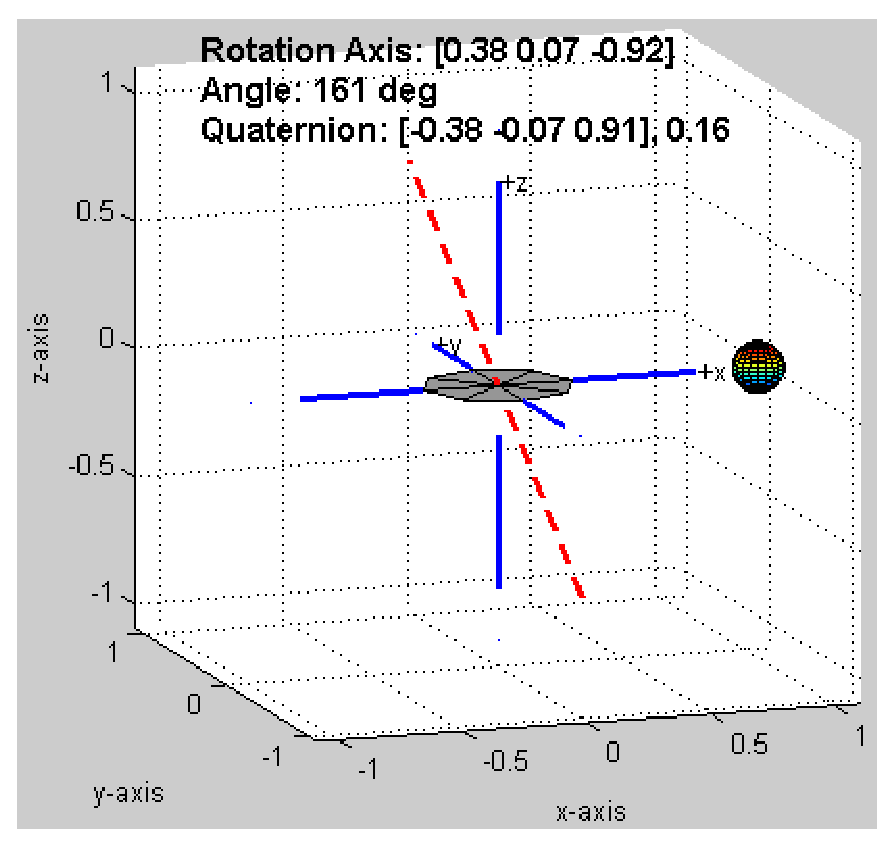
\psfig{file=figures/q_rotation_start.eps,height=3in}}
  \caption{TableSat Wireframe}
  \label{fig:TSatWireframe}
\end{figure}

Once new locations for all points in the wireframe are determined, it can be redrawn visualizing the estimated current orientation of the TableSat.  Figure \ref{fig:TSatWireframeEstimatedAttitude} shows the rotated wireframe along with the path of the body-fixed $+x$-axis traced in green.  ``Run-time'' visualizations update these representations as the simulation or experiment is occuring and shows how well the estimator runs dynamically. (discussed in greater detail in Section \ref{sec:ObjectOrientedNSSControlSystem})

\begin{figure}[H]
  \centerline{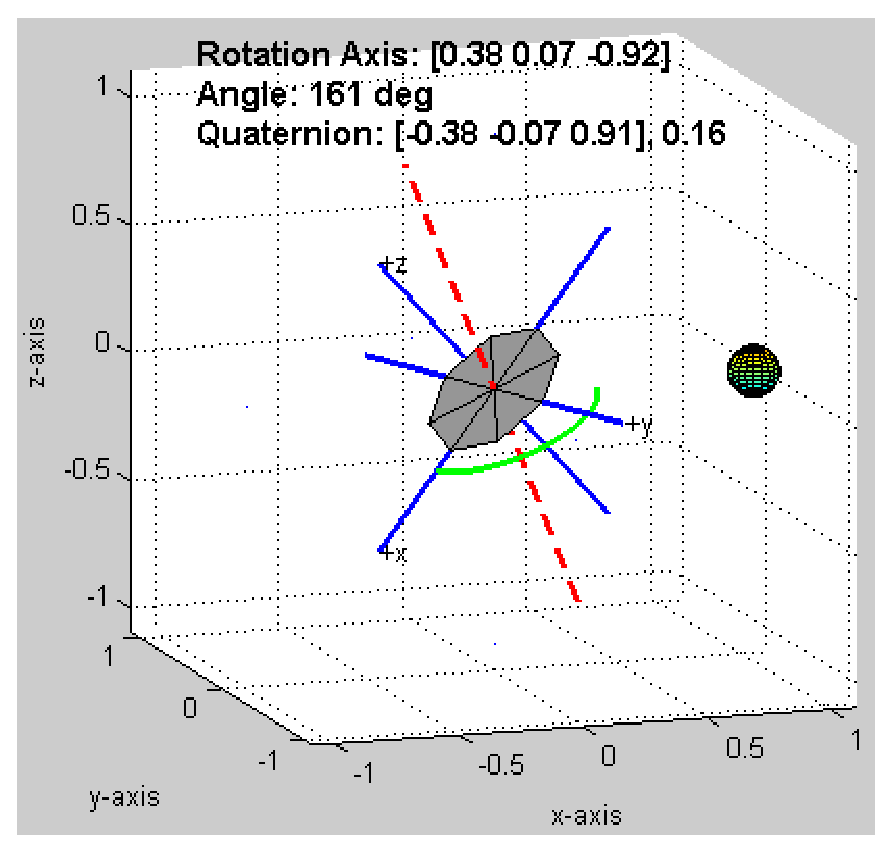
\psfig{file=figures/q_rotation_end.eps,height=3in}}
  \caption{TableSat Wireframe Estimated Attitude}
  \label{fig:TSatWireframeEstimatedAttitude}
\end{figure}


\subsection{Incremental Quaternion Rotations}
\label{subsubsec:IncrementalQuaternionRotations}

The quaternion's definition based on Euler's theorem of a rotation about a single axis simplifies the process of tracking the orientation of a spin-stabilized satellite.  NASA's MMS spacecraft has a mission spin rate of 3 rpm (~0.314 rad/sec).  A rotational quaternion, $\bs{q}_{rps}$, representing the per second rotation about the z-axis is

\begin{equation}
  \begin{aligned}
    \bs{q}_{rps} = & ( 0\bs{i} + 0\bs{j} + 1\bs{k} ) \sin \left( \frac{-0.314}{2} \right) + \cos \left( \frac{-0.314}{2} \right) \\
    = & 0\bs{i} +0\bs{j} -0.156434\bs{k} + 0.987688
  \end{aligned}
\end{equation}

In an open loop system, the best prediction of the state is to apply the quaternion rotation at each second to the previous steps state prediction, and the prediction is initialized with a known orientation.  For example, if TableSat performs a $+1/4$ turn about the z-axis each second, the best prediction at the current attitude can be obtained using just a quaternion multiplication as follows

\begin{equation}
  \begin{aligned}
    \bs{q}(t_{k+1}) = & \bs{q}_{rps} \otimes \bs{q}(t_{k}) \\
    \text{where } \bs{q}(t_0) = & 0 \bs{i} +0 \bs{j} -0.707107 \bs{k} +0.707107
  \end{aligned}
  \label{eqn:3rpmQuaternionEquation}
\end{equation}

Using the TSatPy code, Equation (\ref{eqn:3rpmQuaternionEquation}) can be implemented as

\begin{singlespace}
  \begin{minted}[mathescape,linenos,numbersep=10pt,frame=lines,framesep=2mm]{python}
from TSatPy.State import Quaternion
import time
import numpy as np

q_rps = Quaternion([0,0,1], radians=np.pi/10)
print('Quaternion spin rate (rad/sec)\n %s' % q_rps)

q_state = Quaternion([0,0,1], radians=np.pi/2)
print('Initial state of TableSat\n t=0: %s' % q_state)


print('Starting Open Loop State Tracking')
for k in range(1,11):
    time.sleep(1)
    q_state *= q_rps
    print(' t=%s: %s' % (k, q_state))

# Prints Out
# Quaternion spin rate (rad/sec)
#  <Quaternion [-0 -0 -0.156434], 0.987688>
# Initial state of TableSat
#  t=0: <Quaternion [-0 -0 -0.707107], 0.707107>
# Starting Open Loop State Tracking
#  t=1: <Quaternion [0 0 -0.809017], 0.587785>
#  t=2: <Quaternion [0 0 -0.891007], 0.45399>
#  t=3: <Quaternion [0 0 -0.951057], 0.309017>
#  t=4: <Quaternion [0 0 -0.987688], 0.156434>
#  t=5: <Quaternion [0 0 -1], 1.11022e-16>
#  t=6: <Quaternion [0 0 -0.987688], -0.156434>
#  t=7: <Quaternion [0 0 -0.951057], -0.309017>
#  t=8: <Quaternion [0 0 -0.891007], -0.45399>
#  t=9: <Quaternion [0 0 -0.809017], -0.587785>
#  t=10: <Quaternion [0 0 -0.707107], -0.707107>
  \end{minted}
  \nocite{minted}
\end{singlespace}

This method has a significant issue.  The theoretical concern is the estimate is that running in an open loop fashion without receiving correction updates.  Therefore, the myriad of additional factors in a real system would quickly invalidate the accuracy of this approach.  The implementation issue deals with the time step.  Even if TableSat spins perfectly at 3 rpm, the state is not updated exactly on each second.  A busy processor, numerical drift, and execution time would prevent the desired fixed step size of 1 sec.  In some of the earlier implementations of the base station controller (discussed in Chapter \ref{chap:ProgressionOfControlSystemSoftware}), dropped UDP messages cause the control loop to execute on an inconsistent interval and prevent accurate state estimates.  (Handling of the variability in time steps is discussed in Section \ref{sec:SatelliteDynamics})


\subsection{Quaternion Decomposition}
\label{subsec:TSatPyQuaternionDecomposition}

The need for a quaternion decomposition is noted in Section \ref{subsec:QuaternionDecompositionForNutationControl} of the controls chapter and the method for performing the decomposition is derived in \ref{subsec:QuaternionDecomposition}.  Snippet \ref{code:sample_quaternion_decomposition} shows a this functionality as built in the TSatPy software through the decomposition of a quaternion representing a 1 radian rotation about the Euler axis $[0 \ 0.1 \ 1]^T$

\begin{listing}[H]
\begin{singlespace}
  \begin{minted}[mathescape,linenos,numbersep=10pt,frame=lines,framesep=2mm]{python}
from TSatPy.State import State, Quaternion, BodyRate

print("State Error")
x_e = State(
    Quaternion([0,0.1,1],radians=1),
    BodyRate([0,-0.01,0.2]))
print("x_e: %s" % (x_e))

print("Decomposed Quaternion")
q_r, q_n = x_e.q.decompose()
print("q_r: %s" % q_r)
print("q_n: %s" % q_n)

print("Nutation Only State Error")
x_e.q = q_n
print("x_e: %s" % (x_e))

# Prints Out
# State Error
# x_e: <Quaternion [-0 -0.0477046 -0.477046], 0.877583>,
#      <BodyRate [0 -0.01 0.2]>
# Decomposed Quaternion
# q_r: <Quaternion [0 0 -0.47759], 0.878583>
# q_n: <Quaternion [-0.0227833 -0.0419125 -0], -0.998861>
# Nutation Only State Error
# x_e: <Quaternion [-0.0227833 -0.0419125 -0], -0.998861>,
#      <BodyRate [0 -0.01 0.2]>
  \end{minted}
\caption{Quaternion decomposition}
\label{code:sample_quaternion_decomposition}
\nocite{minted}
\end{singlespace}
\end{listing}




\section{Satellite Dynamics}
\label{sec:SatelliteDynamics}

One of the goals in creating an accurate dynamic model is to predict the state of the system given the last know state, the elapsed time since the last known state, and any inputs to the system.  The initial scope of predicting the satellite's state is restricting it to a state propagation problem where only last state and elapsed time are considered.  (Estimation techniques in Section \ref{chap:Estimators} describes how a propagated state can be adjusted using the measured state.)

\subsection{System Clock}
\label{subsec:SystemClock}

As mentioned previously, the chance of having perfectly timed updates is highly unlikely.  Small variations in the time step size results in errors.  A state update running every 1.0001 seconds instead of every second would accumulate over a six degree error after tracking TableSat's state for an hour.  A linearized model is also affected because the expected time step size is incorporated as part of the discretization processes.

The preset fixed time step is also not very fault tolerant.  When controlling the state of a stable, slow moving system the state, the tracking rate can be decreased to conserve system resources.  In this circumstance a missed or series of missed updates due to faults can cause the predicted state to lag by be several time steps.  A variable step sized based solution can improve the robustness against these errors.

The ability to decrease the simulation speed to enable more detailed inspection of the initial transient behavior and to increase simulation speed to enable inspection of long term system stability hold significant benefits for this research.  The TSatPy system is designed to address the previous two issues as the system needs to be able to smoothly transition between variations in step sizes in a single experimental test such that

\begin{equation}
  t_k = \sum\limits_{i=0}^{k-1} r_i (\tau_{i+1} - \tau_i)\\
  \label{eqn:SystemTime}
\end{equation}
where $\tau$ represents true time and $t_k$ denotes the time at step $k$

The system clock defined in Equation (\ref{eqn:SystemTime}) initializes at zero and increases accordingly for varying step sizes.  TSatPy implements this concept through the Metronome class as shown in Snippet \ref{code:metronome}.  An instance of this class serves as the reference frame for all rate calculations.  During the simulation, the clock is able to adjust speed according to varying set speed.

\begin{listing}[H]
\begin{singlespace}
  \begin{minted}[mathescape,linenos,numbersep=10pt,frame=lines,framesep=2mm]{python}
from TSatPy.Clock import Metronome
import time

c = Metronome()
print("Start Time: system=%s, real=%s" % (c, time.time()))
time.sleep(2)
print("Lock step:  system=%s, real=%s" % (c, time.time()))
c.set_speed(0.1)
time.sleep(30)
print("Slow-mo:    system=%s, real=%s" % (c, time.time()))
c.set_speed(100)
time.sleep(4)
print("FFW:        system=%s, real=%s" % (c, time.time()))

# Prints Out
# Start Time: system=7.86781e-06s, real=1396147884.5
# Lock step:  system=2.00162s, real=1396147886.5
# Slow-mo:    system=5.00364s, real=1396147916.52
# FFW:        system=405.292s, real=1396147920.52
  \end{minted}
\caption{Metronome}
\label{code:metronome}
\nocite{minted}
\end{singlespace}
\end{listing}


\subsection{Body Rate and Quaternion Propagation}
\label{subsec:BodyRateQuaternionPropagation}

Predicting the body rates $\omega_x, \omega_y,$ and $\omega_z$ for TableSat requires knowledge of the body dynamics, the last calculated body rate, time elapsed since last update, and any applied moments.  Equation (\ref{eqn:DiscreteEulerMomentEquations}) is used to propagate the body rate taking into account variable step sizes.

\begin{singlespace}
  \begin{minted}[mathescape,linenos,numbersep=10pt,frame=lines,framesep=2mm]{python}
from TSatPy.Clock import Metronome
from TSatPy import State
import time

clock = Metronome()

M = [0, 0, 0.5]
w = State.BodyRate([0, 0, 0])
eme = State.EulerMomentEquations(
    [[10, 0, 0], [0, 10, 0], [0, 0, 10]], w, clock)

for k in range(5):
    w = eme.propagate(M)
    print(w)
    time.sleep(1)

# Prints Out
# <BodyRate [0 0 0]>
# <BodyRate [0 0 0.0500562]>
# <BodyRate [0 0 0.10012]>
# <BodyRate [0 0 0.150189]>
# <BodyRate [0 0 0.200252]>
  \end{minted}
\nocite{minted}
\end{singlespace}

The quaternion propagation operates in the same way as the body rate propagation, and Equation (\ref{eqn:DiscreteQuaternionPropagation}) is implemented in the QuaternionDynamics (Chapter \ref{chap:tsatpy_source}).  Snippet \ref{code:quaternion_prop_clock} describes a basic quaternion propagation where the TableSat model is tracking a 0.1 rad/sec rotation about the $+z$ axis.  The system clock initially tracks in real time (e.g. a second of real elapsed time roughly equates to the equivalent system time change).  After each update the angle increases by about 0.1 rad.  After a four second transient response period, the speed of the system clock is increased by a factor of five (line 19).  After that each step simulates a 0.5 rad increase from when the clock speed changed.

\begin{listing}[H]
\begin{singlespace}
  \begin{minted}[mathescape,linenos,numbersep=10pt,frame=lines,framesep=2mm]{python}

from TSatPy.Clock import Metronome
from TSatPy import State
import time

c = Metronome()
print("Setting spin rate of 0.1 rad/sec about +z")
w = State.BodyRate([0, 0, 0.1])
q_ic = State.Identity()

qd = State.QuaternionDynamics(q_ic, c)

for _ in range(4):
    time.sleep(1)
    e, theta = qd.propagate(w).to_rotation()
    print(" Rotation Angle: %s" % theta)

print("Initial transient response inspection complete.")
print("Speed up 5x for steady state response.")
c.set_speed(5)

for _ in range(4):
    time.sleep(1)
    e, theta = qd.propagate(w).to_rotation()
    print(" Rotation Angle: %s" % theta)

# Prints Out
# Setting spin rate of 0.1 rad/sec about +z
#  Rotation Angle: 0.0
#  Rotation Angle: 0.100147199631
#  Rotation Angle: 0.203001904488
#  Rotation Angle: 0.303643703461
# Initial transient response inspection complete.
# Speed up 5x for steady state response.
#  Rotation Angle: 0.804805707932
#  Rotation Angle: 1.30787069798
#  Rotation Angle: 1.81127579212
#  Rotation Angle: 2.3147197485
  \end{minted}
\caption{Quaternion propagation with varying clock speed}
\label{code:quaternion_prop_clock}
\nocite{minted}
\end{singlespace}
\end{listing}

In this study, quaternion and body rate propagation techniques will be incorporated into the TableSat IA observer-based control system.

\section{Messages Between TableSat and the Base Station}

\subsection{Message Protocol}
\label{subsec:UDPTCP}

Communication between the controller and the experimental TableSat is negotiated over a User Datagram Protocol (UDP) socket.  Both the controller and TableSat read and write over port 9877.  UDP is used for a stateless connection more generally used for pushing data over a large number of connections.  The other common communication protocol is Transmission Control Protocol (TCP) where a session is established between server and client and successful transferral of data is acknowledged by the recipient.

Advantages and disadvantages exist between the TCP and UDP protocols and became a critical factor in influencing the design of TableSat IA base station controller. Section \ref{sec:NSSModel} goes into further detail in how this difference in protocols cropped up early in the development of the base station controller where the combination of a Numerical Simulation Software (like MATLAB Simulink or Octave) with a UDP communication protocol produced a very fragile system.

A UDP message transmission is done in a ``fire and forget'' fashion.  The message header can generally include the originating hosts ip address and port so that the server knows where to send the response.  The session-less nature of UDP means that the originating server sends the message, but does not receive confirmation that the message transmitted successfully as with TCP where ever interaction is followed up with an acknowledgment from the other host.

The advantage to using UDP for the UNH TableSat 1 is that the satellite side code could be largely based off of Melissa Vess' work on her TableSat thesis where the control loop was implemented on-board, and the UDP connection was used to infrequently poll for data or modify sensor calibration values.  The UDP connection has the slight advantage of being able to transmit and receive packets without needing to wait for acknowledgments.  This could save a small fraction of time, but on modern hardware and with the small bandwidth usage this advantage is negligible.

Disadvantages to a UDP implementing the control interface through UDP include the possibility of packet loss where the sender submits a packet, but it gets corrupted or dropped.  Since UDP is a stateless connection, the sender doesn't wait for an acknowledgment which in this case would not come. This issue is handled by the communications module.  If the control loop rate on both updating the actuator voltages and polling sensor data is fast enough, a dropped packet would not matter much since a new updated set of values would be soon to follow.  Issues could be caused if the completion of a code loop was dependent on a packet coming in.  If dropped, the control loop could block until the next packet is received.  This was one issue encountered in the project version [sec:ControlLoopinSimulink].


\subsection{Message Definitions}
\label{subsec:MessageDefinitions}


The packet structure used for this project is the same as used by Melissa Vess \cite{vessthesis}. Each UDP packet is comprised of a packet header and data payload.  The packet header format remains constant for all messages containing five octets of data.

\begin{table}[H]
  \centering
  \begin{tabular}{| l | l |}
    \hline
    Header Octet & Description \\ \hline
    h1 & Message Number (0 to 255) \\ \hline
    h2 & Flags (0 - 255) \\ \hline
    h3 & Message Size (0 - 255) \\ \hline
    h4 & Message Size (0 - 255) \\ \hline
    h5 & 0 \\ \hline
  \end{tabular}
  \caption{UDP message headers}
  \label{tbl:UDPMessageHeaders}
\end{table}

The first octet (h1) contains the message number that matches to a predefined list of messages known by both the sender and recipient.  This is used to specify how the data in the payload is to be used.

The second octet (h2) is reserved for flags.  For some messages, flags can be set for additional data.  These are not used in the final implementation of NASA MMS TableSat IA.

The third (h3) and fourth (h4) header octets define the size of the data's payload, so when reading data in from a buffer, the header can inform the recipient how many bytes need to get read in from the buffer in order to get to the end of the packet.  For payloads less than 256 bytes only the fourth header byte is needed.  For payloads larger than 255 bytes the following formula is used to specify the message size headers.

\begin{subequations}
  \begin{align}
    h4 &= mod(size, 256) \\
    h3 &= floor(size / 256)
  \end{align}
  \label{eqn:UDPSizeHeader}
\end{subequations}

The only meta data provided along with the payload beyond the data's size is an 8 bit message number.  Both UNH TableSat IA and the control station have identical message list definitions.

\begin{table}[H]
  \centering
  \begin{tabular}{|l|l|l|l|}
    \hline
    Message Id & Payload Size & Data Type & Message Description \\ \hline
    2 & 1 octet & unsigned int & Set run mode \\ \hline
    4 & 1 octet & unsigned int & Set run mode \\ \hline
    18 & 4 x (8 octets) & float & Set fan voltages \\ \hline
    19 & 1 octet & unsigned int & Set log record mode \\ \hline
    20 & 1 octet & unsigned int & Request sensor reading \\ \hline
    22 & 1 octet & unsigned int & End of sensor log \\ \hline
    23 & 8 octets & float & Request sensor log data \\ \hline
    33 & 8 octets & float & Set log sample rate \\ \hline
    63 & 15 x (8 octets) & float & Sensor readings \\ \hline
    64 & 16 x (8 octets) & float & Sensor log entry \\ \hline
    65 & 8 octets & float & Sensor log size \\ \hline
    104 & 1 octet & unsigned int & Ack run mode \\ \hline
    118 & 1 octet & unsigned int & Ack fan volt \\ \hline
    119 & 1 octet & unsigned int & Ack sensor log run mode \\ \hline
    133 & 1 octet & unsigned int & Ack log sample rate \\ \hline
  \end{tabular}
  \caption{TableSat message definitions}
  \label{tbl:UDPMessageDefinitions}
\end{table}


\section{Calculating Nutation From Three-Axis Magnetometer}

The following example shows a sample calculation of nutation based on a single set of coarse sun sensor and TAM voltage measurements.

The base station submits a request for sensor data (message id \#20) to TableSat which responds with a packet containing the sensor output voltages (message id \#63) with a payload containing 15 floats (timestamp, 6 photodiodes, 4 accelerometrs, gyroscope, and 3 three-axis magnetometer).

\subsection{Calculate Yaw From Coarse Sun Sensor}

Using sample CSS output voltages from the photodiodes (0.37247, 0.30899, 1.18370, 2.40020, 1.80500, and 0.44052), the TSatPy python package (whose development is detailed in Chapter \ref{chap:TSatPy}) uses Equation (\ref{eqn:CSSResultantForce}) to convert the sensor voltages into a meaningful state as shown in Snippet \ref{code:css_to_yaw}.

\begin{listing}[H]
\begin{singlespace}
  \begin{minted}[mathescape,
               linenos,
               numbersep=10pt,
               frame=lines,
               framesep=2mm]{python}
import TSatPy
import numpy as np

css_v = [0.37247, 0.30899, 1.18370, 2.40020, 1.80500, 0.44052]

pda = TSatPy.Sensor.PhotoDiodeArray()
pda.update_state(css_v)
vector, radians = pda.x.q.to_rotation()

print "A %g radian (%d degree) rotation about <%g, %g, %g>" % (
    radians, radians / np.pi * 180,
    vector[0,0], vector[1,0], vector[2,0])

# Prints out
# A 3.34585 radian (191 degree) rotation about <-0, -0, -1>
  \end{minted}
\caption{Converting CSS voltage outputs to a Yaw measurement}
\label{code:css_to_yaw}
\nocite{minted}
\end{singlespace}
\end{listing}

\subsection{Calculate TAM Nutation Reference Data}
\label{subsec:CalculateTAMNutationReferenceData}

Figure \ref{fig:TAMNutationVoltages} shows that while the TAM readings vary enough to be noticeable for large nutations, the signal contain a significant level of noise.  In order to use the TAM to quantify nutation for the observer-based controller, the data in Table \ref{tbl:TAMCalibration} is reduced to five data points for a yaw angle of 191 degrees.  When updating the estimator, TAM sensor values can be compared to the five reference nutation points of level, $+x$ down, $+y$ down, $-x$ down, and $-y$ down.

\begin{table}[H]
  \centering
  \begin{tabular}{c|c|c|c}
    \hline
    Yaw   & Steady & $+X \ 14^o$ & $+Y \ 14^o$ \\ \hline
    (deg) & TAM (V) & TAM (V) & TAM (V) \\ \hline
    0 & $(S_{x0},S_{y0},S_{z0})$ & $(+X_{x0},+X_{y0},+X_{z0})$ & $(+Y_{x0},+Y_{y0},+Y_{z0})$\\
    1 & $(S_{x1},S_{y1},S_{z1})$ & $(+X_{x1},+X_{y1},+X_{z1})$ & $(+Y_{x1},+Y_{y1},+Y_{z1})$\\
    2 & $(S_{x2},S_{y2},S_{z2})$ & $(+X_{x2},+X_{y2},+X_{z2})$ & $(+Y_{x2},+Y_{y2},+Y_{z2})$\\
    ... & & &  \\ \hline
    \hline
    Yaw   & $-X \ 14^o$ & $-Y \ 14^o$ \\ \hline
    (deg) & TAM (V) & TAM (V) \\ \hline
    0 & $(-X_{x0},-X_{y0},-X_{z0})$ & $(-Y_{x0},-Y_{y0},-Y_{z0})$\\
    1 & $(-X_{x1},-X_{y1},-X_{z1})$ & $(-Y_{x1},-Y_{y1},-Y_{z1})$\\
    2 & $(-X_{x2},-X_{y2},-X_{z2})$ & $(-Y_{x2},-Y_{y2},-Y_{z2})$\\
    ... & & &  \\ \hline
  \end{tabular}
  \caption{TAM calibration reference table structure}
  \label{tbl:TAMCalibration}
\end{table}

The method chosen for creating the five reference points starts with collecting approximately 2400 data points with corresponding TAM and coarse sun sensor voltage readings.  The voltages for each nutation setting are grouped into 1 degree increments.  Multiple rotations create some overlap in measurements.  The final reference value for each degree is calculated through a weighted average of a specified smoothing window.

Figure \ref{fig:TAMNutationReference} shows the result of the nutation reference values for 5, 15 and 25 degree smoothing windows.  At $\pm 15$ degrees, an adequate level of noise is filtered without causing over smoothing.  At this level, each of the 191 degree reference values are a weighted average of about 200 of the original calibration points.

\begin{figure}[H]
  \begin{subfigure}[h!]{0.8\textwidth}
    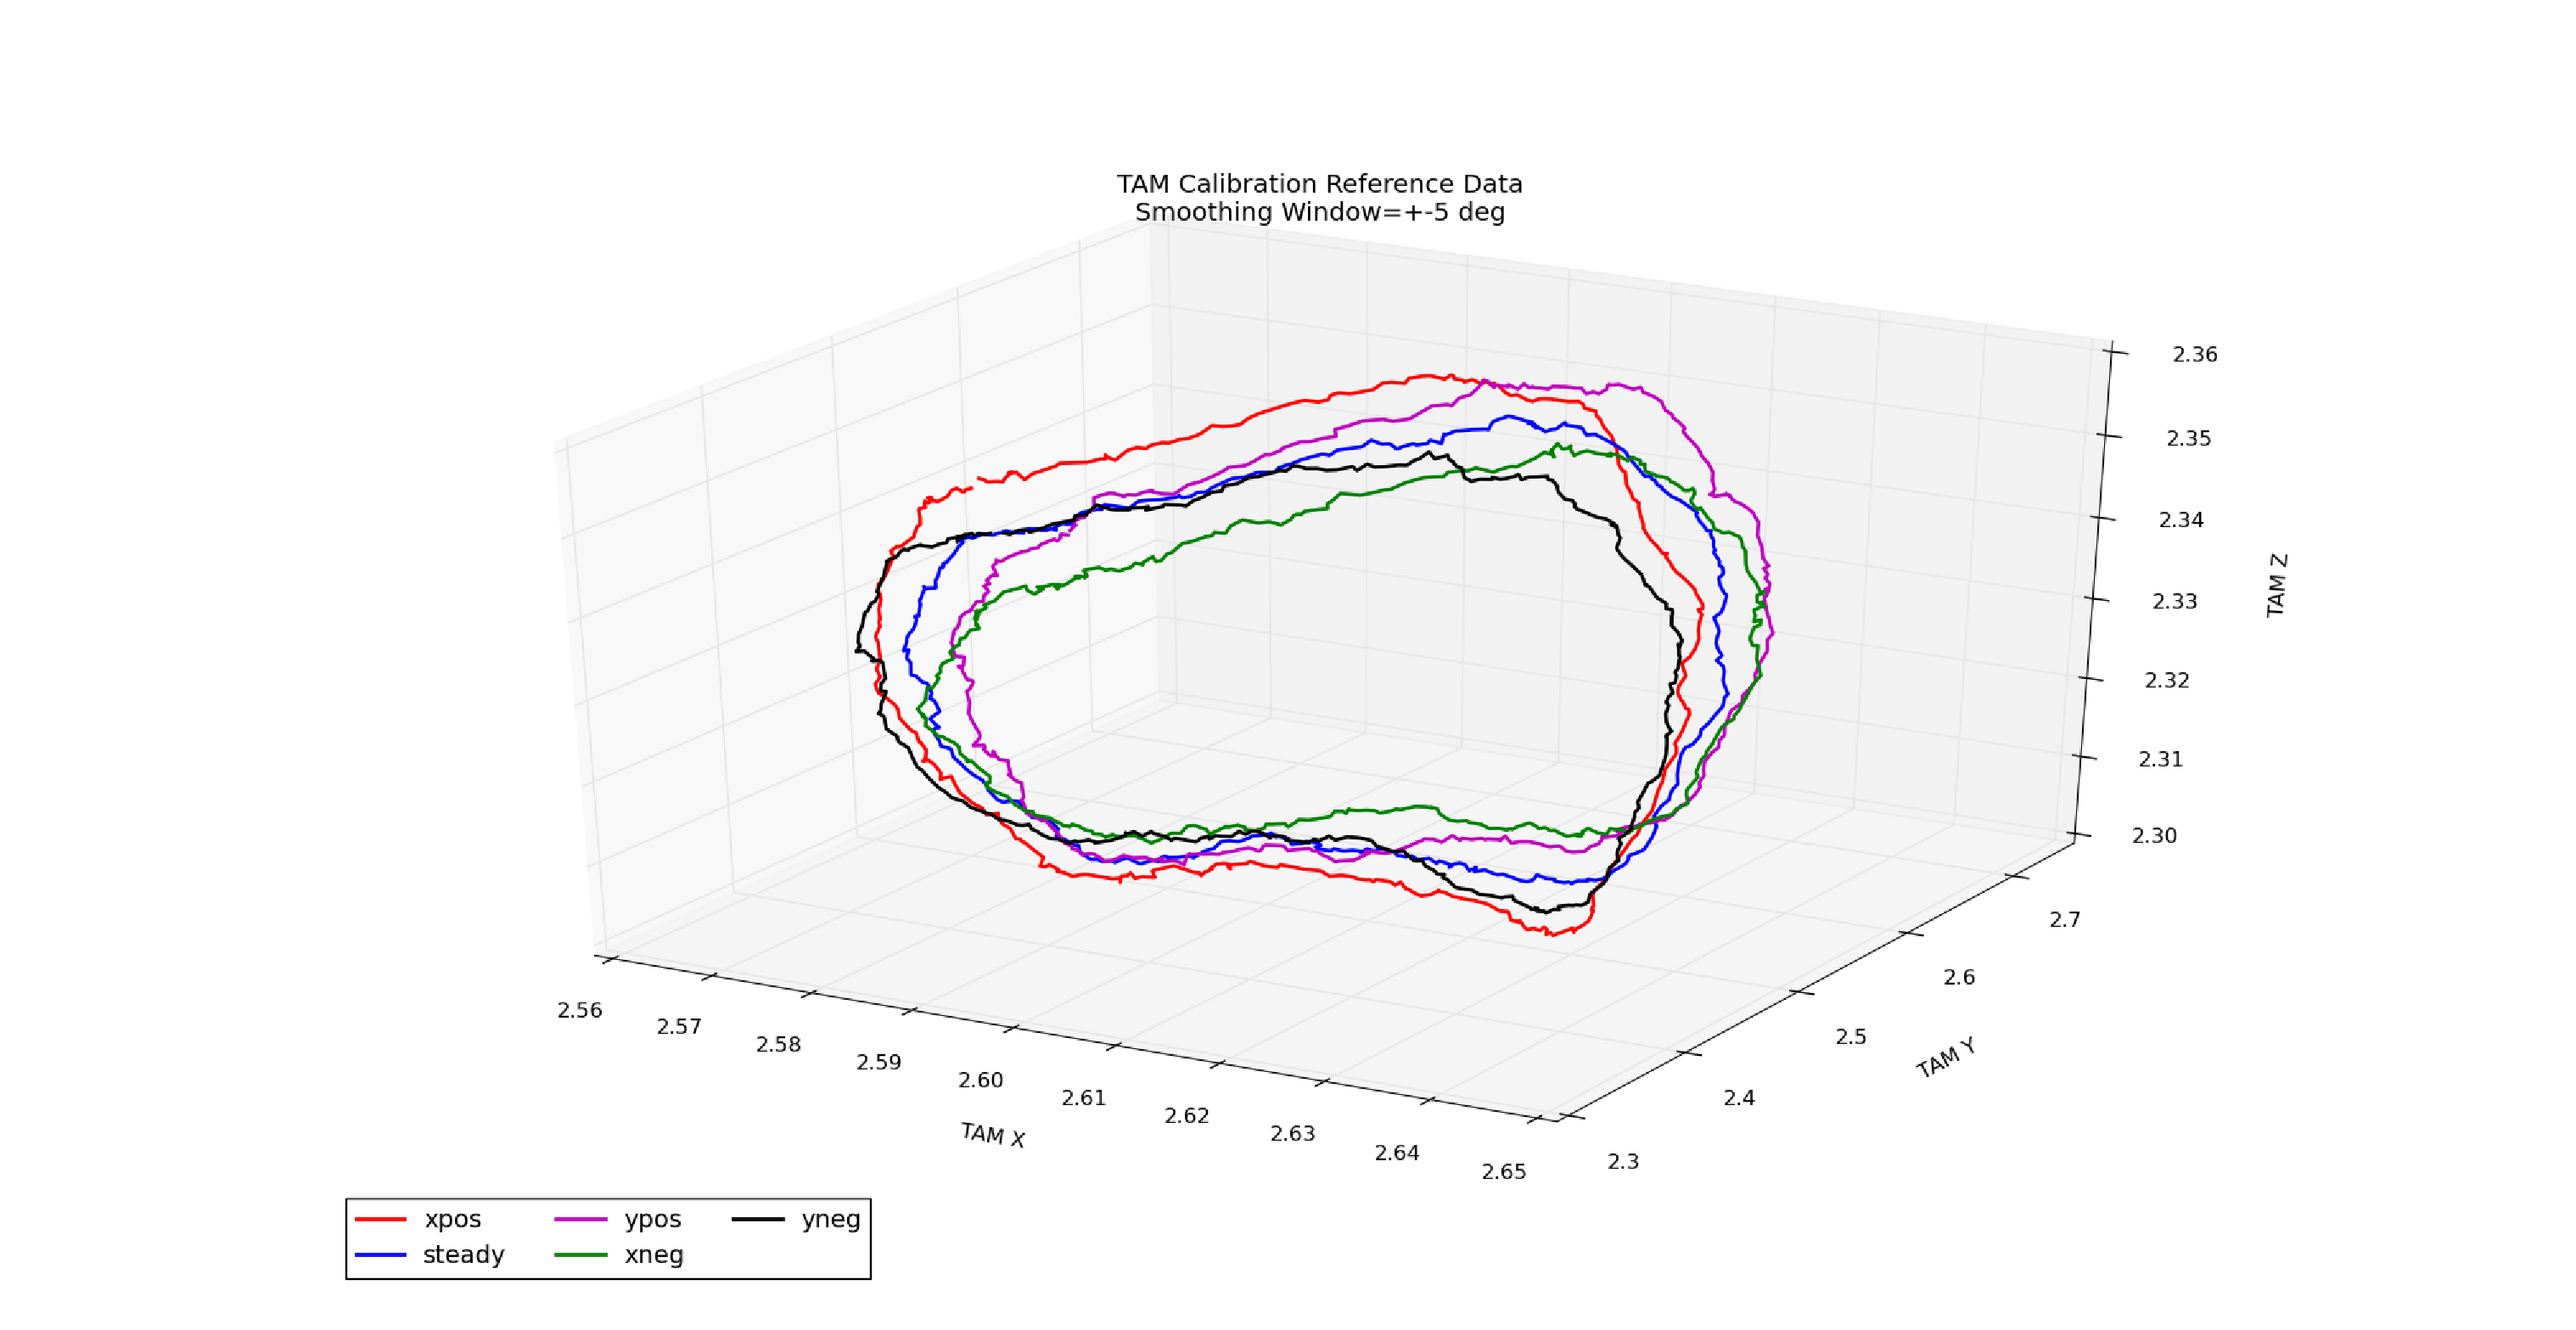
\includegraphics[width=\textwidth]{figures/tam_calibration_ref_5deg_smoothing.eps}
    \caption{$\pm 5^o$ smoothing}
    \label{fig:TAM5degCalibration}
  \end{subfigure}

  \begin{subfigure}[h!]{0.8\textwidth}
    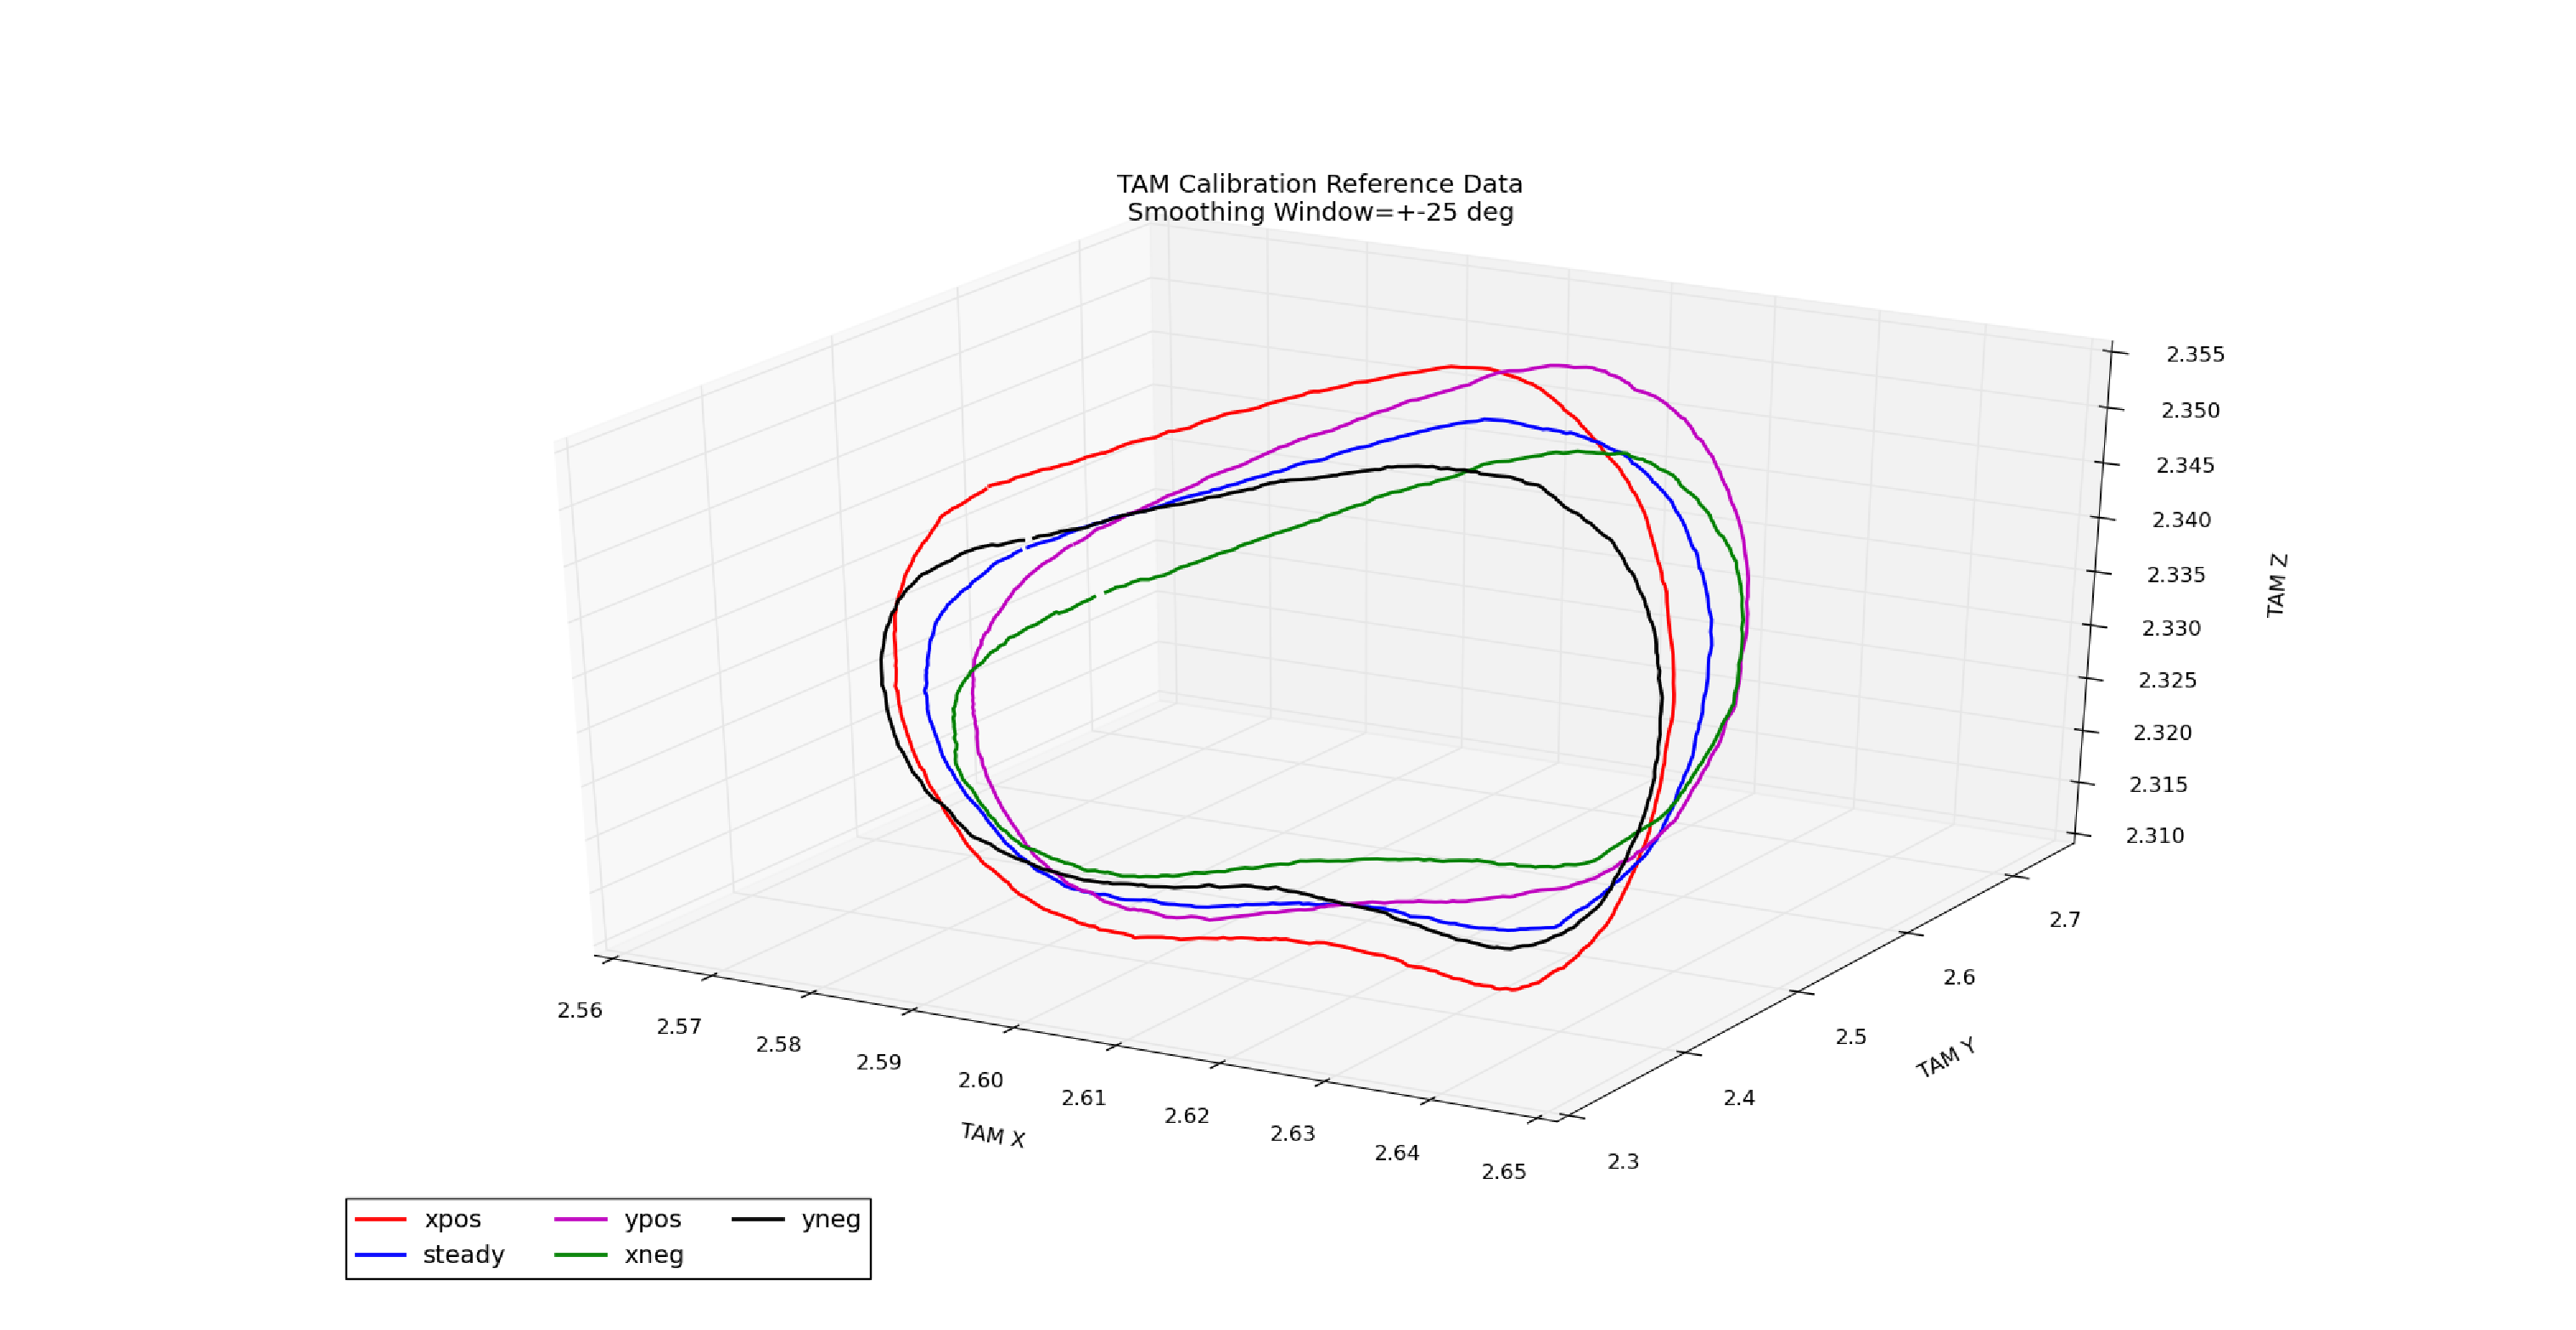
\includegraphics[width=\textwidth]{figures/tam_calibration_ref_25deg_smoothing.eps}
    \caption{$\pm 25^o$ smoothing}
    \label{fig:TAM25degCalibration}
  \end{subfigure}

  \begin{subfigure}[h!]{0.8\textwidth}
    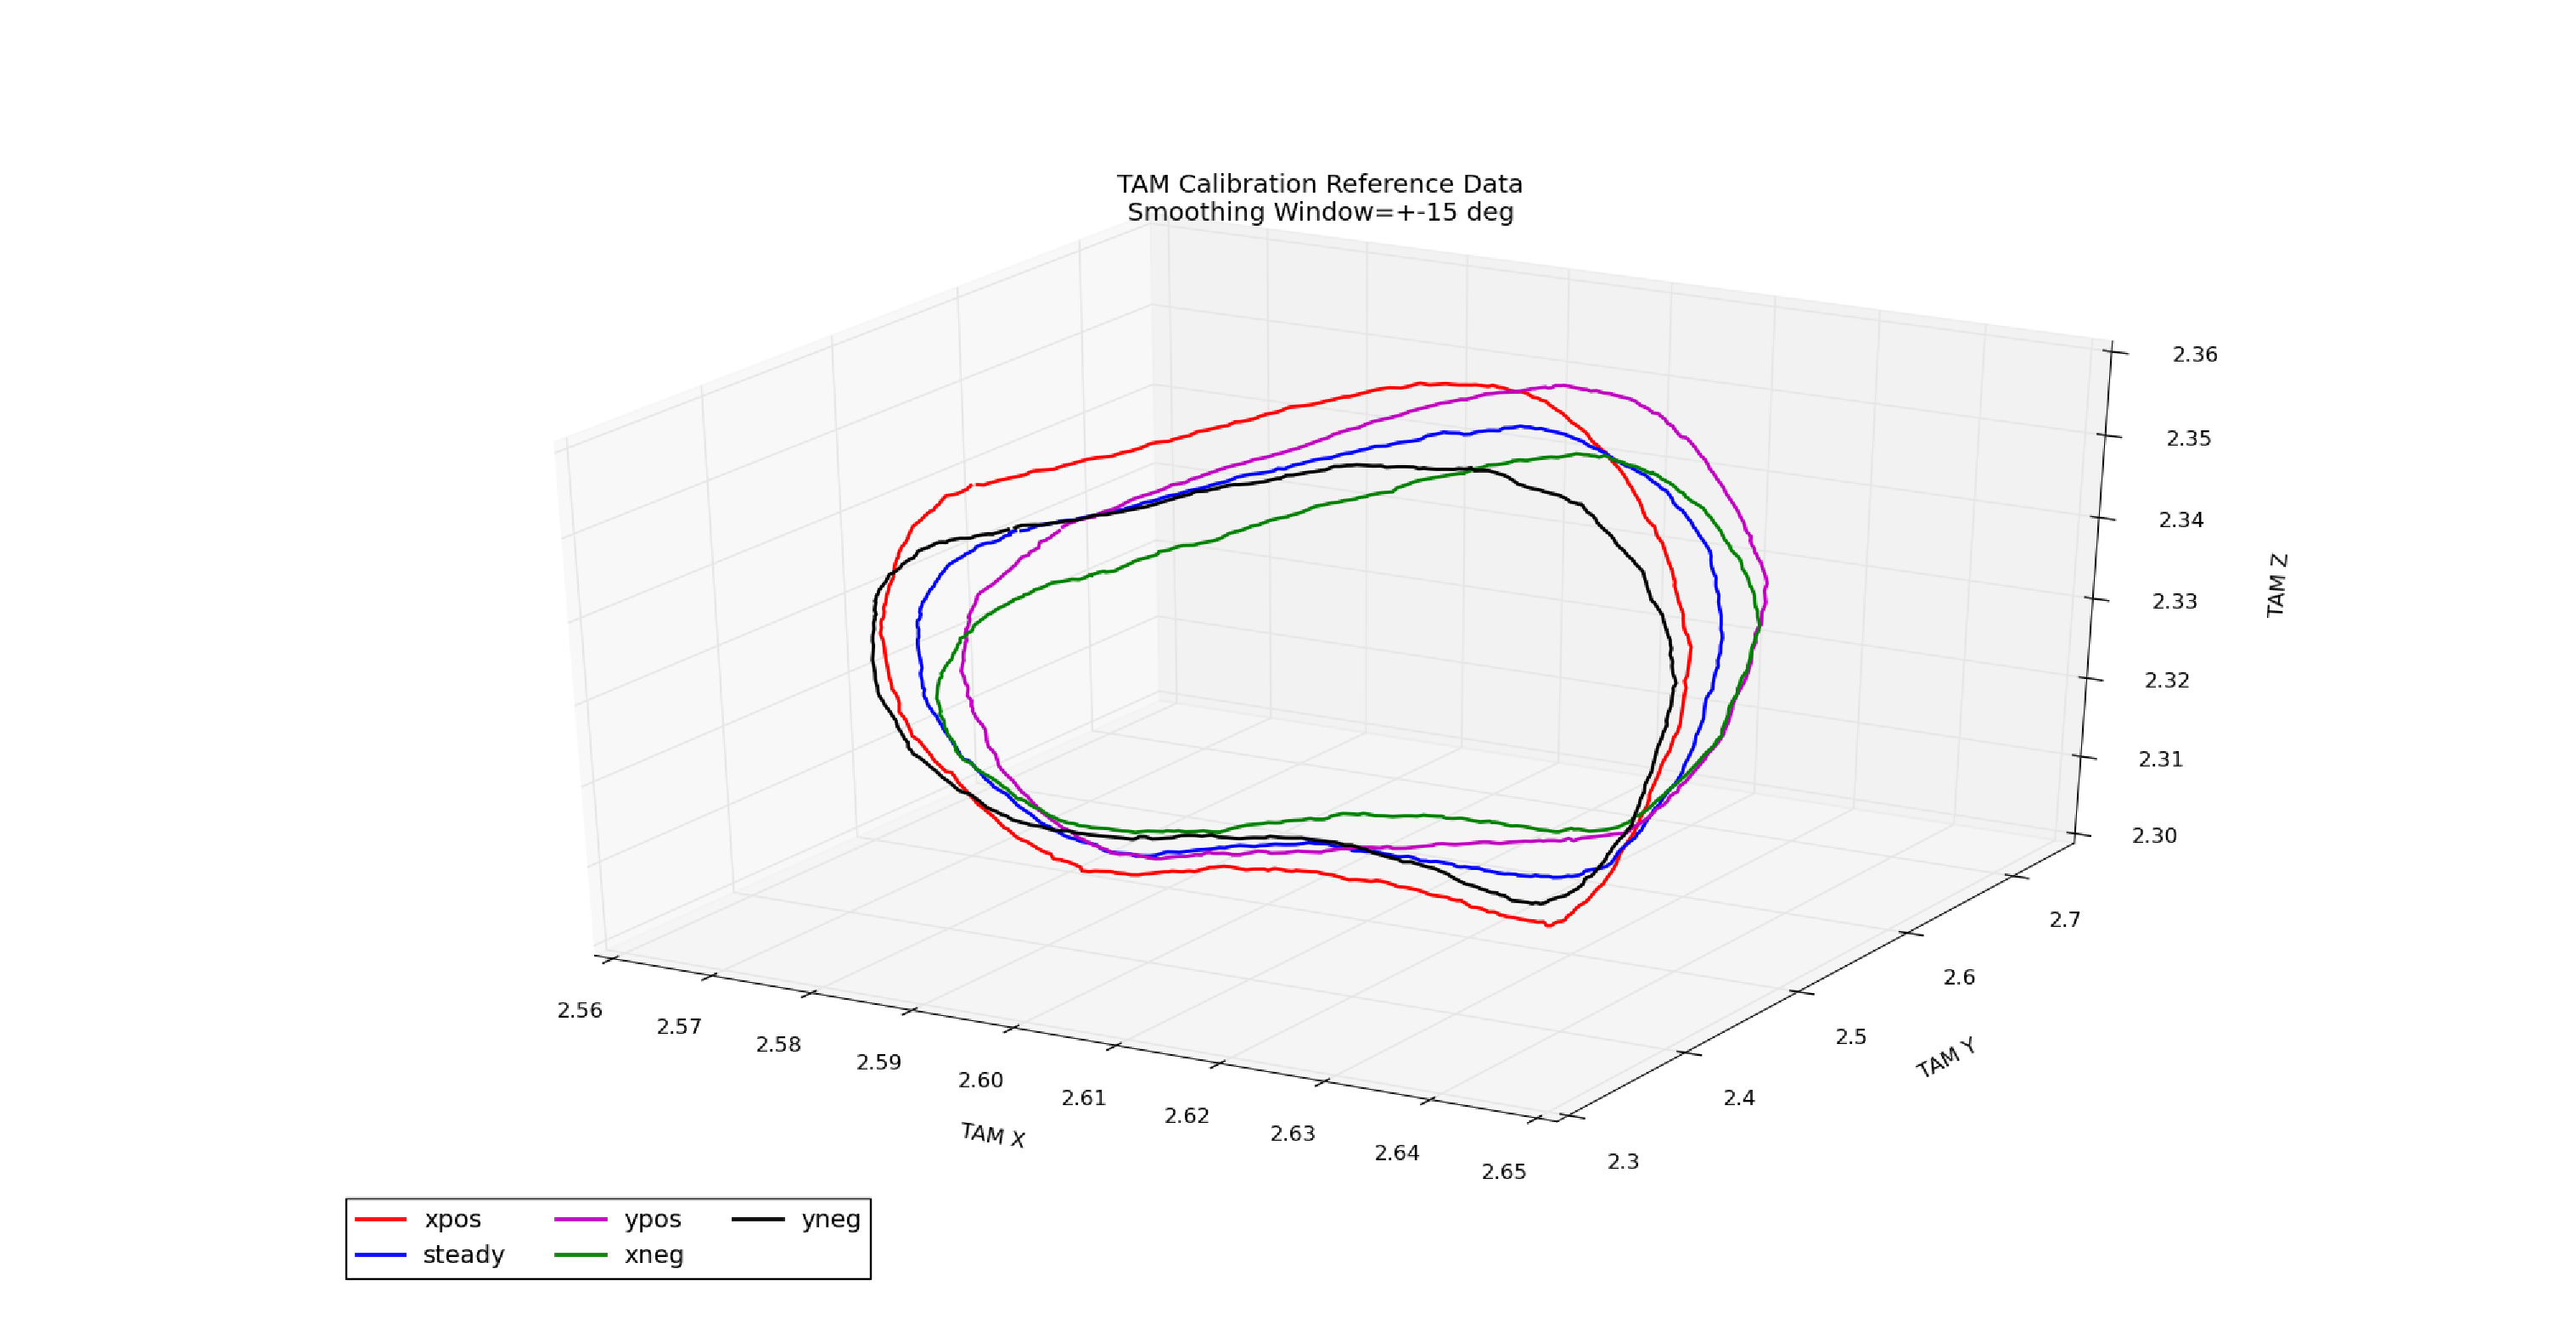
\includegraphics[width=\textwidth]{figures/tam_calibration_ref_15deg_smoothing.eps}
    \caption{$\pm 15^o$ smoothing}
    \label{fig:TAM15degCalibration}
  \end{subfigure}
  \caption{TAM Nutation Reference Values}
  \label{fig:TAMNutationReference}
\end{figure}

The cross shown in Figure \ref{fig:TAMRef191} illustrates the difference in the four nutation reference points compared to the stable point for a 191 degree yaw.  Figure \ref{fig:TAMPoints191} shows the level of noise reduction by the calibration process as the original data points are plotted against the reference nutation voltages.

\begin{figure}[H]
  \centerline{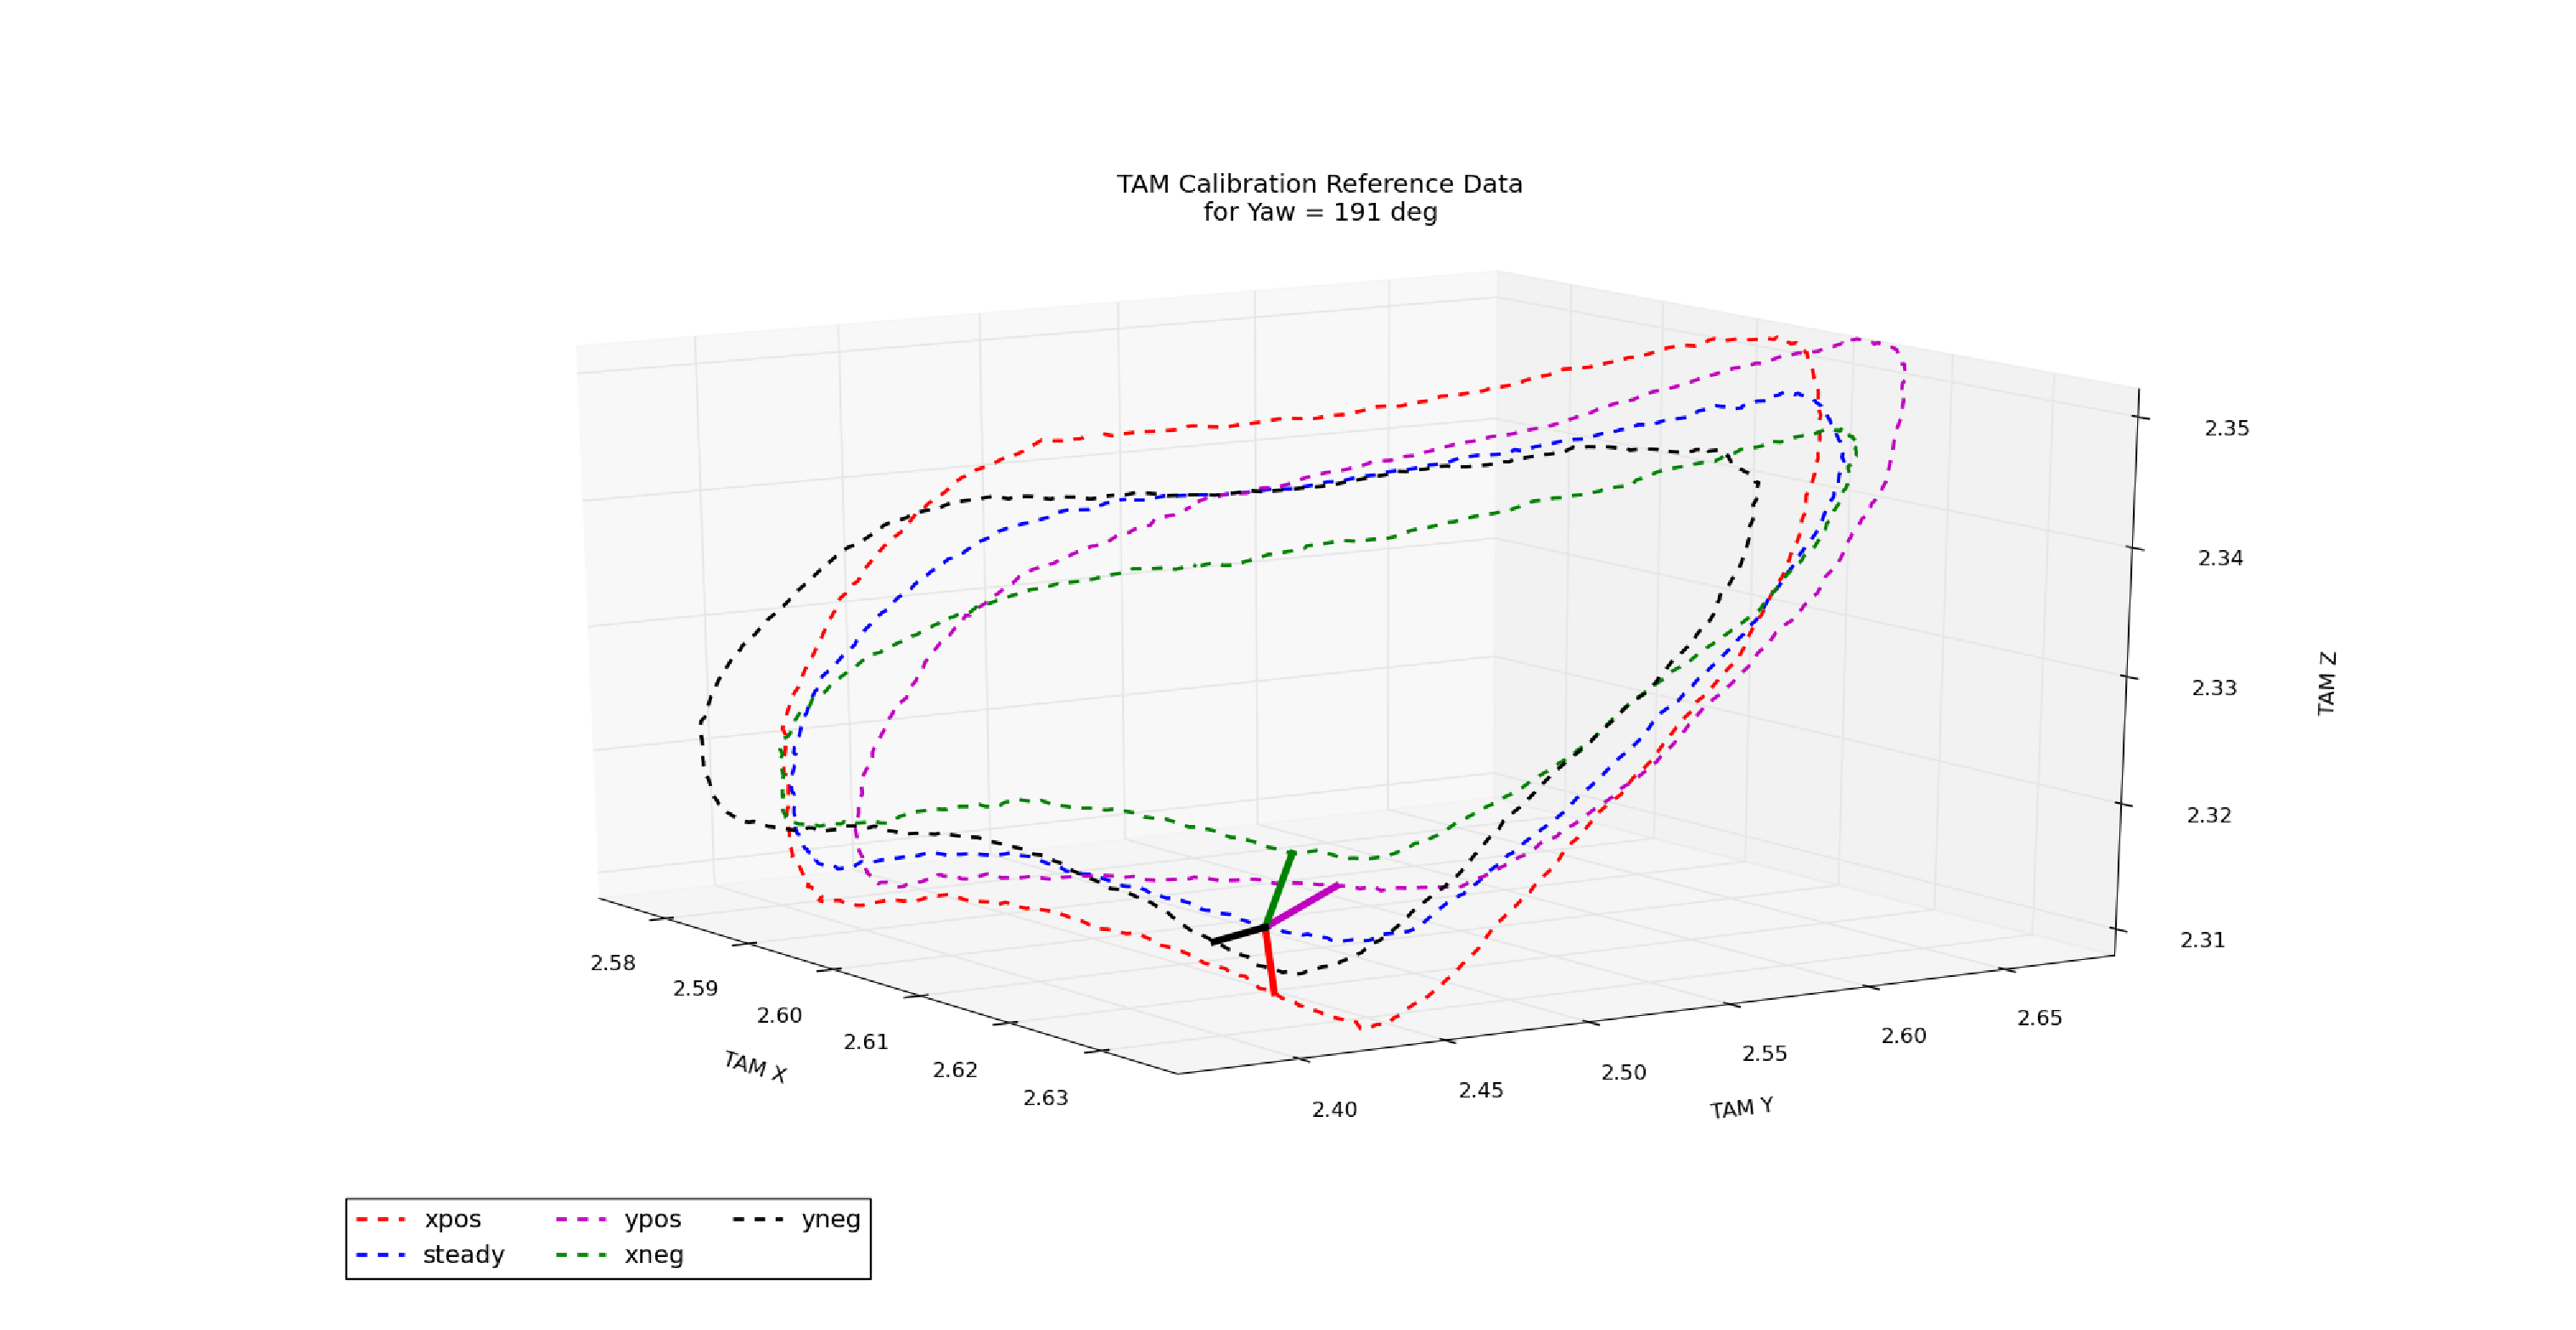
\psfig{file=figures/tam_calibration_ref_for_yaw_191.eps,height=3in}}
  \caption{TAM reference voltages for 191 degree yaw}
  \label{fig:TAMRef191}
\end{figure}

\begin{figure}[H]
  \centerline{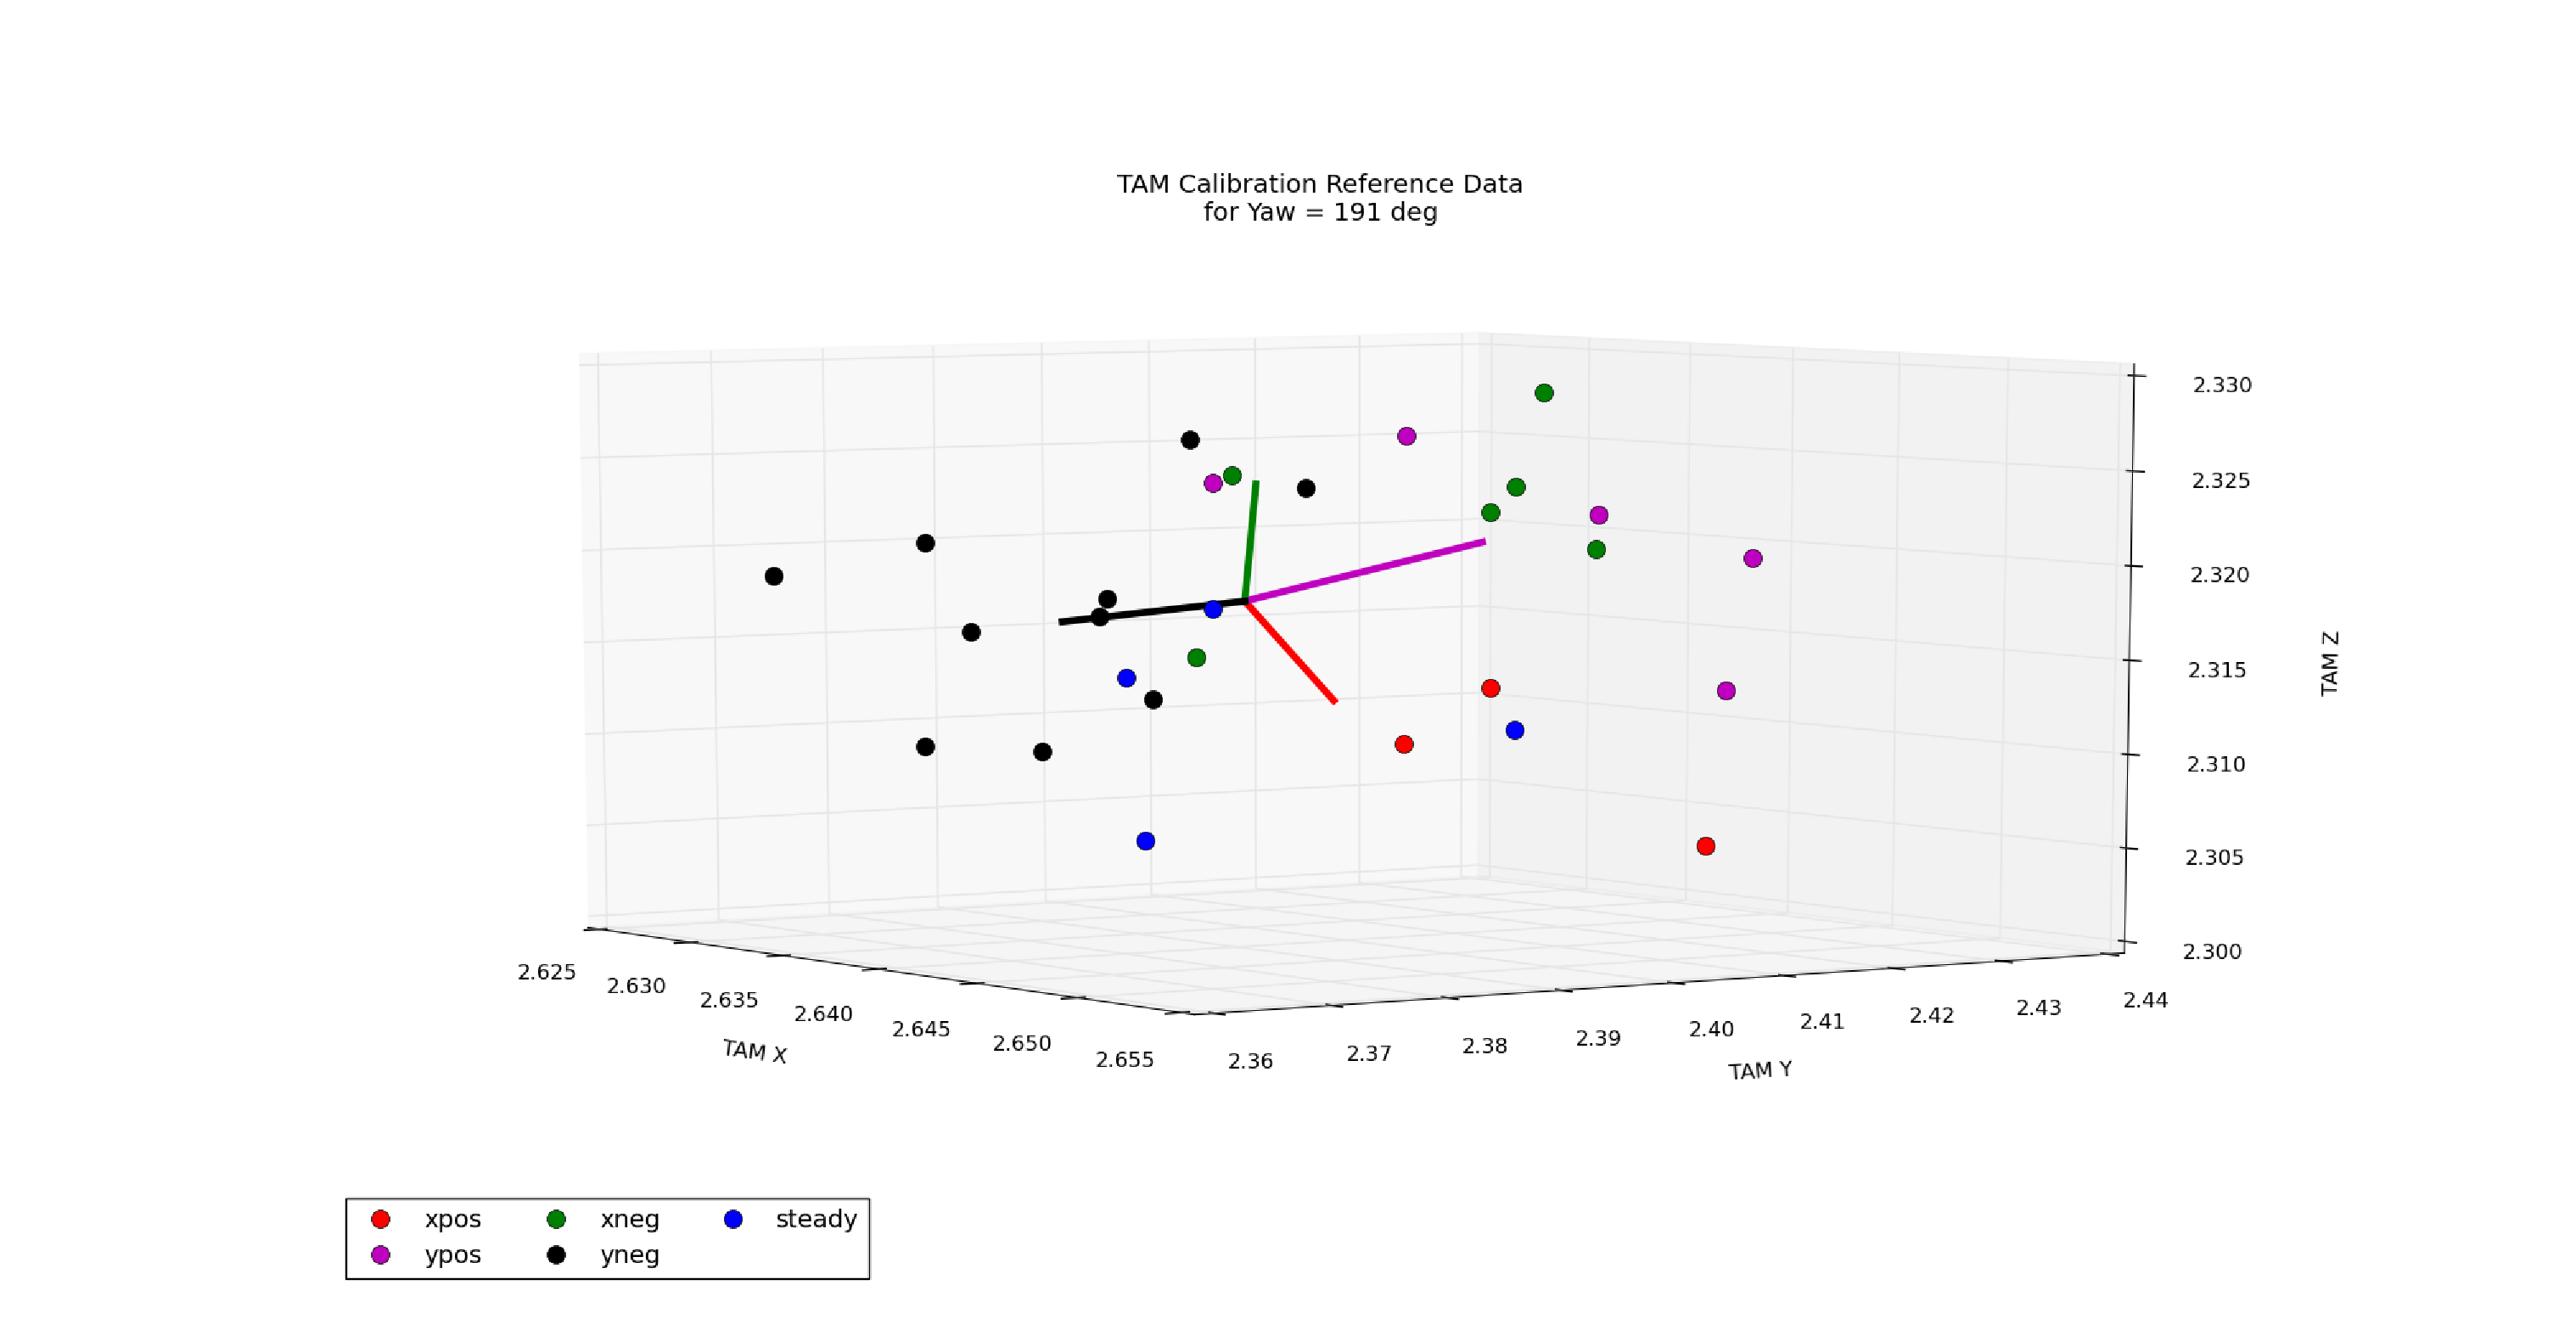
\psfig{file=figures/tam_calibration_191_degree_pts.eps,height=3in}}
  \caption{Closer view of TAM reference voltages for 191 degree yaw}
  \label{fig:TAMPoints191}
\end{figure}

\subsection{Estimating Nutation}

Taking one of the points from $-y$ calibration data to complete the example, Table \ref{tbl:TAMSamplePoints} lists the test point, along with the reference values, obtained from the calibration algorithm above.  The test point plotted in Figure \ref{fig:TAMPoint191} is nearest to the reference $-y$ value, but there is a large gap between the measured value and its associated reference, and other test points as in \ref{fig:TAMPoints191} are far closer to another reference point than its own.

\begin{table}[H]
  \centering
  \begin{tabular}{lc}
    \hline
    Test Point       & $(2.63, 2.37, 2.32)$ \\ \hline
    Steady Reference & $(2.63, 2.40, 2.32)$ \\ \hline
    xpos Reference   & $(2.63, 2.42, 2.31)$ \\ \hline
    ypos Reference   & $(2.64, 2.42, 2.32)$ \\ \hline
    xneg Reference   & $(2.64, 2.39, 2.32)$ \\ \hline
    yneg Reference   & $(2.63, 2.39, 2.32)$ \\ \hline
  \end{tabular}
  \caption{TAM sample reference points}
  \label{tbl:TAMSamplePoints}
\end{table}


\begin{figure}[H]
  \centerline{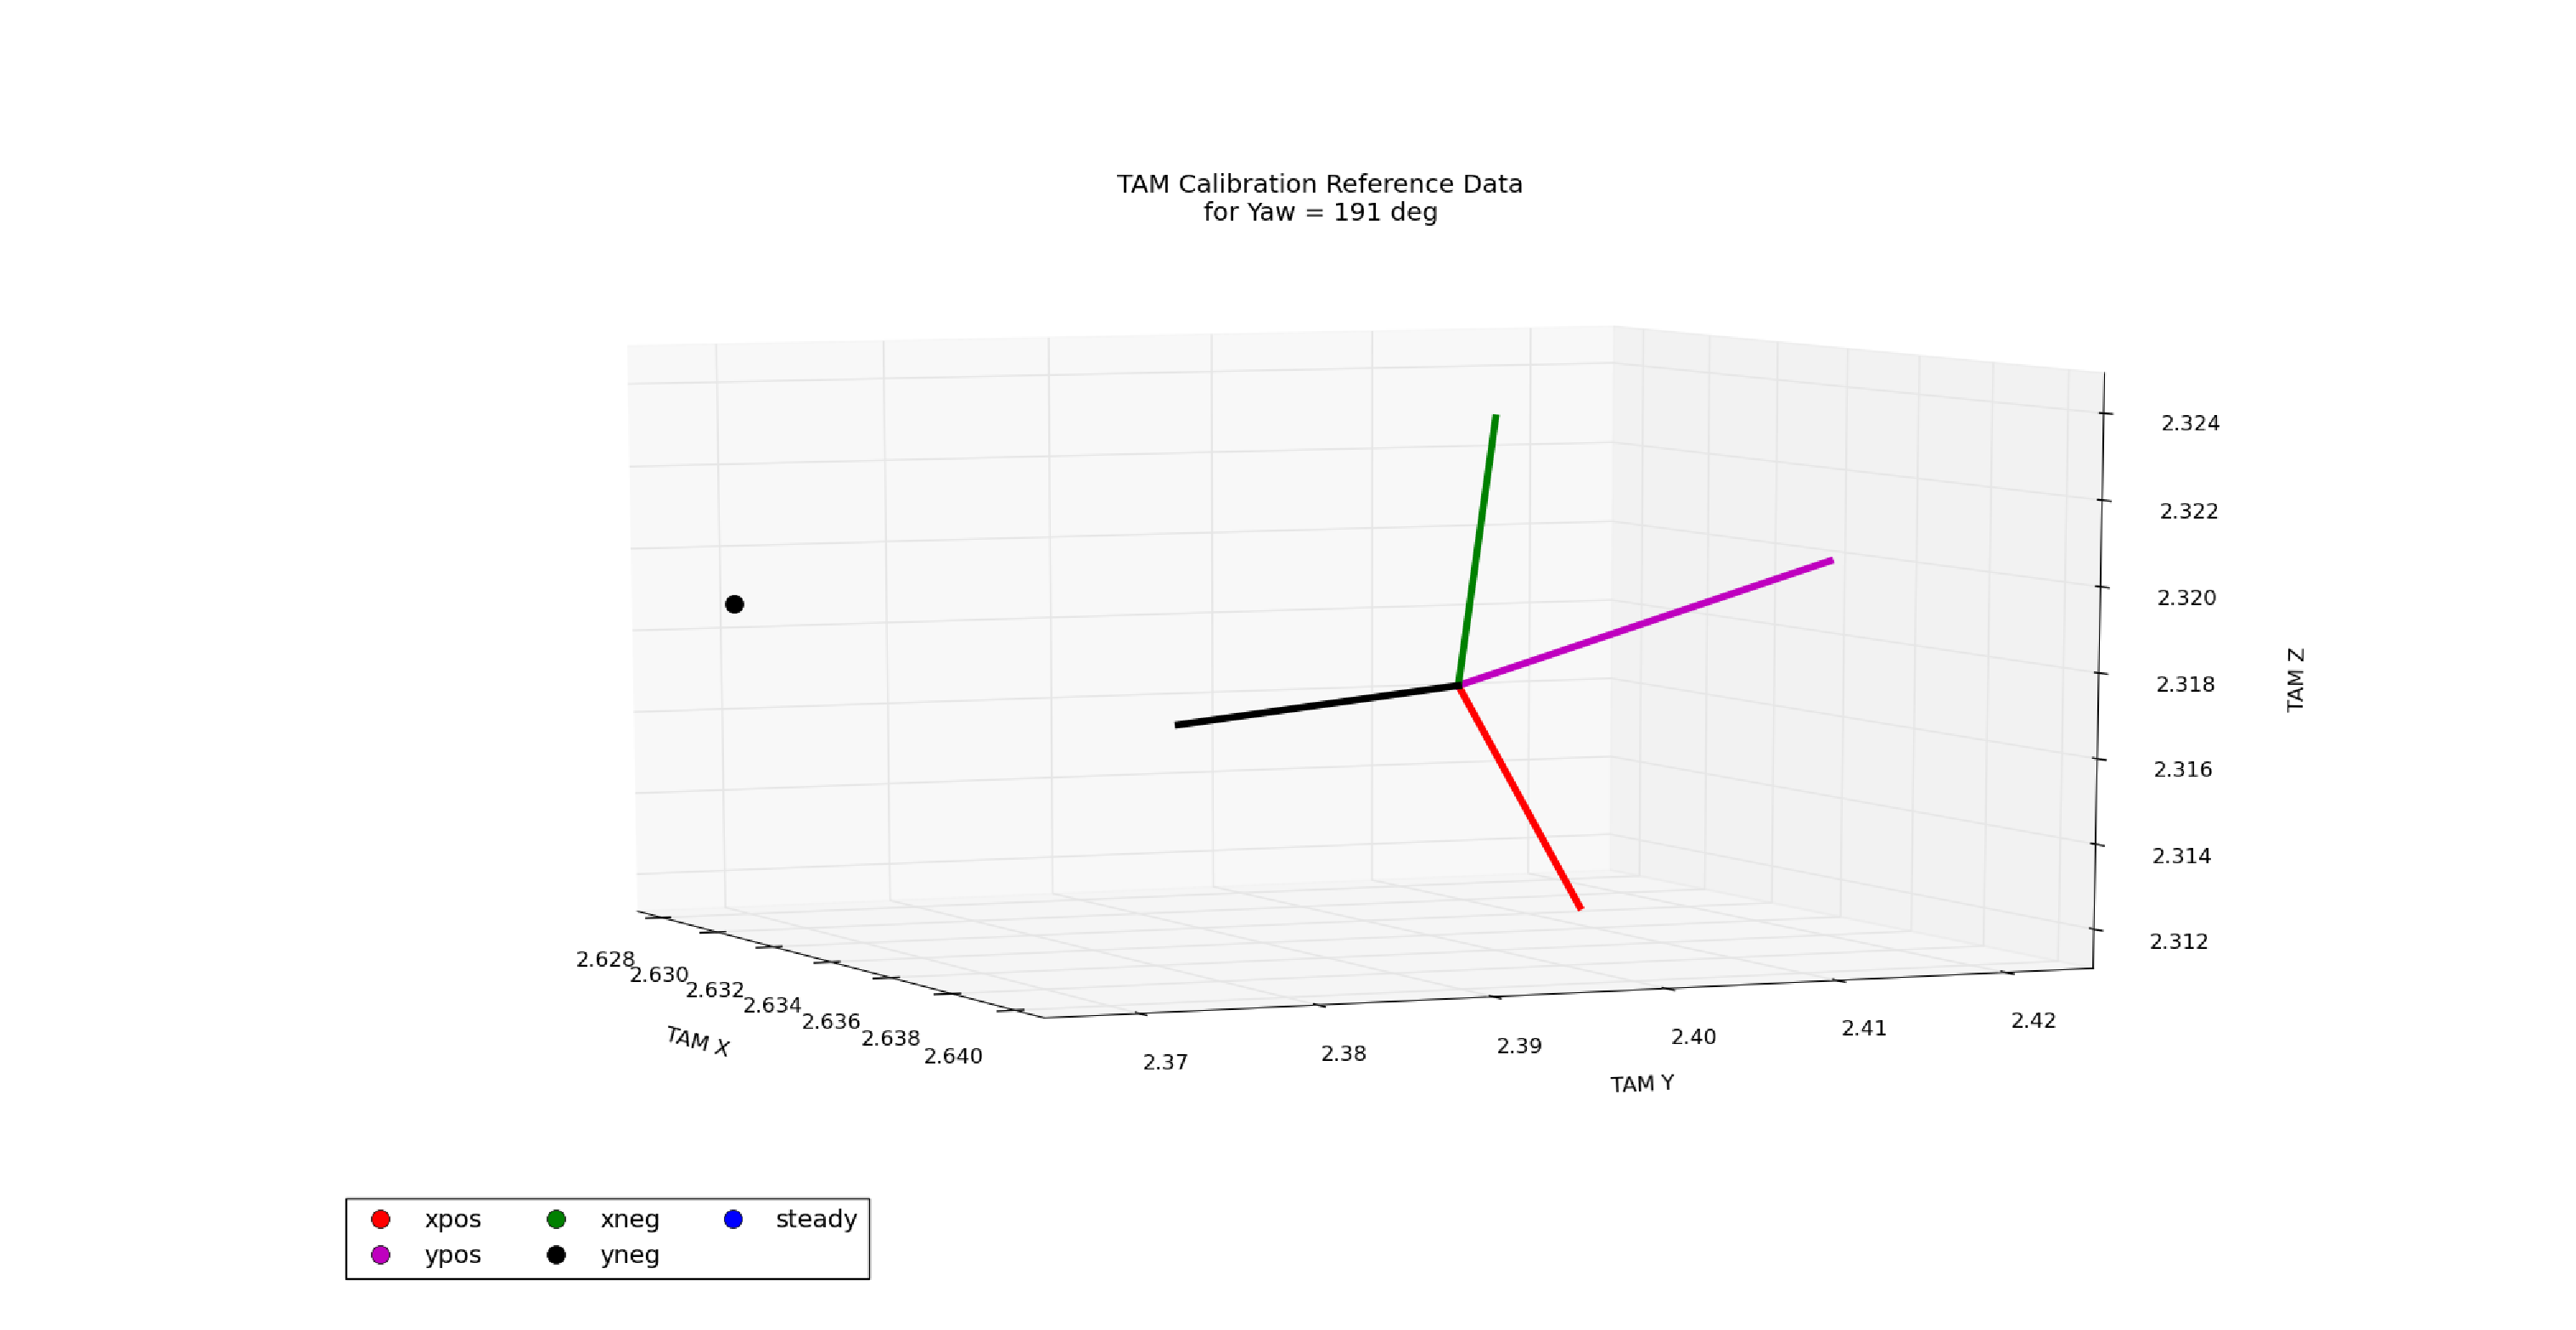
\psfig{file=figures/tam_calibration_191_degree_pt.eps,height=3in}}
  \caption{TAM sample data point for nutation calculation}
  \label{fig:TAMPoint191}
\end{figure}

In order to determine the best approximation for the measured nutations, a number of combinations of approaches are attempted including using the proportion between two estimates, normalizing the reference vectors, projecting the point to the plane consisting of the two nearest vectors, and creating a conversion of the x and y vectors to an orthogonal space.  Some cases provided slightly lower classification error rates when compared to the original calibration test set, but any improvements are not significant.  For simplicity and speed, the measurement estimate for nutation is reduced to a ``nearest neighbor'' classification \cite{nearestneighbor} where the closest reference point is chosen as the best approximation.

Despite the improved speed and simplicity, this classification method has some large faults, the biggest of which is the resulting chattered signal that is relayed to the estimator state.  This is because there are no continuum of values, the nutation state jumps between the five calibration states of level, and each of the $14^o$ nutations.  Further work is needed to refine this technique.


\chapter{HIGH INTEGRITY STATE ERROR AND ADJUSTMENTS}
\label{chap:StateError}

A process for quantifying the error between two states is fundamental in any estimation or control technique.  The state estimate error $\bs{\hat{x}}_e$ compares the measured state $\bs{x}$ to the estimated state $\bs{\hat{x}}$.  The state control error $\bs{x}_e$ represents the offset between the estimated state $\bs{\hat{x}}$ and the desired system state $\bs{x}_d$.  In other words, the state errors can be represented as
\begin{subequations}
  \begin{align}
    \bs{\hat{x}}_e &= \bs{\hat{x}} - \bs{x} \\
    \bs{x}_e &= \bs{\hat{x}} - \bs{x}_d
  \end{align}
  \label{eqn:StateError}
\end{subequations}

Proceeding through the observer-based controller, $\bs{x}$ represents the measured state, $\bs{\hat{x}}_e$ represents the error between the estimated state and the measured, $\bs{\hat{x}}$ is the estimated state, $\bs{x}_e$ is the error between the estimated and desired state, and finally $\bs{x}_d$ is the desired state.
\begin{equation}
  \bs{x} \to \bs{\hat{x}}_e \to \bs{\hat{x}} \to \bs{x}_e \to \bs{x}_d
\end{equation}

Sections \ref{sec:StateDifference} through \ref{subsec:ThetaMultiplierWithQuaternionVectorBalancing} outline the series of improvement made to the accuracy of the state error representation.  For comparison and to demonstrate their use with TSatPy, these sections will base their comparison on a single update to a proportional estimator.

\begin{equation}
  \bs{\hat{x}(t_{k+1})} = \bs{\hat{x}}(t_{k}) + \bs{K_p} ( \bs{\hat{x}}(t_{k}) - \bs{x}(t_{k}) )
  \label{eqn:PEstimatorStateDiff}
\end{equation}

The sample error calculation based on Equation (\ref{eqn:PEstimatorStateDiff}) where the last estimated state, $\bs{\hat{x}}(t_{k})$, is a $190^o$ rotation about $+z$-axis, and an angular velocity of $\omega_z = 3$ rad/sec.  The associated state, $\bs{x}(t_{k})$, is a $44^o$ rotation about the axis $0 \bs{i} + 0.1 \bs{j} + 1\bs{k}$ and a angular velocity of $\omega_z = 3.1$ rad/sec.  That is,
\begin{subequations}
  \begin{align}
    \bs{\hat{x}}(t_{k})
    = \begin{bmatrix}  \bs{\hat{q}}(t_{k}) \\ \bs{\hat{\omega}}(t_{k}) \end{bmatrix}
    &= \begin{bmatrix} 0 \bs{i} +0 \bs{j} -0.996195 \bs{k} -0.0871557 \\ 0 \bs{i} +0 \bs{j} +3 \bs{k} \end{bmatrix}\\
    \bs{x}(t_{k})
    = \begin{bmatrix}  \bs{q}(t_{k}) \\ \bs{\omega}(t_{k}) \end{bmatrix}
    &= \begin{bmatrix} 0 \bs{i} -0.0372747 \bs{j} -0.372747 \bs{k} +0.927184 \\ 0 \bs{i} +0 \bs{j} +3.1 \bs{k} \end{bmatrix}
  \end{align}
  \label{eqn:StateDifferenceQuaternionSamples}
\end{subequations}

Snippet \ref{code:estimated_and_measured_states} shows how the estimated and measured states from Equation (\ref{eqn:StateDifferenceQuaternionSamples}) are created using this thesis' TSatPy attitude dynamics and controls software.
\begin{listing}[H]
\begin{singlespace}
  \begin{minted}[mathescape,linenos,numbersep=10pt,frame=lines,framesep=2mm]{python}
from TSatPy.State import Quaternion, QuaternionError, State, BodyRate
import numpy as np

x_hat = State(
    Quaternion([0,0,1],radians=190/180.0*np.pi),
    BodyRate([0,0,3]))
x_m = State(
    Quaternion([0,0.1,1],radians=44/180.0*np.pi),
    BodyRate([0,0,3.1]))
print("x_hat:  %s" % (x_hat))
print("x_m:    %s" % (x_m))

# Prints Out
# x_hat:  <Quaternion [-0 -0 -0.996195], -0.0871557>,
#         <BodyRate [0 0 3]>
# x_m:    <Quaternion [-0 -0.0372747 -0.372747], 0.927184>,
#         <BodyRate [0 0 3.1]>
  \end{minted}
\caption{Create estimated $\bs{\hat{x}}$ and measured $\bs{x}$ states}
\label{code:estimated_and_measured_states}
\nocite{minted}
\end{singlespace}
\end{listing}

Section \ref{sec:StateDifference} inspects a singe update to a quaternion based P-estimator.  The procedure follows the common process of taking the difference in values to establish an error and correcting the estimate by a fraction of the error.  This method is well established and accepted for many system's state representation, but applying the same procedure to a quaternion based attitude creates a lot of error.

Section \ref{sec:QuaternionMultiplicativeError} introduces the quaternion multiplicative error as a method for combining quaternions while preserving rotational representation.

Section \ref{sec:QuaternionMultiplicativeCorrection} tests methods for scaling quaternion errors such that they maintain the unit norm and that scaling the error measurement by a gain has a clear connection to the physical separation of two attitudes.

\section{State Difference}
\label{sec:StateDifference}

The traditional method for calculating state estimation and control errors is to calculate an element-wise difference.  TableSat has a seven element state in matrix form and expanding Equation (\ref{eqn:StateError}) becomes
\begin{equation}
  \begin{aligned}
    \bs{\hat{x}}_e(t_{k}) &= \begin{bmatrix}  \bs{\hat{q}}_e(t_{k}) \\ \bs{\hat{\omega}}_e(t_{k}) \\ \end{bmatrix} \\
    &= \begin{bmatrix} (\hat{q}_1 - q_{1}) \bs{i} + (\hat{q}_2 - q_{2}) \bs{j} + (\hat{q}_3 - q_{3}) \bs{k} + \hat{q}_0 - q_{0} \\ (\hat{\omega}_x - \omega_{x}) \bs{i} + (\hat{\omega}_y - \omega_{y}) \bs{j} + (\hat{\omega}_z - \omega_{z}) \bs{k} \end{bmatrix}
  \end{aligned}
  \label{eqn:StateDifference}
\end{equation}
Calculating the difference between the example estimated and measured states in Equation (\ref{eqn:StateDifferenceQuaternionSamples}) yields a state difference of
\begin{equation}
  \begin{aligned}
    \bs{\hat{x}}_e(t_{k})
    = \begin{bmatrix}  \bs{\hat{q}}_e(t_{k}) \\ \bs{\hat{\omega}}_e(t_{k}) \end{bmatrix}
    &= \begin{bmatrix} 0 \bs{i} +0.0372747 \bs{j} -0.623447 \bs{k} -1.01434 \\ 0 \bs{i} +0 \bs{j} -0.1 \bs{k} \end{bmatrix}
  \end{aligned}
  \label{eqn:StateDifferenceSample}
\end{equation}
The same difference is calculated with TSatPy as
\begin{listing}[H]
\begin{singlespace}
  \begin{minted}[mathescape,linenos,numbersep=10pt,frame=lines,framesep=2mm]{python}
x_e = State(
    Quaternion(x_hat.q.vector - x_m.q.vector,
        x_hat.q.scalar - x_m.q.scalar),
    x_hat.w - x_m.w)
print("x_e:  %s" % (x_e))

# Prints Out
# x_e:  <Quaternion [0 0.0372747 -0.623447], -1.01434>,
#       <BodyRate [0 0 -0.1]>
  \end{minted}
\caption{State difference creates an invalid rotational quaternion}
\label{code:state_difference}
\nocite{minted}
\end{singlespace}
\end{listing}

The body rate error calculations of $\omega_ze = -0.1$ is directly related to the 0.1 rad/sec difference in angular velocities between the measured and estimated states.  The difference in quaternion parameters of $\bs{q}_e = 0 \bs{i} +0.0372747 \bs{j} -0.623447 \bs{k} -1.01434$ however poses no connection to the physical difference in states as the scalar quantity in the error quaternion is outside the possible range for any rotational quaternion, so using this difference to adjust the quaternion estimate will only add a source of error.

Although the difference in quaternions is shown to not have any connection to the physical difference in attitudes, the difference in states is still regularly used in quaternion estimation implementations.  If the example from Equation (\ref{eqn:StateDifferenceSample}) is carried into a proportional estimator with a gain value of $K_{qp} = -0.8$, the quaternion adjustment, $\bs{q}_{adj}$, and predicted next attitude, $\bs{\hat{q}}(t_{k+1})$, are
\begin{equation}
  \begin{aligned}
    \bs{q}_{adj} = -0.8 \cdot \bs{q}_e =& -0.8 \cdot (0 \bs{i} + 0.0372747 \bs{j} -0.623447 \bs{k} -1.01434 ) \\
                       =& 0 \bs{i} -0.0298198 \bs{j} +0.498758 \bs{k} +0.811472 \\
    \bs{\hat{q}(t_{k+1})} =& \bs{\hat{q}(t_{k})} + \bs{q}_{adj} \\
                       =& 0 \bs{i} -0.0298198 \bs{j} -0.497437 \bs{k} + 0.724316 \\
  \end{aligned}
  \label{eqn:quat_add_adj}
\end{equation}
Equation (\ref{eqn:quat_add_adj}) is completed with TSatPy software by
\begin{listing}
\begin{singlespace}
  \begin{minted}[mathescape,linenos,numbersep=10pt,frame=lines,framesep=2mm]{python}
K_pq = -0.8
q_hat = x_hat.q
q_e = x_e.q
q_adj = Quaternion(K_pq * q_e.vector, K_pq * q_e.scalar)
q_hat_new = Quaternion(q_hat.vector + q_adj.vector,
        q_hat.scalar + q_adj.scalar)

print("q_e:         %s" % (q_e))
print("q_adj:       %s" % (q_adj))
print("q_hat_new:   %s" % (q_hat_new))
print("|q_hat_new|: %g" % (q_hat_new.mag))

# Prints Out
# q_e:         <Quaternion [0 0.0372747 -0.623447], -1.01434>
# q_adj:       <Quaternion [-0 -0.0298198 0.498758], 0.811472>
# q_hat_new:   <Quaternion [-0 -0.0298198 -0.497437], 0.724316>
# |q_hat_new|: 0.879185
  \end{minted}
\caption{Quaternion additive correction causes pts to converge to origin}
\label{code:additive_correction}
\nocite{minted}
\end{singlespace}
\end{listing}

After $\bs{q}_{adj}$ is added to the original estimate $\bs{\hat{q}}$ with the purpose of improving the estimated state, the predicted attitude quaternion changes from the correct unit norm to $ \| \bs{\hat{q}(t_{k+1})} \| = 0.879185$ after the update.  Since failing to conform to the unit magnitude for rotational quaternions, this newly estimated attitude quaternion corrupts the systems state especially over multiple steps and long simulations.  For rotational quaternions with norms less that the unit quaternion, the rotated points eventually converge to the origin.  If the adjustment results in a rotational quaternion larger than a unit magnitude, the rotated points diverge from the origin.

Snippet \ref{code:bad_rotational_quaternion} validates that rotating point $A (1,0,0)$ with the malformed predicted state from Snippet \ref{code:additive_correction} results in the point collapsing toward the origin.
\begin{listing}
\begin{singlespace}
  \begin{minted}[mathescape,linenos,numbersep=10pt,frame=lines,framesep=2mm]{python}
A = np.mat([[1,0,0]])
A = q_hat_new.rotate_points(A)
print("A * A.T:   %s" % (A * A.T))

# Prints Out
# A * A.T:   [[ 0.5974769]]
  \end{minted}
\caption{Rotate a point with a bad rotational quaternion}
\label{code:bad_rotational_quaternion}
\nocite{minted}
\end{singlespace}
\end{listing}

To take into account the dilation or compression of points, the adjusted quaternion is commonly scaled back to a unit quaternion through a standard vector normalization:
\begin{equation}
  \bs{\hat{q}}_n = \frac{\bs{q}_v + q_0}{\sqrt{\bs{q}_v \bullet \bs{q}_v + q_0^2}}
  \label{eqn:NormalizeQuaternion}
\end{equation}
Continuing from Snippet \ref{code:additive_correction}, the predicted quaternion $\bs{\hat{q}}(t_{k+1})$ is normalized then inspected to determine what rotation it represents.
\begin{listing}
\begin{singlespace}
  \begin{minted}[mathescape,linenos,numbersep=10pt,frame=lines,framesep=2mm]{python}
print("q_hat_new:   %s" % (q_hat_new))
q_hat_new.normalize()
print("q_hat_new:   %s" % (q_hat_new))
print("|q_hat_new|: %g" % (q_hat_new.mag))

# Prints Out
# q_hat_new:   <Quaternion [-0 -0.0298198 -0.497437], 0.724316>
# q_hat_new:   <Quaternion [-0 -0.0339175 -0.565793], 0.823849>
# |q_hat_new|: 1

e, r = q_hat_new.to_rotation()
print("e: <%g, %g, %g>\ndegree: %g" % (
    e[0,0],e[1,0],e[2,0], r * 180.0 / np.pi))

# Prints Out
# e: <-0, -0.0598395, -0.998208>
# degree: 69.056
  \end{minted}
\caption{Normalizing the quaternion only makes state error worse}
\label{code:normalized_no_work}
\nocite{minted}
\end{singlespace}
\end{listing}

The newly estimated state is equivalent to a $69$ degree rotation about the Euler axis
\begin{equation}
  \hat{\bs{e}} = \begin{bmatrix} 0 & -0.0598395 & -0.998208 \end{bmatrix}^T
\end{equation}
While this state estimate conforms to the unit quaternion requirement and will no longer corrupt rotations, it has little in common with the desired $0.8$ proportional gain used the estimator's design.



\section{Quaternion Multiplicative Error}
\label{sec:QuaternionMultiplicativeError}

The previous sections have established that the state difference approach for adjusting for errors in attitude measurements has significant issues especially for low frequency updates with high error values.  Quaternion multiplication defined in Equation (\ref{eqn:QuaternionMultiplication}) is used to calculate quaternion multiplication and can be used to modify the attitude while not introducing corruption into the model if used with rotational unit quaternions.

If the estimated and measured states converge using multiplicative correction, the error quaternion converges to the identity quaternion.  The identity quaternion, as with the identity matrix, is the quantity that when multiplied by another quaternion, does not modify its value.  This identity holds true for general as well as rotational quaternions.

\begin{equation}
  \bs{q}_I = 0 \bs{i} + 0 \bs{j} + 0 \bs{k} + 1
\end{equation}

An Identity function is created it the TSatPy.State module to construct an identity quaternion.

\begin{listing}
\begin{singlespace}
  \begin{minted}[mathescape,linenos,numbersep=10pt,frame=lines,framesep=2mm]{python}
from TSatPy import State

q = State.Quaternion([1,2,3], 4)
print("q       = %s" % q)
q_I = State.Identity()
print("q_I     = %s" % q_I)
print("q_I * q = %s" % (q_I * q))

# Prints Out
# q       = <Quaternion [1 2 3], 4>
# q_I     = <Quaternion [0 0 0], 1>
# q_I * q = <Quaternion [1 2 3], 4>
  \end{minted}
\caption{Working with a quaternion identity}
\nocite{minted}
\end{singlespace}
\end{listing}

Rotational quaternions are considered equal if they represent the same attitude.  The same attitude can be represented by more than one distinct quaternion, so a strict equality is not adequate.  The test for equality is accomplished by using the quaternion conjugate $\bs{q}^*$ such that

\begin{subequations}
  \begin{align}
    \bs{\hat{q}} = \bs{q} & \iff \bs{\hat{q}}^* \otimes \bs{q} = \bs{q}^* \otimes \bs{\hat{q}} = \bs{q}_I \text{ or } -\bs{q}_I \\
    \text{where } \bs{q}^* &= \begin{bmatrix} -\bs{v} \\ q_0 \end{bmatrix}
  \end{align}
  \label{eqn:QuaternionEquality}
\end{subequations}

Snippet \ref{code:quaternion_conj} shows how two distinct quaternions can represent the same attitude and that the test for equality in Equation (\ref{eqn:QuaternionEquality}) holds true.

\begin{listing}
\begin{singlespace}
  \begin{minted}[mathescape,linenos,numbersep=10pt,frame=lines,framesep=2mm]{python}
a = Quaternion([0,0,1],radians=190/180.0*np.pi)
b = Quaternion([0,0,1],radians=(190 + 360)/180.0*np.pi)

print("a:          %s" % (a))
print("b:          %s" % (b))
print("a.conj * b: %s" % (a.conj * b))

# Prints Out
# a:          <Quaternion [-0 -0 -0.996195], -0.0871557>
# b:          <Quaternion [0 0 0.996195], 0.0871557>
# a.conj * b: <Quaternion [0 0 -3.46945e-16], -1>
  \end{minted}
\caption{Quaternion equality testing using the quaternion conjugate}
\label{code:quaternion_conj}
\nocite{minted}
\end{singlespace}
\end{listing}

Equation (\ref{eqn:QuaternionEquality}) provides a method for determining whether two quaternions represent the same attitude, it can also be used to quantify the difference between two rotational quaternions using the multiplicative comparison
\begin{equation}
  \bs{q}_e = \bs{q}^* \otimes \bs{\hat{q}}
  \label{eqn:QuaternionError}
\end{equation}

Continuing with the some example, given the measured and estimated states from Equation (\ref{eqn:StateDifferenceQuaternionSamples}), the multiplicative quaternion error between these states evaluates to

\begin{equation}
  \begin{aligned}
    \bs{q}_e = & \bs{q}^* \otimes \bs{\hat{q}} \\
    = & \big( 0 \bs{i} +0.0372747 \bs{j} +0.372747 \bs{k} +0.927184 \big) \\
    & \otimes \big( 0 \bs{i} +0 \bs{j} -0.996195 \bs{k} -0.0871557 \big)\\
    = & -0.0371329 \bs{i} -0.00324871 \bs{j} -0.956143 \bs{k} +0.29052
  \end{aligned}
  \label{eqn:QuaternionErrorSample}
\end{equation}
The sample error measurement in Equation (\ref{eqn:QuaternionErrorSample}) relates well to the deviations in the estimated and measured attitudes, as it represents a 146 degree rotation about the Euler axis $-0.0388067 \bs{i} -0.00339514 \bs{j} -0.999241\bs{k}$ which rotates the estimated quaternion to match up identically to the measured state.  The multiplicative error correction quaternion also solves the issue encountered previously where the magnitude of the error quaternion does not remain fixed at the unit quaternion.

\begin{listing}
\begin{singlespace}
  \begin{minted}[mathescape,linenos,numbersep=10pt,frame=lines,framesep=2mm]{python}
from TSatPy.State import QuaternionError
q_e = QuaternionError(x_hat.q, x_m.q)

print("q_e:   %s" % (q_e))
print("|q_e|: %s" % (q_e.mag))
e, r = q_e.to_rotation()
print("e:     <%g, %g, %g>\ndegree: %g" % (
    e[0,0],e[1,0],e[2,0], r * 180.0 / np.pi))

# Prints Out
# q_e:   <Quaternion [-0.0371329 -0.00324871 -0.956143], 0.29052>
# |q_e|: 1.0
# e:     <-0.0388067, -0.00339514, -0.999241>
# degree: 146.222
  \end{minted}
\caption{Converting a rotational quaternion back into it's rotational form}
\label{code:quat_to_rot}
\nocite{minted}
\end{singlespace}
\end{listing}

\section{Quaternion Multiplicative Correction}
\label{sec:QuaternionMultiplicativeCorrection}

Section \ref{sec:QuaternionMultiplicativeError} establishes a method for quantifying differences in attitude and that preserves the integrity of the rotational quaternion while creating a representative measure of the state error.  A series of options are investigated to determine how to incorporate gain parameters into the error measurements for use with estimation and control techniques.

\subsection{Parameter Multiplier}
\label{subsec:ParameterMultiplier}

With a parameter multiplier method, the four parameters of the error quaternion are scaled by a term $\bs{K_p}$, similar to the standard proportional adjustment:

\begin{equation}
  \bs{q}_{adj} = \bs{K_p} \bs{q}_e
    = \bs{K_p} \begin{bmatrix} \bs{v}_e \\ q_{e0} \end{bmatrix}
    = \begin{bmatrix} \bs{K_{vp}}\bs{v}_e \\ K_{0p} \cdot q_{e0} \end{bmatrix}
  \label{eqn:ParameterMultiplier}
\end{equation}
where the $\bs{K_{vp}}$ term is a 3x3 matrix.  Since $\bs{v}_e$ defines the axis of rotation for the quaternion which can change in magnitude but not direction $\bs{K_{vp}}\bs{v}_e$ is simplified to
\begin{equation}
  \bs{K_{vp}} \bs{v}_e = \lambda \bs{v}_e
  \label{eqn:QuaternionVectorCorrection}
\end{equation}
where $\lambda$ is a scalar.
Combining \ref{eqn:QuaternionVectorCorrection} with \ref{eqn:ParameterMultiplier} yields
\begin{equation}
  \bs{q}_{adj} = \begin{bmatrix} \lambda \bs{v}_e \\ K_{0p} \cdot q_{e0} \end{bmatrix}
  \label{eqn:QuaternionScalarMultiplier}
\end{equation}
thus, Reducing the tunable parameters for the proportional quaternion estimator to $\lambda$ and $K_{0p}$.  This configuration, shares the same flaws as the state difference approach described previously where the magnitude of the adjusted quaternion can vary from the unit quaternion causing dilation or compression of rotated points.  Continuing from Snippet \ref{code:quat_to_rot} the $\bs{q}_e$ is a unit norm quaternion representing the error between two attitudes.  In Snippet \ref{code:parameter_multiplier_no_good}, Equation (\ref{eqn:QuaternionScalarMultiplier}) is applied with a choice of $\lambda = 0.7, K_{0p} = 0.4$.  The resulting quaternion is shown to have broken the unit norm restriction invalidating the ``parameter multiplier'' approach as a method for scaling rotational quaternion errors.
\begin{listing}
\begin{singlespace}
  \begin{minted}[mathescape,linenos,numbersep=10pt,frame=lines,framesep=2mm]{python}
q_adj = Quaternion(
    q_e.vector * 0.7,  # lambda chosen as 0.7
    q_e.scalar * 0.4)  # K_0p chosen as 0.4

print("q_adj:   %s" % (q_adj))
print("|q_adj|: %s" % (q_adj.mag))

# Prints Out
# q_adj:   <Quaternion [-0.025993 -0.0022741 -0.6693], 0.116208>
# |q_adj|: 0.679814272084
  \end{minted}
\caption{``Parameter multiplier'' method for scaling quaternions is invalid}
\label{code:parameter_multiplier_no_good}
\nocite{minted}
\end{singlespace}
\end{listing}


\subsection{Parameter Multiplier with Normalization}
\label{subsec:ParameterMultiplierwithNormalization}

Normalizing the parameter multiplier's adjustment quaternion resolves the issues of dilating and contracting points caused by non unit norms as before.  A normalized parameter multiplier quaternion does not suffer from an invalid Euler axis of rotation as only the magnitude of the quaternion's vector is modified.  The scalar quantity, however, changes due to the coupling effect between $\lambda$ and $K_{0p}$ during normalization.  As a result, a constant angular error and $K_{0p}$ can create varied adjustment values based on the selection of the $\lambda$ gain making this method undesirable for a quaternion error scaling function.

\subsection{$q_0$ Multiplier with Normalization}
\label{subsec:q0MultiplierWithNormalization}

Since the gain $\lambda$ provides no benefit and complicates the quaternion adjustment calculation, it can be neglected leaving a quaternion adjustment based solely on a modification of the scalar quantity.  After the scalar gain $k$, the quaternion can be normalized to a unit quaternion.
\begin{equation}
  \begin{aligned}
  \bs{q}_{adj} = & \begin{bmatrix} \bs{v}_e / \alpha \\ ( k \cdot q_{0e} )  / \alpha \end{bmatrix} \\
  \text{where } \alpha & = \sqrt{\bs{v}_e \bullet \bs{v}_e + k^2 \cdot q_{0e}^2}
  \end{aligned}
  \label{eqn:ScalarMultiplierWithNormalization}
\end{equation}
where $\bs{v}_e$ and $q_{0e}$ are the vector and scalar parameters from the error quaternion.  Equation (\ref{eqn:ScalarMultiplierWithNormalization}) is based upon the multiplicative correction quaternion that accurately quantifies the difference in estimated and measured states.  The normalization ensures that the rotational quaternion representation is not corrupted and when applied will not cause dilation or compression of the model.

The disadvantage to using this representation is that the quaternion scalar parameter is a nonlinear function of the rotation angle (Equation (\ref{eqn:RotationalQuaternionDefinition})).  Applying a constant scalar multiplier results in inconsistent adjustments depending on the position along the sinusoidal value.

\subsection{Theta Multiplier with Quaternion Vector Balancing}
\label{subsec:ThetaMultiplierWithQuaternionVectorBalancing}

The section describes the final version of the quaternion adjustment calculation that takes into consideration all the issues encountered in the previous sections.


Based form Euler's rotation theorem, A quaternion is defined by its axis of rotation, $\bs{\hat{e}}$, and the angle of rotation $\theta$.  When making adjustment to an attitude $\theta$, like with normal position and velocity measurements, scales linearly with the error it measures.  So what's needed in an accurate scaling algorithm is one that:

\begin{enumerate}
  \item Adheres to the unit rotational quaternion restriction
  \item Does not modify the direction of the $\bs{\hat{e}}$ axis
  \item Scales $\theta$ (not $q_0$) so a $4^o$ error can be intuitively scaled to down to a $1^o$ adjustment with a selected gain value of 0.25.
\end{enumerate}
Derivation of this scaling algorithm conducted as part of this research begins with the error quaternion given as
\begin{equation}
  \bs{q}_e = \begin{bmatrix} \bs{v}_e \\ q_{0e} \end{bmatrix} = \begin{bmatrix} \bs{v}_e \\ \cos(-\theta_e / 2) \end{bmatrix}
\end{equation}
where $q_{0e} = \cos(-\theta_e/2)$ rearranged becomes
\begin{equation}
  \theta_e = -2 \cos^{-1}(q_{0e})
\end{equation}
and scaling by attitude error $\theta_e$ by a gain $k$ yields
\begin{equation}
  k\theta_e = -2 k\cos^{-1}(q_{0e})
\end{equation}
Using the scaled attitude, $k\theta$, in the creation of the adjustment quaternion has the structure
\begin{equation}
  \bs{q}_{adj} = \begin{bmatrix} \bs{v}_{adj} \\ \cos(-(k\theta_e) / 2) \end{bmatrix}
\end{equation}
where $\bs{v}_{adj}$ is some scalar multiple of $\bs{v}_e$ such that $\bs{v}_{adj} = \bs{v}_{e} / \gamma$ which simplifies to
\begin{equation}
  \bs{q}_{adj} = \begin{bmatrix} \bs{v}_{e} / \gamma \\ \cos( k \cos^{-1} (q_{0e})) \end{bmatrix}
  \label{eqn:almost_there}
\end{equation}
The scalar quantity is now defined such that the gain $k$ is a linear scaling factor for the attitude error $\theta_e$, and the vector component is consistent with the original error quaternion's Euler axis.  The remaining condition is that the quaternion adhere to the rotational quaternion's unit norm.

The vector normalization of Equation (\ref{eqn:almost_there}) produces
\begin{subequations}
  \begin{align}
    \| \bs{q}_{adj} \| &= 1 \\
    \frac{\bs{v}_e \bullet \bs{v}_e}{\gamma^2} + \cos^2 \big( k \cos^{-1} (q_{0e}) \big) &= 1
  \end{align}
\end{subequations}
and solving for $\gamma$
\begin{subequations}
  \begin{align}
    \frac{\bs{v}_e \bullet \bs{v}_e}{\gamma^2}  &= 1 - \cos^2 \big( k \cos^{-1} (q_{0e}) \big)\\
    \frac{\bs{v}_e \bullet \bs{v}_e}{\gamma^2}  &= \sin^2 \big( k \cos^{-1} (q_{0e}) \big)\\
    \gamma &= \sqrt{\frac{\bs{v}_e \bullet \bs{v}_e}{\sin^2 \big( k \cos^{-1} (q_{0e}) \big)}}
  \end{align}
\end{subequations}

This method is referenced as ``Theta Multiplier with Quaternion Vector Balancing'' and along with quaternion multiplication are the only operations allowed on quaternions for the remainder of this thesis as they are shown to adhere to the three restrictions above.  The notation for scaling a quaternion $\bs{q}$ by a gain $k$ is referenced in the remainder of this thesis as
\begin{equation}
  \begin{aligned}
    \bs{\psi}(\bs{q}, k) &= \begin{bmatrix} \bs{v} / \gamma \\ \cos ( k \cdot \cos^{-1} (q_0))  \end{bmatrix} \\
    \text{where } \gamma &= \sqrt{\frac{\bs{v} \bullet \bs{v}}{\sin^2 ( k \cdot \cos^{-1} (q_0))}} \\
  \end{aligned}
  \label{eqn:PSI}
\end{equation}
Using Equation (\ref{eqn:PSI}) to create a rotational quaternion adjustment for the proportional estimator results in

\begin{equation}
  \bs{q}_{adj} = \bs{\psi}(\bs{q}_e, k)
  \label{eqn:PEstimatorAngleMultiplierwithVectorMagnitudeNormalization}
\end{equation}

The code snippet below demonstrates the usage of Equation (\ref{eqn:PEstimatorAngleMultiplierwithVectorMagnitudeNormalization}) with TSatPy.  The proposed error between the measured and estimated quaternions is constructed as a $45^o$ rotation about the body's $z$-axis.  With a chosen gain of 0.2, the expected quaternion adjustment is correct in evaluating to be a $9^o$ rotation about the $z$-axis that still conforms to the unit norm of a rotational quaternion.


\begin{listing}[H]
\begin{singlespace}
  \begin{minted}[mathescape,linenos,numbersep=10pt,frame=lines,framesep=2mm]{python}
from TSatPy.State import Quaternion
import numpy as np

k = 0.2
degree = 45

q_e = Quaternion([0,0,1], radians=degree/180.0*np.pi)
print("q_e:     %s" % (q_e))

kpc = k * np.arccos(q_e.scalar)
gamma = np.sqrt((q_e.vector.T * q_e.vector)[0,0] / (np.sin(kpc))**2)

q_adj = Quaternion(
    q_e.vector / gamma,
    np.cos(kpc))
print("q_adj:   %s" % (q_adj))
print("|q_adj|: %s" % (q_adj.mag))

e, r = q_adj.to_rotation()
print("e:       <%g, %g, %g>\ndegree: %g" % (
    e[0,0],e[1,0],e[2,0], r * 180.0 / np.pi))

# Prints Out
# q_e:     <Quaternion [-0 -0 -0.382683], 0.92388>
# q_adj:   <Quaternion [-0 -0 -0.0784591], 0.996917>
# |q_adj|: 1.0
# e:       <-0, -0, -1>
# degree: 9
  \end{minted}
\caption{Theta Multiplier with Quaternion Vector Balancing using TSatPy}
\label{code:}
\nocite{minted}
\end{singlespace}
\end{listing}

\section{High Integrity State Adjustments}
\label{sec:HighIntegrityStateAdjustments}

The work described in Sections \ref{sec:StateDifference} through \ref{subsec:ThetaMultiplierWithQuaternionVectorBalancing} have established a solid foundation to quantify the state error along with appropriate methods for scaling state errors.

Quaternion Error

\begin{equation}
  \bs{q}_e = \bs{q}^* \otimes \bs{\hat{q}}
\end{equation}

Adjustment Quaternions

\begin{equation}
  \begin{aligned}
    \bs{q}_{adj} &= \bs{\psi}(\bs{q}_e, K_{qp}) \\
    \text{where } \bs{\psi}(\bs{q}, k) &= \begin{bmatrix} \bs{v} / \gamma \\ \cos ( k \cdot \cos^{-1} (q_0))  \end{bmatrix} \\
    \gamma &= \sqrt{\frac{\bs{v} \bullet \bs{v}}{\sin^2 ( k \cdot \cos^{-1} (q_0))}}
  \end{aligned}
\end{equation}

Body Rate Error

\begin{equation}
  \bs{\omega}_e = \bs{\hat{\omega}} - \bs{\omega}
\end{equation}

Adjustment Body Rates

\begin{equation}
  \bs{\omega}_{adj} = \bs{K_{\omega p}} \bs{\omega}_e
\end{equation}

The following snippet demonstrates the implementation of the chosen state parameterization and correction methods.  The state is created to represent a 44 degree rotation about the body $z$-axis with body rates of $\omega = [0.02 \ -0.04 \ 0.3]^T$ rad/sec.  The corrected state takes $1/4$ of the quaternion rotation and scales the body rates by 0.2, 0.3, and 0.8 respectively.

\begin{singlespace}
  \begin{minted}[mathescape,linenos,numbersep=10pt,frame=lines,framesep=2mm]{python}
from TSatPy.State import State, Quaternion, BodyRate
from TSatPy.StateOperator import QuaternionGain, BodyRateGain, StateGain
import numpy as np

k_q = 0.25
k_w = [[0.2,0,0],[0,0.3,0],[0,0,0.8]]

x = State(
    Quaternion([0,0,1],radians=44/180.0*np.pi),
    BodyRate([0.02,-0.04,0.3]))
print("x:      %s" % (x))

Kx = StateGain(
    QuaternionGain(k_q),
    BodyRateGain(k_w))
print("Kx:     %s" % (Kx))

x_adj = Kx * x
print("x_adj:  %s" % (x_adj))

e, r = x_adj.q.to_rotation()
print("e:      <%g, %g, %g>\ndegree: %g" % (
    e[0,0],e[1,0],e[2,0], r * 180.0 / np.pi))

# Prints Out
# x:      <Quaternion [-0 -0 -0.374607], 0.927184>,
#         <BodyRate [0.02 -0.04 0.3]>
# Kx:     <StateGain <Kq 0.25>,
#           <Kw = [[ 0.2 0. 0. ] [ 0. 0.3 0. ] [ 0. 0. 0.8]]>>
# x_adj:  <Quaternion [-0 -0 -0.0958458], 0.995396>,
#         <BodyRate [0.004 -0.012 0.24]>
# e:      <-0, -0, -1>
# degree: 11
  \end{minted}
\nocite{minted}
\end{singlespace}


\chapter{ESTIMATORS}
\label{chap:Estimators}

Section \ref{chap:StateError} explained the rationale for the state representations and how adjustments can be applied to them in a manner than preserves the integrity of it's connection to the TableSat/MMS's physical orientation.  Usage of the gains are also done to make the effects of gain tuning more intuitive.

\section{State Prediction}
\label{sec:StatePrediction}

Section \ref{sec:BodyRatePIDEstimation} shows that to keep accurate tracking of a spin-stabilized satellite like TableSat or MMS, the system's dynamic equations are required to couple the body rate and quaternion values.  This is especially important for the TableSat 1A implementation since only the magnetometer and course sun sensors provide feedback about the system's state, and they only have a partial measurement of the attitude quaternion and no direct measurement of the body rates.

The approach taken in the TSatPy code to create state predictions off previous state estimates is to start with a discretized Euler's Moment Equations \ref{eqn:DiscreteEulerMomentEquations} to predict $\bs{\dot{\omega}}(t_{k+1})$.  The the current estimated body rate is adjusted based on the variable time step size.

\begin{equation}
  \bs{\omega}(t_{k+1}) = \bs{\omega}(t_{k}) + \bs{\dot{\omega}}(t_{k+1})\cdot (t_{k+1} - t_k)
\end{equation}

The newly estimated body rates $\bs{\omega}(t_{k+1})$ are supplied to the discretized quaternion dynamics Equation \ref{eqn:DiscreteQuaternionPropagation} to calculate the newly estimated rotational quaternion.

\section{PID State Estimation}
\label{sec:BodyRatePIDEstimation}

This section will cover the use of PID adjustments to track state estimation.  Section \ref{chap:StateError} covered how states and especially the quaternion portion can be scaled.  The same method can be applied to the proportional part of the PID estimator.

\subsection{Proportional State Estimation}
\label{subsec:ProportionalEstimator}

The proportional estimator defined in Equation \ref{eqn:PEstimator} was implemented in TSatPy.  Taking the estimated and measured states from Equation \ref{eqn:StateDifferenceQuaternionSamples}, an update of the TableSat/MMS state estimate is performed in the following manner.

\begin{subequations}
  \begin{align}
    \bs{\hat{x}}(t_{k+1}) &= \begin{bmatrix} \bs{\hat{q}}(t_{k+1}) \\ \bs{\hat{\omega}}(t_{k+1}) \end{bmatrix} \\
    \bs{\hat{q}}(t_{k+1}) &= \bs{\psi}(\bs{q}_e(t_{k}), K_{qp}) \otimes \bs{\hat{q}}(t_{k}) \\
    \bs{\hat{\omega}}(t_{k+1}) &= \bs{\hat{\omega}}(t_{k}) + \bs{K}_{\omega p} \cdot \bs{\omega}_e(t_{k})
  \end{align}
  \label{eqn:PEstimator}
\end{subequations}

\begin{singlespace}
  \begin{minted}[mathescape,linenos,numbersep=10pt,frame=lines,framesep=2mm]{python}
from TSatPy import StateOperator, Estimator, State
from TSatPy.Clock import Metronome
import numpy as np

x_ic = State.State(
    State.Quaternion([0,0,1],radians=190/180.0*np.pi),
    State.BodyRate([0,0,3]))
print("x_ic:    %s" % (x_ic))

k = 0.2
Kp = StateOperator.StateGain(
    StateOperator.QuaternionGain(k),
    StateOperator.BodyRateGain(np.eye(3) * k))
print("Kp:  %s" % (Kp))

c = Metronome()
pid = Estimator.PID(c, ic=x_ic)
pid.set_Kp(Kp)
print("pid: %s" % (pid))

x_m = State.State(
    State.Quaternion([0,0.1,1],radians=44/180.0*np.pi),
    State.BodyRate([0,0,3.1]))
pid.update(x_m)
print("pid.x_hat:   %s" % (pid.x_hat))

e, r = pid.x_hat.q.to_rotation()
print("e:      <%g, %g, %g>\ndegree: %g" % (
    e[0,0],e[1,0],e[2,0], r * 180.0 / np.pi))

# Prints Out
# x_ic:    <Quaternion [-0 -0 -0.996195], -0.0871557>,
#          <BodyRate [0 0 3]>
# Kp:  <StateGain <Kq 0.2>,
#      <Kw = [[ 0.2 0. 0. ] [ 0. 0.2 0. ] [ 0. 0. 0.2]]>>
# pid: PID
#  x_hat <Quaternion [-0 -0 -0.996195], -0.0871557>, <BodyRate [0 0 3]>
#  Ki None
#  Kp <StateGain <Kq 0.2>,
#     <Kw = [[ 0.2 0. 0. ] [ 0. 0.2 0. ] [ 0. 0. 0.2]]>>
#  Kd None
# pid.x_hat:   <Quaternion [-0.00170765 0.00968454 -0.985915], 0.16696>,
#              <BodyRate [0 0 3.02]>
# e:      <-0.00173196, 0.00982241, -0.99995>
# degree: 160.778
  \end{minted}
\nocite{minted}
\end{singlespace}

This demonstrates that a proportional estimator initialized to a state of a $190^o$ rotation about $+z$-axis and a body rate of $\omega_z = 3$ rad/sec.  The proportional gain applied to state errors is set to $0.2$ for the quaternion and all body rates.  After the measured state of a $44^o$ rotation about the axis $0 \bs{i} + 0.1 \bs{j} + 1\bs{k}$ and a body rate of $\omega_z = 3.1$ rad/sec is applied, the new estimated state is a $160.778^o$ degree rotation about $0.00173196 \bs{i} - 0.00982241 \bs{j} + 0.99995\bs{k}$ with a body rate of $3.02$ rad/sec.

\begin{figure}[H]
  \centerline{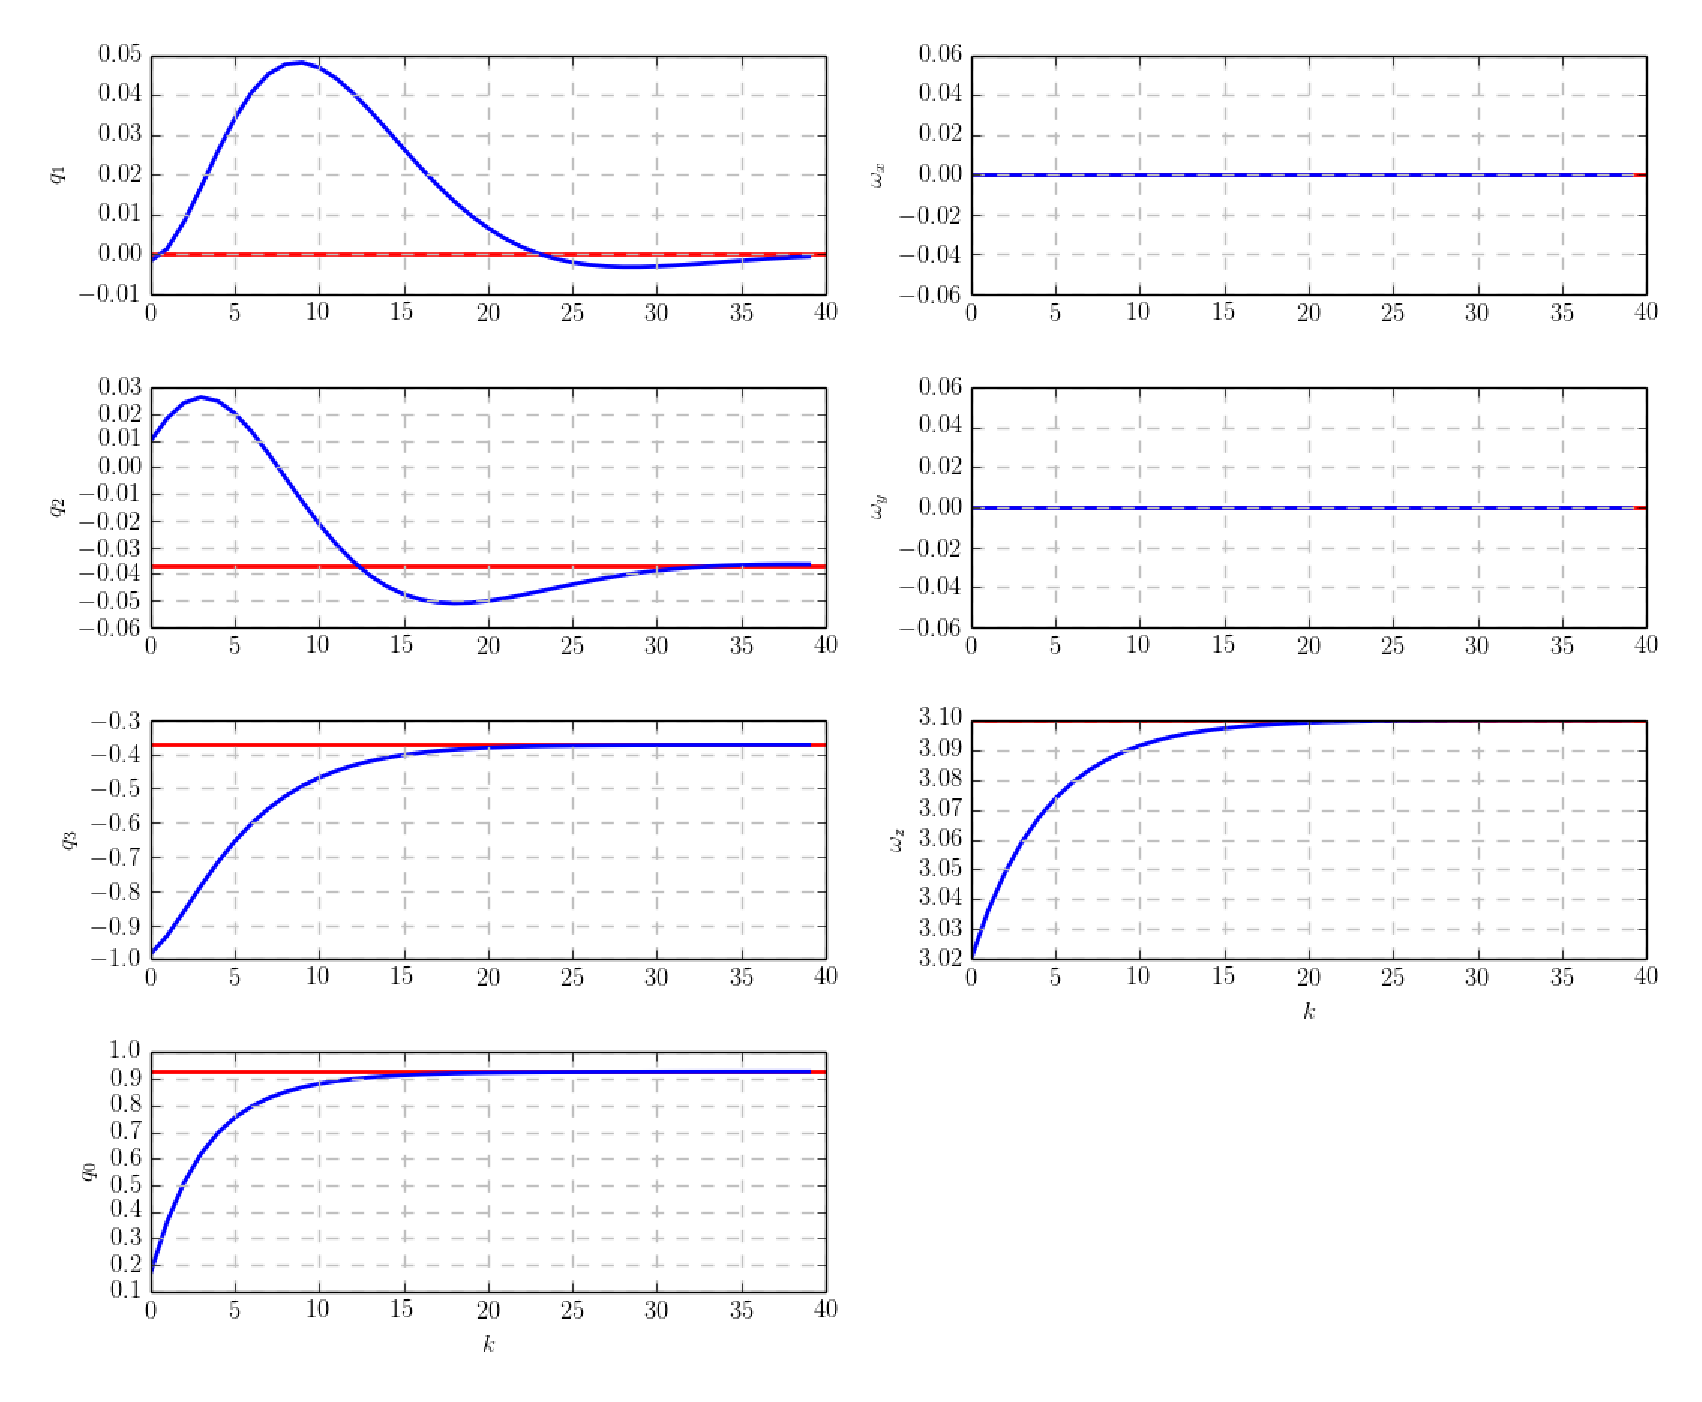
\psfig{file=figures/p_estimator_static_target.eps,width=6in}}
  \caption{P-Estimator with static target}
  \label{fig:PEstimatorwithstatictarget}
\end{figure}

The work covered so far in this chapter has all dealt with the a system in a static state.  In Figure \ref{fig:PEstimatorwithstatictarget}, a P-Estimator converges it's estimated state (blue) to the static measured state (red).  While the estimated state converges to the measured state after about 40 iterations, this type of conversion would be effective only for non-rotating systems.  The non-zero $\omega_z$ means that the quaternion attitude representation will be in constant motion.

The $3.1$ rad/sec rotation about $0\bs{i} + 0.1\bs{j} + 1\bs{k}$ condition from the previous p-estimator is then allowed to propagate the quaternion state through 10 second of rotation with state estimate updates every 0.1 sec.  The resulting measured state (red) and estimated state (blue) is shown in Figure \ref{fig:PEstimatorwithrotatingtarget}.  The body rates track identically to those in Figure \ref{fig:PEstimatorwithstatictarget} where $t(k) = 2$ corresponds to $k = 20$.  Due to the proportional only compensation and no predictive methods, the initial transient behavior is followed by a behavior similar to a steady state error.

\begin{figure}[H]
  \centerline{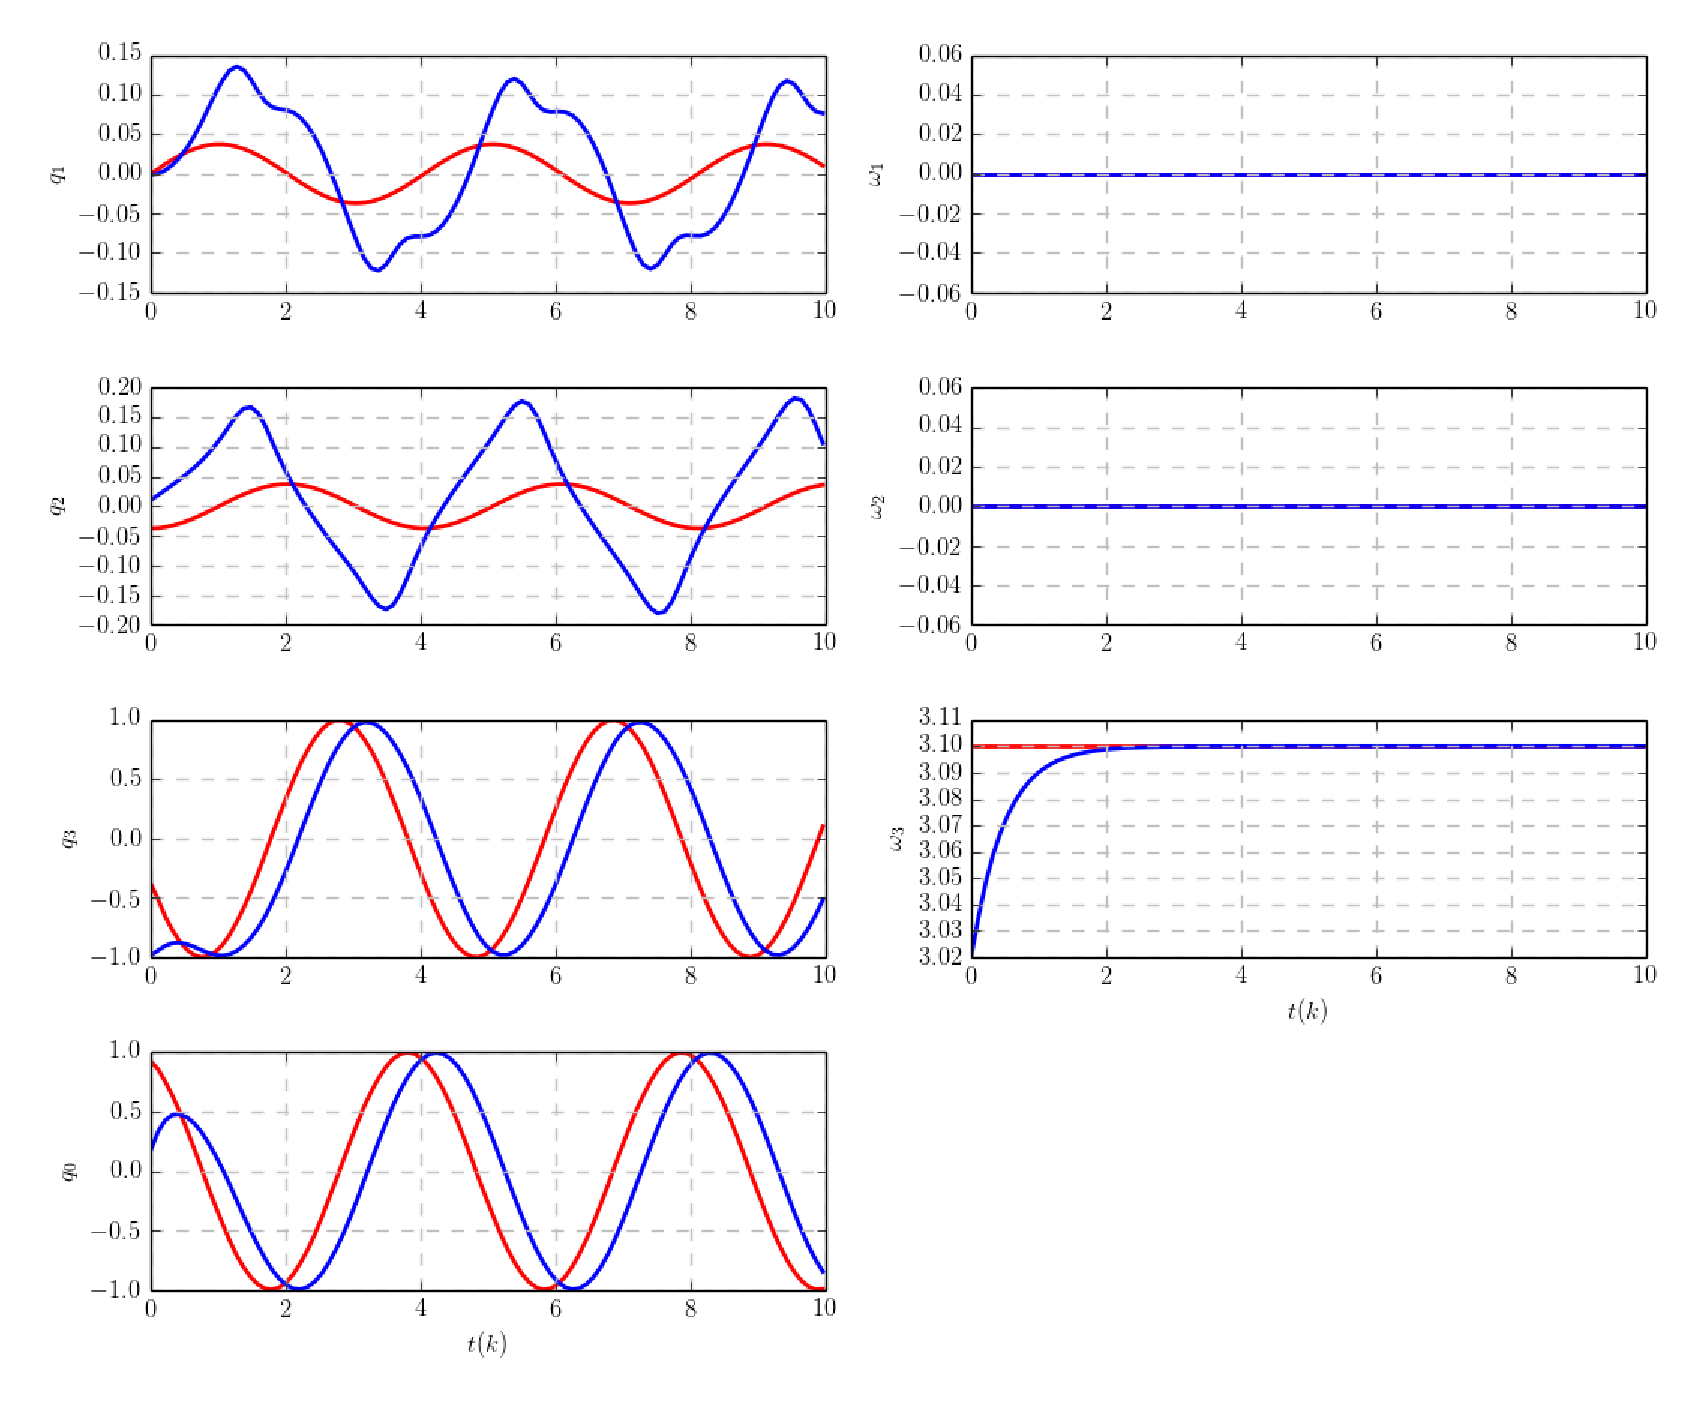
\psfig{file=figures/p_estimator_3radps.eps,width=6in}}
  \caption{P-Estimator with rotating target}
  \label{fig:PEstimatorwithrotatingtarget}
\end{figure}

Increasing the frequency of updates to the p-estimator can decrease the error between the measured and estimated states, but there will always be an error similar to a steady state error in the quaternion representation.  For better results the estimator needs to take into consideration changes in the state through the PID's integration and derivative terms.

\subsection{Integral State Estimation}
\label{subsec:IntegralEstimator}

To stay consistent with the findings in State Error (Chapter \ref{chap:StateError}), the quaternion portion of the integrated state should abide by the quaternion multiplicative correction method.  This is the first model where the variable sized time step is also taken into consideration.  Instead of accumulating the error measurements, the error corrections should be weighted according to the length of time between updates $t(k+1) - t(k)$.  In a simplified case the integral term should end up the same in the following two update instances.

\begin{table}[H]
  \centering
  \begin{tabular}{r|c|c|c|c|c}
    $t_1 (sec)$ & 0.1 & 0.2 & 0.3 & 0.4 & 0.5 \\ \hline
    $\theta_e$ & 4 & -3 & -3 & -3 & 5 \\
    \\
    $t_2 (sec)$ & 0.1 & & & 0.4 & 0.5 \\ \hline
    $\theta_e$ & 4 &  &  & -3 & 5 \\
  \end{tabular}
  \label{tbl:VariableUpdates}
\end{table}

In $t_1$, regular updates occur every 0.1 sec ending in an integral error value of 0.  In $t_2$, without taking into consideration the variable step sizes would end in an error value of $+6$, but really the -3 error update should be worth three times as much.

Running the state estimator without compensating for variations in time step sizes can create inconsistencies between different experimental runs.  In Figure \ref{fig:IEstimatorwithouttimevariationcompensation}, the integral estimator was updated with a fixed state for 30 seconds.  The estimator was initialized at $0$ radians and run three times against a fixed angle of $0.5$ radians.  The first time with an estimation update frequency of every 0.4 seconds (blue), second with the update frequency of every 0.1 seconds (red), and third with a variable update frequency (green) that jumped back and forth between updating every 0.05 and 0.4 seconds.

\begin{figure}[H]
  \centerline{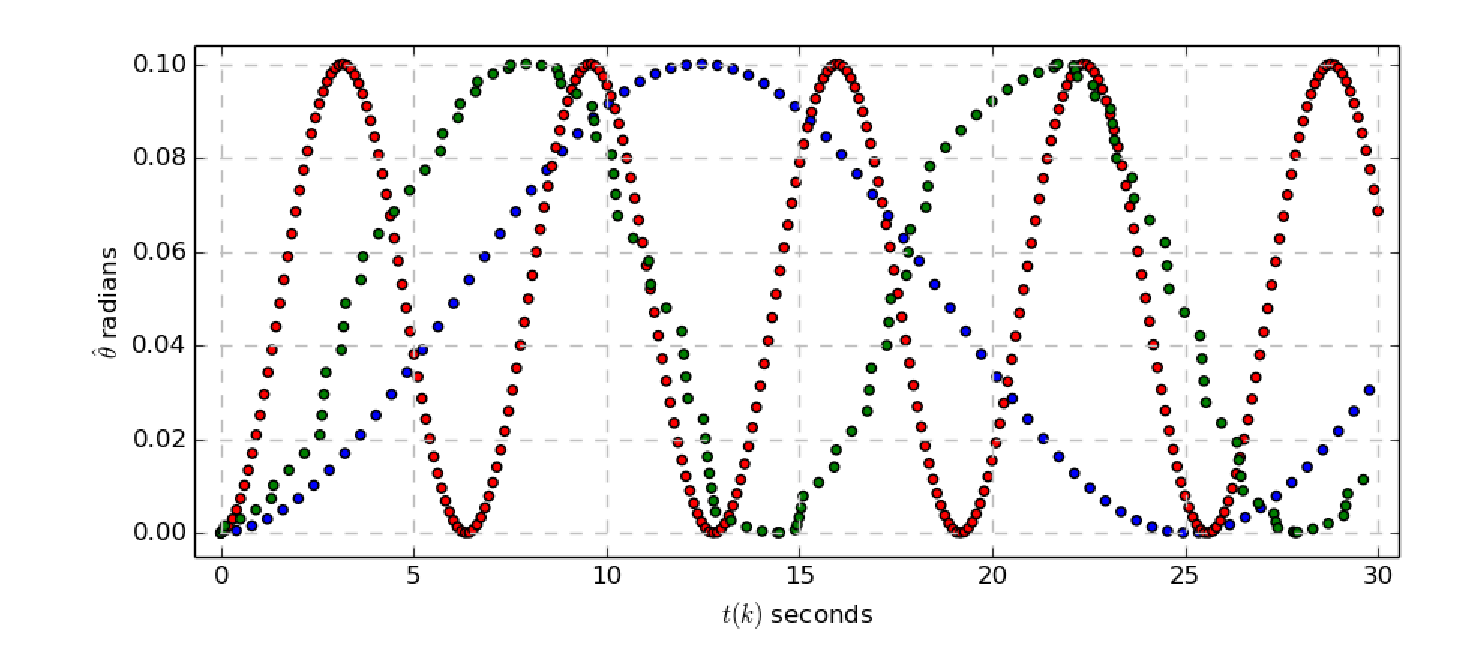
\psfig{file=figures/i_estimator_no_time_varying.eps,width=6in}}
  \caption{I-Estimator without time variation compensation}
  \label{fig:IEstimatorwithouttimevariationcompensation}
\end{figure}

Each calculated estimate for $\hat{\theta}$ in the $k$ domain is identical for each of the three runs, but varies greatly in the time domain.  Most notably, the third run that alternates between update frequencies ends up creating an estimation dynamic that could make the controller less robust.

In comparison, the PID estimator was modified to incorporate the time step size into it's integral term.  The same three tests were run as above with the 0.1 (red), 0.4 (blue), and variable 0.05/0.4 (green) time steps.  The adjustment quaternion method from Section \ref{sec:HighIntegrityStateAdjustments} is first used to compensate for measured time step size of $\Delta t_{k}$ creating a consistent error quaternion. then is used as before to scale the error quaternion by the selected gain value.  The results of this work can be seen in Figure \ref{fig:IEstimatorwithtimevariationcompensation} where the three test runs are still not identical, but their dynamics are more similar than before.  More notably, the variable step test (green) shows less variability in the estimate being produced which will reduce the noise being transferred to the control algorithm.

\begin{subequations}
  \begin{align}
    \bs{\hat{x}}(t_{k+1}) &= \begin{bmatrix} \bs{\hat{q}}(t_{k+1}) \\ \bs{\hat{\omega}}(t_{k+1}) \end{bmatrix} \\
    \bs{\hat{q}}(t_{k+1}) &= \bs{\psi}\big(\bs{q}_{ei}(t_k), K_{qi}\big) \otimes \bs{\hat{q}}(t_{k}) \\
    \bs{q}_{ei}(t_k) &= \bs{\psi}(\bs{q}_e(t_{k}), \Delta t_{k}) \otimes \bs{q}_{ei}(t_{k-1})\\
    \bs{\hat{\omega}}(t_{k+1}) &= \bs{\hat{\omega}}(t_{k}) + \bs{K}_{\omega i} \cdot (\Delta t_k \bs{I})\cdot \bs{\omega}_e(t_{k})
  \end{align}
  \label{eqn:IEstimator}
\end{subequations}

In Equation \ref{eqn:IEstimator}, the error quaternion $\bs{q}_{ei}(t_k)$ used is an accumulation of the time step scaled errors encountered in all previous steps.  This is analogous to a running summation of the error values.  For the body rate estimation, it's largely the traditional integral component with an extra $\Delta t_k \bs{I}$ term that linearly scales the body rate error calculations based on the size of the current time step.

\begin{figure}[H]
  \centerline{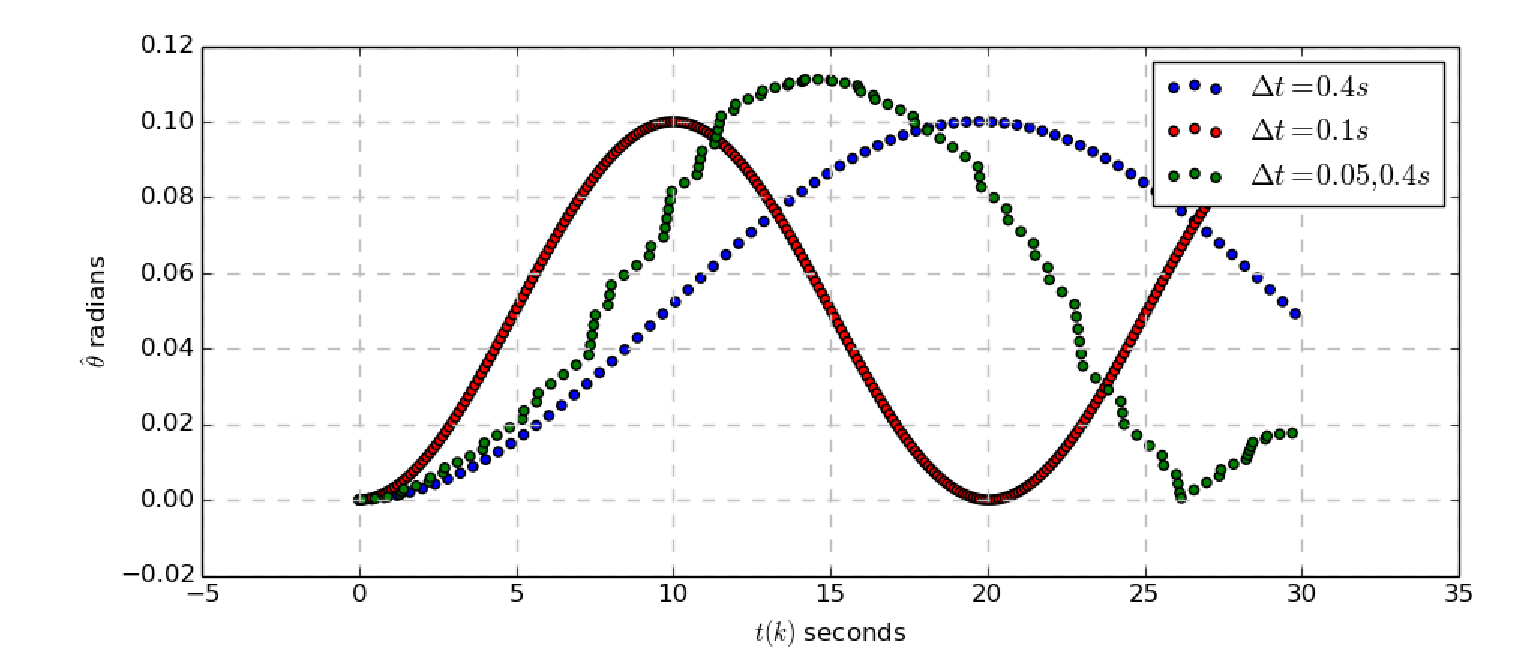
\psfig{file=figures/i_estimator_time_varying.eps,width=6in}}
  \caption{I-Estimator with time variation compensation}
  \label{fig:IEstimatorwithtimevariationcompensation}
\end{figure}

\subsection{Derivative State Estimation}
\label{subsec:DerivativeEstimator}

The derivative component of the PID estimator takes a similar form to the integral component in Equation \ref{eqn:IEstimator}.  The derivative component is only concerned with the current error, previous error, and the current time step size.  As with the integral body rate correction, the derivative correction is scaled by $\frac{1}{\Delta t_k}$ to compensate for variable step sizes.

\begin{subequations}
  \begin{align}
    \bs{\hat{x}}(t_{k+1}) &= \begin{bmatrix} \bs{\hat{q}}(t_{k+1}) \\ \bs{\hat{\omega}}(t_{k+1}) \end{bmatrix} \\
    \bs{\hat{q}}(t_{k+1}) &= \bs{\psi}\left(\bs{q}_{ed}(t_k), K_{qd}\right) \otimes \bs{\hat{q}}(t_{k}) \\
    \bs{q}_{ed}(t_k) &= \bs{\psi}\left(\bs{q}_e(t_{k-1})^* \otimes \bs{q}_e(t_{k}), \frac{1}{\Delta t_{k}}\right)\\
    \bs{\hat{\omega}}(t_{k+1}) &= \bs{\hat{\omega}}(t_{k}) + \bs{K}_{\omega d} \cdot \left(\frac{1}{\Delta t_k} \bs{I}\right) \cdot \bs{\omega}_e(t_{k})
  \end{align}
  \label{eqn:DEstimator}
\end{subequations}

The Figures \ref{fig:DEstimatorwithouttimevariationcompensation} and \ref{fig:DEstimatorwithtimevariationcompensation} below are the results of three test runs with the same set up update frequencies as with the integral component (0.1/sec, 0.4/sec, and varied).  For this comparison, the TableSat was simulated into a steady $0.01$ rad/s rotation about the body $+z$-axis to generate a constant rate of change for the quaternion instead of the fixed quaternion in the integral test.  The $\theta_{adj}$ parameter tracked for this test is the angular rotation associated with the $\bs{\psi}\left(\bs{q}_{ed}(t_k), K_{qd}\right)$ quaternion adjustment term.

\begin{figure}[H]
  \centerline{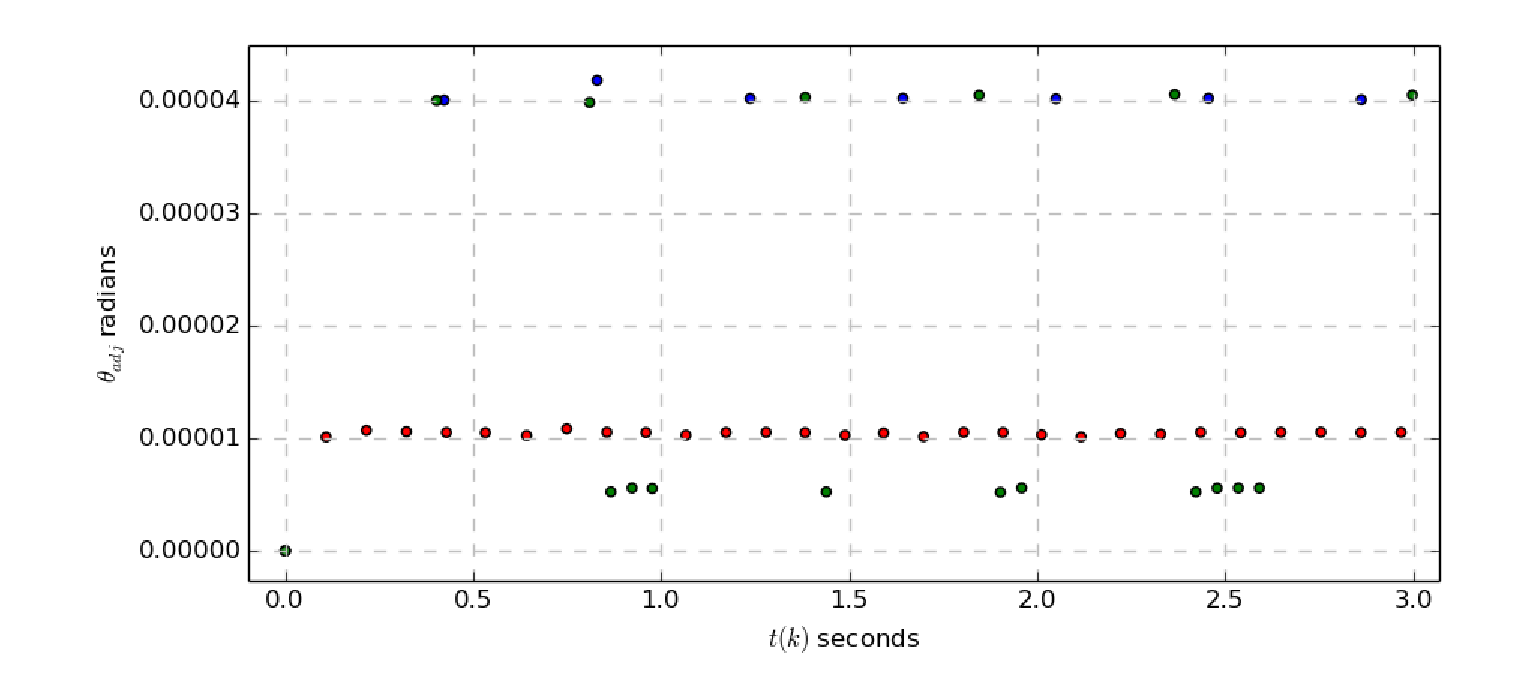
\psfig{file=figures/d_estimator_no_time_varying.eps,width=6in}}
  \caption{D-Estimator without time variation compensation}
  \label{fig:DEstimatorwithouttimevariationcompensation}
\end{figure}

Figure \ref{fig:DEstimatorwithouttimevariationcompensation} shows the results of the test run without consideration taken for time step sizes.  With a constant spin rate, the resulting quaternion adjustment is tightly coupled to the frequency that the updates are made with the 0.1 (red), 0.4 (blue), and variable 0.05/0.4 (green) time steps.  The variable time step sequence is a particular concerns as it jumps back and forth between adjusted amount suggesting the spin rate is not constant.

\begin{figure}[H]
  \centerline{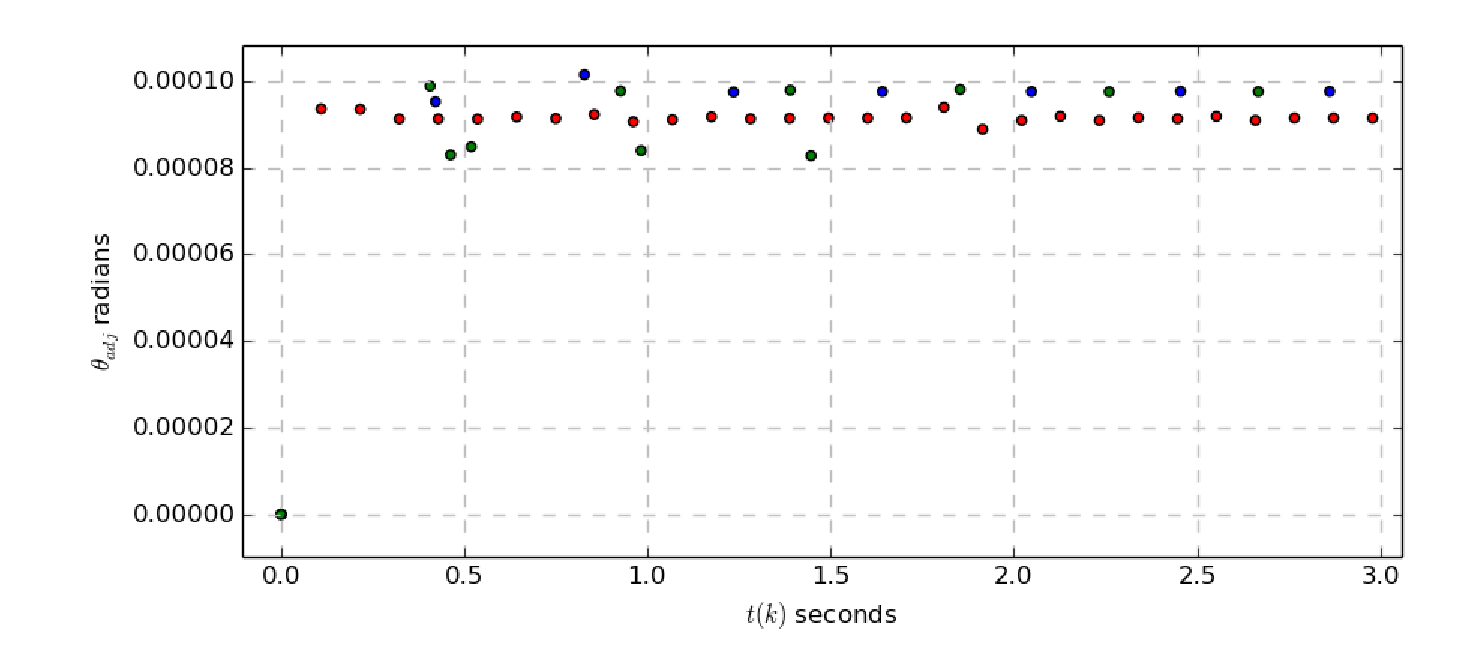
\psfig{file=figures/d_estimator_time_varying.eps,width=6in}}
  \caption{D-Estimator with time variation compensation}
  \label{fig:DEstimatorwithtimevariationcompensation}
\end{figure}

Figure \ref{fig:DEstimatorwithtimevariationcompensation} implements the time variation compensation in Equation \ref{eqn:DEstimator} where the quaternion adjustments provide a better representation of the measured constant spin rate.

\subsection{PID State Estimation of Unforced Motion}
\label{subsec:PIDEstimatorofUnforcedMotion}

Combining the proportional, integral, and derivative estimator portions from above.  Equations \ref{eqn:PEstimator}, \ref{eqn:IEstimator}, and \ref{eqn:DEstimator} get combined into a single PID estimator as

\begin{subequations}
  \begin{align}
    \bs{\hat{x}}(t_{k+1}) &= \begin{bmatrix} \bs{\hat{q}}(t_{k+1}) \\ \bs{\hat{\omega}}(t_{k+1}) \end{bmatrix} \\
    \bs{\hat{q}}(t_{k+1}) &= \bs{\psi}\left(\bs{q}_{ed}(t_k), K_{qd}\right) \otimes \bs{\psi}\big(\bs{q}_{ei}(t_k), K_{qi}\big) \otimes \bs{\psi}(\bs{q}_e(t_{k}), K_{qp})  \otimes \bs{\hat{q}}(t_{k}) \\
    \bs{\hat{\omega}}(t_{k+1}) &= \bs{\hat{\omega}}(t_{k}) + \bs{K}_{\omega p} \cdot \bs{\omega}_e(t_{k}) + \bs{K}_{\omega i} \cdot (\Delta t_k \bs{I})\cdot \bs{\omega}_e(t_{k}) + \bs{K}_{\omega d} \cdot \left(\frac{1}{\Delta t_k} \bs{I}\right) \cdot \bs{\omega}_e(t_{k})
  \end{align}
  \label{eqn:PIDEstimatorUnforcedMotion}
\end{subequations}

The update to the estimated body rate follows the traditional method of the PID control with the addition of the scaling factors for the integral and derivative terms that compensate for non-uniform step sizes at run-time.  The quaternion correction is a compilation of the individual correction quaternions and joined through the multiplicative error correction method.

With a spin-stabilized system controlling the body rate is relatively straight forward with a PID controller.  A test was run through TSatPy with based on the PID estimation in Equation \ref{eqn:PIDEstimatorUnforcedMotion}.  The system was set at a spin rate of $0.314$ rad/sec rotation about $+z$ with the measurement of the quaternion angle $\theta$ containing noise $N \sim (0, 0.1218)$ radians.  A gradient descent gain selection settled on the following parameters.

\begin{equation}
  \begin{aligned}
    K_{qp} &= 0.98, K_{qi} = 0.001, K_{qd} = 0.001 \\
    \bs{K}_{\omega p} &= 0.7 \bs{I}, \bs{K}_{\omega i} = \bs{0}, \bs{K}_{\omega d} = \bs{0}
  \end{aligned}
\end{equation}

The test run results are show in Figure \ref{fig:PIDEstimatorwithoutstateprediction}.  The bottom two graphs showing body rate tracking performance where the basic proportional control quickly brings the body rate error under control.  The quaternion estimations are much more difficult largely due to the lack of a system model to convert body rates to estimated attitudes at the next update.  Since the system is spin-stabilized and the estimated quaternion has no prior knowledge of where the next value will be, it relies on a large proportional component to jump to the new measurement values on each update.

While testing the performance of the integral and derivative components showed an improved performance when incorporating the effects of the variable time step, in this test with such a heavy reliance on the proportional component, the benefits to considering the variable time step effects were negligible.

\begin{figure}[H]
  \centerline{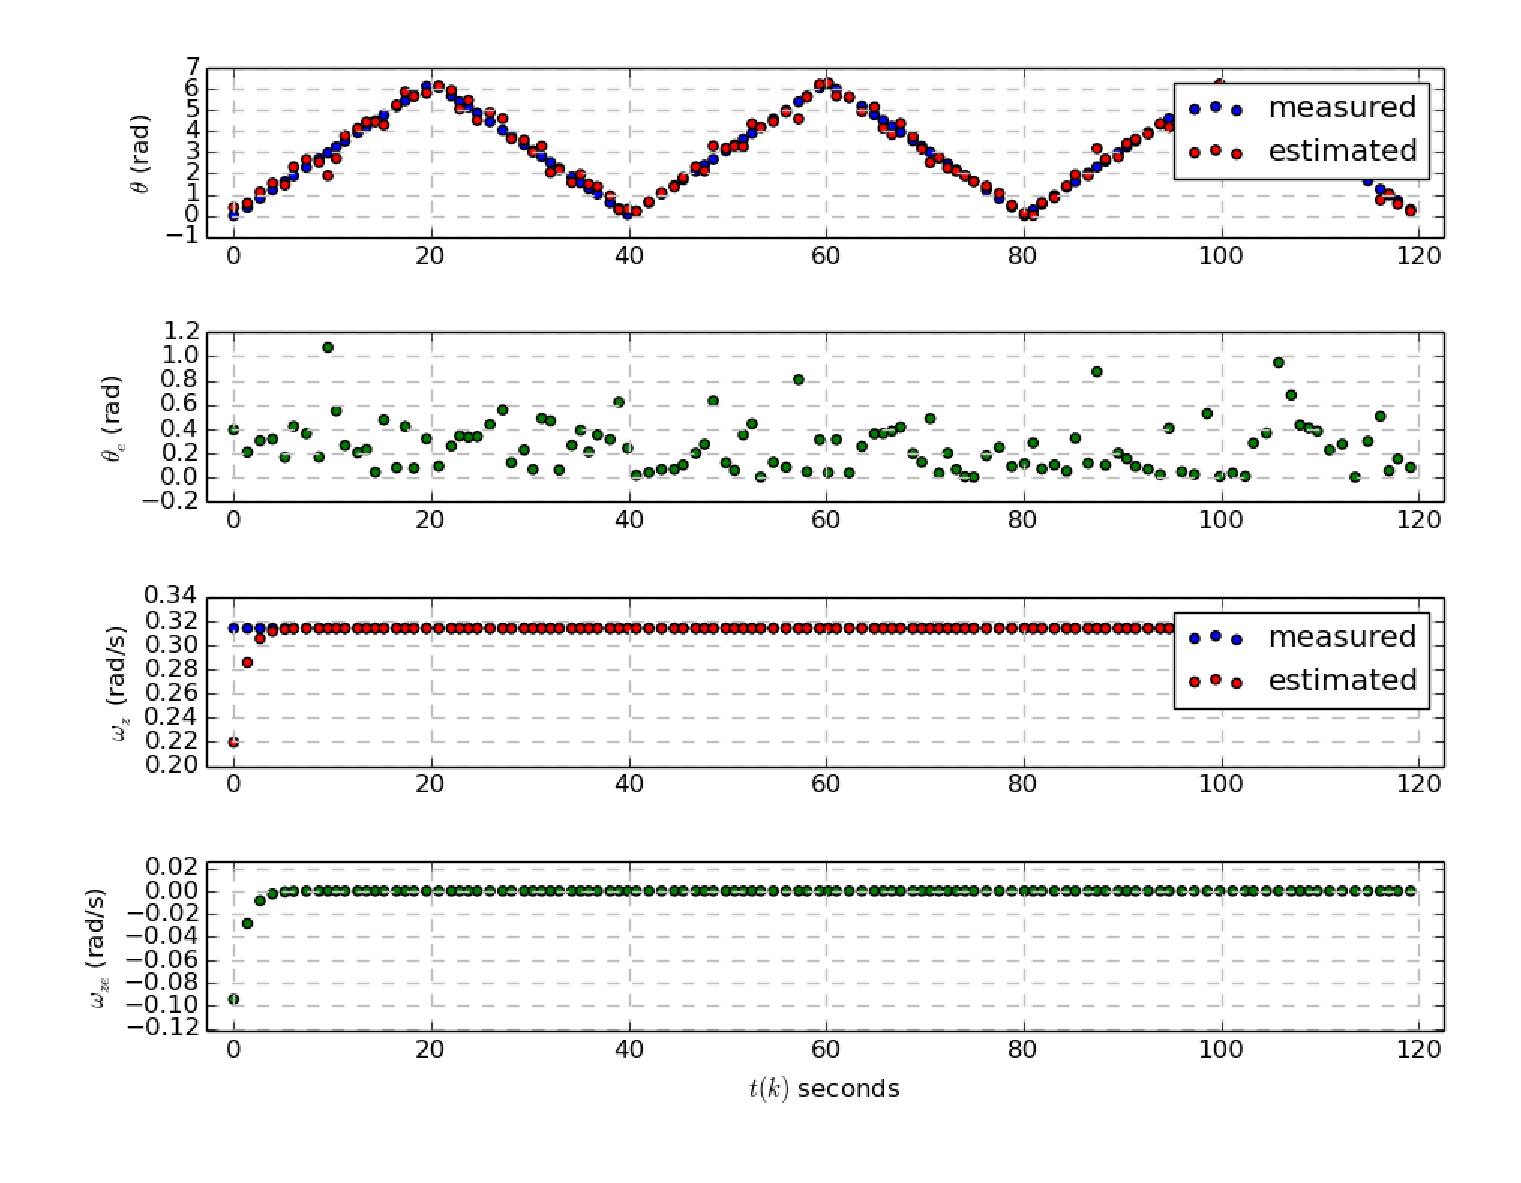
\psfig{file=figures/pid_estimator_no_prediction_high_P.eps,width=6in}}
  \caption{PID-Estimator without state prediction}
  \label{fig:PIDEstimatorwithoutstateprediction}
\end{figure}


\subsection{PID Estimation with State Prediction}
\label{subsec:PIDEstimatorwithStatePrediction}

From Section \ref{sec:BodyRatePIDEstimation}, Equation \ref{eqn:PIDEstimatorUnforcedMotion} defines a method of tracking unforced spin-stabilized satellites through PID state estimation.  The biggest issue was a heavy reliance on the proportional gain to track the quaternion attitude which is sensitive to measurement noise.  Incorporating a multiplicative-correction quaternion based model of rigid body dynamics based on the equations in Chapter \ref{chap:SatelliteAttitudeDynamicsAndKinematics} can assist in predicting the $t_{k+1}$ state of the system.

\begin{subequations}
  \begin{align}
    \bs{\hat{x}}(t_{k+1}) &= \begin{bmatrix} \bs{\hat{q}}(t_{k+1}) \\ \bs{\hat{\omega}}(t_{k+1}) \end{bmatrix} \\
    \bs{\hat{q}}(t_{k+1}) &= \bs{\psi}\left(\bs{q}_{ed}(t_k), K_{qd}\right) \otimes \bs{\psi}\big(\bs{q}_{ei}(t_k), K_{qi}\big) \otimes \bs{\psi}(\bs{q}_e(t_{k}), K_{qp})  \otimes \bs{\hat{q}}(t_{k+1})^- \\
    \bs{\hat{\omega}}(t_{k+1}) &= \bs{\hat{\omega}}(t_{k+1})^- + \bs{K}_{\omega p} \cdot \bs{\omega}_e(t_{k}) + \bs{K}_{\omega i} \cdot (\Delta t_k \bs{I})\cdot \bs{\omega}_e(t_{k}) + \bs{K}_{\omega d} \cdot \left(\frac{1}{\Delta t_k} \bs{I}\right) \cdot \bs{\omega}_e(t_{k})
  \end{align}
  \label{eqn:PIDEstimatorwithPredictionUnforcedMotion}
\end{subequations}

with the a priori state $\bs{\hat{x}}(t_{k+1})^-$ as

\begin{equation}
  \bs{\hat{x}}(t_{k+1})^- = \begin{bmatrix}\bs{\hat{q}}(t_{k+1})^- \\ \bs{\hat{\omega}}(t_{k+1})^- \end{bmatrix} = f \Big( \bs{\hat{q}}(t_{k}), \bs{\hat{\omega}}(t_{k}) \Big)
\end{equation}

The PID estimator now with a state prediction method was run under the same testing conditions present in Figure \ref{fig:PIDEstimatorwithoutstateprediction}.  The resulting performance showed that the inclusion of the system model greatly reduced the reliance on the proportional component of the PID estimator which reduced the noise and increased the accuracy of the final estimates being provided to the controller.  The results in Figure \ref{fig:PIDEstimatorwithstateprediction} show the improved quaternion angle estimates when run with the following gains.

\begin{equation}
  \begin{aligned}
    K_{qp} &= 0.0735, K_{qi} = 0.000863, K_{qd} = 0.00812 \\
    \bs{K}_{\omega p} &= 0.7 \bs{I}, \bs{K}_{\omega i} = \bs{0}, \bs{K}_{\omega d} = \bs{0}
  \end{aligned}
\end{equation}

The quaternion's proportional value is still the dominant gain, but has been reduced by 92.5\% of it's previous value while still providing about 80\% reduction in quaternion attitude error rates.

\begin{figure}[H]
  \centerline{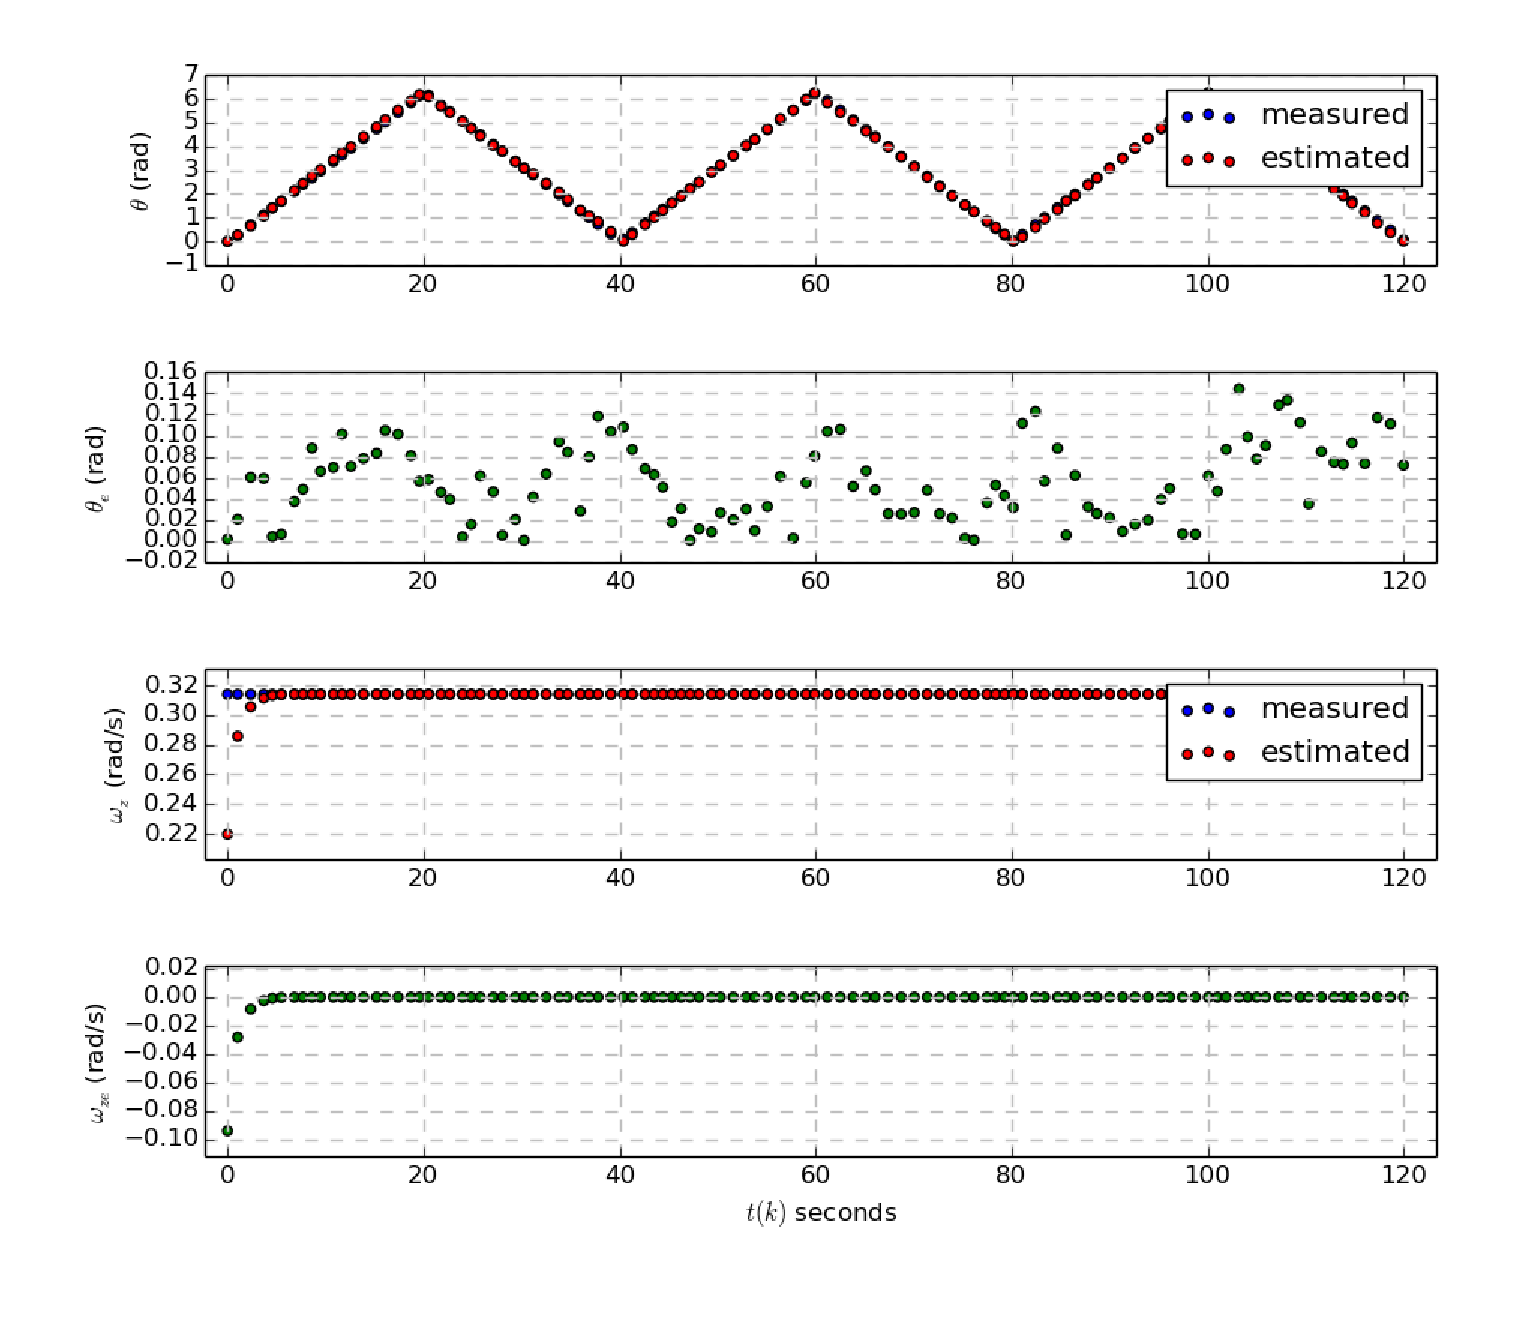
\psfig{file=figures/pid_estimator_with_prediction.eps,width=6in}}
  \caption{PID-Estimator with state prediction}
  \label{fig:PIDEstimatorwithstateprediction}
\end{figure}


\section{Sliding Mode Observer with State Prediction}
\label{sec:SlidingModeObserverwithStatePrediction}

The Sliding Mode Observer (SMO) is a proportional estimator with an additional smoothing term that uses a chosen sliding surface.  The general form for the SMO is

\begin{equation}
  \bs{\dot{\hat{x}}} = \bs{\hat{f}}(\bs{\hat{x}}, \bs{\hat{u}}, t) + \bs{L}(\bs{C}\bs{\hat{x}} - \bs{C}\bs{x}) + \bs{K}\bs{1}_s\bs{\hat{y}}
  \label{eqn:SMOContinuous}
\end{equation}

Where L is a luenberger gain and $\bs{1}_s$ is a switching function based on $s$.  The sliding mode terms allow additional control of the state adjustments without adding a lot of computational complexity.  The SMO can continue to use the nonlinear model's state predictions as in the PID estimators in Section \ref{subsec:PIDEstimatorwithStatePrediction}, which is an advantage over methods such as the Extended Kalman Filter (EKF) where the system is linearized about an operating point and assumes a constant time step.

This thesis takes the discretized form of Equation \ref{eqn:SMOContinuous} with a quaternion multiplicative correction

\begin{subequations}
  \begin{align}
    \bs{\hat{x}}(t_{k+1}) &= \begin{bmatrix} \bs{\hat{q}}(t_{k+1}) \\ \bs{\hat{\omega}}(t_{k+1}) \end{bmatrix} \\
    \bs{\hat{q}}(t_{k+1}) &= \bs{\psi} (\bs{1}_s\big(\bs{q}_{e}(t_k)\big), K_q) \otimes \bs{\psi}(\bs{q}_e(t_{k}), L_{q})  \otimes \bs{\hat{q}}(t_{k+1})^- \\
    \bs{\hat{\omega}}(t_{k+1}) &= \bs{\hat{\omega}}(t_{k+1})^- + \bs{L}_{\omega} \bs{\omega}_e(t_{k}) + \bs{K}_{\omega}\bs{1}_s \big(\bs{\omega}_e(t_{k}) \big)
  \end{align}
  \label{eqn:SMOEstimatorwithPredictionUnforcedMotion}
\end{subequations}

where

\begin{subequations}
  \begin{align}
    \bs{1}_s\big(\bs{q}_{e}(t_k) \big) &= \begin{bmatrix} \bs{v_e} \\ sat\left( \frac{2\cos^{-1} q_{0e} }{S_{q}} \right) \end{bmatrix} \\
    \bs{1}_s \big(\bs{\omega}_e(t_{k}) \big) &= sat\left( \frac{\bs{\omega}_e(t_{k})}{S_{\omega}} \right) \\
    \bs{L}_{\omega} &= L_\omega \cdot \bs{I} \\
    \bs{K}_{\omega} &= K_\omega \cdot \bs{I}
  \end{align}
\end{subequations}

For body rates, the a priori state provides the predicted body rate $\bs{\hat{\omega}}(t_{k+1})^-$ that gets adjusted by a proportional term $\bs{L}_{\omega} \bs{\omega}_e(t_{k})$ as in the P-Estimator, but has an additional saturation function correction based on sliding surfaces for the individual body rate errors.  As found in the PID estimator, the proportional estimator for a steady spin-stabilized satellite performs adequately.  The additional saturation term becomes helpful for situations with low $L_\omega$ values that can take longer to converge from the initial body rate to the actual body rate, but once close will increase the effort in staying in step with the measured body rate.

Similar to the PID estimator, the quaternion sliding mode observer limits it's focus to the angular measure of the rotational quaternion.  The sliding surface is taken based on the radian measure.  If the radian measure is below, the saturation limit the quaternion stays as is.  If the quaternion represents a rotation greater than the saturation limit a saturated quaternion is created about the same Euler axis but limit to the saturation angle of rotation.

Running the same tests as run against the PID estimators, the following parameters were located through an iterative gradient descent method that minimized the quaternion error angle and standard deviation of the error angle.

\begin{equation}
  \begin{aligned}
    L_q = 0.362 &, L_w = 0.375 \\
    K_q = 0.308 &, K_w = 0.499 \\
    S_q = 0.419 &, S_w = 0.00517 \\
  \end{aligned}
\end{equation}

Figure \ref{fig:SMOEstimatorwithstateprediction} shows the result of the test at these optimized parameters.  The inverted angle measurement in the first graph is an artifact of the non-unique representation of a quaternion attitude.  In this case, the estimated angles are being calculated for rotations about the body's $-z$-axis instead of the $+z$ axis.  This further supports the decision made in Section \ref{chap:StateError} to use the multiplicative error as the second graph shows the correct error values.

Although the SMO in this case is able to traverse the initial transient response well, the steady state quaternion error is almost as high as using a PID estimator with no state prediction method.  This behavior is due to the high quaternion measurement noise.  With the saturation function, the sliding mode observer is still largely a proportional estimator without the assistance of an integral term to smooth out the noise.

\begin{figure}[H]
  \centerline{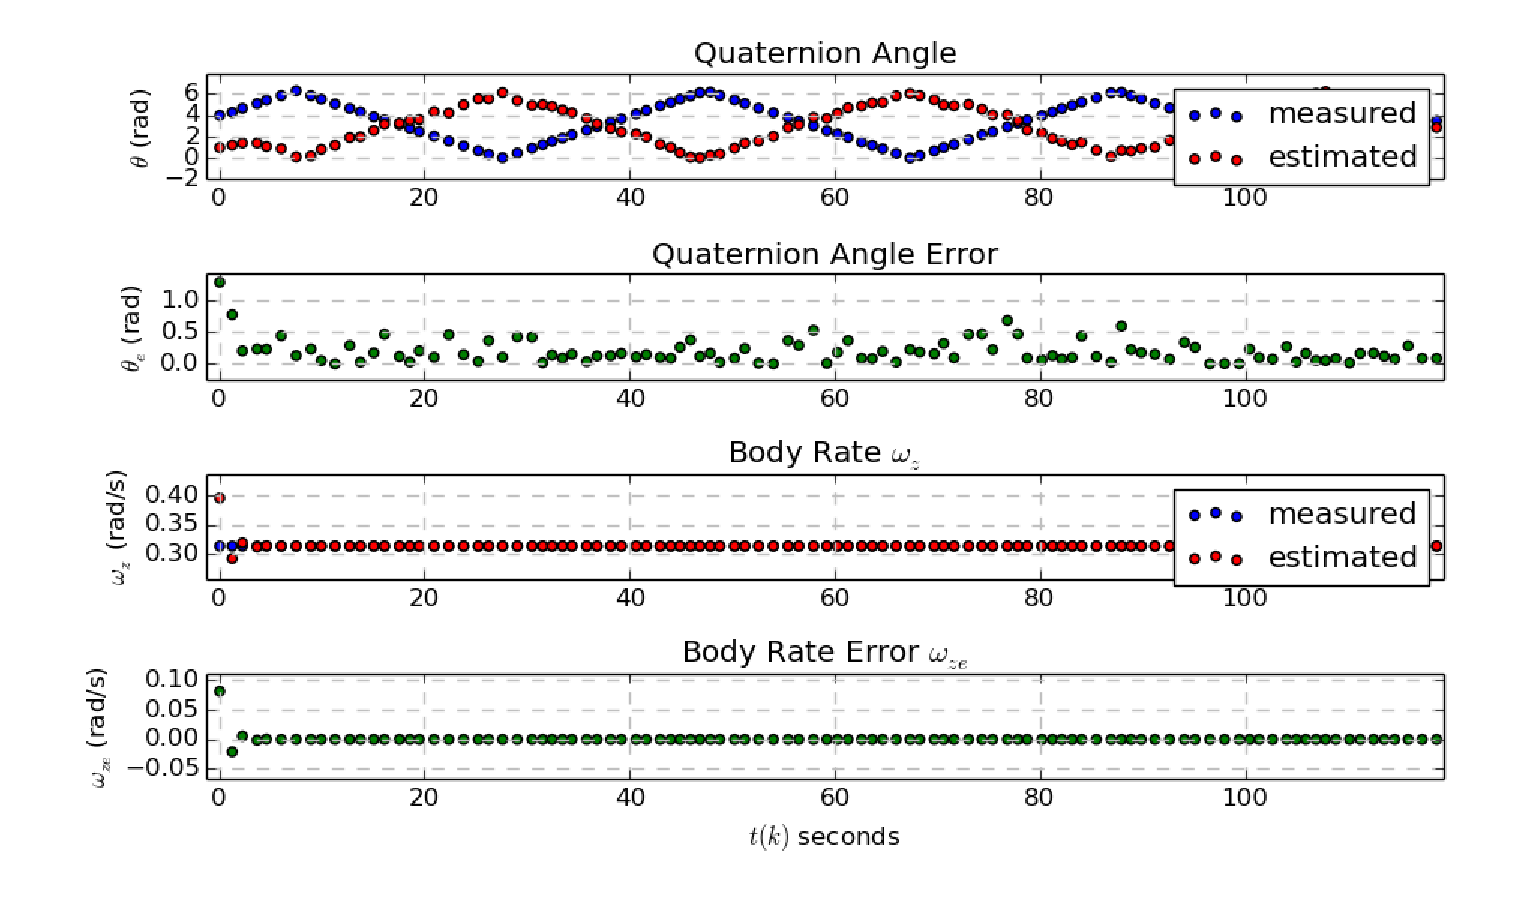
\psfig{file=figures/smo_estimator_with_prediction.eps,width=6in}}
  \caption{SMO-Estimator with state prediction}
  \label{fig:SMOEstimatorwithstateprediction}
\end{figure}

Based on these results, the SMO performs acceptably for the body rate estimation, but according to the steady state error rates, it appears that the PID estimation would be a better use for the steady state attitude tracking.  Both estimators have similar performance profiles which makes it more complicated to determine the better choice.  Section \ref{sec:ComparativeAnalysysofPIDandSMOEstimators} will go over how TSatPy can assist with running both estimation techniques in parallel for to provide a more accurate representation.

\section{Comparative Analysis of PID and SMO Estimators}
\label{sec:ComparativeAnalysysofPIDandSMOEstimators}

One of the advantages to developing the TSatPy code base for the MMS/TableSat spin-stabilized is the ability to run a comparative analysis of multiple estimators at the same time.  The estimators run agnostic to the source of the measurements.  In the sample shown below, the state measurements were generated by a model, but could also be switched to be pulled off the TableSat.

Figure \ref{fig:PIDSMOEstimatorConcurrentComparison} was generated by running a single simulation an providing the truth model's measured state to both a PID and SMO estimator tuned to the parameters selected during individual gain tuning tests above.  This allows for a clear side-by-side comparison of their performance.  Multiple runs all have similar characteristics.  In the initial transient response both estimators are able to converge to a steady state after just a couple updates, but the SMO is able to converge slightly faster each time.  For the steady state response the PID estimator consistently maintains a lower average error, although with a slightly higher standard deviation.  As with the initial response, the SMO estimation values generally update slightly just before the PID estimator.

\begin{figure}[H]
  \centerline{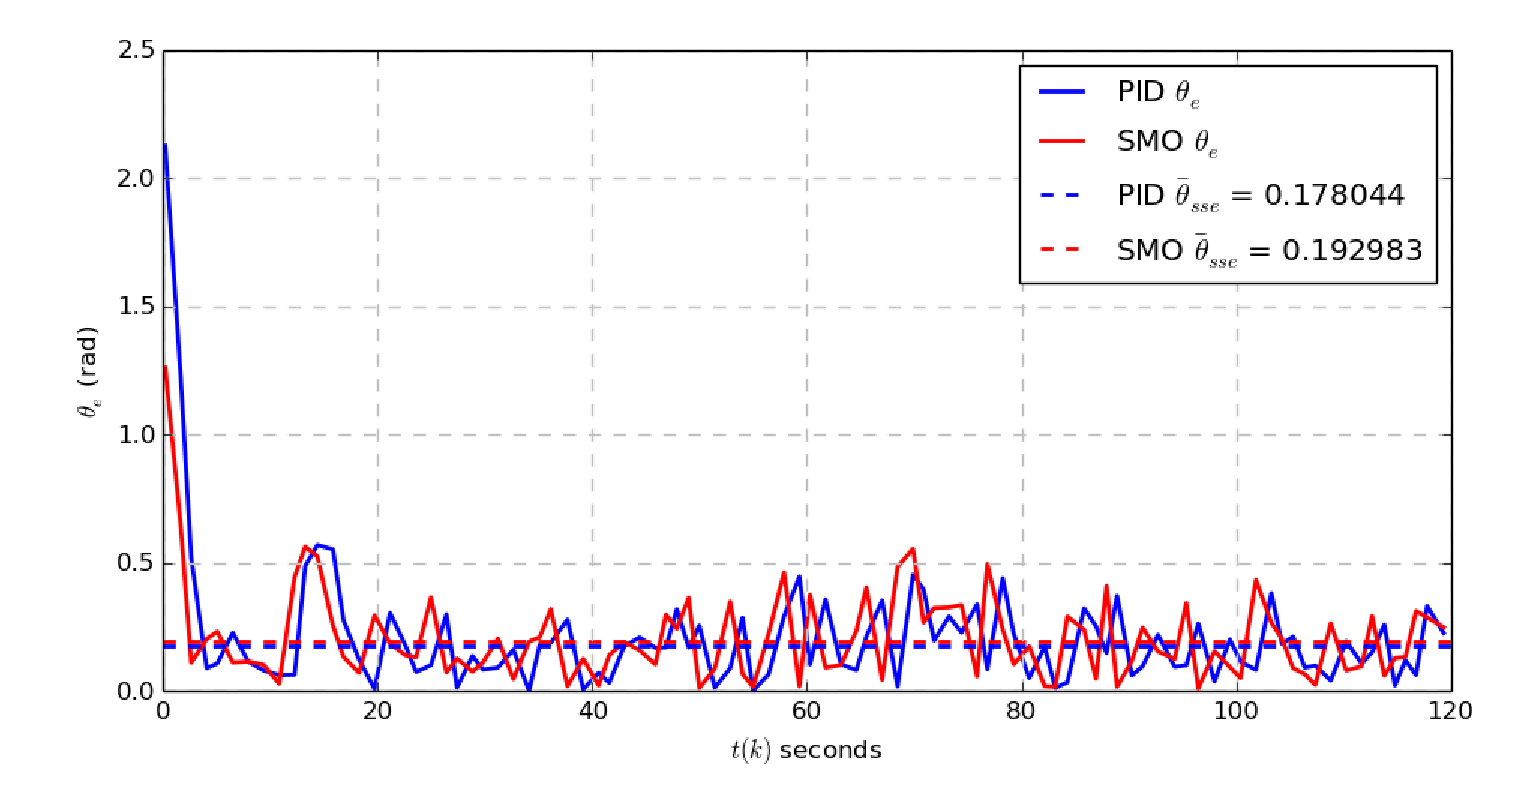
\psfig{file=figures/estimator_comparison.eps,width=6in}}
  \caption{PID/SMO Estimator Concurrent Comparison}
  \label{fig:PIDSMOEstimatorConcurrentComparison}
\end{figure}

The results in Figure \ref{fig:PIDSMOEstimatorConcurrentComparison} were generated through the TSatPy application with the script below.  Lines 10-15 define the two estimators to use in the simulation.  More can be added including the same estimator type with varied parameters.  Lines 17-19 define the system clock behavior.  The simulation will run for a simulated 120 seconds as verified in the results above.  The time steps for each update will vary between 0.8 and 1.2 seconds randomly.  And since this is running as a simulation instead of pulling data from the physical TableSat, the clock can be sped up to run at 10x speed improving the rate of the iterative testing cycle.

\begin{singlespace}
  \begin{minted}[mathescape,linenos,numbersep=10pt,frame=lines,framesep=2mm]{python}
from TSatPy import Estimator, State
from TSatPy.Clock import Metronome
import numpy as np
import matplotlib.pyplot as plt
import time
import random

print('PID / SMO Faceoff')

configs = [{'type': 'pid',
 'args': {'kpq': 0.0735,'kpw': 0.7,'kiq': 0.000863,
          'kiw': 0,'kdq': 0.00812,'kdw': 0}
},{'type': 'smo',
 'args': {'Lq': 0.3619,'Lw': 0.3752,'Kq': 0.3076,
           'Kw': 0.4994,'Sq': 0.4191,'Sw': 0.0052}}]

run_time = 120
speed = 10
dts = [0.8, 1.2]
c = Metronome()
c.set_speed(speed)
I = [[2, 0,  0], [0, 2, 0], [0, 0, 2]]

def setup_estimators(configs):
    x_ic = State.State()
    plant_est = State.Plant(I, x_ic, c)

    est = Estimator.Estimator(c)
    for config in configs:
        est.add(config['type'], plant_est, config['args'])

    return est

def run_comparison(est):
    x_ic = State.State(
        State.Quaternion([0,0,1], radians=4),
        State.BodyRate([0,0,0.314]))
    plant = State.Plant(I, x_ic, c)

    ts = []; smo_err = []; pid_err = []
    start_time = c.tick()
    end_time = c.tick() + run_time
    while c.tick() < end_time:
        plant.propagate()
        offset = np.random.randn() * 20 / 180.0 * np.pi
        q_noise = State.Quaternion([0,0,1], radians=offset) * plant.x.q

        x_m = State.State(q_noise, plant.x.w)

        est.update(x_m)
        ts.append(c.tick() - start_time)

        for model in est.estimators:
            q_e = State.QuaternionError(model.x_hat.q, plant.x.q)
            e, r = q_e.to_rotation()

            if type(model) is Estimator.PID:
                pid_err.append(r)
            elif type(model) is Estimator.SMO:
                smo_err.append(r)
        random.shuffle(dts)
        time.sleep(dts[0] / float(speed))

    return ts, pid_err, smo_err

def graph_it(ts, pid_err, smo_err):
    # Generate the graph here
    # See appendix for the full script

def main():
    est = setup_estimators(configs)
    graph_it(*run_comparison(est))
    return 0

if __name__ == '__main__':
    exit(main())
  \end{minted}
\nocite{minted}
\end{singlespace}

The TableSat 1A controller has performance requirements based off of NASA MMS's mission parameters.  Section \ref{sec:ComparativeAnalysysofPIDandSMOEstimators} demonstrated that multiple estimators can be run in parallel during both simulations and experimental runs.  As discussed above, this allows for a better insight into performance differences in estimation methods.  An additional benefit to running the controller through TSatPy is the ability to perform estimator scheduling.  Like gain scheduling which for an estimator or controller can modify what gains it uses depending on the current performance, estimator scheduling allows for switching between disparate estimation techniques during run-time.  For example, one estimator tuned for responding to large errors and run along side an estimator tuned for steady state performance.  The control algorithm can then receive more accurate state estimates on a wider range of environmental conditions.


\chapter{CONTROLLERS}
\label{chap:Controllers}

The control requirements for NASA MMS TableSat 1A can be simplified into three main goals.

First is to maintain a steady spin rate of 3 rpm ($\pi/10$ rad/sec).  Given the relative success of the body rate estimation in Section \ref{chap:Estimators}, this goal should be attainable without the need of advanced control efforts.

Second is to correct for any nutation detected by the estimator.  This requirement can take the form of both driving body rates $\omega_y$ and $\omega_z$ to zero, and ensuring the estimated quaternion's Euler axis is kept in line with the global reference frame's $z$-axis.

Third is to prevent and/or remove oscillations in the Axial Double Probe (ADP) and Spin-plane Double Probe (SDP) booms.  Out of the three, this performance goal has the largest set of dependencies for success.  This level of control is reliant on effective actuators along with reliable state estimates based on an accurate system model which include boom dynamics.

The first two goals is addressed in this chapter as their scope is limited to controller design.  Section \ref{sec:ActuatorConfiguration} covers the configuration of the actuators on TableSat and how their configuration is incorporated into the controller code.  The remaining sections of this chapter focus on the rate and nutation control methods, and use the assumption that the estimators are providing perfect state measurements.  This temporarily limits the scope of the testing to ensure that the control techniques are being implemented properly in the software especially since with the development of some non-standard techniques.  The boom oscillations control goal is addressed in Chapter \ref{chap:ObserverBasedControls} when multiple modules are be linked together to get a wider view of the interactions between sections of observer-based controller acting on noisy state measurements.

\section{Actuator Configuration}
\label{sec:ActuatorConfiguration}

The actuators in use on NASA MMS TableSat 1A consists of four single directional computer fans.  Two oriented for rate control and two for nutation control.  The body rate control fans are mounted on opposite sides of the bus with their thrusts applying opposing moments.  The two nutation fans are mounted flush with the bus at a 90 degree offset and have their thrust directed down.  The fans are assumed to be mounted such that the moments are applied about orthogonal axes.  This simplifies the actuator module's voltage calculations for each fan which can be improved if testing shows the effects are significant enough to compensate for.  Four analog ports to the Athena PC are available for actuator usage after mounting the sensors.  Two dedicated to the rotational fans to provide full rotational control, and the remaining two provide partial nutation control.
\begin{figure}[H]
  \centerline{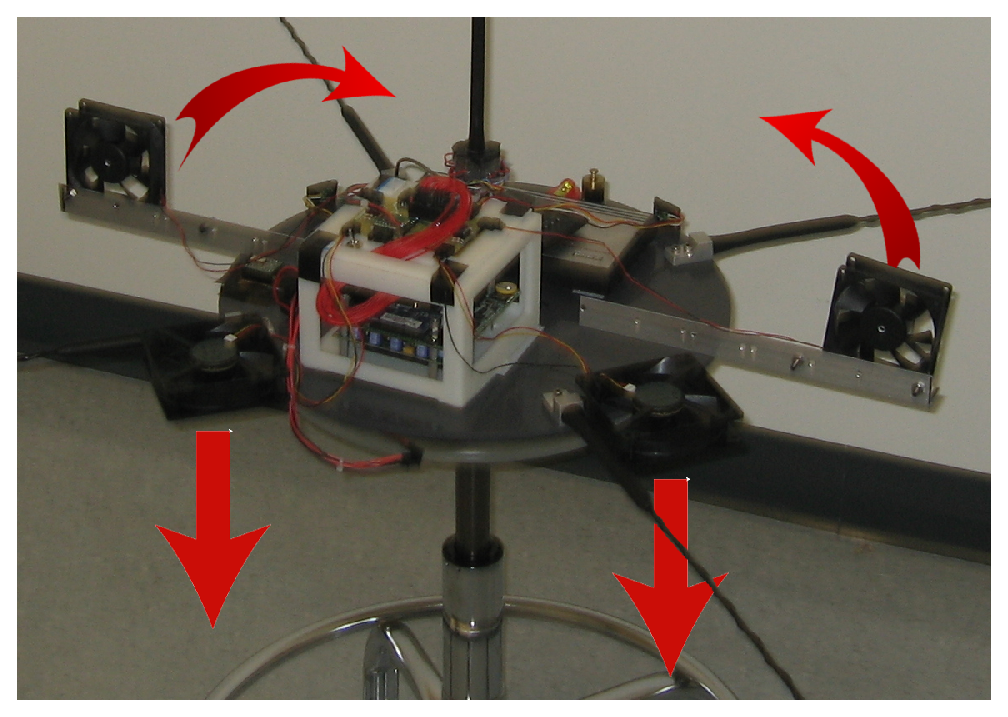
\psfig{file=figures/tsat_thrusters.eps,height=3in}}
  \caption{NASA MMS TableSat 1A thrusters}
  \label{fig:TSatThrusters}
\end{figure}
Passing the desired moments from the controller directly to the estimator without taking the fan geometry into consideration would create a disconnect between the estimated and actual system states.  The software's actuator module is designed to accept a list of fans with their center, direction of thrust related to the body reference frame, and maximum force to determine the moments couples that are actually possible.
\begin{figure}[H]
  \centerline{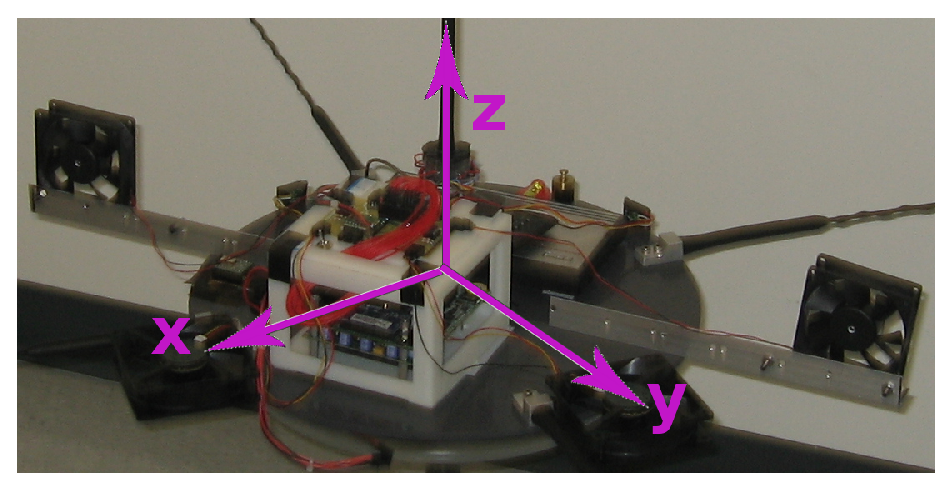
\psfig{file=figures/tsat_body_axes.eps,height=3in}}
  \caption{NASA MMS TableSat 1A Body Axes}
  \label{fig:TableSatBodyAxes}
\end{figure}
Table \ref{tbl:ActuatorConfiguration} shows the fan configuration for the NASA MMS TableSat 1A as arranged in Figure \ref{fig:TSatThrusters}.
\begin{table}[H]
  \centering
  \begin{tabular}{c|c|c|c|c}
    Fan & Center $\bs{f_c}$ (m) & Direction $\bs{n}$ & $F$ (N) & Max Moment $\frac{F \bs{n} \times \bs{f_c}}{|\bs{n}|}$ (Nm) \\ \hline
    1 & $(0.2474, -0.2474, 0)$ & $(-1, -1, 0)$ & 0.08 & $(0, 0, 0.039598)$ \\
    2 & $(-0.2474, 0.2474, 0)$ & $(-1, -1, 0)$ & 0.08 & $(0, 0, -0.039598)$ \\
    3 & $(0.25, 0, 0)$ & $(0, 0, -1)$ & 0.08 & $(0.02, 0, 0)$ \\
    4 & $(0, 0.25, 0)$ & $(0, 0, -1)$ & 0.08 & $(0, -0.02, 0)$ \\
  \end{tabular}
  \caption{Actuator configuration}
  \label{tbl:ActuatorConfiguration}
\end{table}
The code snippet below demonstrates the actuator module's functionality as it has been implemented in the TSatPy software.  Lines 4-13 define the geometry of the actuators displayed in Figure \ref{fig:TSatThrusters} with the addition of a hypothetical fifth actuator along with their center, direction of thrust, and maximum thrust force.

\begin{singlespace}
  \begin{minted}[mathescape,linenos,numbersep=10pt,frame=lines,framesep=2mm]{python}
import numpy as np
from TSatPy.Actuator import Actuator

configs = [{'type': 'fan', 'args': {'name': 'CW',
  'center': (0.2474, -0.2474, 0), 'direction': (-1, -1, 0), 'F': 0.08}
},{'type': 'fan', 'args': {'name': 'CCW1',
  'center': (-0.2474, 0.2474, 0), 'direction': (-1, -1, 0), 'F': 0.08}
},{'type': 'fan', 'args': {'name': 'CCW2',
  'center': (-0.2474, -0.2474, 0), 'direction': (1, -1, 0), 'F': 0.08}
},{'type': 'fan', 'args': {'name': 'NY', 'center': (0.25, 0, 0),
  'direction': (0, 0, 1), 'F': 0.08}
},{'type': 'fan', 'args': {'name': 'NX', 'center': (0, 0.25, 0),
  'direction': (0, 0, 1), 'F': 0.08}}]

def set_level(act, power_level):
    print 'Setting power level=%g for: %s' % (power_level, act)

def setup_actuators(configs):
    act = Actuator()
    for config in configs:
        act.add(config['type'], set_level, config['args'])
    return act

act = setup_actuators(configs)
print(act)
M = np.mat([0.03, 0.11, 0.04]).T
print("Request moment: %s" % (M.T))
print("Applied moment: %s" % (act.request_moment(M).T))

# Prints Out
# Actuator
#  <Fan CW moment=(0, -0, -0.0279901)>
#  <Fan CCW1 moment=(0, 0, 0.0279901)>
#  <Fan CCW2 moment=(0, 0, 0.0279901)>
#  <Fan NY moment=(0, -0.02, 0)>
#  <Fan NX moment=(0.02, 0, 0)>
# Request moment: [[ 0.03  0.11  0.04]]
# Setting power level=1 for: <Fan NX moment=(0.02, 0, 0)>
# Setting power level=0.714538 for: <Fan CCW1 moment=(0, 0, 0.0279901)>
# Setting power level=0.714538 for: <Fan CCW2 moment=(0, 0, 0.0279901)>
# Applied moment: [[ 0.02  0.    0.04]]
  \end{minted}
\nocite{minted}
\end{singlespace}

At line 24, the actuator instance is created and each fan's potential contribution to the overall control moment is calculated with
\begin{equation}
  \bs{M} = \frac{F \bs{n} \times \bs{f_c}}{|\bs{n}|}
\end{equation}
The script output shown above describes how a requested moment of $M_x = 0.03Nm, M_y = 0.11Nm, M_z = 0.04Nm$ would be applied to the five fan configuration.  The ``Nx'' fan can only produce a $0.02Nm$ moment, so gets set to full power to supply part of the requested $M_x = 0.03Nm$.  The ``Ny'' fan does not contribute since it's thrust is in the opposite direction from the needed $M_y = 0.11Nm$.  The ``CCW1'' and ``CCW2'' fans can not individually meet the requested $M_z = 0.04Nm$, but are able to collaboratively reach the requested moment by contributing 71\% each.  In the end, the actual moment that would be applied to the s/c is $M_x = 0.02Nm, M_y = 0Nm, M_z = 0.04Nm$.  This actual moment is both converted to voltages to be transmitted to the TableSat and supplied to the feedback loop to update the estimator's state propagation.

\section{Rate Control}
\label{sec:RateControl}

The first of the three controls goals introduced at the start of this chapter, is to attain a body rate of
\begin{equation}
  \bs{\omega}_d = 0 \bs{i} + 0 \bs{j} + 0.314 \bs{k}
\end{equation}
This desired rate is used for the tests in Sections \ref{subsec:PRateControl} through \ref{subsec:SlidingModeController}.  As explained at the start of the chapter, the following iterations of body rate controllers are tested under the assumption of perfect measurements to ensure appropriate functionality before combining with other modules for observer-based controls.
\subsection{P Rate Controller}
\label{subsec:PRateControl}
The initial controller tested is the proportional body rate controller of the form
\begin{equation}
  \bs{M}_{\omega} = \bs{K}_{\omega p} \left( \bs{\hat{\omega}} - \bs{\omega}_d \right)
  \label{eqn:PRateControl}
\end{equation}
Through a series of simulations with randomized initial conditions for body rates a gradient descent based on minimizing control effort is used to tune the proportional gains to
\begin{equation}
  \bs{K}_{\omega p} = \begin{bmatrix} 0.404 & 0 & 0 \\ 0 & 0.463 & 0 \\ 0 & 0 & 0.428 \end{bmatrix}
\end{equation}
Figure \ref{fig:PRateControl} graphs the body rates and applied moments for one of the the optimized gain tests.  The results show an adequate level of control that damps out the $\omega_x$ and $\omega_y$ rotations and maintains the 0.314 rad/sec for $\omega_z$.  Section \ref{subsec:PIDRateControl} expands on the controller to demonstrate the implementation of the integral and derivative components of the PID since the P-controller is susceptible to errors caused by noisy measurements.
\begin{figure}[H]
  \centerline{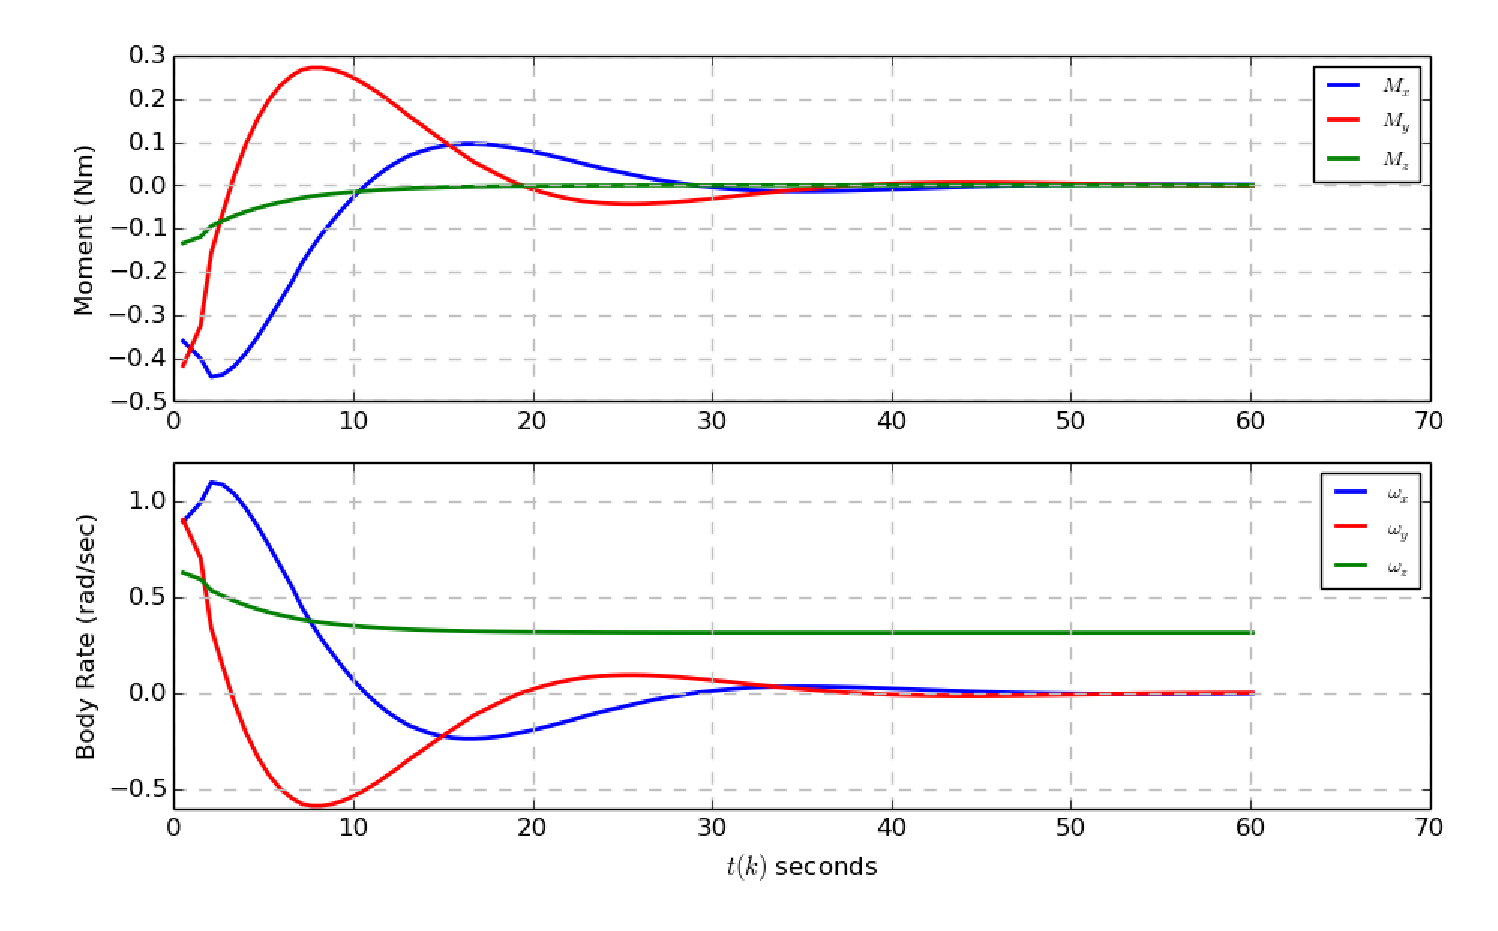
\psfig{file=figures/p_rate_control.eps,width=6in}}
  \caption{P rate control}
  \label{fig:PRateControl}
\end{figure}

\subsection{PID Rate Controller}
\label{subsec:PIDRateControl}

Expanding the proportional controller to include the integral and derivative term as shown in Equation \ref{eqn:PIDRateControl} can improve the performance slightly in the perfect measurement tests, but more importantly provides tools for dealing with noisy measurements when assessing observer-based controllers in Chapter \ref{chap:ObserverBasedControls}.  The integral and derivative terms are implemented with the $\Delta t_k$ adaptive step as with the PID estimator to help account for inconsistencies in update intervals by tracking the step size at each update.
\begin{equation}
  \begin{aligned}
    \bs{M}_{\omega} &= \bs{K}_{\omega p} \bs{\omega}_e + \bs{K}_{\omega i} \cdot (\Delta t_k \bs{I})\cdot \bs{\omega}_e + \bs{K}_{\omega d} \cdot \left(\frac{1}{\Delta t_k} \bs{I}\right) \cdot \bs{\omega}_e
  \end{aligned}
  \label{eqn:PIDRateControl}
\end{equation}
\begin{figure}[H]
  \centerline{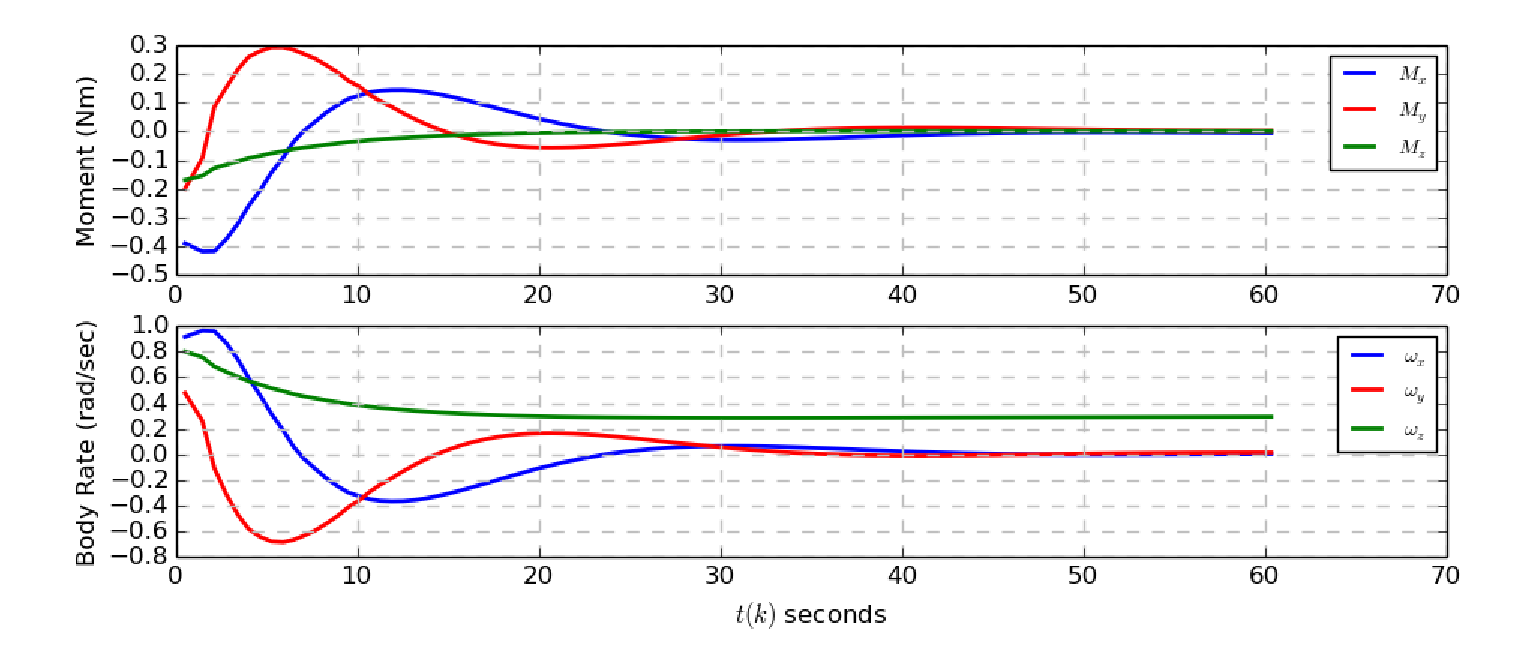
\psfig{file=figures/pid_rate_control.eps,width=6in}}
  \caption{PID rate control}
  \label{fig:PIDRateControl}
\end{figure}
The response curve in Figure \ref{fig:PIDRateControl} is generated from a random initial condition, and with the PID gains (Equation \ref{eqn:PIDRateControlGains}) tuned through gradient descent iterations based on minimizing the total control effort.  In the case of the perfect measurements, the addition correction two control terms generally reduce the overshoot of the response, but do not significantly shorten the time to bring the system to a steady state.
\begin{equation}
  \begin{aligned}
    \bs{K}_{\omega p} &= \begin{bmatrix} 0.424 & 0 & 0 \\ 0 & 0.416 & 0 \\ 0 & 0 & 0.346 \end{bmatrix},
    \bs{K}_{\omega i} = \begin{bmatrix} 0.006 & 0 & 0 \\ 0 & 0.003 & 0 \\ 0 & 0 & 0.005 \end{bmatrix} \\
    \bs{K}_{\omega d} &= \begin{bmatrix} 0.044 & 0 & 0 \\ 0 & 0.072 & 0 \\ 0 & 0 & 0.042 \end{bmatrix}
  \end{aligned}
  \label{eqn:PIDRateControlGains}
\end{equation}
Figure \ref{fig:PIDRateControlMoments} shows how the moments from each of the PID components contributes to the overall moments applied.  The addition of the derivative term gives the system a slightly quicker response that just the P-controller, and in this perfect measurement scenario the the overall performance of the system would benefit from the integral term being removed altogether since it doesn't contribute much to the initial response and even causes a larger steady state error than the P-controller.
\begin{figure}[H]
  \centerline{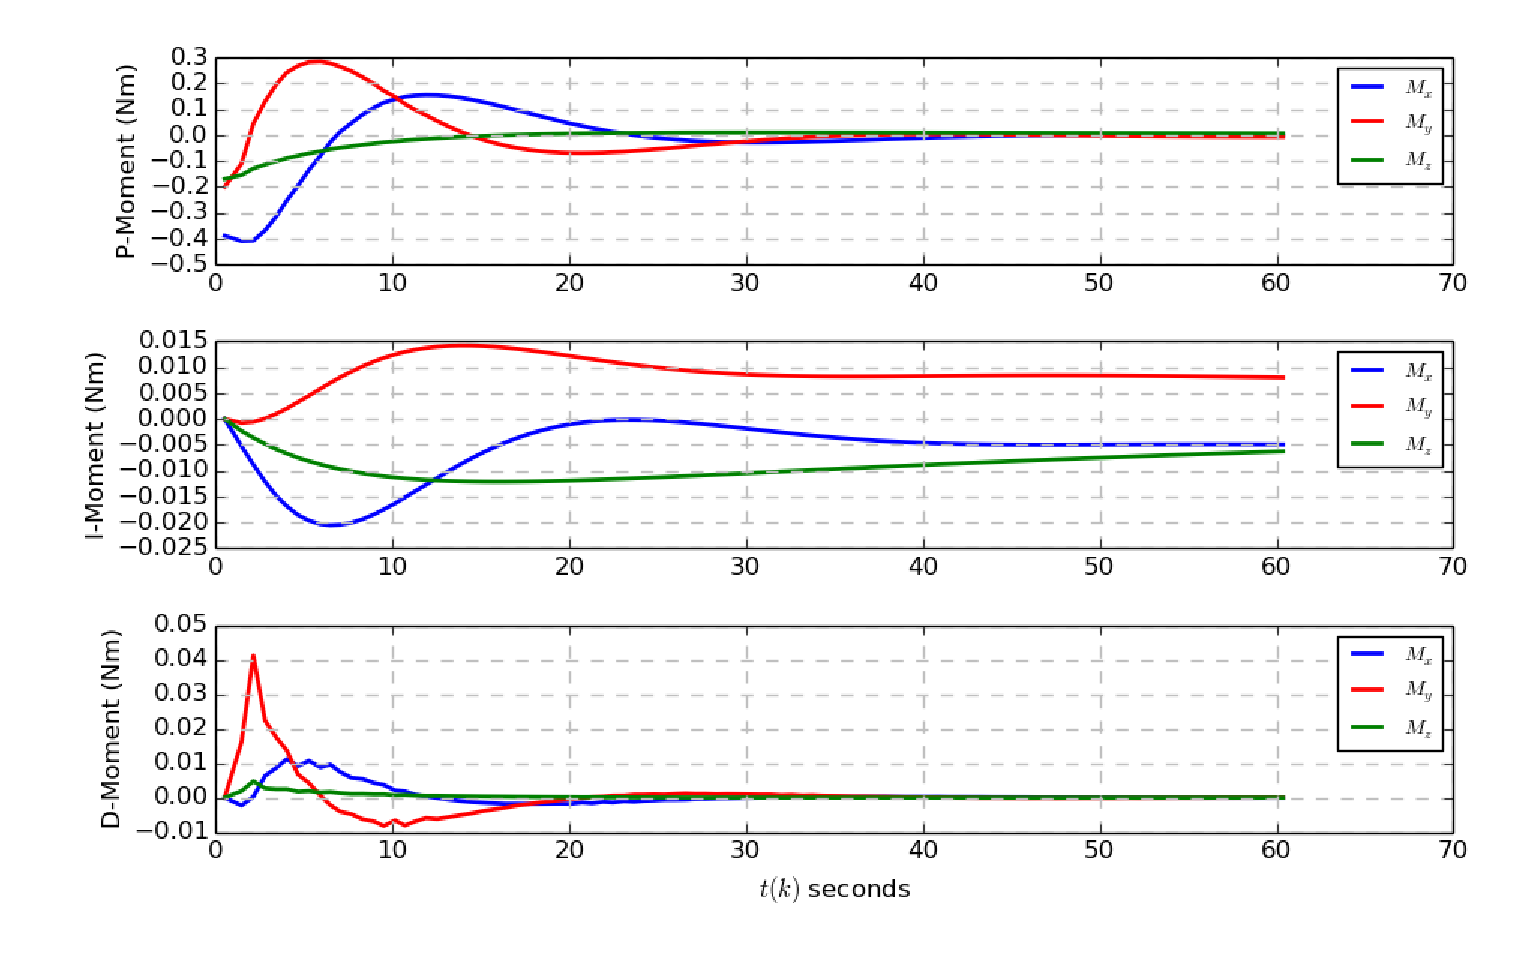
\psfig{file=figures/pid_rate_control_moments.eps,width=6in}}
  \caption{PID rate control moments}
  \label{fig:PIDRateControlMoments}
\end{figure}

\subsection{Sliding Mode Controller}
\label{subsec:SlidingModeController}

The Sliding Mode Controller (SMC) operates similarly to a proportional controller and is governed by the equation
\begin{equation}
  \bs{M}_{\omega} = \bs{L}_{\omega} \bs{\omega}_e + \bs{K}_{\omega}\bs{1}_s \big(\bs{\omega}_e \big)
  \label{eqn:SMController}
\end{equation}
where $\bs{L}_{\omega}$ is the proportional gain and the $\bs{1}_s$ function can take a number of forms such as the signum and arctangent function.  In this thesis, the smc uses the saturation function such that $\bs{1}_s$ is
\begin{equation}
  \bs{1}_s \big(\bs{\omega}_e \big) = sat \begin{bmatrix} \omega_{ex} / S_{\omega} &0 &0 \\ 0 & \omega_{ey} / S_{\omega} & 0 \\ 0 & 0 & \omega_{ez} / S_{\omega} \end{bmatrix}
\end{equation}
The response to the test configuration shows significant improvements in performance over the P and PID rate controller as shown if Figure \ref{fig:SMCRateControl}.
\begin{figure}[H]
  \centerline{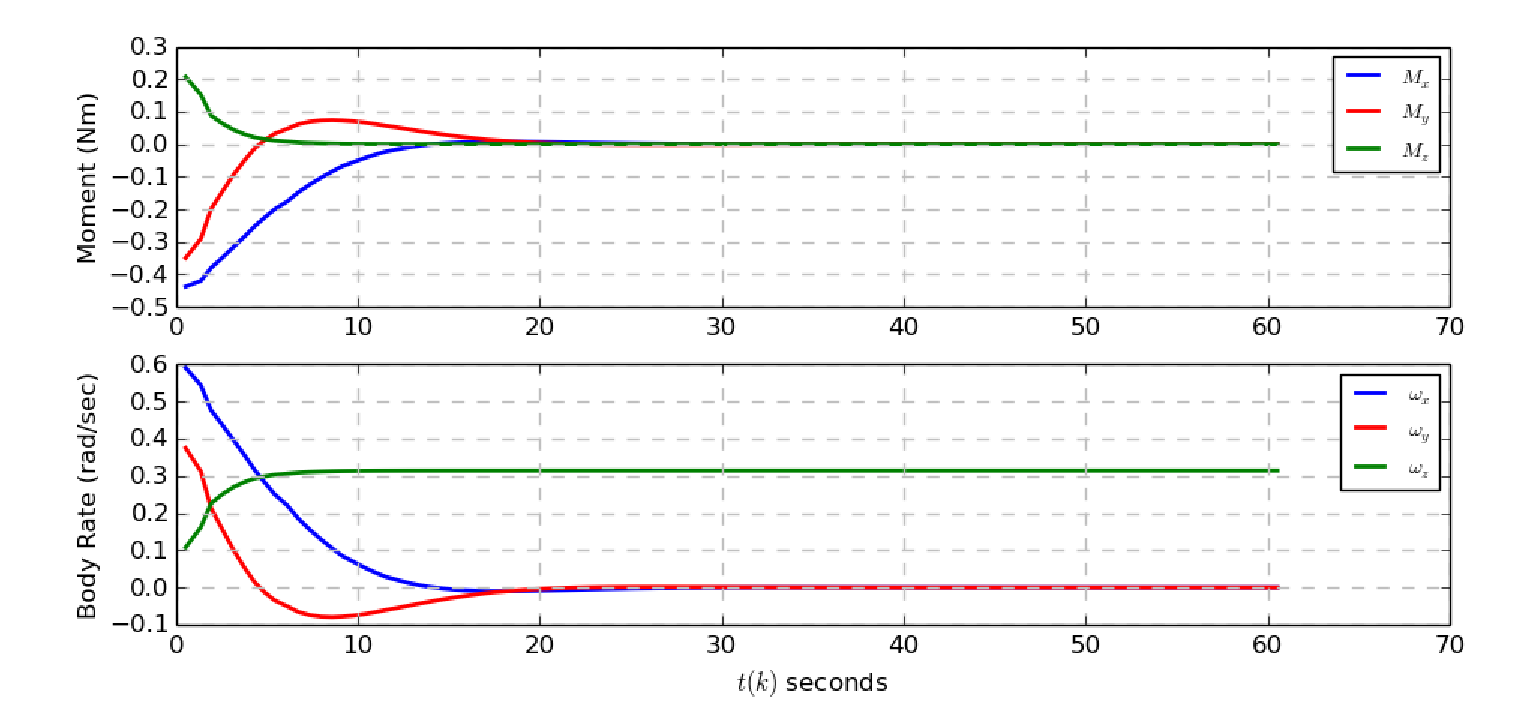
\psfig{file=figures/smc_rate_control.eps,width=6in}}
  \caption{SMC rate control}
  \label{fig:SMCRateControl}
\end{figure}
Breaking the overall moment values into the separate term's contributions (Figure \ref{fig:SMCRateControlMoments}) shows the similar profile between the proportional and saturation term contributions with the exception of the peaks missing from the saturation response.
\begin{figure}[H]
  \centerline{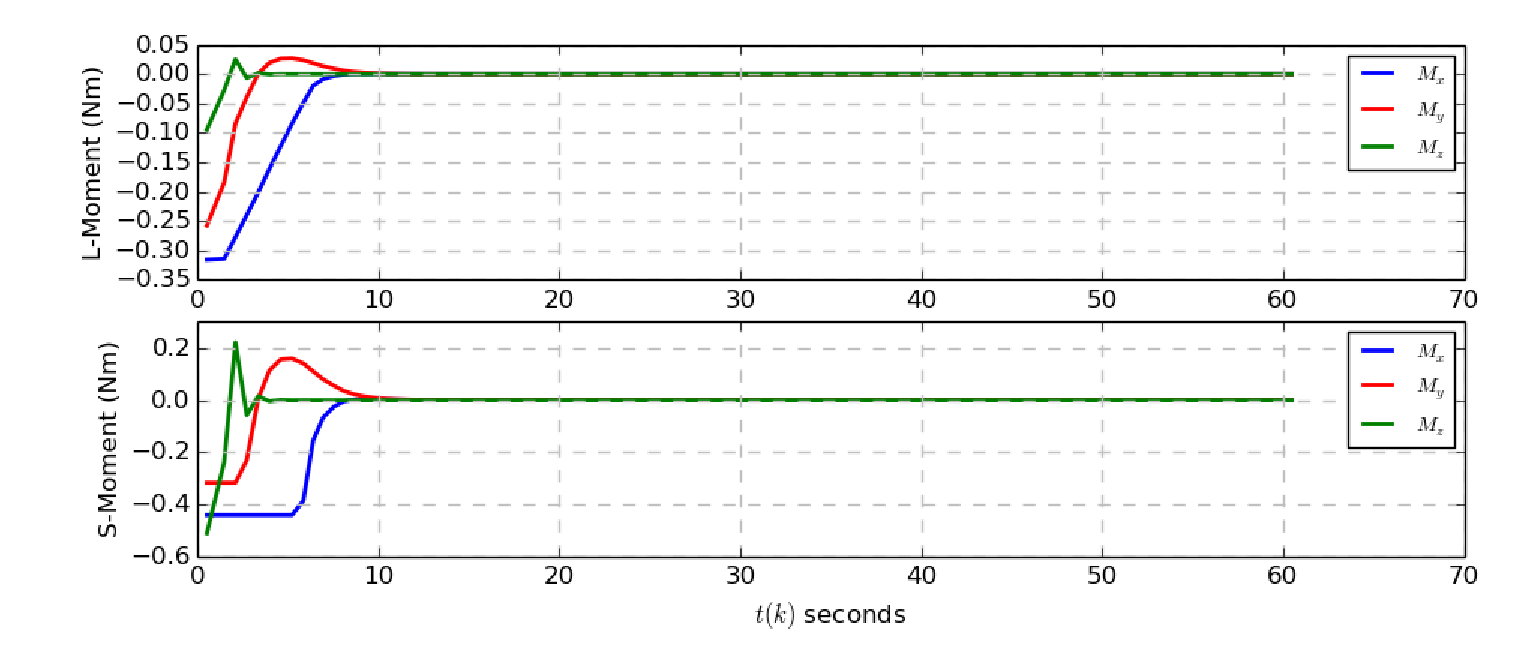
\psfig{file=figures/smc_rate_control_moments.eps,width=6in}}
  \caption{SMC rate control moments}
  \label{fig:SMCRateControlMoments}
\end{figure}
The SMC response in Figures \ref{fig:SMCRateControl} and \ref{fig:SMCRateControlMoments}, is generated with the following gain values tuned through a gradient descent search that minimizes control effort.
\begin{equation}
    \bs{L}_{\omega} = \begin{bmatrix} 0.3983 & 0 & 0 \\ 0 & 0.3828 & 0 \\ 0 & 0 & 0.4160 \end{bmatrix},
    \bs{K}_{\omega} = \begin{bmatrix} 0.4399 & 0 & 0 \\ 0 & 0.5097 & 0 \\ 0 & 0 & 0.3162 \end{bmatrix},
    S_{\omega} = 0.1404
  \label{SMCRateControlGains}
\end{equation}
With the perfect measurements in this test, the saturation term adds a significant performance improvement over the P and PID implementations.  Additionally, with two fewer gain values tuning the SMC is slightly less involved than the PID body rate controller.

\section{Quaternion to Moment Conversion}
\label{sec:QuaternionToMomentConversion}

The remainder of this chapter focuses on the attitude control problem to correct for nutation (Section \ref{sec:AttitudeAndNutationControl}) and the integration of the attitude and rate controller (Section \ref{sec:AttitudeandBodyRateControl}).  The proper conversion from an attitude error measurement to actuator moments is critical to providing a robust control method.

The attitude error measurement is calculated through the quaternion multiplicative method as is established in Section \ref{sec:HighIntegrityStateAdjustments}

\begin{equation}
  \bs{q}_e = \bs{q}_d^* \otimes \bs{\hat{q}}
\end{equation}

Unlike with the estimator where the input and output formats are both quaternions, the quaternion error in the controller $\bs{q}_e$ is composed of four parameters that need to map to three moments values.  The commonly used method for this is to fall back on matrix algebra where

\begin{equation}
  \bs{M}_q = \begin{bmatrix} 3 \times 4 \end{bmatrix} \begin{bmatrix} q_1 & q_2 & q_3 & q_0 \end{bmatrix}^T
  \label{eqn:traditional_attitude_controller}
\end{equation}

There are two main issues with this approach.  First is that the quaternion parameters are sinusoidal in nature, such that the conversion to moment values through the matrix multiplication, the magnitude of the moment do not scale linearly with the magnitude of the attitude error.

The second issue is that the quaternion is comprised of a vector and scalar that provide two separate types of information about the attitude error.  Lumping the two together in a single matrix multiplication ignores the physical representation of their values.  The vector defines the Euler axis which gives the attitude error it's direction.  A vector component with $q_1 = q_3 = 0, q_2 \ne 0$ means that to move the estimated satellite attitude to the desired attitude requires a rotation about just the body-fixed $y$-axis which requires a moment couple in just $M_y$.  This can be represented simply as
\begin{equation}
  \bs{M}_{q} = \bs{v}_e
\end{equation}
This provides a basis for the direction of the moment couple, but since the rotational quaternion is fixed at a unit norm, the magnitude of the vector component varies with the size of the error.  This is compensated for by normalizing the vector.
\begin{equation}
  \bs{M}_{q} = \bs{\hat{e}}_e
  \label{eqn:quat_vector_to_moment}
\end{equation}
With Equation \ref{eqn:quat_vector_to_moment} establishing the direction for the actuator moments, the remaining issue is to determine how to scale the moment couples in relation to the size of the error.  The remaining $q_0$ quantity is a reasonable first choice as
\begin{equation}
  \bs{M}_{q} = kq_{0e} \bs{\hat{e}}_e
\end{equation}
$q_{0e}$, as with the vector, is a sinusoidal measure.  The underlying $\theta$ measure of the quaternion rotation however is a direct measure of the attitude error.  Extracting the $\theta$ measure from $q_{0e}$ and incorporating into the moment calculation yields
\begin{equation}
  \bs{M}_{q} = \left[- k \cos^{-1} (q_{0e}) \right] \bs{\hat{e}}_e
  \label{eqn:QuaternionToMomentConversion}
\end{equation}
This conversion is used throughout all attitude control calculations in the remainder of this chapter and in the observer-based controllers in Chapter \ref{chap:ObserverBasedControls}.










\section{Attitude and Nutation Control}
\label{sec:AttitudeAndNutationControl}

Section \ref{sec:RateControl} covered the design of the rate controller which addresses the first controller goal to maintain a spin rate of $\omega_z = 3$ rpm.  This section ignores the rate control requirement and focuses strictly on the attitude control problem by incorporating the quaternion to moment conversion in Equation \ref{eqn:QuaternionToMomentConversion} into a PID and SMC attitude controller.   Later, section \ref{sec:AttitudeandBodyRateControl} combines the attitude and body rate controls into a single controller.

\subsection{P Attitude Control}
\label{subsec:PAttitudeControl}

Starting with a simplest design of the proportional attitude control, equation \ref{eqn:QuaternionToMomentConversion} can be directly applied as
\begin{equation}
  \bs{M}_{q} = \left[- K_{qp} \cos^{-1} \big(q_{0e} \big) \right] \bs{\hat{e}}_e \\
  \label{eqn:PAttitudeControl}
\end{equation}
This format of the proportional controller provides a significant time savings over the common method in Equation \ref{eqn:traditional_attitude_controller} when optimizing gains since instead of 12 gain values to tune, the controller is limited to a single gain.

To assess the accurate implementation, a the system is initialized to a state of
\begin{equation}
  \bs{x}_0 = \begin{bmatrix} 0 \bs{i} -0.0477 \bs{j} -0.477 \bs{k} +0.8778 \\ 0 \bs{i} -0.01 \bs{j} +0.2 \bs{k} \end{bmatrix}
\end{equation}
which is essentially a 1 radian twist about the $z$-axis with a slight push out of the spin plane with the initial $\omega_y = -0.01$ rad/sec.  The controller is set with a desired state to return the satellite back to the standard attitude where the body-fixed reference frame is aligned with the global reference frame
\begin{equation}
  \bs{q}_d = 0 \bs{i} +0 \bs{j} +0 \bs{k} + 1
\end{equation}
and a chosen proportional gain of
\begin{equation}
  K_{qp} = 0.04
\end{equation}
The results from the test are shown in Figure \ref{fig:PAttitudeControl}.  The simulation ran for 120 seconds.  The top graph displays the calculated moments required to compensate for the attitude error.  As expected, the $M_z$ is shows the P-controller spring like oscillating moments as the satellite twists back and forth.  The center graph displays the $\theta$ measure that quantifies the distance between the current and desired attitude.  With this measure, it's visible that while the majority of the attitude error is linked to the twist about the $z$-axis.  The error gets progressively larger through each rotation as some of the rotational motion gets transferred to the out of plane motion.
\begin{figure}[H]
  \centerline{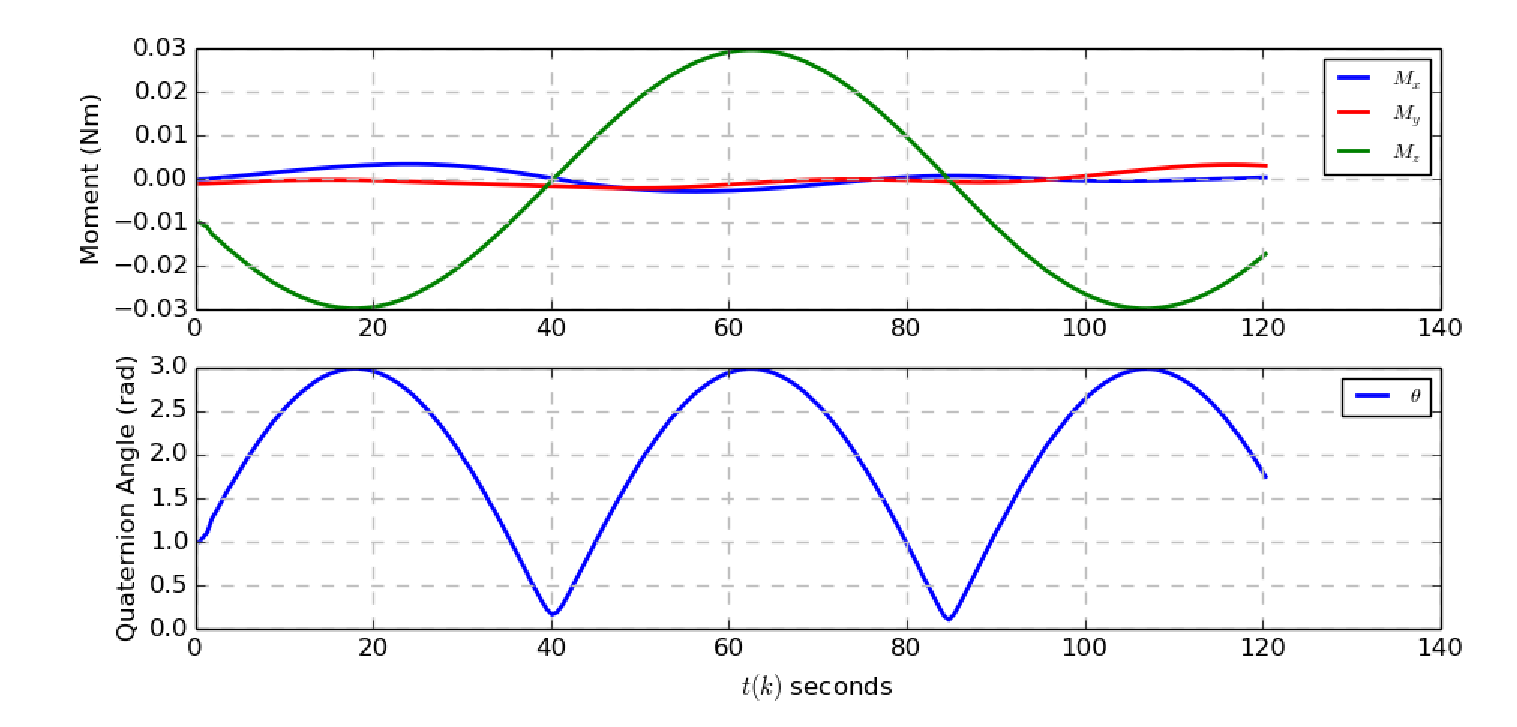
\psfig{file=figures/p_attitude_control.eps,width=6in}}
  \caption{P Attitude Control}
  \label{fig:PAttitudeControl}
\end{figure}








\subsection{Quaternion Decomposition for Nutation Control}
\label{subsec:QuaternionDecompositionForNutationControl}



Prior to combining the attitude control from Section \ref{subsec:PAttitudeControl} with the body rate control from Section \ref{sec:RateControl}, the controller needs to incorporate the quaternion decomposition method in Equation \ref{eqn:quaternion_decomposition_derivation}.  The advantage to incorporating this into a controller is being able to take the quaternion portion of the state error, decompose it into its associated rotation and nutation quaternions, and replace the quaternion error with the nutation quaternion error.  This limits the attitude controller to just worry about correcting for nutation regardless of the rotational position or angular velocity.

The proportional attitude control from Equation \ref{eqn:PAttitudeControl} becomes
\begin{equation}
  \bs{M}_{q} = \left[- K_{qp} \cos^{-1} \big(q_{0en} \big) \right] \bs{\hat{e}}_{en} \\
\end{equation}
where $q_{0en}$ is the scalar component of the error quaternion's nutation component, and $\bs{\hat{e}}_{en}$ is the normalized Euler axis for the nutation component.

The following code snippet shows how the incorporation of this method in the TSatPy software where the state error $x_e$ has its attitude measure adjusted to represent only the nutation error.

\begin{singlespace}
  \begin{minted}[mathescape,linenos,numbersep=10pt,frame=lines,framesep=2mm]{python}
from TSatPy.State import State, Quaternion, BodyRate

print("State Error")
x_e = State(
    Quaternion([0,0.1,1],radians=1),
    BodyRate([0,-0.01,0.2]))
print("x_e: %s" % (x_e))

print("Decomposed Quaternion")
q_r, q_n = x_e.q.decompose()
print("q_r: %s" % q_r)
print("q_n: %s" % q_n)

print("Nutation Only State Error")
x_e.q = q_n
print("x_e: %s" % (x_e))

# Prints Out
# State Error
# x_e: <Quaternion [-0 -0.0477046 -0.477046], 0.877583>,
#      <BodyRate [0 -0.01 0.2]>
# Decomposed Quaternion
# q_r: <Quaternion [0 0 -0.47759], 0.878583>
# q_n: <Quaternion [-0.0227833 -0.0419125 -0], -0.998861>
# Nutation Only State Error
# x_e: <Quaternion [-0.0227833 -0.0419125 -0], -0.998861>,
#      <BodyRate [0 -0.01 0.2]>
  \end{minted}
\nocite{minted}
\end{singlespace}

Now that there is a defined method for separating the allowed rotation from the unwanted nutation, Section \ref{subsec:PNutationControl} shows the decomposition in use with the proportional attitude controller.

\subsection{P Nutation Control}
\label{subsec:PNutationControl}

Using the proportional control
\begin{equation}
  \bs{M}_{q} = \left[- K_{qp} \cos^{-1} (q_{0n}) \right] \bs{\hat{e}}_n
  \label{eqn:PNutationControl}
\end{equation}
with the same initial state and desired quaternion as the proportional attitude controller
\begin{equation}
  \bs{x}_0 = \begin{bmatrix} 0 \bs{i} -0.0477 \bs{j} -0.477 \bs{k} +0.8778 \\ 0 \bs{i} -0.01 \bs{j} +0.2 \bs{k} \end{bmatrix}
\end{equation}
\begin{equation}
  \bs{q}_d = 0 \bs{i} +0 \bs{j} +0 \bs{k} + 1
\end{equation}
\begin{figure}[H]
  \centerline{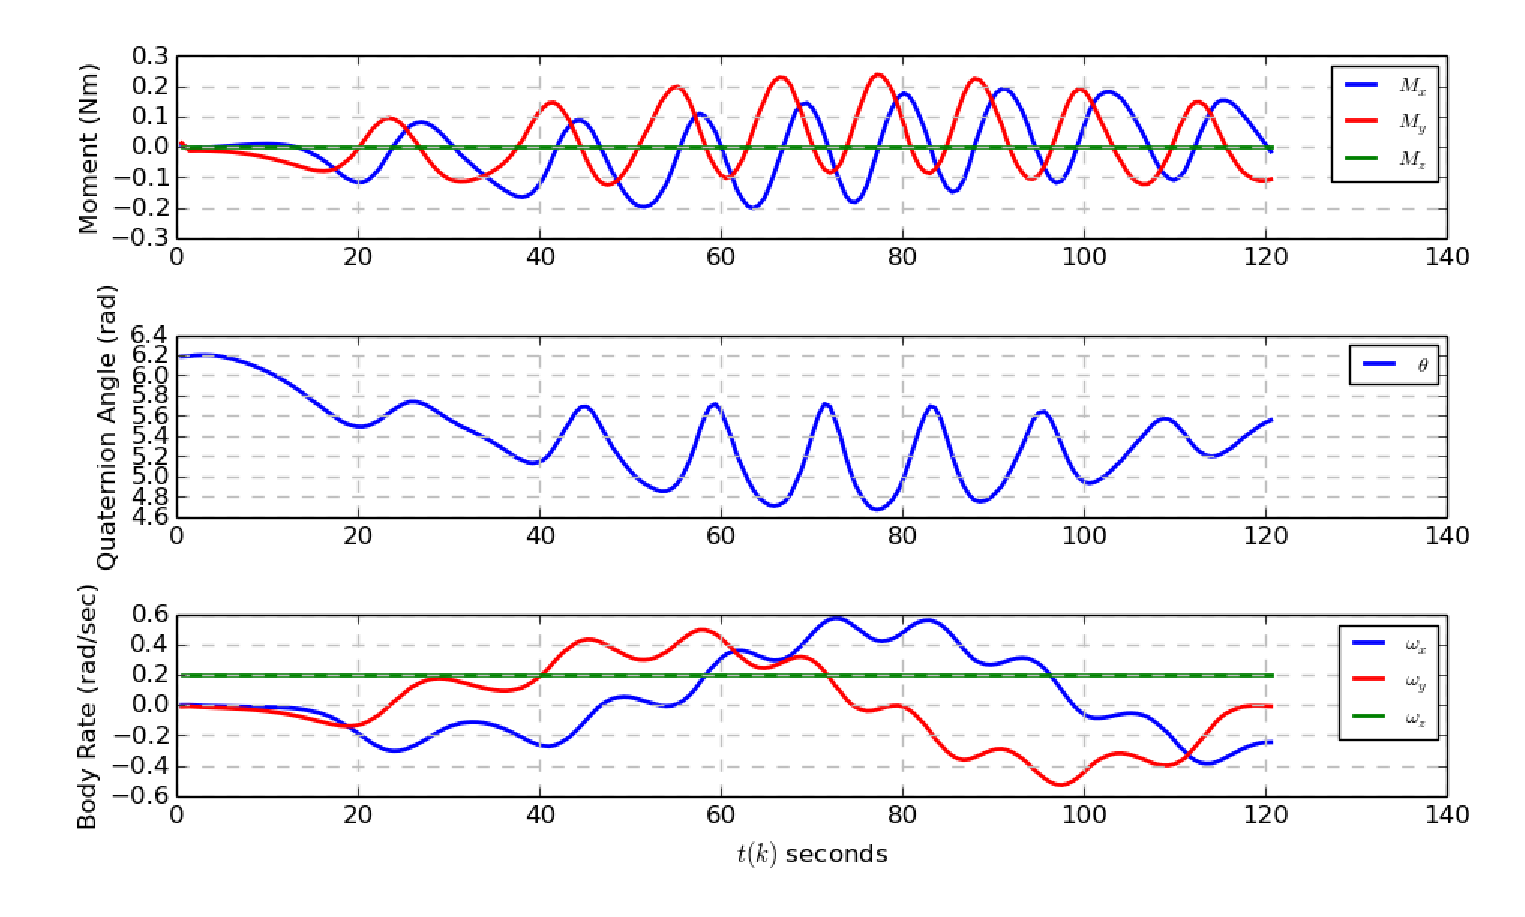
\psfig{file=figures/p_nutation_control.eps,width=6in}}
  \caption{P Nutation Control}
  \label{fig:PNutationControl}
\end{figure}
Figure \ref{fig:PNutationControl} shows the resulting control moments, quaternion angle error, and body rates.  In the first and last graphs, the body rates and moments show the expected behavior where the corrections for initial nutation are causing fluctuations in the $\omega_x$ and $\omega_z$ body rates, but the $\omega_z$ body remains unchanged.  This means that for spin-stabilized systems like NASA's MMS mission satellite, the controller can correct for nutation errors unaffected by the constant spin rate.  The same can be seen in the first graph where moments are applied about the $x$ and $y$ axes, but no attempt is made to control for the initial spin about $z$.
The center plot tracking quaternion angle, shows that while some of the nutation is removed the proportional nutation controller is clearly not enough to remove all nutation.


\section{Attitude and Body Rate Control}
\label{sec:AttitudeandBodyRateControl}

Sections \ref{sec:RateControl} and \ref{sec:AttitudeAndNutationControl} have established methods to address the spin rate and nutation control goals.  In this section the two are used together.  In Section \ref{subsec:FixedAttitudeControl}, the attitude and body rate controllers are combined to take a satellite from an initialized uncontrolled spin and bring it to the standard orientation with fixed-body axes aligned with the global axes.  Section \ref{subsec:SpinStabilizedControl} follows up by releasing the restriction on motion about the $z$ axis and takes the satellite's initial uncontrolled spin to a nutation-free rotation about the $z$-axis.
\begin{equation}
    \bs{M} = \bs{M}_{q} + \bs{M}_{\omega}
\end{equation}
For consistency, all tests in this section are initialized with the following state
\begin{equation}
  \bs{x}_0 = \begin{bmatrix} -0.532 \bs{i} -0.417 \bs{j} -0.275 \bs{k} +0.684 \\ 0.315 \bs{i} +0.207 \bs{j} +0.113 \bs{k} \end{bmatrix}
  \label{eqn:attitude_and_body_rate_control_ic}
\end{equation}

\subsection{Fixed Attitude Control}
\label{subsec:FixedAttitudeControl}
The PID controllers are defined as
\begin{equation}
  \begin{aligned}
    \bs{M} &= \bs{M}_{q} + \bs{M}_{\omega} \\
    \bs{M}_{q} &= \left[- K_{qp} \cos^{-1} (q_{0e}) \right] \bs{\hat{e}}_e + \left[- K_{qi} \cos^{-1} (q_{0ei}) \right] \bs{\hat{e}}_{ei} + \left[- K_{qd} \cos^{-1} (q_{0ed}) \right] \bs{\hat{e}}_{ed} \\
    \bs{M}_{\omega} &= \bs{K}_{\omega p} \bs{\omega}_e + \bs{K}_{\omega i} \cdot (\Delta t_k \bs{I})\cdot \bs{\omega}_e + \bs{K}_{\omega d} \cdot \left(\frac{1}{\Delta t_k} \bs{I}\right) \cdot \bs{\omega}_e
  \end{aligned}
\end{equation}
where $\bs{\hat{e}}_e, \bs{\hat{e}}_{ei}, \bs{\hat{e}}_{ed}$ are the Euler axes for the quaternion error, quaternion error integral, and quaternion error derivative respectively with the integral $\bs{q}_{ei}$ and derivative $\bs{q}_{ed}$ quaternions from Equations \ref{eqn:IEstimator} and \ref{eqn:DEstimator}.

The results from the PID body rate and attitude controller are shown in Figures \ref{fig:PIDAttitudeAndRateControl} and \ref{fig:PIDAttitudeAndRateControlMoments} when tested with the following parameters
\begin{equation}
  \begin{aligned}
    K_{qp} &= 0.6022,K_{qi} = 0.04656,K_{qd} = 0.8554 \\
    K_{\omega p} &= \bs{I} \begin{bmatrix} 0.70326 & 0.7203 & 0.61757 \end{bmatrix}^T \\
    K_{\omega i} &= \bs{I} \begin{bmatrix} 0.04207 & 0.06999 & 0.018591 \end{bmatrix}^T \\
    K_{\omega d} &= \bs{I} \begin{bmatrix} 0.4096 & 0.6032 & 0.6123 \end{bmatrix}^T
  \end{aligned}
\end{equation}
\begin{figure}[H]
  \centerline{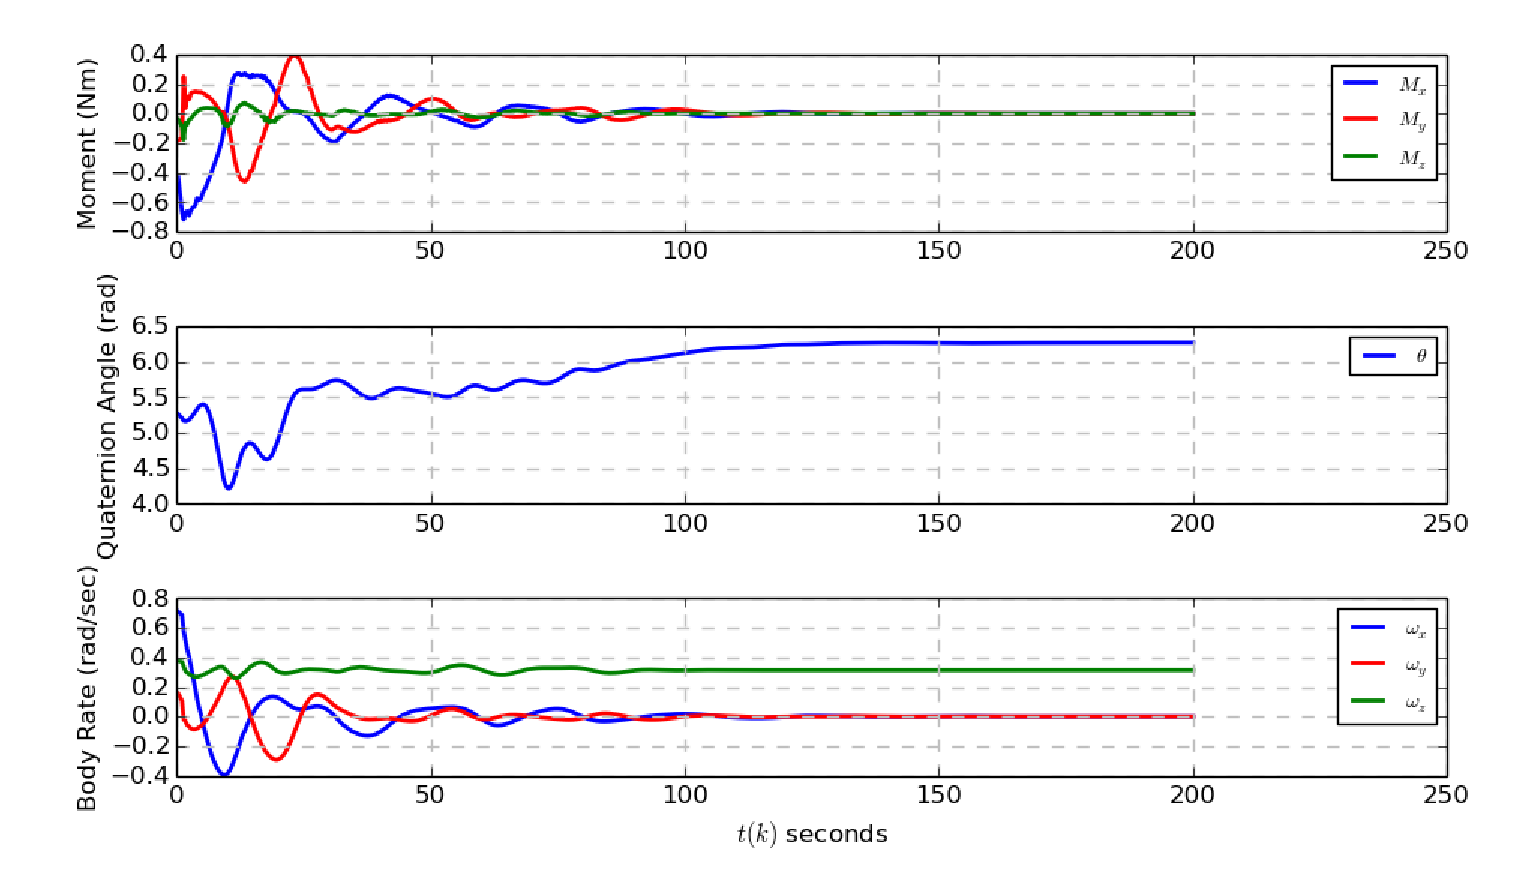
\psfig{file=figures/pid_attitude_and_rate_control.eps,width=6in}}
  \caption{PID Attitude and Rate Control}
  \label{fig:PIDAttitudeAndRateControl}
\end{figure}
Figure \ref{fig:PIDAttitudeAndRateControl} shows a significant improvement to the body rate response over previous body rate only tests.  All error and oscillations in the quaternion angle were also eliminated.  The graphs in \ref{fig:PIDAttitudeAndRateControlMoments} attribute the fast conversion to the desired attitude initially to the proportional and derivative components with the integral component eliminating the final steady state error.
\begin{figure}[H]
  \centerline{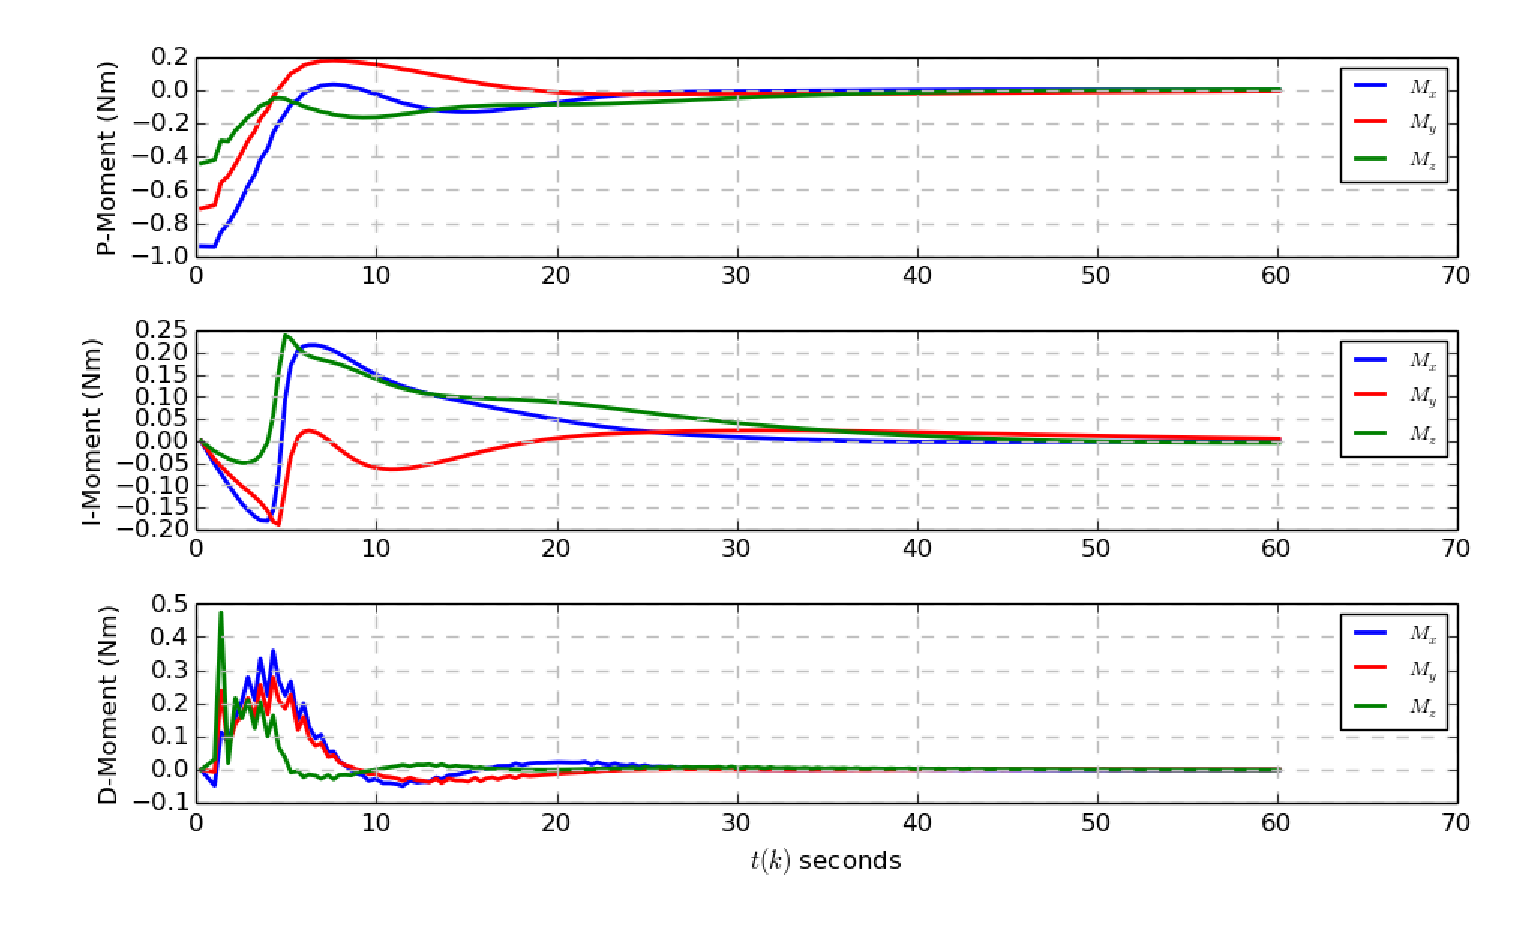
\psfig{file=figures/pid_attitude_and_rate_control_moments.eps,width=6in}}
  \caption{PID Attitude and Rate Control Moments}
  \label{fig:PIDAttitudeAndRateControlMoments}
\end{figure}

The Sliding Mode Controllers are defined as
\begin{equation}
  \begin{aligned}
    \bs{M} &= \bs{M}_{q} + \bs{M}_{\omega} \\
    \bs{M}_{q} &= \left[- L_{q} \cos^{-1} (q_{0e}) \right] \bs{\hat{e}}_e + \left[ K_{q} sat \left( \frac{-2\cos^{-1} (q_{0e})}{S_q} \right) \right] \bs{\hat{e}}_e \\
    \bs{M}_{\omega} &= \bs{L}_{\omega} \bs{\omega}_e + \bs{K}_{\omega}\bs{1}_s \big(\bs{\omega}_e / S_{\omega} \big) \\
    \bs{1}_s \big(\bs{\omega}_e / S_{\omega} \big) &= \begin{bmatrix} sat (\omega_{ex} / S_{\omega}) &0 &0 \\ 0 & sat (\omega_{ey} / S_{\omega}) & 0 \\ 0 & 0 & sat (\omega_{ez} / S_{\omega}) \end{bmatrix}
  \end{aligned}
  \label{eqn:sliding_mode_control}
\end{equation}
Figures \ref{fig:SMCAttitudeAndRateControl} and \ref{fig:SMCAttitudeAndRateControlMoments} show the response for the SMC to the attitude and body rate control test run.  Through a gradient descent search, the SMC parameters are tuned to
\begin{equation}
  \begin{aligned}
    L_q &= 0.408, \bs{L}_{\omega} = \bs{I} \begin{bmatrix} 0.708 & 0.678 & 0.525 \end{bmatrix}^T \\
    K_q &= 0.500, \bs{K}_{\omega} = \bs{I} \begin{bmatrix} 0.745 & 0.816 & 0.666 \end{bmatrix}^T \\
    S_q &= 0.607, S_{\omega} = 0.315
  \end{aligned}
\end{equation}
\begin{figure}[H]
  \centerline{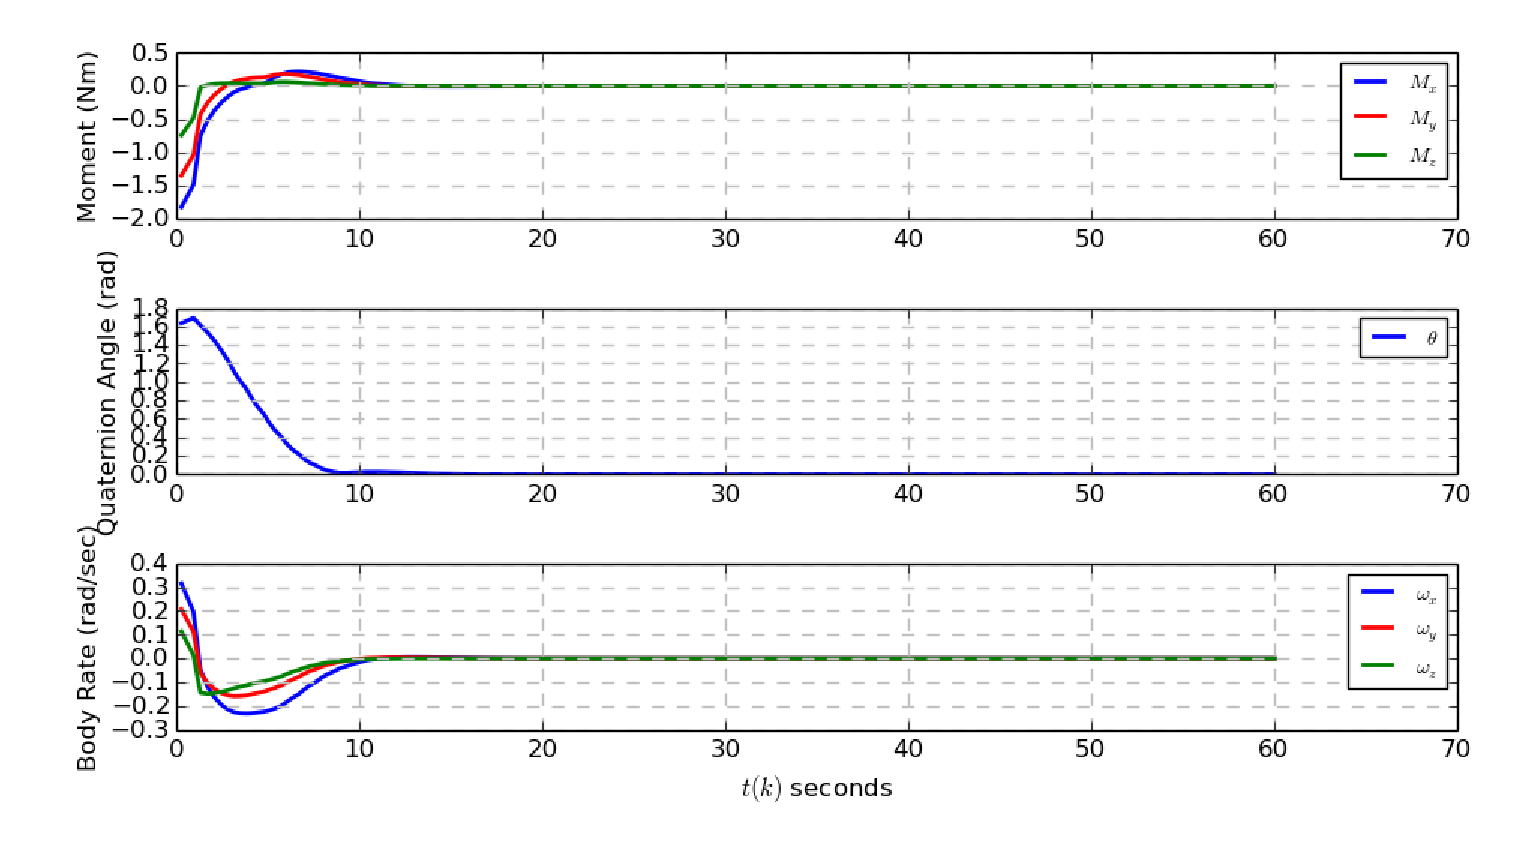
\psfig{file=figures/smc_attitude_and_rate_control.eps,width=6in}}
  \caption{SMC Attitude and Rate Control}
  \label{fig:SMCAttitudeAndRateControl}
\end{figure}
\begin{figure}[H]
  \centerline{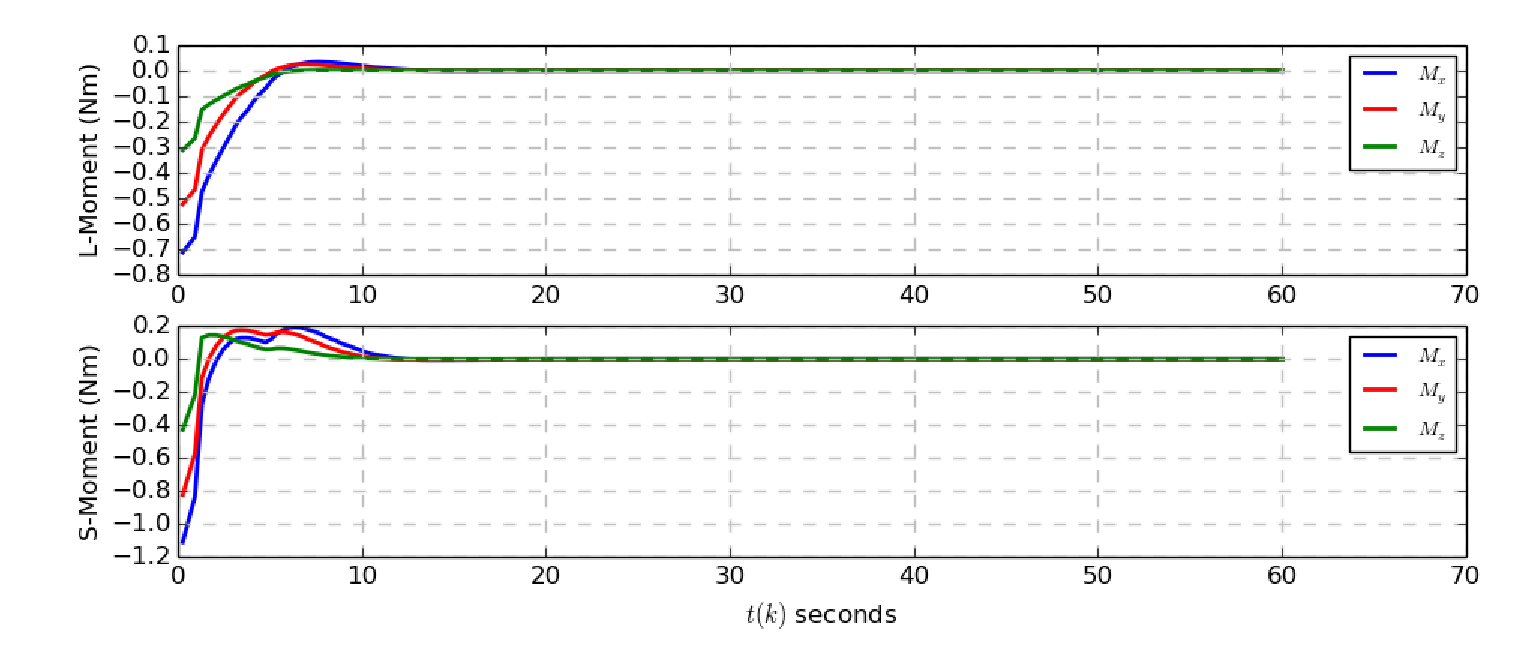
\psfig{file=figures/smc_attitude_and_rate_control_moments.eps,width=6in}}
  \caption{SMC Attitude and Rate Control Moments}
  \label{fig:SMCAttitudeAndRateControlMoments}
\end{figure}
As with the body rate comparative tests, the sliding mode controller shows a significant improvement in performance compared to the PID controller for the fixed attitude and body rate tests.  Section \ref{subsec:SpinStabilizedControl} follows up on these results by freeing up the motion about the $z$-axis for a spin-stabilized and nutation rejection test.

\subsection{Spin-Stabilized Control}
\label{subsec:SpinStabilizedControl}

This section verifies the ability for a controller to take the fixed attitude control problem from Section (\ref{subsec:FixedAttitudeControl}) and release the quaternion restriction on the rotational motion leaving the system to control five degrees of freedom $\omega_z = 0.314, \omega_x = \omega_y = 0$ and zero nutation about the $x$ and $y$ axes.  Since the Sliding Mode Controller has regularly out performed the PID controller, the spin-stabilized controller will run with control Equation (\ref{eqn:sliding_mode_control}) using the following parameters.
\begin{equation}
  \begin{aligned}
    L_q &= 0.01, \bs{L}_{\omega} = \bs{I} \begin{bmatrix} 0.398 & 0.383 & 0.416 \end{bmatrix}^T \\
    K_q &= 0.01, \bs{K}_{\omega} = \bs{I} \begin{bmatrix} 0.440 & 0.510 & 0.316 \end{bmatrix}^T \\
    S_q &= 0.01, S_{\omega} = 0.140
  \end{aligned}
\end{equation}

The initial convergence of to the spin stabilized state is rapid as in previous test configurations for the SMC.  In this case, the system remains with a steady state error.  Some manual gain tuning does not show any significant improvements and appears from the error measurements to be lagging behind the desired state and rocking back and forth about the desired spin axis.  Additional testing for gain tuning or improved visualizations such as the tPlot discussed in Section \ref{sec:ObjectOrientedNSSControlSystem} would help diagnose the source of the error.
\begin{figure}[H]
  \centerline{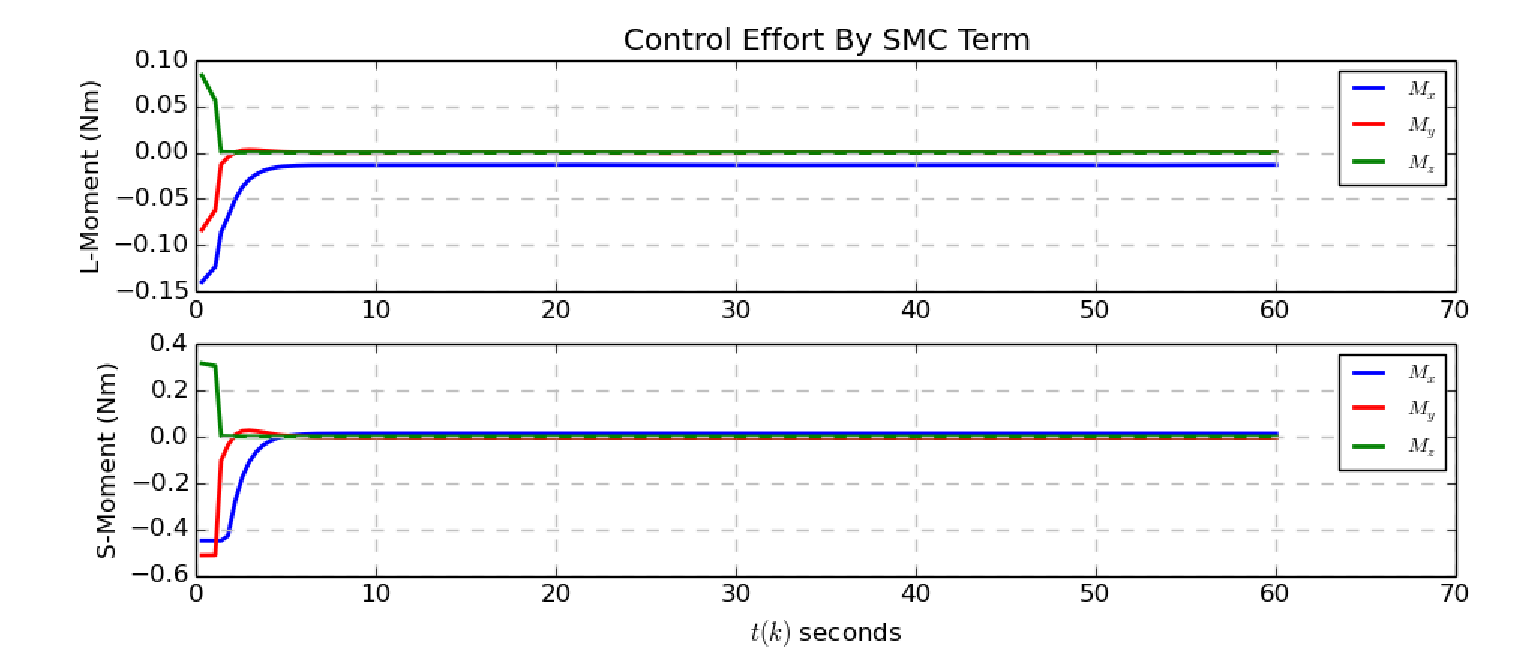
\psfig{file=figures/smc_nutation_and_rate_control.eps,width=6in}}
  \caption{SMC Nutation and Rate Control}
  \label{fig:SMCNutationAndRateControl}
\end{figure}
\begin{figure}[H]
  \centerline{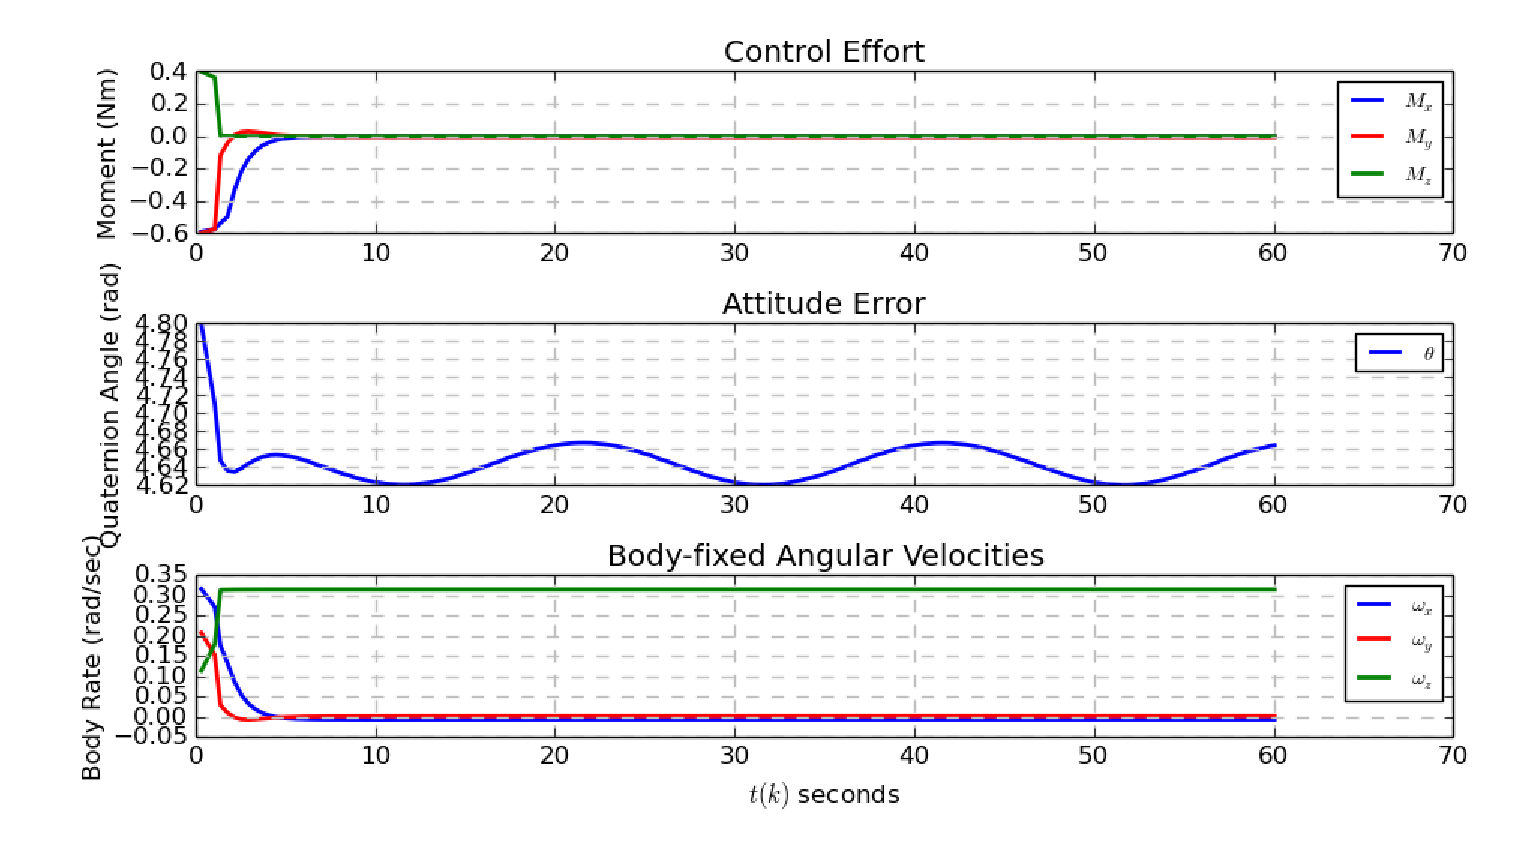
\psfig{file=figures/smc_nutation_and_rate_control_moments.eps,width=6in}}
  \caption{SMC Nutation and Rate Control Moments}
  \label{fig:SMCNutationAndRateControlMoments}
\end{figure}



\chapter{OBSERVER BASED CONTROLS}
\label{chap:ObserverBasedControls}

Chapter \ref{chap:UNHTableSat1A} detailed how TableSat's sensor readings could be quantified and represented in terms of engineering units.  Chapter \ref{chap:SatelliteAttitudeModeling} established the state representation of the system and the chosen dynamic equations used to model it's behavior.  This chapter will focus on the estimation techniques to improve the accuracy of the state representations, and control techniques to guide the system into the desired state.

\section{State Error}
\label{sec:StateError}

In both the estimation and control techniques, a process for determining how close two states are from each other is required.  For the estimation case,  the error $\bs{\hat{x}}_e$ between the measured state $\bs{x}$ and the estimated state $\bs{\hat{x}}$.  For the controllers, the state error $\bs{x}_e$ representing the offset between the estimated state $\bs{\hat{x}}$ and the desired state $\bs{x}_d$.

\begin{subequations}
  \begin{align}
    \bs{\hat{x}}_e &= \bs{\hat{x}} - \bs{x} \\
    \bs{x}_e &= \bs{\hat{x}} - \bs{x}_d
  \end{align}
  \label{eqn:StateError}
\end{subequations}

Multiple methods were used to quantify the differences in states.  For comparison and to demonstrate their use with TSatPy, the following sections will limit its focus on a single update of proportional estimator.

\begin{equation}
  \bs{\hat{x}(t_{k+1})} = \bs{\hat{x}}(t_{k}) + \bs{K_p} ( \bs{\hat{x}}(t_{k}) - \bs{x}(t_{k}) )
  \label{eqn:PEstimatorStateDiff}
\end{equation}

This simple estimation technique has some notable deficiencies when applied to the attitude parameters of a spin stabilized satellite.  These parameters are expected to change as the satellite rotates, but this model has no method for predicting the change in parameters so will rely solely on the state error to correct $\bs{\hat{x}(t_{k+1})}$.  After an adequate method is established for calculating the state error, later sections will address improving upon the proportional estimator.

The sample error calculation in this section will be based off a last estimated state, $\bs{\hat{x}}(t_{k})$, of a $190^o$ rotation about $+z$-axis and a body rate of $\omega_z = 3$ rad/sec.  The associated the measured state, $\bs{x}(t_{k})$, is a $44^o$ rotation about the axis $0 \bs{i} + 0.1 \bs{j} + 1\bs{k}$ and a body rate of $\omega_z = 3.1$ rad/sec.


\begin{subequations}
  \begin{align}
    \bs{\hat{x}}(t_{k})
    = \begin{bmatrix}  \bs{\hat{q}}(t_{k}) \\ \bs{\hat{\omega}}(t_{k}) \end{bmatrix}
    &= \begin{bmatrix} 0 \bs{i} +0 \bs{j} -0.996195 \bs{k} -0.0871557 \\ 0 \bs{i} +0 \bs{j} +3 \bs{k} \end{bmatrix}\\
    \bs{x}(t_{k})
    = \begin{bmatrix}  \bs{q}(t_{k}) \\ \bs{\omega}(t_{k}) \end{bmatrix}
    &= \begin{bmatrix} 0 \bs{i} -0.0372747 \bs{j} -0.372747 \bs{k} +0.927184 \\ 0 \bs{i} +0 \bs{j} +3.1 \bs{k} \end{bmatrix}
  \end{align}
  \label{eqn:StateDifferenceQuaternionSamples}
\end{subequations}

\begin{singlespace}
  \begin{minted}[mathescape,linenos,numbersep=10pt,frame=lines,framesep=2mm]{python}
from TSatPy.State import Quaternion, QuaternionError, State, BodyRate
import numpy as np

x_hat = State(
    Quaternion([0,0,1],radians=190/180.0*np.pi),
    BodyRate([0,0,3]))
x_m = State(
    Quaternion([0,0.1,1],radians=44/180.0*np.pi),
    BodyRate([0,0,3.1]))
print("x_hat:  %s" % (x_hat))
print("x_m:    %s" % (x_m))

# Prints Out
# x_hat:  <Quaternion [-0 -0 -0.996195], -0.0871557>,
#         <BodyRate [0 0 3]>
# x_m:    <Quaternion [-0 -0.0372747 -0.372747], 0.927184>,
#         <BodyRate [0 0 3.1]>
  \end{minted}
\nocite{minted}
\end{singlespace}

Section \ref{subsec:StateDifference} will start out with the standard element wise matrix difference to represent the state error.

\subsection{State Difference}
\label{subsec:StateDifference}

The standard method for calculating the state error in either an estimation or control method is to calculate an element-wise difference.  TableSat has a seven element state in matrix form and expanding Equation \ref{eqn:StateError} becomes

\begin{equation}
  \begin{aligned}
    \bs{\hat{x}}_e(t_{k}) &= \begin{bmatrix}  \bs{\hat{q}}_e(t_{k}) \\ \bs{\hat{\omega}}_e(t_{k}) \\ \end{bmatrix} \\
    &= \begin{bmatrix} (\hat{q}_1 - q_{1}) \bs{i} + (\hat{q}_2 - q_{2}) \bs{j} + (\hat{q}_3 - q_{3}) \bs{k} + \hat{q}_0 - q_{0} \\ (\hat{\omega}_x - \omega_{x}) \bs{i} + (\hat{\omega}_y - \omega_{y}) \bs{j} + (\hat{\omega}_z - \omega_{z}) \bs{k} \end{bmatrix}
  \end{aligned}
  \label{eqn:StateDifference}
\end{equation}


Calculating the difference between the example estimated and measured states in Equation \ref{eqn:StateDifferenceQuaternionSamples} yields a state difference of

\begin{equation}
  \begin{aligned}
    \bs{\hat{x}}_e(t_{k})
    = \begin{bmatrix}  \bs{\hat{q}}_e(t_{k}) \\ \bs{\hat{\omega}}_e(t_{k}) \end{bmatrix}
    &= \begin{bmatrix} 0 \bs{i} +0.0372747 \bs{j} -0.623447 \bs{k} -1.01434 \\ 0 \bs{i} +0 \bs{j} -0.1 \bs{k} \end{bmatrix}
  \end{aligned}
  \label{eqn:StateDifferenceSample}
\end{equation}


\begin{singlespace}
  \begin{minted}[mathescape,linenos,numbersep=10pt,frame=lines,framesep=2mm]{python}
x_e = State(
    Quaternion(x_hat.q.vector - x_m.q.vector,
        x_hat.q.scalar - x_m.q.scalar),
    x_hat.w - x_m.w)
print("x_e:  %s" % (x_e))

# Prints Out
# x_e:  <Quaternion [0 0.0372747 -0.623447], -1.01434>,
#       <BodyRate [0 0 -0.1]>
  \end{minted}
\nocite{minted}
\end{singlespace}


The body rate error calculations are well behaved and are able to be directly used with standard estimation based control techniques.  The difference in quaternion parameters however pose a number of problems even when used in a basic proportional estimator.  Using this method of error measurement will be difficult especially since after a cursory review the scalar quantity in the error quaternion that is outside the possible range for a rotational quaternion.  Section \ref{subsec:QuaternionDifferencebasedPEstimator} will attempt to use this state difference along with a standard proportional estimation technique.

\subsection{Quaternion Difference based P-Estimator}
\label{subsec:QuaternionDifferencebasedPEstimator}

Taking the quaternion difference from Equation \ref{eqn:StateDifferenceSample}, and incorporating into the proportional estimation correction in Equation \ref{eqn:PEstimatorStateDiff} produces an state adjustment and estimated attitude of

\begin{equation}
  \begin{aligned}
    \bs{q}_{adj} = -0.8 \cdot \bs{q}_e =& -0.8 \cdot (0 \bs{i} + 0.0372747 \bs{j} -0.623447 \bs{k} -1.01434 ) \\
                       =& 0 \bs{i} -0.0298198 \bs{j} +0.498758 \bs{k} +0.811472 \\
    \bs{\hat{q}(t_{k+1})} =& \bs{\hat{q}(t_{k})} + \bs{q}_{adj} \\
                       =& 0 \bs{i} -0.0298198 \bs{j} -0.497437 \bs{k} + 0.724316 \\
  \end{aligned}
\end{equation}

\begin{singlespace}
  \begin{minted}[mathescape,linenos,numbersep=10pt,frame=lines,framesep=2mm]{python}
q_hat = x_hat.q
q_e = x_e.q
q_adj = Quaternion(-0.8 * q_e.vector, -0.8 * q_e.scalar)
q_hat_new = Quaternion(q_hat.vector + q_adj.vector,
        q_hat.scalar + q_adj.scalar)

print("q_e:         %s" % (q_e))
print("q_adj:       %s" % (q_adj))
print("q_hat_new:   %s" % (q_hat_new))
print("|q_hat_new|: %g" % (q_hat_new.mag))

# Prints Out
# q_e:         <Quaternion [0 0.0372747 -0.623447], -1.01434>
# q_adj:       <Quaternion [-0 -0.0298198 0.498758], 0.811472>
# q_hat_new:   <Quaternion [-0 -0.0298198 -0.497437], 0.724316>
# |q_hat_new|: 0.879185
  \end{minted}
\nocite{minted}
\end{singlespace}

The new estimate for the quaternion attitude has been adjusted closer to the measured state although the newly estimated state has a norm of $ \| \bs{\hat{q}(t_{k+1})} \| = 0.879185$.  Since failing to conform to the unit magnitude for rotational quaternions, this newly estimated attitude quaternion corrupts the systems state especially over multiple steps and long simulations.  For rotational quaternions with norms less that the unit quaternion the rotated points end up converging into the origin.  If the adjustment ends up with a rotational quaternion larger than a unit magnitude, rotated points dilate away from the origin.

\begin{singlespace}
  \begin{minted}[mathescape,linenos,numbersep=10pt,frame=lines,framesep=2mm]{python}
pt = np.mat([[1,0,0]])
pt = q_hat_new.rotate_points(pt)
print("pt * pt.T:   %s" % (pt * pt.T))

# Prints Out
# pt * pt.T:   [[ 0.5974769]]
  \end{minted}
\nocite{minted}
\end{singlespace}


\subsection{Scaled Quaternion Difference based P-Estimator}
\label{sec:ScaledQuaternionDifferencebasedPEstimator}

The next step to correct for the dilation or compression of points is to scale the adjusted quaternion to a unit quaternion before using it to represent the system's state.  The quaternion can be scaled through a standard vector normalization.

\begin{equation}
  \bs{\hat{q}}_n = \frac{\bs{q}_v + q_0}{\sqrt{\bs{q}_v \bullet \bs{q}_v + q_0^2}}
  \label{eqn:NormalizeQuaternion}
\end{equation}

\begin{singlespace}
  \begin{minted}[mathescape,linenos,numbersep=10pt,frame=lines,framesep=2mm]{python}
print("q_hat_new:   %s" % (q_hat_new))
q_hat_new.normalize()
print("q_hat_new:   %s" % (q_hat_new))
print("|q_hat_new|: %g" % (q_hat_new.mag))

# Prints Out
# q_hat_new:   <Quaternion [-0 -0.0298198 -0.497437], 0.724316>
# q_hat_new:   <Quaternion [-0 -0.0339175 -0.565793], 0.823849>
# |q_hat_new|: 1
  \end{minted}
\nocite{minted}
\end{singlespace}

The newly estimated state is equivalent to a $69$ degree rotation about
\begin{equation}\hat{\bs{e}} = \begin{bmatrix} 0 & -0.0598395 & -0.998208 \end{bmatrix}\end{equation}.  While this state estimate conforms to the unit quaternion requirement and will no longer corrupt rotations, it has little in common with the desired $0.8$ proportional gain used the estimator's design.

\begin{singlespace}
  \begin{minted}[mathescape,linenos,numbersep=10pt,frame=lines,framesep=2mm]{python}
e, r = q_hat_new.to_rotation()
print("e: <%g, %g, %g>\ndegree: %g" % (
    e[0,0],e[1,0],e[2,0], r * 180.0 / np.pi))

# Prints Out
# e: <-0, -0.0598395, -0.998208>
# degree: 69.056
  \end{minted}
\nocite{minted}
\end{singlespace}


\subsection{Quaternion Multiplicative Correction}
\label{subsec:QuaternionMultiplicativeCorrection}

The previous sections have established that the state difference approach for adjusting for errors in attitude measurements has significant issues especially for low frequency updates with high error values.  The quaternion multiplication defined in Equation \ref{eqn:QuaternionMultiplication} can be used to modify the attitude while not introducing corruption into the model if used with rotational unit quaternions.

If the estimated and measured states converge with the multiplicative correction, the error quaternion should converge to the identity quaternion.  The identity quaternion as with the identity matrix is the quantity that when multiplied by another quaternion, does not modify its value.  This identity holds true for general as well as rotational quaternions.

\begin{equation}
  \bs{q}_I = 0 \bs{i} + 0 \bs{j} + 0 \bs{k} + 1
\end{equation}

An Identity function was created it the TSatPy.State module to construct an identity quaternion.

\begin{singlespace}
  \begin{minted}[mathescape,linenos,numbersep=10pt,frame=lines,framesep=2mm]{python}
from TSatPy import State

q = State.Quaternion([1,2,3], 4)
print("q       = %s" % q)
q_I = State.Identity()
print("q_I     = %s" % q_I)
print("q_I * q = %s" % (q_I * q))

# Prints Out
# q       = <Quaternion [1 2 3], 4>
# q_I     = <Quaternion [0 0 0], 1>
# q_I * q = <Quaternion [1 2 3], 4>
  \end{minted}
  \nocite{minted}
\end{singlespace}

Rotational quaternions are considered equal if they represent the same attitude.  The same attitude can be represented by more than one distinct quaternions, so a strict equality is not adequate.  The test for equality can be done by using the quaternion conjugate $\bs{q}^*$.

\begin{subequations}
  \begin{align}
    \bs{\hat{q}} = \bs{q} & \iff \bs{\hat{q}}^* \otimes \bs{q} = \bs{q}^* \otimes \bs{\hat{q}} = \bs{q}_I \text{ or } -\bs{q}_I \\
    \text{where } \bs{q}^* &= \begin{bmatrix} -\bs{v} \\ q_0 \end{bmatrix}
  \end{align}
  \label{eqn:QuaternionEquality}
\end{subequations}

The sample below shows how two distinct quaternions can represent the same attitude and that Equation \ref{eqn:QuaternionEquality} holds true.

\begin{singlespace}
  \begin{minted}[mathescape,linenos,numbersep=10pt,frame=lines,framesep=2mm]{python}
a = Quaternion([0,0,1],radians=190/180.0*np.pi)
b = Quaternion([0,0,1],radians=(190 + 360)/180.0*np.pi)

print("a:          %s" % (a))
print("b:          %s" % (b))
print("a.conj * b: %s" % (a.conj * b))

# Prints Out
# a:          <Quaternion [-0 -0 -0.996195], -0.0871557>
# b:          <Quaternion [0 0 0.996195], 0.0871557>
# a.conj * b: <Quaternion [0 0 -3.46945e-16], -1>
  \end{minted}
\nocite{minted}
\end{singlespace}

Equation \ref{eqn:QuaternionEquality} provides a method for determining whether two quaternions represent the same attitude, it can also be used to quantify the difference between two rotational quaternions using the multiplicative comparison.

\begin{equation}
  \bs{q}_e = \bs{q}^* \otimes \bs{\hat{q}}
  \label{eqn:QuaternionError}
\end{equation}

Continuing with the example measured and estimated states from Equation \ref{eqn:StateDifferenceQuaternionSamples}, the multiplicative quaternion error between these states evaluates to

\begin{equation}
  \begin{aligned}
    \bs{q}_e = & \bs{q}^* \otimes \bs{\hat{q}} \\
    = & \big( 0 \bs{i} -0.0372747 \bs{j} -0.372747 \bs{k} +0.927184 \big)^* \\
    & \otimes \big( 0 \bs{i} +0 \bs{j} -0.996195 \bs{k} -0.0871557 \big)\\
    = & -0.0371329 \bs{i} -0.00324871 \bs{j} -0.956143 \bs{k} +0.29052
  \end{aligned}
  \label{eqn:QuaternionErrorSample}
\end{equation}

The sample error measurement in Equation \ref{eqn:QuaternionErrorSample} relates well to the deviations in the estimated and measured attitudes as it represents a 146 degree rotation about the Euler axis $<-0.0388067, -0.00339514, -0.999241>$ which would rotate the estimated quaternion back to match up perfectly with the measured state.  The multiplicative error correction quaternion also solves the issue encountered in Section \ref{subsec:QuaternionDifferencebasedPEstimator} where the magnitude of the error quaternion did not remain fixed at the unit quaternion.

\begin{singlespace}
  \begin{minted}[mathescape,linenos,numbersep=10pt,frame=lines,framesep=2mm]{python}
from TSatPy.State import QuaternionError
q_e = QuaternionError(x_hat.q, x_m.q)

print("q_e:   %s" % (q_e))
print("|q_e|: %s" % (q_e.mag))
e, r = q_e.to_rotation()
print("e:     <%g, %g, %g>\ndegree: %g" % (
    e[0,0],e[1,0],e[2,0], r * 180.0 / np.pi))

# Prints Out
# q_e:   <Quaternion [-0.0371329 -0.00324871 -0.956143], 0.29052>
# |q_e|: 1.0
# e:     <-0.0388067, -0.00339514, -0.999241>
# degree: 146.222
  \end{minted}
\nocite{minted}
\end{singlespace}

\subsection{Quaternion Multiplicative Correction P-Estimation}
\label{subsec:QuaternionMultiplicativeCorrectionPEstimation}

Section \ref{subsec:QuaternionMultiplicativeCorrection} was able to establish a method for quantifying differences in attitudes in a method that preserves the integrity of the rotational quaternion while creating a representative measure of the state error.  For the next step, a series of options were investigated to determine how the error measurement can be used in estimation and control techniques.

\subsubsection{Parameter Multiplier}
\label{subsubsec:ParameterMultiplier}

With a parameter multiplier method, the four parameters of the error quaternion get scaled by a $\bs{K_p}$ term similar to the standard proportional adjustment.

\begin{equation}
  \bs{q}_{adj} = \bs{K_p} \bs{q}_e
    = \bs{K_p} \begin{bmatrix} \bs{v}_e \\ q_{e0} \end{bmatrix}
    = \begin{bmatrix} \bs{K_{vp}}\bs{v}_e \\ K_{0p} \cdot q_{e0} \end{bmatrix}
  \label{eqn:ParameterMultiplier}
\end{equation}

The $\bs{K_{vp}}$ term is a 3x3 matrix.  Since $\bs{v}_e$ defines the path between the estimated and measured quaternions the only form of $\bs{K_{vp}}$ that would not corrupt the direction mapped between the two states is

\begin{equation}
  \bs{K_{vp}} \bs{v}_e = \lambda \bs{v}_e
  \label{eqn:QuaternionVectorCorrection}
\end{equation}

The effect of the $\lambda$ parameter is to modify the magnitude of the quaternion's Euler axis but not modify it's direction.  Combining \ref{eqn:QuaternionVectorCorrection} with \ref{eqn:ParameterMultiplier} yields

\begin{equation}
  \bs{q}_{adj} = \begin{bmatrix} \lambda \bs{v}_e \\ K_{0p} \cdot q_{e0} \end{bmatrix}
  \label{eqn:QuaternionScalarMultiplier}
\end{equation}

Reducing the tunable parameters for the proportional quaternion estimator to $\lambda$ and $K_{0p}$.  This configuration, shares the same flaws as the state difference approach in Section \ref{subsec:QuaternionDifferencebasedPEstimator} where the magnitude of the adjusted quaternion can vary from the unit quaternion causing dilation or compression of rotated points.

\begin{singlespace}
  \begin{minted}[mathescape,linenos,numbersep=10pt,frame=lines,framesep=2mm]{python}
q_adj = Quaternion(
    q_e.vector * 0.7,  # lambda chosen as 0.7
    q_e.scalar * 0.4)  # K_p0 chosen as 0.4

print("q_adj:   %s" % (q_adj))
print("|q_adj|: %s" % (q_adj.mag))

# Prints Out
# q_adj:   <Quaternion [-0.025993 -0.0022741 -0.6693], 0.116208>
# |q_adj|: 0.679814272084
  \end{minted}
\nocite{minted}
\end{singlespace}


\subsubsection{Normalized Parameter Multiplier}
\label{subsubsec:NormalizedParameterMultiplier}

Normalizing the paramater multiplier's adjustment quaternion resolves the issues with dilating and contracting points as it did in Section \ref{sec:ScaledQuaternionDifferencebasedPEstimator}.  A normalized parameter multiplier quaternion does not suffer from an invalid Euler axis of rotation as in Section \ref{sec:ScaledQuaternionDifferencebasedPEstimator} as only the magnitude of the quaternion's vector is modified.  The scalar quantity however still ends up being muddied due to the coupling between  and $K_{0p}$ that occurs via normalization.  A constant angular error and $K_{0p}$ can create varied adjustment values based on the selection of the $\lambda$ gain.

\subsubsection{Scalar Multiplier with Normalization}
\label{subsubsec:ScalarMultiplierWithNormalization}

Since the $\lambda$ gain used above provides no benefit and only ends up complicating the quaternion adjustment calculation, it can be dropped leaving a quaternion adjustment based solely on a modification of the scalar quantity.  After the scalar gain $k$, the quaternion can be normalized back to a unit quaternion.

\begin{equation}
  \begin{aligned}
  \bs{q}_{adj} = & \begin{bmatrix} \bs{v}_e / \alpha \\ ( k \cdot q_{e0} )  / \alpha \end{bmatrix} \\
  \text{where } \alpha & = \sqrt{\bs{v}_e^T \cdot \bs{v}_e + k^2 \cdot q_{e0}^2}
  \end{aligned}
  \label{eqn:ScalarMultiplierWithNormalization}
\end{equation}

Equation \ref{eqn:ScalarMultiplierWithNormalization} has a few strengths when used to apply adjustments to a quaternion attitude estimate.  It's based off the multiplicative correction quaternion that accurately quantifies the difference in estimated and measured states.  The normalization ensures that the rotational quaternion representation is not corrupted and when applied will not cause dilation or compression of the model.

The disadvantage to using this representation is that the quaternion scalar parameter is a nonlinear function of the rotation angle (Equation \ref{eqn:RotationalQuaternionDefinition}).  Applying a constant scalar multiplier to it will result in inconsistent adjustment amount depending on the position along the sinusoidal value.

\subsubsection{Angle Multiplier with Vector Magnitude Normalization}
\label{subsubsec:AngleMultiplierWithVectorMagnitudeNormalization}

The section will cover the final version of the quaternion adjustment calculation that takes into consideration all the issues encountered in the above sections.  The function designated in this thesis for the scaling of a quaternion to for use with quaternion multiplicative corrections while maintaining it's connection to the physical system will be $\bs{\psi}(\bs{q}, k)$ where

\begin{equation}
  \begin{aligned}
    \bs{\psi}(\bs{q}, k) &= \begin{bmatrix} \bs{v} / \gamma \\ \cos ( k \cdot 2\cos^{-1} (q_0))  \end{bmatrix} \\
    \text{where } \gamma &= \sqrt{\frac{\bs{v}^T \cdot \bs{v}}{\sin^2 ( k \cdot 2\cos^{-1} (q_0))}} \\
    \bs{q} &= \begin{bmatrix} \bs{v} \\ q_0  \end{bmatrix}
  \end{aligned}
  \label{eqn:PSI}
\end{equation}

Using Equation \ref{eqn:PSI} to create a rotational quaternion adjustment for the proportional estimator would take the form.

\begin{equation}
  \bs{q}_{adj} = \bs{\psi}(\bs{q}_e, k)
  \label{eqn:PEstimatorAngleMultiplierwithVectorMagnitudeNormalization}
\end{equation}

The code snippet below demonstrates the usage of Equation \ref{eqn:PEstimatorAngleMultiplierwithVectorMagnitudeNormalization} with TSatPy.  The proposed error between the measured and estimated quaternions is constructed as a $45^o$ rotation about the body's $z$-axis.  With a chosen gain of 0.2, the expected quaternion adjustment is correct in evaluating to be a $9^o$ rotation about the $z$-axis that still conforms to the unit norm of a rotational quaternion.

\begin{singlespace}
  \begin{minted}[mathescape,linenos,numbersep=10pt,frame=lines,framesep=2mm]{python}
from TSatPy.State import Quaternion
import numpy as np

k = 0.2
degree = 45

q_e = Quaternion([0,0,1], radians=degree/180.0*np.pi)
print("q_e:     %s" % (q_e))

kpc = k * np.arccos(q_e.scalar)
gamma = np.sqrt((q_e.vector.T * q_e.vector)[0,0] / (np.sin(kpc))**2)

q_adj = Quaternion(
    q_e.vector / gamma,
    np.cos(kpc))
print("q_adj:   %s" % (q_adj))
print("|q_adj|: %s" % (q_adj.mag))

e, r = q_adj.to_rotation()
print("e:       <%g, %g, %g>\ndegree: %g" % (
    e[0,0],e[1,0],e[2,0], r * 180.0 / np.pi))

# Prints Out
# q_e:     <Quaternion [-0 -0 -0.382683], 0.92388>
# q_adj:   <Quaternion [-0 -0 -0.0784591], 0.996917>
# |q_adj|: 1.0
# e:       <-0, -0, -1>
# degree: 9
  \end{minted}
\nocite{minted}
\end{singlespace}

\subsection{Representative State Adjustments}
\label{subsec:RepresentativeStateAdjustments}

The work described in Sections \ref{subsec:StateDifference} through \ref{subsubsec:AngleMultiplierWithVectorMagnitudeNormalization} have established a solid foundation to quantify the state error along with appropriate methods for scaling state errors.

Quaternion Error

\begin{equation}
  \bs{q}_e = \bs{q}^* \otimes \bs{\hat{q}}
\end{equation}

Adjustment Quaternions

\begin{equation}
  \begin{aligned}
    \bs{q}_{adj} &= \bs{\psi}(\bs{q}_e, K_{qp}) \\
    \text{where } \bs{\psi}(\bs{q}, k) &= \begin{bmatrix} \bs{v} / \gamma \\ \cos ( k \cdot 2\cos^{-1} (q_0))  \end{bmatrix} \\
    \gamma &= \sqrt{\frac{\bs{v}^T \cdot \bs{v}}{\sin^2 ( k \cdot 2\cos^{-1} (q_0))}} \\
    \bs{q} &= \begin{bmatrix} \bs{v} \\ q_0  \end{bmatrix}
  \end{aligned}
\end{equation}

Body Rate Error

\begin{equation}
  \bs{\omega}_e = \bs{\hat{\omega}} - \bs{\omega}
\end{equation}

Adjustment Body Rates

\begin{equation}
  \bs{\omega}_{adj} = \bs{K_{\omega p}} \bs{\omega}_e
\end{equation}

The following snippet will demonstrate the implementation of the chosen state parameterization and correction methods.  The state is created to represent a 44 degree rotation about the body's $z$-axis with body rates of $\omega_x, \omega_y, \omega_z = 0.02, -0.04, 0.3$ rad/sec.  The corrected state will take $1/4$ of the quaternion rotation and scale the body rates by 0.2, 0.3, and 0.8 respectively.

\begin{singlespace}
  \begin{minted}[mathescape,linenos,numbersep=10pt,frame=lines,framesep=2mm]{python}
from TSatPy.State import State, Quaternion, BodyRate
from TSatPy.StateOperators import QuaternionGain, BodyRateGain, StateGain
import numpy as np

k_q = 0.25
k_w = [[0.2,0,0],[0,0.3,0],[0,0,0.8]]

x = State(
    Quaternion([0,0,1],radians=44/180.0*np.pi),
    BodyRate([0.02,-0.04,0.3]))
print("x:      %s" % (x))

Kx = StateGain(
    QuaternionGain(k_q),
    BodyRateGain(k_w))
print("Kx:     %s" % (Kx))

x_adj = Kx * x
print("x_adj:  %s" % (x_adj))

e, r = x_adj.q.to_rotation()
print("e:      <%g, %g, %g>\ndegree: %g" % (
    e[0,0],e[1,0],e[2,0], r * 180.0 / np.pi))

# Prints Out
# x:      <Quaternion [-0 -0 -0.374607], 0.927184>,
#         <BodyRate [0.02 -0.04 0.3]>
# Kx:     <StateGain <Kq 0.25>,
#           <Kw = [[ 0.2 0. 0. ] [ 0. 0.3 0. ] [ 0. 0. 0.8]]>>
# x_adj:  <Quaternion [-0 -0 -0.0958458], 0.995396>,
#         <BodyRate [0.004 -0.012 0.24]>
# e:      <-0, -0, -1>
# degree: 11
  \end{minted}
\nocite{minted}
\end{singlespace}


\section{Estimators}
\label{sec:Estimators}

Section \ref{sec:StateError} explained the rationale for the state representations and how adjustments can be applied to them in a manner than preserves the integrity of it's connection to the TableSat/MMS's physical orientation.  Usage of the gains are also done to make the effects of gain tuning more intuitive.

\subsection{PID Estimation}
\label{subsec:PIDEstimation}

This section will cover the use of PID adjustments to track state estimation.  Section \ref{sec:StateError} covered how states and especially the quaternion portion can be scaled.  The same method can be applied to the proportional part of the PID estimator.

\subsubsection{Proportional Estimator}
\label{subsubsec:ProportionalEstimator}

The proportional estimator defined in Equation \ref{eqn:PEstimator} was implemented in TSatPy.  Taking the estimated and measured states from Equation \ref{eqn:StateDifferenceQuaternionSamples}, an update of the TableSat/MMS state estimate is performed in the following manner.

\begin{subequations}
  \begin{align}
    \bs{\hat{x}}(t_{k+1}) &= \begin{bmatrix} \bs{\hat{q}}(t_{k+1}) \\ \bs{\hat{\omega}}(t_{k+1}) \end{bmatrix} \\
    \bs{\hat{q}}(t_{k+1}) &= \bs{\psi}(\bs{q}_e(t_{k}), K_{qp}) \otimes \bs{\hat{q}}(t_{k}) \\
    \bs{\hat{\omega}}(t_{k+1}) &= \bs{\hat{\omega}}(t_{k}) + \bs{K}_{\omega p} \cdot \bs{\omega}_e(t_{k})
  \end{align}
  \label{eqn:PEstimator}
\end{subequations}

\begin{singlespace}
  \begin{minted}[mathescape,linenos,numbersep=10pt,frame=lines,framesep=2mm]{python}
from TSatPy import StateOperators, Estimator, State
from TSatPy.Clock import Metronome
import numpy as np

x_ic = State.State(
    State.Quaternion([0,0,1],radians=190/180.0*np.pi),
    State.BodyRate([0,0,3]))
print("x_ic:    %s" % (x_ic))

k = 0.2
Kp = StateOperators.StateGain(
    StateOperators.QuaternionGain(k),
    StateOperators.BodyRateGain(np.eye(3) * k))
print("Kp:  %s" % (Kp))

c = Metronome()
pid = Estimator.PID(c, ic=x_ic)
pid.set_Kp(Kp)
print("pid: %s" % (pid))

x_m = State.State(
    State.Quaternion([0,0.1,1],radians=44/180.0*np.pi),
    State.BodyRate([0,0,3.1]))
pid.update(x_m)
print("pid.x_hat:   %s" % (pid.x_hat))

e, r = pid.x_hat.q.to_rotation()
print("e:      <%g, %g, %g>\ndegree: %g" % (
    e[0,0],e[1,0],e[2,0], r * 180.0 / np.pi))

# Prints Out
# x_ic:    <Quaternion [-0 -0 -0.996195], -0.0871557>,
#          <BodyRate [0 0 3]>
# Kp:  <StateGain <Kq 0.2>,
#      <Kw = [[ 0.2 0. 0. ] [ 0. 0.2 0. ] [ 0. 0. 0.2]]>>
# pid: PID
#  x_hat <Quaternion [-0 -0 -0.996195], -0.0871557>, <BodyRate [0 0 3]>
#  Ki None
#  Kp <StateGain <Kq 0.2>,
#     <Kw = [[ 0.2 0. 0. ] [ 0. 0.2 0. ] [ 0. 0. 0.2]]>>
#  Kd None
# pid.x_hat:   <Quaternion [-0.00170765 0.00968454 -0.985915], 0.16696>,
#              <BodyRate [0 0 3.02]>
# e:      <-0.00173196, 0.00982241, -0.99995>
# degree: 160.778
  \end{minted}
\nocite{minted}
\end{singlespace}

This demonstrates that a proportional estimator initialized to a state of a $190^o$ rotation about $+z$-axis and a body rate of $\omega_z = 3$ rad/sec.  The proportional gain applied to state errors is set to $0.2$ for the quaternion and all body rates.  After the measured state of a $44^o$ rotation about the axis $0 \bs{i} + 0.1 \bs{j} + 1\bs{k}$ and a body rate of $\omega_z = 3.1$ rad/sec is applied, the new estimated state is a $160.778^o$ degree rotation about $0.00173196 \bs{i} - 0.00982241 \bs{j} + 0.99995\bs{k}$ with a body rate of $3.02$ rad/sec.

\begin{figure}[H]
  \centerline{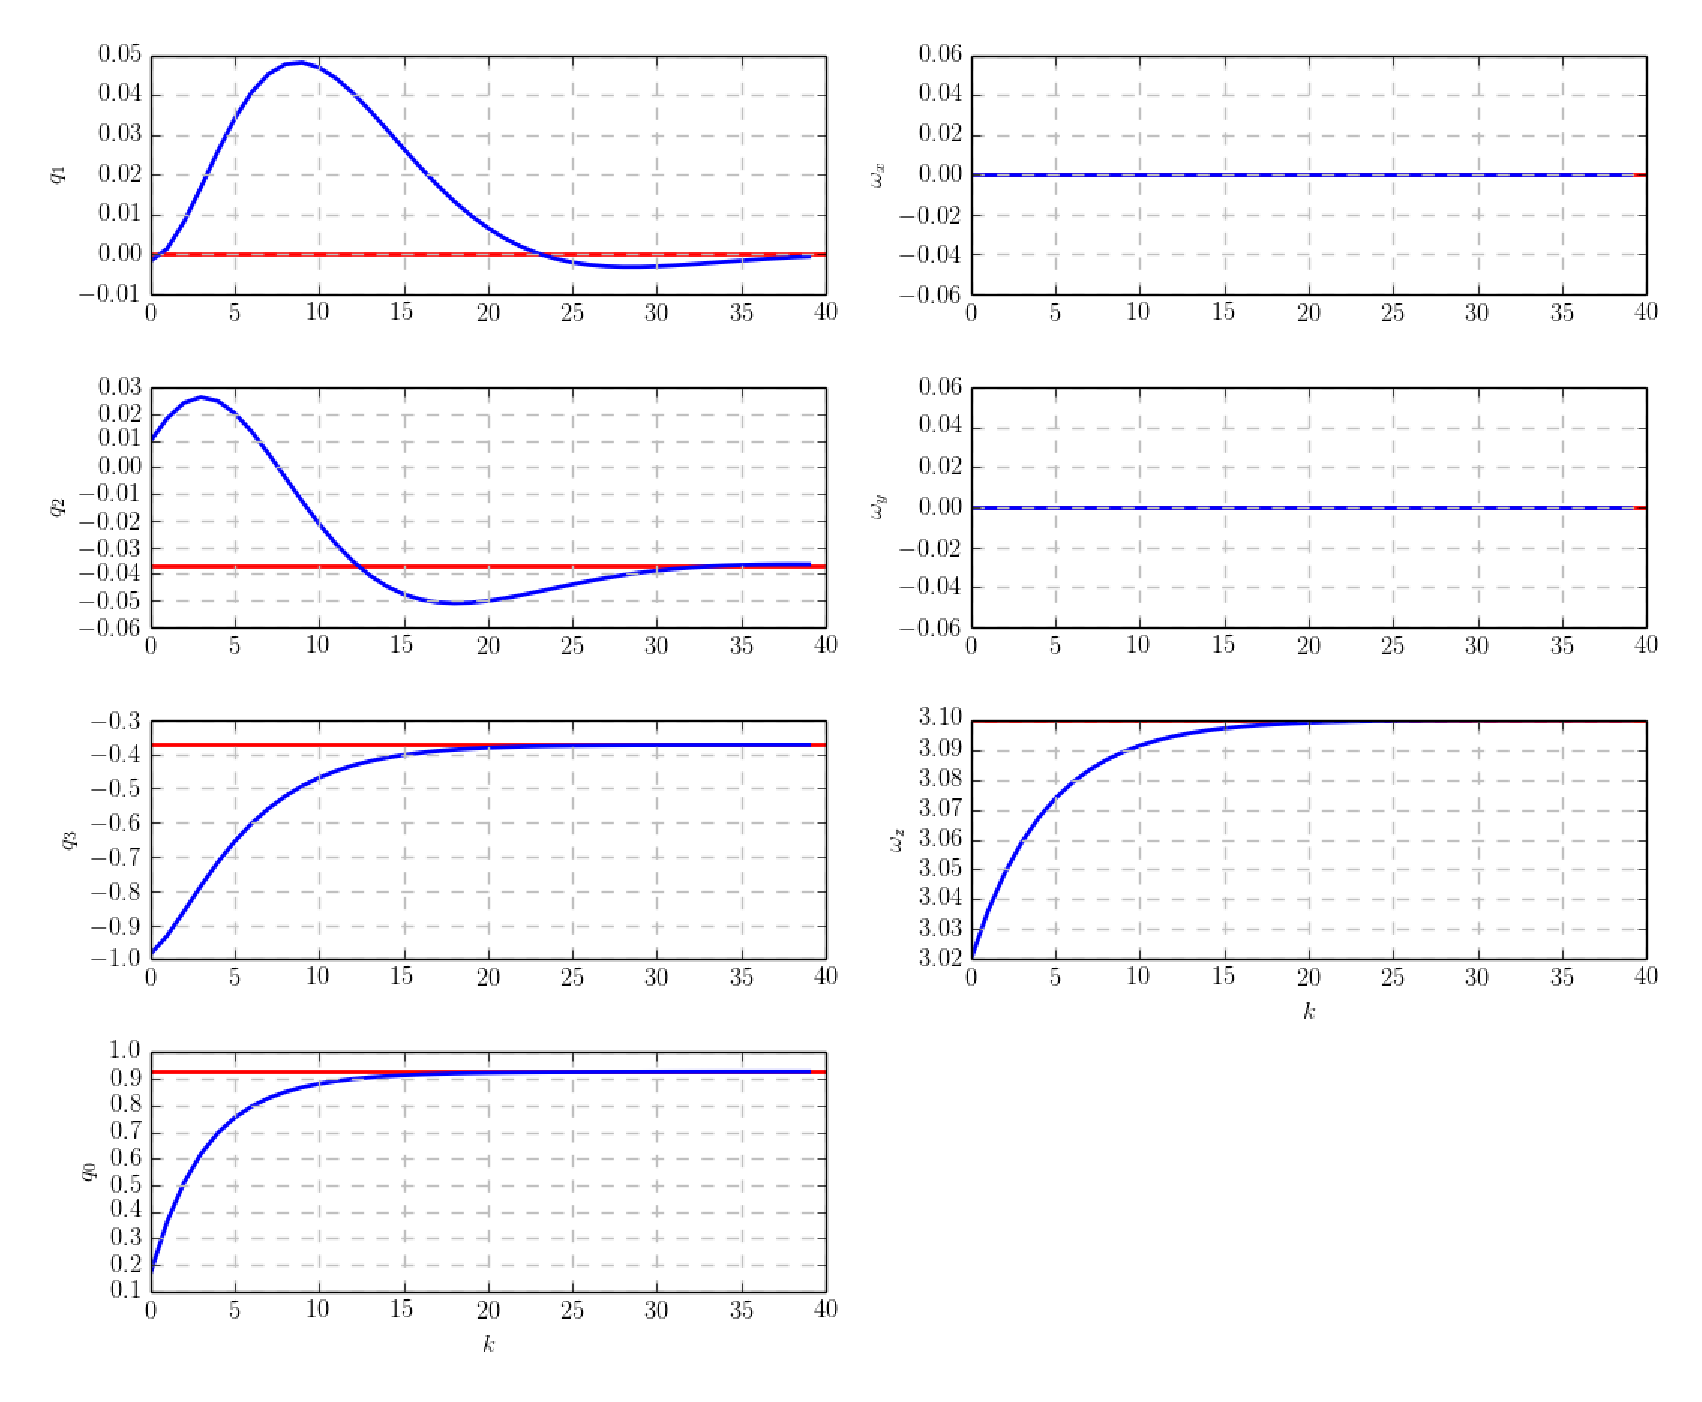
\psfig{file=figures/p_estimator_static_target.eps,width=6in}}
  \caption{P-Estimator with static target}
  \label{fig:PEstimatorwithstatictarget}
\end{figure}

The work covered so far in this chapter has all dealt with the a system in a static state.  In Figure \ref{fig:PEstimatorwithstatictarget}, a P-Estimator converges it's estimated state (blue) to the static measured state (red).  While the estimated state converges to the measured state after about 40 iterations, this type of conversion would be effective only for non-rotating systems.  The non-zero $\omega_z$ means that the quaternion attitude representation will be in constant motion.

The $3.1$ rad/sec rotation about $0\bs{i} + 0.1\bs{j} + 1\bs{k}$ condition from the previous p-estimator is then allowed to propagate the quaternion state through 10 second of rotation with state estimate updates every 0.1 sec.  The resulting measured state (red) and estimated state (blue) is shown in Figure \ref{fig:PEstimatorwithrotatingtarget}.  The body rates track identically to those in Figure \ref{fig:PEstimatorwithstatictarget} where $t(k) = 2$ corresponds to $k = 20$.  Due to the proportional only compensation and no predictive methods, the initial transient behavior is followed by a behavior similar to a steady state error.

\begin{figure}[H]
  \centerline{\psfig{file=figures/p_estimator_3radps.eps,width=6in}}
  \caption{P-Estimator with rotating target}
  \label{fig:PEstimatorwithrotatingtarget}
\end{figure}

Increasing the frequency of updates to the p-estimator can decrease the error between the measured and estimated states, but there will always be an error similar to a steady state error in the quaternion representation.  For better results the estimator needs to take into consideration changes in the state through the PID's integration and derivative terms.

\subsubsection{Integral Estimator}
\label{subsubsec:IntegralEstimator}

To stay consistent with the findings in the State Error section (\ref{sec:StateError}), the quaternion portion of the integrated state should abide by the quaternion multiplicative correction method.  This is the first model where the variable sized time step is also taken into consideration.  Instead of accumulating the error measurements, the error corrections should be weighted according to the length of time between updates $t(k+1) - t(k)$.  In a simplified case the integral term should end up the same in the following two update instances.

\begin{table}[H]
  \centering
  \begin{tabular}{r|c|c|c|c|c}
    $t_1 (sec)$ & 0.1 & 0.2 & 0.3 & 0.4 & 0.5 \\ \hline
    $\theta_e$ & 4 & -3 & -3 & -3 & 5 \\
    \\
    $t_2 (sec)$ & 0.1 & & & 0.4 & 0.5 \\ \hline
    $\theta_e$ & 4 &  &  & -3 & 5 \\
  \end{tabular}
  \label{tbl:VariableUpdates}
\end{table}

In $t_1$, regular updates occur every 0.1 sec ending in an integral error value of 0.  In $t_2$, without taking into consideration the variable step sizes would end in an error value of $+6$, but really the -3 error update should be worth three times as much.

Running the state estimator without compensating for variations in time step sizes can create inconsistencies between different experimental runs.  In Figure \ref{fig:IEstimatorwithouttimevariationcompensation}, the integral estimator was updated with a fixed state for 30 seconds.  The estimator was initialized at $0$ radians and run three times against a fixed angle of $0.5$ radians.  The first time with an estimation update frequency of every 0.4 seconds (blue), second with the update frequency of every 0.1 seconds (red), and third with a variable update frequency (green) that jumped back and forth between updating every 0.05 and 0.4 seconds.

\begin{figure}[H]
  \centerline{\psfig{file=figures/i_estimator_no_time_varying.eps,width=6in}}
  \caption{I-Estimator without time variation compensation}
  \label{fig:IEstimatorwithouttimevariationcompensation}
\end{figure}

Each calculated estimate for $\hat{\theta}$ in the $k$ domain is identical for each of the three runs, but varies greatly in the time domain.  Most notably, the third run that alternates between update frequencies ends up creating an estimation dynamic that could make the controller less robust.

In comparison, the PID estimator was modified to incorporate the time step size into it's integral term.  The same three tests were run as above with the 0.1 (red), 0.4 (blue), and variable 0.05/0.4 (green) time steps.  The adjustment quaternion method from Section \ref{subsec:RepresentativeStateAdjustments} is first used to compensate for measured time step size of $\Delta t_{k}$ creating a consistent error quaternion. then is used as before to scale the error quaternion by the selected gain value.  The results of this work can be seen in Figure \ref{fig:IEstimatorwithtimevariationcompensation} where the three test runs are still not identical, but their dynamics are more similar than before.  More notably, the variable step test (green) shows less variability in the estimate being produced which will reduce the noise being transferred to the control algorithm.

\begin{subequations}
  \begin{align}
    \bs{\hat{x}}(t_{k+1}) &= \begin{bmatrix} \bs{\hat{q}}(t_{k+1}) \\ \bs{\hat{\omega}}(t_{k+1}) \end{bmatrix} \\
    \bs{\hat{q}}(t_{k+1}) &= \bs{\psi}\big(\bs{q}_{ei}(t_k), K_{qi}\big) \otimes \bs{\hat{q}}(t_{k}) \\
    \bs{q}_{ei}(t_k) &= \bs{\psi}(\bs{q}_e(t_{k}), \Delta t_{k}) \otimes \bs{q}_{ei}(t_{k-1})\\
    \bs{\hat{\omega}}(t_{k+1}) &= \bs{\hat{\omega}}(t_{k}) + \bs{K}_{\omega i} \cdot (\Delta t_k \bs{I})\cdot \bs{\omega}_e(t_{k})
  \end{align}
  \label{eqn:IEstimator}
\end{subequations}

In Equation \ref{eqn:IEstimator}, the error quaternion $\bs{q}_{ei}(t_k)$ used is an accumulation of the time step scaled errors encountered in all previous steps.  This is analogous to a running summation of the error values.  For the body rate estimation, it's largely the traditional integral component with an extra $\Delta t_k \bs{I}$ term that linearly scales the body rate error calculations based on the size of the current time step.

\begin{figure}[H]
  \centerline{\psfig{file=figures/i_estimator_time_varying.eps,width=6in}}
  \caption{I-Estimator with time variation compensation}
  \label{fig:IEstimatorwithtimevariationcompensation}
\end{figure}

\subsubsection{Derivative Estimator}
\label{subsubsec:DerivativeEstimator}

The derivative component of the PID estimator takes a similar form to the integral component in Equation \ref{eqn:IEstimator}.  The derivative component is only concerned with the current error, previous error, and the current time step size.  As with the integral body rate correction, the derivative correction is scaled by $\frac{1}{\Delta t_k}$ to compensate for variable step sizes.

\begin{subequations}
  \begin{align}
    \bs{\hat{x}}(t_{k+1}) &= \begin{bmatrix} \bs{\hat{q}}(t_{k+1}) \\ \bs{\hat{\omega}}(t_{k+1}) \end{bmatrix} \\
    \bs{\hat{q}}(t_{k+1}) &= \bs{\psi}\left(\bs{q}_{ed}(t_k), K_{qd}\right) \otimes \bs{\hat{q}}(t_{k}) \\
    \bs{q}_{ed}(t_k) &= \bs{\psi}\left(\bs{q}_e(t_{k-1})^* \otimes \bs{q}_e(t_{k}), \frac{1}{\Delta t_{k}}\right)\\
    \bs{\hat{\omega}}(t_{k+1}) &= \bs{\hat{\omega}}(t_{k}) + \bs{K}_{\omega d} \cdot \left(\frac{1}{\Delta t_k} \bs{I}\right) \cdot \bs{\omega}_e(t_{k})
  \end{align}
  \label{eqn:DEstimator}
\end{subequations}

The Figures \ref{fig:DEstimatorwithouttimevariationcompensation} and \ref{fig:DEstimatorwithtimevariationcompensation} below are the results of three test runs with the same set up update frequencies as with the integral component (0.1/sec, 0.4/sec, and varied).  For this comparison, the TableSat was simulated into a steady $0.01$ rad/s rotation about the body $+z$-axis to generate a constant rate of change for the quaternion instead of the fixed quaternion in the integral test.  The $\theta_{adj}$ parameter tracked for this test is the angular rotation associated with the $\bs{\psi}\left(\bs{q}_{ed}(t_k), K_{qd}\right)$ quaternion adjustment term.

\begin{figure}[H]
  \centerline{\psfig{file=figures/d_estimator_no_time_varying.eps,width=6in}}
  \caption{D-Estimator without time variation compensation}
  \label{fig:DEstimatorwithouttimevariationcompensation}
\end{figure}

Figure \ref{fig:DEstimatorwithouttimevariationcompensation} shows the results of the test run without consideration taken for time step sizes.  With a constant spin rate, the resulting quaternion adjustment is tightly coupled to the frequency that the updates are made with the 0.1 (red), 0.4 (blue), and variable 0.05/0.4 (green) time steps.  The variable time step sequence is a particular concerns as it jumps back and forth between adjusted amount suggesting the spin rate is not constant.

\begin{figure}[H]
  \centerline{\psfig{file=figures/d_estimator_time_varying.eps,width=6in}}
  \caption{D-Estimator with time variation compensation}
  \label{fig:DEstimatorwithtimevariationcompensation}
\end{figure}

Figure \ref{fig:DEstimatorwithtimevariationcompensation} implements the time variation compensation in Equation \ref{eqn:DEstimator} where the quaternion adjustments provide a better representation of the measured constant spin rate.

\subsubsection{PID Estimation of Unforced Motion}
\label{subsubsec:PIDEstimatorofUnforcedMotion}

Combining the proportional, integral, and derivative estimator portions from above.  Equations \ref{eqn:PEstimator}, \ref{eqn:IEstimator}, and \ref{eqn:DEstimator} get combined into a single PID estimator as

\begin{subequations}
  \begin{align}
    \bs{\hat{x}}(t_{k+1}) &= \begin{bmatrix} \bs{\hat{q}}(t_{k+1}) \\ \bs{\hat{\omega}}(t_{k+1}) \end{bmatrix} \\
    \bs{\hat{q}}(t_{k+1}) &= \bs{\psi}\left(\bs{q}_{ed}(t_k), K_{qd}\right) \otimes \bs{\psi}\big(\bs{q}_{ei}(t_k), K_{qi}\big) \otimes \bs{\psi}(\bs{q}_e(t_{k}), K_{qp})  \otimes \bs{\hat{q}}(t_{k}) \\
    \bs{\hat{\omega}}(t_{k+1}) &= \bs{\hat{\omega}}(t_{k}) + \bs{K}_{\omega p} \cdot \bs{\omega}_e(t_{k}) + \bs{K}_{\omega i} \cdot (\Delta t_k \bs{I})\cdot \bs{\omega}_e(t_{k}) + \bs{K}_{\omega d} \cdot \left(\frac{1}{\Delta t_k} \bs{I}\right) \cdot \bs{\omega}_e(t_{k})
  \end{align}
  \label{eqn:PIDEstimatorUnforcedMotion}
\end{subequations}

The update to the estimated body rate follows the traditional method of the PID control with the addition of the scaling factors for the integral and derivative terms that compensate for non-uniform step sizes at run-time.  The quaternion correction is a compilation of the individual correction quaternions and joined through the multiplicative error correction method.

With a spin stabilized system controlling the body rate is relatively straight forward with a PID controller.  A test was run through TSatPy with based on the PID estimation in Equation \ref{eqn:PIDEstimatorUnforcedMotion}.  The system was set at a spin rate of $0.314$ rad/sec rotation about $+z$ with the measurement of the quaternion angle $\theta$ containing noise $N \sim (0, 0.1218)$ radians.  A gradient descent gain selection settled on the following parameters.

\begin{equation}
  \begin{aligned}
    K_{qp} &= 0.98, K_{qi} = 0.001, K_{qd} = 0.001 \\
    \bs{K}_{\omega p} &= 0.7 \bs{I}, \bs{K}_{\omega i} = \bs{0}, \bs{K}_{\omega d} = \bs{0}
  \end{aligned}
\end{equation}

The test run results are show in Figure \ref{fig:PIDEstimatorwithoutstateprediction}.  The bottom two graphs showing body rate tracking performance where the basic proportional control quickly brings the body rate error under control.  The quaternion estimations are much more difficult largely due to the lack of a system model to convert body rates to estimated attitudes at the next update.  Since the system is spin stabilized and the estimated quaternion has no prior knowledge of where the next value will be, it relies on a large proportional component to jump to the new measurement values on each update.

While testing the performance of the integral and derivative components showed an improved performance when incorporating the effects of the variable time step, in this test with such a heavy reliance on the proportional component, the benefits to considering the variable time step effects were negligible.

\begin{figure}[H]
  \centerline{\psfig{file=figures/pid_estimator_no_prediction_high_P.eps,width=6in}}
  \caption{PID-Estimator without state prediction}
  \label{fig:PIDEstimatorwithoutstateprediction}
\end{figure}

\subsection{State Prediction}
\label{subsec:StatePrediction}

Section \ref{subsec:PIDEstimation} shows that to keep accurate tracking of a spin stabilized satellite like TableSat or MMS, the system's dynamic equations are required to couple the body rate and quaternion values.  This is especially important for the TableSat 1A implementation since only the magnetometer and course sun sensors provide feedback about the system's state, and they only have a partial measurement of the attitude quaternion and no direct measurement of the body rates.

The approach taken in the TSatPy code to create state predictions off previous state estimates is to start with a discretized Euler's Moment Equations \ref{eqn:DiscreteEulerMomentEquations} to predict $\bs{\dot{\omega}}(t_{k+1})$.  The the current estimated body rate is adjusted based on the variable time step size.

\begin{equation}
  \bs{\omega}(t_{k+1}) = \bs{\omega}(t_{k}) + \bs{\dot{\omega}}(t_{k+1})\cdot (t_{k+1} - t_k)
\end{equation}

The newly estimated body rates $\bs{\omega}(t_{k+1})$ are supplied to the discretized quaternion dynamics Equation \ref{eqn:DiscreteQuaternionPropagation} to calculate the newly estimated rotational quaternion.

\subsection{PID Estimation with State Prediction}
\label{subsec:PIDEstimatorwithStatePrediction}

From Section \ref{subsec:PIDEstimation}, Equation \ref{eqn:PIDEstimatorUnforcedMotion} defines a method of tracking unforced spin stabilized satellites through PID state estimation.  The biggest issue was a heavy reliance on the proportional gain to track the quaternion attitude which is sensitive to measurement noise.  Incorporating a multiplicative-correction quaternion based model of rigid body dynamics based on the equations in Chapter \ref{chap:SatelliteAttitudeModeling} can assist in predicting the $t_{k+1}$ state of the system.

\begin{subequations}
  \begin{align}
    \bs{\hat{x}}(t_{k+1}) &= \begin{bmatrix} \bs{\hat{q}}(t_{k+1}) \\ \bs{\hat{\omega}}(t_{k+1}) \end{bmatrix} \\
    \bs{\hat{q}}(t_{k+1}) &= \bs{\psi}\left(\bs{q}_{ed}(t_k), K_{qd}\right) \otimes \bs{\psi}\big(\bs{q}_{ei}(t_k), K_{qi}\big) \otimes \bs{\psi}(\bs{q}_e(t_{k}), K_{qp})  \otimes \bs{\hat{q}}(t_{k+1})^- \\
    \bs{\hat{\omega}}(t_{k+1}) &= \bs{\hat{\omega}}(t_{k+1})^- + \bs{K}_{\omega p} \cdot \bs{\omega}_e(t_{k}) + \bs{K}_{\omega i} \cdot (\Delta t_k \bs{I})\cdot \bs{\omega}_e(t_{k}) + \bs{K}_{\omega d} \cdot \left(\frac{1}{\Delta t_k} \bs{I}\right) \cdot \bs{\omega}_e(t_{k})
  \end{align}
  \label{eqn:PIDEstimatorwithPredictionUnforcedMotion}
\end{subequations}

with the a priori state $\bs{\hat{x}}(t_{k+1})^-$ as

\begin{equation}
  \bs{\hat{x}}(t_{k+1})^- = \begin{bmatrix}\bs{\hat{q}}(t_{k+1})^- \\ \bs{\hat{\omega}}(t_{k+1})^- \end{bmatrix} = f \Big( \bs{\hat{q}}(t_{k}), \bs{\hat{\omega}}(t_{k}) \Big)
\end{equation}

The PID estimator now with a state prediction method was run under the same testing conditions present in Figure \ref{fig:PIDEstimatorwithoutstateprediction}.  The resulting performance showed that the inclusion of the system model greatly reduced the reliance on the proportional component of the PID estimator which reduced the noise and increased the accuracy of the final estimates being provided to the controller.  The results in Figure \ref{fig:PIDEstimatorwithstateprediction} show the improved quaternion angle estimates when run with the following gains.

\begin{equation}
  \begin{aligned}
    K_{qp} &= 0.0735, K_{qi} = 0.000863, K_{qd} = 0.00812 \\
    \bs{K}_{\omega p} &= 0.7 \bs{I}, \bs{K}_{\omega i} = \bs{0}, \bs{K}_{\omega d} = \bs{0}
  \end{aligned}
\end{equation}

The quaternion's proportional value is still the dominant gain, but has been reduced by 92.5\% of it's previous value while still providing about 80\% reduction in quaternion attitude error rates.

\begin{figure}[H]
  \centerline{\psfig{file=figures/pid_estimator_with_prediction.eps,width=6in}}
  \caption{PID-Estimator with state prediction}
  \label{fig:PIDEstimatorwithstateprediction}
\end{figure}


\subsection{Sliding Mode Observer}
\label{subsec:SlidingModeObserver}

The Sliding Mode Observer (SMO) is a proportional estimator with an additional smoothing term that uses a chosen sliding surface.  The general form for the SMO is

\begin{equation}
  \bs{\dot{\hat{x}}} = \bs{\hat{f}}(\bs{\hat{x}}, \bs{\hat{u}}, t) + \bs{L}(\bs{C}\bs{\hat{x}} - \bs{C}\bs{x}) + \bs{K}\bs{1}_s\bs{\hat{y}}
  \label{eqn:SMOContinuous}
\end{equation}

Where L is a luenberger gain and $\bs{1}_s$ is a switching function based on $s$.  The sliding mode terms allow additional control of the state adjustments without adding a lot of computational complexity.  The SMO can continue to use the nonlinear model's state predictions as in the PID estimators in Section \ref{subsec:PIDEstimatorwithStatePrediction}, which is an advantage over methods such as the Extended Kalman Filter (EKF) where the system is linearized about an operating point and assumes a constant time step.

This thesis takes the discretized form of Equation \ref{eqn:SMOContinuous} with a quaternion multiplicative correction

\begin{subequations}
  \begin{align}
    \bs{\hat{x}}(t_{k+1}) &= \begin{bmatrix} \bs{\hat{q}}(t_{k+1}) \\ \bs{\hat{\omega}}(t_{k+1}) \end{bmatrix} \\
    \bs{\hat{q}}(t_{k+1}) &= \bs{\psi} (\bs{1}_s\big(\bs{q}_{e}(t_k)\big), K_q) \otimes \bs{\psi}(\bs{q}_e(t_{k}), L_{q})  \otimes \bs{\hat{q}}(t_{k+1})^- \\
    \bs{\hat{\omega}}(t_{k+1}) &= \bs{\hat{\omega}}(t_{k+1})^- + \bs{L}_{\omega} \bs{\omega}_e(t_{k}) + \bs{K}_{\omega}\bs{1}_s \big(\bs{\omega}_e(t_{k}) \big)
  \end{align}
  \label{eqn:SMOEstimatorwithPredictionUnforcedMotion}
\end{subequations}

where

\begin{subequations}
  \begin{align}
    \bs{1}_s\big(\bs{q}_{e}(t_k) \big) &= \begin{bmatrix} \bs{v_e} \\ sat\left( \frac{2\cos^{-1} q_{0e} }{S_{q}} \right) \end{bmatrix} \\
    \bs{1}_s \big(\bs{\omega}_e(t_{k}) \big) &= sat\left( \frac{\bs{\omega}_e(t_{k})}{S_{\omega}} \right) \\
    \bs{L}_{\omega} &= L_\omega \cdot \bs{I} \\
    \bs{K}_{\omega} &= K_\omega \cdot \bs{I}
  \end{align}
\end{subequations}

For body rates, the a priori state provides the predicted body rate $\bs{\hat{\omega}}(t_{k+1})^-$ that gets adjusted by a proportional term $\bs{L}_{\omega} \bs{\omega}_e(t_{k})$ as in the P-Estimator, but has an additional saturation function correction based on sliding surfaces for the individual body rate errors.  As found in the PID estimator, the proportional estimator for a steady spin stabilized satellite performs adequately.  The additional saturation term becomes helpful for situations with low $L_\omega$ values that can take longer to converge from the initial body rate to the actual body rate, but once close will increase the effort in staying in step with the measured body rate.

Similar to the PID estimator, the quaternion sliding mode observer limits it's focus to the angular measure of the rotational quaternion.  The sliding surface is taken based on the radian measure.  If the radian measure is below, the saturation limit the quaternion stays as is.  If the quaternion represents a rotation greater than the saturation limit a saturated quaternion is created about the same Euler axis but limit to the saturation angle of rotation.

Running the same tests as run against the PID estimators, the following parameters were located through an iterative gradient descent method that minimized the quaternion error angle and standard deviation of the error angle.

\begin{equation}
  \begin{aligned}
    L_q = 0.362 &, L_w = 0.375 \\
    K_q = 0.308 &, K_w = 0.499 \\
    S_q = 0.419 &, S_w = 0.00517 \\
  \end{aligned}
\end{equation}

Figure \ref{fig:SMOEstimatorwithstateprediction} shows the result of the test at these optimized parameters.  The inverted angle measurement in the first graph is an artifact of the non-unique representation of a quaternion attitude.  In this case, the estimated angles are being calculated for rotations about the body's $-z$-axis instead of the $+z$ axis.  This further supports the decision made in Section \ref{sec:StateError} to use the multiplicative error as the second graph shows the correct error values.

Although the SMO in this case is able to traverse the initial transient response well, the steady state quaternion error is almost as high as using a PID estimator with no state prediction method.  This behavior is due to the high quaternion measurement noise.  With the saturation function, the sliding mode observer is still largely a proportional estimator without the assistance of an integral term to smooth out the noise.

\begin{figure}[H]
  \centerline{\psfig{file=figures/smo_estimator_with_prediction.eps,width=6in}}
  \caption{SMO-Estimator with state prediction}
  \label{fig:SMOEstimatorwithstateprediction}
\end{figure}

Based on these results, the SMO performs acceptably for the body rate estimation, but according to the steady state error rates, it appears that the PID estimation would be a better use for the steady state attitude tracking.  Both estimators have similar performance profiles which makes it more complicated to determine the better choice.  Section \ref{subsec:ComparativeEstimationTests} will go over how TSatPy can assist with running both estimation techniques in parallel for to provide a more accurate representation.

\subsection{Comparative Estimation Tests}
\label{subsec:ComparativeEstimationTests}

One of the advantages to developing the TSatPy code base for the MMS/TableSat spin stabilized is the ability to run a comparative analysis of multiple estimators at the same time.  The estimators run agnostic to the source of the measurements.  In the sample shown below, the state measurements were generated by a model, but could also be switched to be pulled off the TableSat.

Figure \ref{fig:PIDSMOEstimatorConcurrentComparison} was generated by running a single simulation an providing the truth model's measured state to both a PID and SMO estimator tuned to the parameters selected during individual gain tuning tests above.  This allows for a clear side-by-side comparison of their performance.  Multiple runs all have similar characteristics.  In the initial transient response both estimators are able to converge to a steady state after just a couple updates, but the SMO is able to converge slightly faster each time.  For the steady state response the PID estimator consistently maintains a lower average error, although with a slightly higher standard deviation.  As with the initial response, the SMO estimation values generally update slightly just before the PID estimator.

\begin{figure}[H]
  \centerline{\psfig{file=figures/estimator_comparison.eps,width=6in}}
  \caption{PID/SMO Estimator Concurrent Comparison}
  \label{fig:PIDSMOEstimatorConcurrentComparison}
\end{figure}

The results in Figure \ref{fig:PIDSMOEstimatorConcurrentComparison} were generated through the TSatPy application with the script below.  Lines 10-15 define the two estimators to use in the simulation.  More can be added including the same estimator type with varied parameters.  Lines 17-19 define the system clock behavior.  The simulation will run for a simulated 120 seconds as verified in the results above.  The time steps for each update will vary between 0.8 and 1.2 seconds randomly.  And since this is running as a simulation instead of pulling data from the physical TableSat, the clock can be sped up to run at 10x speed improving the rate of the iterative testing cycle.

\begin{singlespace}
  \begin{minted}[mathescape,linenos,numbersep=10pt,frame=lines,framesep=2mm]{python}
from TSatPy import Estimator, State
from TSatPy.Clock import Metronome
import numpy as np
import matplotlib.pyplot as plt
import time
import random

print('PID / SMO Faceoff')

configs = [{'type': 'pid',
 'args': {'kpq': 0.0735,'kpw': 0.7,'kiq': 0.000863,
          'kiw': 0,'kdq': 0.00812,'kdw': 0}
},{'type': 'smo',
 'args': {'Lq': 0.3619,'Lw': 0.3752,'Kq': 0.3076,
           'Kw': 0.4994,'Sq': 0.4191,'Sw': 0.0052}}]

run_time = 120
speed = 10
dts = [0.8, 1.2]
c = Metronome()
c.set_speed(speed)
I = [[2, 0,  0], [0, 2, 0], [0, 0, 2]]

def setup_estimators(configs):
    x_ic = State.State()
    plant_est = State.Plant(I, x_ic, c)

    est = Estimator.Estimator(c)
    for config in configs:
        est.add(config['type'], plant_est, config['args'])

    return est

def run_comparison(est):
    x_ic = State.State(
        State.Quaternion([0,0,1], radians=4),
        State.BodyRate([0,0,0.314]))
    plant = State.Plant(I, x_ic, c)

    ts = []; smo_err = []; pid_err = []
    start_time = c.tick()
    end_time = c.tick() + run_time
    while c.tick() < end_time:
        plant.propagate()
        offset = np.random.randn() * 20 / 180.0 * np.pi
        q_noise = State.Quaternion([0,0,1], radians=offset) * plant.x.q

        x_m = State.State(q_noise, plant.x.w)

        est.update(x_m)
        ts.append(c.tick() - start_time)

        for model in est.estimators:
            q_e = State.QuaternionError(model.x_hat.q, plant.x.q)
            e, r = q_e.to_rotation()

            if type(model) is Estimator.PID:
                pid_err.append(r)
            elif type(model) is Estimator.SMO:
                smo_err.append(r)
        random.shuffle(dts)
        time.sleep(dts[0] / float(speed))

    return ts, pid_err, smo_err

def graph_it(ts, pid_err, smo_err):
    # Generate the graph here
    # See appendix for the full script

def main():
    est = setup_estimators(configs)
    graph_it(*run_comparison(est))
    return 0

if __name__ == '__main__':
    exit(main())
  \end{minted}
\nocite{minted}
\end{singlespace}

\section{Controllers}
\label{sec:Controller}

The TableSat 1A controller has performance requirements based off of NASA MMS's mission parameters.  Section \ref{subsec:ComparativeEstimationTests} demonstrated that multiple estimators can be run in parallel during both simulations and experimental runs.  As discussed above, this allows for a better insight into performance differences in estimation methods.  An additional benefit to running the controller through TSatPy is the ability to perform estimator scheduling.  Like gain scheduling which for an estimator or controller can modify what gains it uses depending on the current performance, estimator scheduling allows for switching between disparate estimation techniques during run-time.  For example, one estimator tuned for responding to large errors and run along side an estimator tuned for steady state performance.  The control algorithm can then receive more accurate state estimates on a wider range of environmental conditions.

The control requirements for TableSat 1A can be simplified into three main goals.

First is to maintain a steady spin rate of 3 rpm (0.31416 rad/sec).  Given the relative success of the body rate estimation in section \ref{sec:Estimators}, this goal should not be that difficult and likely will not need a complicated control model.

Second is to correct for any nutation out of the spin plane detected by the estimator.  This can take the form of both driving body rates $\omega_y$ and $\omega_z$ to zero, and ensuring the estimated quaternion has an Euler axis is kept in parallel with the global $z$-axis.

Third is to prevent oscillations in the ADP and SDP booms or attenuate any existing oscillations.  Out of the three, this performance goal has the largest set of dependencies for success.  This level of control is reliant on effective actuators along with reliable state estimates based on an accurate system model including boom dynamics.

\subsection{Actuators}
\label{subsec:Actuators}

The actuators in use on TableSat 1A consists of four single directional computer fans.  Two oriented for rate control and two for nutation corrections.  Rate control fans are mounted on opposite sides of the deck in opposing directions.  The two nutation fans are mounted at 90 degree angles and both have their thrust pointing down.  The fans are assumed to be mounted so that the rotation and nutation moments are applied about orthogonal axes, and that the thrust applied is tangential to the body's center of mass.  This initially simplifies the controller's voltage calculations for each fan which can be revisited if testing shows the effects are not negligible.

\begin{figure}[H]
  \centerline{\psfig{file=figures/tsat_thrusters.eps,height=3in}}
  \caption{TableSat 1A thrusters}
  \label{fig:TSatThrusters}
\end{figure}

With this arrangement, actuators are identified by their center, direction of thrust related to the body reference frame, and the maximum force the actuator can produce.

\begin{figure}[H]
  \centerline{\psfig{file=figures/tsat_body_axes.eps,height=3in}}
  \caption{TableSat Body Axes}
  \label{fig:TableSatBodyAxes}
\end{figure}

\begin{table}[H]
  \centering
  \begin{tabular}{c|c|c|c|c}
    Fan & Center $\bs{f_c}$ (m) & Direction $\bs{n}$ & $F$ (N) & Max Moment $\frac{F \bs{n} \times \bs{f_c}}{|\bs{n}|}$ (Nm) \\ \hline
    1 & $(0.2474, -0.2474, 0)$ & $(-1, -1, 0)$ & 0.08 & $(0, 0, 0.039598)$ \\
    2 & $(-0.2474, 0.2474, 0)$ & $(-1, -1, 0)$ & 0.08 & $(0, 0, -0.039598)$ \\
    3 & $(0.25, 0, 0)$ & $(0, 0, -1)$ & 0.08 & $(0.02, 0, 0)$ \\
    4 & $(0, 0.25, 0)$ & $(0, 0, -1)$ & 0.08 & $(0, -0.02, 0)$ \\
  \end{tabular}
  \caption{Actuator configuration}
  \label{tbl:ActuatorConfiguration}
\end{table}


The role of the actuator module is to accept a desired moment in $\Re^3$ about the body's frame of reference and return what moment is capable with the limited actuator configuration and single direction fans.  The configuration listed in lines 4-13 represent the fan configuration displayed in Figure \ref{fig:TSatThrusters} with the addition of a hypothetical second clockwise fan to demonstrate how the request can be distributed among multiple fans if available.

In the ``setup\_actuators'' function, each fan configuration is fed into the module which calculates the maximum possible moment using the fan's location, direction, and force.

\begin{equation}
  M = \frac{F \bs{n} \times \bs{f_c}}{|\bs{n}|}
\end{equation}

Lines 31-36 list the potential moments for each of the actuators loaded.  Lines 26-28 simulate a request by the controller module for a $(0.03, 0.01, 0.07)$ Nm moment.  Since the fans are mounted to create moments about one of the body reference frame axes, each component of the request is considered separately.  The $M_x = 0.03 Nm$ request can only be partially fulfilled by the Nx fan at max thrust producing a $0.02 Nm$ moment.  The $M_y = 0.01 Nm$ request is within the limits of the Ny fan but because the fan is single directional, the request can not be filled.  The $M_z = 0.07 Nm$ request can not be served by either the CCW1 or CCW2 fans alone but can be generated by both fans if they share the load.  The actuator module splits the request equally between the two CCW fans at 88\% of their max capacity.  In the end, of the initial $(0.03, 0.01, 0.07) Nm$ request is reduced to an attainable moment of $(0.02, 0, 0.07) Nm$.  At this point the information is provided to both``set\_level'' function that would relay the appropriate voltage requirements to the TableSat.  To finish up the request, the actuator module returns the attained moment which can enter a feedback to the estimator and control modules for more accurate system modeling.

\begin{singlespace}
  \begin{minted}[mathescape,linenos,numbersep=10pt,frame=lines,framesep=2mm]{python}
import numpy as np
from TSatPy.Actuator import Actuator

configs = [{'type': 'fan', 'args': {'name': 'CW',
  'center': (0.2474, -0.2474, 0), 'direction': (-1, -1, 0), 'F': 0.08}
},{'type': 'fan', 'args': {'name': 'CCW1',
  'center': (-0.2474, 0.2474, 0), 'direction': (-1, -1, 0), 'F': 0.08}
},{'type': 'fan', 'args': {'name': 'CCW2',
  'center': (-0.2474, -0.2474, 0), 'direction': (1, -1, 0), 'F': 0.08}
},{'type': 'fan', 'args': {'name': 'NY', 'center': (0.25, 0, 0),
  'direction': (0, 0, 1), 'F': 0.08}
},{'type': 'fan', 'args': {'name': 'NX', 'center': (0, 0.25, 0),
  'direction': (0, 0, 1), 'F': 0.08}}]

def set_level(act, power_level):
    print 'Setting power level=%g for: %s' % (power_level, act)

def setup_actuators(configs):
    act = Actuator()
    for config in configs:
        act.add(config['type'], set_level, config['args'])
    return act

act = setup_actuators(configs)
print(act)
M = np.mat([0.03, 0.11, 0.07]).T
print("Request moment: %s" % (M.T))
print("Applied moment: %s" % (act.request_moment(M).T))

# Prints Out
# Actuator
#  <Fan CW moment=(0, -0, -0.0279901)>
#  <Fan CCW1 moment=(0, 0, 0.0279901)>
#  <Fan CCW2 moment=(0, 0, 0.0279901)>
#  <Fan NY moment=(0, -0.02, 0)>
#  <Fan NX moment=(0.02, 0, 0)>
# Request moment: [[ 0.03  0.11  0.07]]
# Setting power level=1 for: <Fan NX moment=(0.02, 0, 0)>
# Setting power level=1 for: <Fan CCW1 moment=(0, 0, 0.0279901)>
# Setting power level=1 for: <Fan CCW2 moment=(0, 0, 0.0279901)>
# Applied moment: [[ 0.02        0.          0.05598023]]
  \end{minted}
\nocite{minted}
\end{singlespace}

Prior implementations of TableSat generally stuck with a static actuator layout which requires a significant portion of time to rewrite code and/or rewire electronics to assess variations on the actuator layout.  With the use of TSatPy, most modifications to the actuators during testing can be done with just a change to the config structure that provides a much faster turn around time between tests.

\subsection{Rate Control}
\label{subsec:RateControl}

The first of the three controls goals introduced at the start of Section \ref{sec:Controller}, is the rate control of the TableSat/MMS to control the $\omega_z$ body rate at a slow and steady $0.314$ rad/s while any body rates about the $\omega_x$ and $\omega_z$ axes be removed.  The rate controller works on the premise of accepting the estimator's guess at the state of the system and comparing that to a desired state.  Correction moments, $\bs{M}$, are calculated based on any differences in the estimated and desired states.

\begin{equation}
  \bs{M}(t_{k+1}) = f(\bs{\hat{x}}(t_{k+1}), \bs{x}_d, t)
  \label{eqn:GeneralRateControl}
\end{equation}

\subsubsection{PID Rate Control}
\label{subsubsec:PIDRateControl}

A PID rate controller works very similar to the PID estimator.  The input to the estimator is two states with one composite state as the output.  The PID controller takes two states as input as well, but creates moments about the principle axes $M_x, M_y, M_z$.

\begin{equation}
  \bs{M}_{\omega}(t_{k+1}) = \bs{K}_{\omega p} \left( \bs{\omega}_d - \bs{\hat{\omega}}(t_{k+1}) \right)
  \label{eqn:PIDRateControl}
\end{equation}

A proportional controller governed by Equation \ref{eqn:GeneralRateControl} is more than adequate level of control for a system with perfect measurements since the proportional component is not corrupted by noise.  Figure \ref{fig:PRateControl} shows the response to a randomly assigned initial body rates and how they converge to the desired state of $\omega_z = 0.314$ rad/sec, $\omega_x = \omega_y = 0$ rad/sec, and the proportion gain of

\begin{equation}
  \bs{K}_{\omega p} = \begin{bmatrix} 0.404 & 0 & 0 \\ 0 & 0.463 & 0 \\ 0 & 0 & 0.428 \end{bmatrix}
\end{equation}

\begin{figure}[H]
  \centerline{\psfig{file=figures/p_rate_control.eps,width=6in}}
  \caption{P rate control}
  \label{fig:PRateControl}
\end{figure}

Expanding the proportional controller to include the integral and derivative term as shown in Equation \ref{eqn:PIDRateControl} can improve the performance slightly.  The addition correction terms generally reduce the overshoot of the response, but do not significantly shorten the time to bring the system to a steady state.

\begin{equation}
  \begin{aligned}
    \bs{M}_{\omega}(t_{k+1}) &= \bs{K}_{\omega p} \bs{\omega}_e(t_{k+1}) + \bs{K}_{\omega i} \cdot (\Delta t_k \bs{I})\cdot \bs{\omega}_e(t_{k+1}) + \bs{K}_{\omega d} \cdot \left(\frac{1}{\Delta t_k} \bs{I}\right) \cdot \bs{\omega}_e(t_{k+1}) \\
    \bs{\omega}_e(t_{k+1}) &= \bs{\omega}_d - \bs{\hat{\omega}}(t_{k+1}) \\
  \end{aligned}
  \label{eqn:PRateControl}
\end{equation}

\begin{figure}[H]
  \centerline{\psfig{file=figures/pid_rate_control.eps,width=6in}}
  \caption{PID rate control}
  \label{fig:PIDRateControl}
\end{figure}

The response curve in Figure \ref{fig:PIDRateControl} was generated with a random initial condition, and with the PID gains (Equation \ref{PIDRateControlGains}) tuned through a gradient descent iteration based off the total control effort.

\begin{subequations}
  \begin{align}
    \bs{K}_{\omega p} &= \begin{bmatrix} 0.597 & 0 & 0 \\ 0 & 0.643 & 0 \\ 0 & 0 & 0.450 \end{bmatrix} \\
    \bs{K}_{\omega i} &= \begin{bmatrix} 0.364 & 0 & 0 \\ 0 & 0.372 & 0 \\ 0 & 0 & 0.328 \end{bmatrix} \\
    \bs{K}_{\omega d} &= \begin{bmatrix} 0.435 & 0 & 0 \\ 0 & 0.357 & 0 \\ 0 & 0 & 0.392 \end{bmatrix}
  \end{align}
  \label{PIDRateControlGains}
\end{subequations}

\subsubsection{Sliding Mode Controller}
\label{subsubsec:SlidingModeController}

The Sliding Mode Controller (SMC) has a similar format to the Sliding Mode Observer (SMO) in Section \ref{subsec:SlidingModeObserver}.  Since the estimator contains a state prediction component, it is not required in the controller, and since the attitude is not under consideration for the rate controller, the quaternion adjustment terms are also removed.

\begin{subequations}
  \begin{align}
    \bs{M}_{\omega}(t_{k+1}) &= \bs{L}_{\omega} \bs{\omega}_e(t_{k+1}) + \bs{K}_{\omega}\bs{1}_s \big(\bs{\omega}_e(t_{k+1}) \big)
  \end{align}
  \label{eqn:SMOEstimatorwithPredictionUnforcedMotion}
\end{subequations}

where

\begin{equation}
  \bs{1}_s \big(\bs{\omega}_e(t_{k+1}) \big) = sat \begin{bmatrix} \omega_{ex}(t_{k+1}) / S_{\omega} &0 &0 \\ 0 & \omega_{ey}(t_{k+1}) / S_{\omega} & 0 \\ 0 & 0 & \omega_{ez}(t_{k+1}) / S_{\omega} \end{bmatrix}
\end{equation}

Unlike the comparison of the PID estimator with the Sliding Mode Observer where they're performances were very similar, the parameter tuned SMC clearly out performs the parameter tuned PID controller for rate control with perfect estimates.  Figure \ref{fig:SMCRateControl} shows the response of the rate control SMC where the response time is approximately half the time of the PID controller, and also with consistently less overshoot.

\begin{figure}[H]
  \centerline{\psfig{file=figures/smc_rate_control.eps,width=6in}}
  \caption{SMC rate control}
  \label{fig:SMCRateControl}
\end{figure}

The SMC in Figure \ref{fig:SMCRateControl}, was run with the following parameters tuned through a gradient descent algorithm.

\begin{equation}
    \bs{L}_{\omega} = \begin{bmatrix} 0.370 & 0 & 0 \\ 0 & 0.508 & 0 \\ 0 & 0 & 0.451 \end{bmatrix},
    \bs{K}_{\omega} = \begin{bmatrix} 0.428 & 0 & 0 \\ 0 & 0.424 & 0 \\ 0 & 0 & 0.549 \end{bmatrix},
    S_{\omega} = 0.511
  \label{SMCRateControlGains}
\end{equation}

While the SMC seems the clear preference for rate control, the two methods will need to be reevaluated when combined with each of the estimation techniques running off of noisy measurements.

\subsection{Nutation Correction}
\label{subsec:NutationCorrection}

Section \ref{subsubsec:PIDRateControl} covered the design of the rate controller which addresses the first goal of the controller to maintain a spin rate of $\omega_z = 3$ rpm.  This section will focus on the nutation control problem that to simplicity the overall controller design is decoupled from the rate control.  The combined control effort would be

\begin{equation}
    \bs{M}(t_{k+1}) = \bs{M}_{q}(t_{k+1}) + \bs{M}_{\omega}(t_{k+1})
\end{equation}

The nutation control will focus or the differences between the estimated quaternion attitude and the desired quaternion attitude.  The addition of the desired body rates of $\omega_x = \omega_y = 0$ can be added later if needed.  Since the work in Section \ref{sec:StateError} shows that working with the radian measure of the rotational quaternion had significant benefits over the traditional full state difference method, a similar approach will be used for the nutation control.

\subsubsection{P Nutation Control}
\label{subsubsec:PNutationControl}

Starting with a simplest design of the proportional nutation control where the error quaternion $\bs{q}_e$ is defined in terms of the estimated quaternion $\bs{\hat{q}}$ and the desired quaternion attitude $\bs{q}_d$ as

\begin{equation}
  \bs{q}_e = \bs{\hat{q}}^* \otimes \bs{q}_d
\end{equation}

To generate the moments needed to correct for the error in attitude, the P controller can take advantage of the quaternion notation where the vector portion identifies the Euler axis, and whose components can be used as the basis for the correction moment by scaling them by the radian angular measurement of the error and a proportional gain.

\begin{subequations}
  \begin{align}
    \bs{M}_{q}(t_{k+1}) &= (-2 K_{qp} \cos^{-1} (\hat{q}_{e0})) \bs{\hat{e}}_e \\
    \text{where } \bs{\hat{e}}_e &= \frac{\bs{\hat{v}}_e}{|\bs{\hat{v}}_e|}
  \end{align}
  \label{eqn:PNutationControl}
\end{subequations}

To assess the basic functionality of the proportional quaternion in Equation \ref{eqn:PNutationControl}, the controller was run with $K_{qp} = 0.01$ and told to return the quaternion to the standard state with the body's reference frame aligned with the global reference frame.  The TableSat was given an initial condition of

\begin{subequations}
  \begin{align}
    \bs{\hat{v}}_e &= 0\bs{i}+0.1\bs{j}+1 \bs{k}\\
    \theta &= 1 \text{ rad} \\
    \bs{\omega} &= \begin{bmatrix} 0 \\ -0.01 \\ 0.2 \end{bmatrix} \text{ rad/sec}
  \end{align}
\end{subequations}

\begin{figure}[H]
  \centerline{\psfig{file=figures/p_attitude_control.eps,width=6in}}
  \caption{P Attitude Control}
  \label{fig:PAttitudeControl}
\end{figure}

The results shown in \ref{fig:PAttitudeControl} are very promising.  The three dimensional object with an initial out of plane offset and initial body rates is able to oscillate about the desired set point with the use of a single gain measure being combined with the components of the quaternion state.









Assuming the system has been brought up to the desired operating conditions, there are a minimum of two checks that are required to determine if the system continues to stay in the desired state.

\begin{equation}
  \begin{aligned}
    \omega_z &= 3 \text{ rpm} \\
    \bs{v} \bullet (0\bs{i}+0\bs{j}+1\bs{k}) &= \left\{ \begin{array}{lr} 1 & : q_0 > 0 \\ -1 & : q_0 < 0 \end{array} \right.
  \end{aligned}
  \label{}
\end{equation}

Correcting for variations in $\omega_z$ follows standard control theory methods.  Correcting for variation in the Euler vector are more complicated especially when keeping with multiplicative correction methods instead of state difference methods as was determined in Section \ref{sec:StateError}.  Keeping the two state requirements decoupled is advantageous if possible.  Even though the rate of the quaternion can be used to help control the body rate, if the control of the quaternion is limited to aligning the vector component with the global $z$-axis, the body rate controller can focus on correcting for any errors in the spin rate.

\subsection{Quaternion Decomposition}
\label{subsec:QuaternionDecomposition}

\subsection{Boom Dynamics}
\label{subsec:Boom Dynamics}








\begin{equation}
  \bs{\omega}_d = \begin{bmatrix} 0 & 0 & 0.31416 \end{bmatrix}^T
  \label{eqn:DesiredBodyRate}
\end{equation}

Since the satellite is spin stabilized, the desired quaternion is not as straight forward.  With a goal of keeping the body's $z$-axis aligned with the global reference frame's $z$-axis the $q_3$ and $q_0$ quaternion values should be allowed to vary as $q_1$ and $q_2$ should remain at zero if no nutation exists.

\begin{equation}
  \bs{q}_d = 0 \bs{i} + 0 \bs{j} + q_3 \bs{k} + q_0
  \label{eqn:DesiredQuaternion}
\end{equation}


\TODO{Finish this}

\section{Simulations}
\label{sec:Simulations}

\TODO{Finish this}

\chapter{PROGRESSION OF CONTROL SYSTEM SOFTWARE}
\label{chap:ProgressionOfControlSystemSoftware}

This research spans five major rewrites of the ADCS software.  This chapter covers the improvements made through the first four versions.  The final TSatPy version of the software that is used throughout this thesis is covered in greater detail in Chapter \ref{chap:TSatPy}.  The first four versions covered in Sections \ref{sec:NSSModel} through \ref{sec:ObjectOrientedNSSControlSystem} are written for use with a Numerical Simulation Software (NSS like MATLAB Simulink or Octave).  Section \ref{sec:NSSModel} is a version based upon the work of Vess' ``open-loop'' controller \cite{vessthesis}.  Section \ref{sec:TSatMessageCenter} covers the creation of the ``TSat Message Center'' for sending and receiving control and sensor data.  The ``run-time'' version in Section \ref{sec:RuntimeControlandAnalysis} focuses on better insight into the system behavior through representative visualizations.  Finally, Section \ref{sec:ObjectOrientedNSSControlSystem} covers the object oriented NSS code that merges state data with the functions governing its use.

\section{Numerical Simulation Software Model}
\label{sec:NSSModel}

The work of Vess \cite{vessthesis} includes an ``open loop'' and ``closed loop'' controller.  In the ``open loop'' design, sensor data is transmitted from the TableSat to a laptop where it is used to update a control law via a numerical simulation software package.  The controller calculates the actuator command voltages and sends them back from the laptop to the TableSat.  Vess ultimately abandoned this method for a ``closed loop'' design after encountering too many issues with its reliability.  Figure \ref{fig:TSatSimulinkSendMessageModel} shown the initial NSS model for testing interactions with the UNH NASA MMS TableSat IA where fans are commanded to run with a  12V input and sensor data messages are monitored for yaw measurements.  This version runs into the same issue as Vess' ``open loop'' control where the unreliable UDP communication often causes the model to update at irregular and large intervals.  There are other disadvantages.  For one, it is difficult to navigate the model as it builds in complexity.  There is no ``built-in'' method for ensuring consistency in its operations between edits such as unit testing.  And, any significant insight into the system's behavior can only be obtained after the post processing of data.

Figure \ref{fig:TSatSimulinkSendMessageModel} shows the first test configuration where a twelve volt signal is sent to TableSat IA at the start of the simulation then sensor voltages are received via UPD and the coarse sun sensors are used to calculate the yaw measurement.

\begin{figure}[ht]
  \centerline{\psfig{file=figures/TSatSimulinkSendMessage.eps,width=5.75in}}
  \caption{TSat Send Message Model}
  \label{fig:TSatSimulinkSendMessageModel}
\end{figure}

\section{TSat Message Center}
\label{sec:TSatMessageCenter}

Following deficiencies in the NSS model design, the ``TSat Message Center'' provides direct control of the messages being sent and received through the User Datagram Protocol (UDP) which bypasses the issues of transferring data into and from the NSS model.  Figure \ref{fig:TSatMessageCenter} shows the interface developed for this version of the ADCS that gives direct control of the TableSat.  Users can enable sensor polling that asks for and displays sensor readings at regular intervals.  Users can also manually set fan input voltage commands and interact with the on-board sensor log.  A PID spin rate control regularly checks for incoming sensor data, calculates actuator command voltages and relays this information to the TableSat.
\begin{figure}[ht]
  \centerline{\psfig{file=figures/tsat_message_center.eps,width=5.75in}}
  \caption{TSat Message Center}
  \label{fig:TSatMessageCenter}
\end{figure}

The issue arises when multiple portions of the controller require sensor data, such as during the polling of the sensors while a PID controller is running.  This desired functionality allows for some basic insight into the operation of the TableSat without waiting for the completion of a test.  However, in this case only one feature receives the updates, thus, either leaving TableSat uncontrolled or removing user visibility.  Other issues include having difficulty maintaining the active state of the system in memory since data is not easily shared between functions and having a ballooning code base that requires a dedicated m-file for each new algorithm or function.

At the bottom of Figure \ref{fig:TSatMessageCenter} is a section labeled ``Realtime Sensor Plot''.  This feature is a product of the end of this first version's development cycle but provides the basis for dynamic plotting in later versions.  Persistent variables inside the function remember data submitted which allows it to give a time series view into sensor data or yaw calculations as the experiment runs.  Figure \ref{fig:SimpleRealtime} shows a time lapse of the code in Snippet \ref{code:samplerealtimeplot}.  The plot refreshes in real-time by updating the data behind the sinusoidal plot instead of needing to close and redraw the entire plot which is time intensive especially when the data provided is used to create complex renderings such as is possible in later revisions (Figure \ref{fig:RuntimeSatelliteVisualization}).

\begin{listing}[H]
\begin{singlespace}
  \begin{minted}[mathescape,linenos,numbersep=10pt,frame=lines,framesep=2mm]{matlab}
Plot_Realtime(0, 1)
for i = 1:200
    Plot_Realtime(sin(i/20), 0)
end
  \end{minted}
\caption{Create a sample realtime plot}
\label{code:samplerealtimeplot}
\nocite{minted}
\end{singlespace}
\end{listing}
\begin{figure}[ht]
  \centerline{\psfig{file=figures/simple_realtime.eps,width=5.75in}}
  \caption{Simple real-time plot}
  \label{fig:SimpleRealtime}
\end{figure}

\section{Runtime Control and Analysis}
\label{sec:RuntimeControlandAnalysis}

This third revision of the control system application attempts to build on the lessons from previous versions.  This version's centers on two main ideas.  The first is to address the issue of not sharing sensor data, and the second is to expand on the initial success of the ``real-time'' visualizations from the ``TSat Message Center''.  Figure \ref{fig:RuntimeControlDashboard} shows the improvements in the interface over the previous version.  In the lower left are toggles for timers that check the incoming buffer for messages, send requests for sensor data, update the estimator, and update the controller.  Each timer runs on its own loop and can run at different rates.

The top left are the different pages that data gets populate to as the controller runs.  Figure \ref{fig:RuntimeControlDashboard} shows the ``Manual Control'' page that has some manual override controls.

\begin{figure}[H]
  \centerline{\psfig{file=figures/TSat3MC.eps,width=5.75in}}
  \caption{Runtime Control Dashboard}
  \label{fig:RuntimeControlDashboard}
\end{figure}

Under the ``Sensor Polling'' page, the basic matrix conversion from sensor reading to measured state is visible (Figure \ref{fig:RuntimeStateCalculations}), and as part of the ``Control'' page an early implementation of the SMC controller is visible (Figure \ref{fig:RuntimeSMCVisual}).

\begin{figure}[H]
  \centerline{\psfig{file=figures/realtime_ui_formulas.eps,width=5.75in}}
  \caption{Runtime State Calculations}
  \label{fig:RuntimeStateCalculations}
\end{figure}

\begin{figure}[H]
  \centerline{\psfig{file=figures/realtime_ui_smc_update.eps,width=5.75in}}
  \caption{Runtime SMC Visual}
  \label{fig:RuntimeSMCVisual}
\end{figure}

Although visually appealing and including some useful features, this version's main purpose is designed on presenting information and interacting with the user rather than controlling the TableSat.

\section{Object Oriented NSS Control System}
\label{sec:ObjectOrientedNSSControlSystem}

The first three versions of the control system establish a collection of requirements for a usable system.  The control system should:

\begin{itemize}
\item allow access to information as an experiment or simulation runs
\item be fault-tolerant
\item have methods to ensure consistency through improvements
\item allow sensor data to be shared by multiple consumers
\item convey information to the user in an easily consumable format
\item be configured for modular and reusable code
\end{itemize}

The fourth version (Appendix \ref{chap:NSSObjectOrientedSourceCode}) is based on an object oriented architecture written for a Numerical Simulation Software (NSS such as MATLAB or Octave).  An object oriented class is created for a particular concept or data type.  Snippet \ref{code:matlab_oo_base} shows the basic structure of a class of data that represents a system's body-fixed angular velocities (body rates).
\begin{listing}[H]
\begin{singlespace}
  \begin{minted}[mathescape,linenos,numbersep=10pt,frame=lines,framesep=2mm]{matlab}
classdef bodyRate
  properties
    w
  end
  methods
    function self = bodyRate(w)
      self.w = w
    end
  end
end
  \end{minted}
\caption{NSS object oriented base}
\label{code:matlab_oo_base}
\nocite{minted}
\end{singlespace}
\end{listing}
The \verb|bodyRate| class in Snippet \ref{code:matlab_oo_base} contains the property \verb|w|, which stores the body rate values $\omega_x, \omega_y, \text{ and } \omega_z$ that are passed to it on initialization.  Additional methods can then be added to the class in order to perform common operations such as adding two body rates together.  Snippet \ref{code:matlab_oo_base_simple_method} shows the creation of the addition method which is called by the infix operator ``\verb|+|''.
\begin{listing}[H]
\begin{singlespace}
  \begin{minted}[mathescape,linenos,numbersep=10pt,frame=lines,framesep=2mm]{matlab}
classdef bodyRate
  properties
    w
  end
  methods
    function self = bodyRate(w)
      self.w = w
    end
    function self = bodyRate(w)
      self.w = w
    end
    function br = plus(a,b)
      br = bodyRate(a.w + b.w);
    end
  end
end
  \end{minted}
\caption{NSS object oriented simple method}
\label{code:matlab_oo_base_simple_method}
\nocite{minted}
\end{singlespace}
\end{listing}
Now that the object knows how to add itself to another body rate the class can be used as
\begin{listing}[H]
\begin{singlespace}
  \begin{minted}[mathescape,linenos,numbersep=10pt,frame=lines,framesep=2mm]{matlab}
>> br1 = bodyRate([1 3 -4]')
>> br2 = bodyRate([-0.5 -5 3]')
>> br3 = br1 + br2
>> disp(br3.w)
    0.5000
   -2.0000
   -1.0000
  \end{minted}
\caption{Using infix + operator with a custom class definition}
\label{code:add_body_rates}
\nocite{minted}
\end{singlespace}
\end{listing}

The particular example of the \verb|bodyRate| above demonstrates the basic design of a new class, but is ``overkill'' if all that's needed is to sum body rates, which can just be accomplished with matrix algebra.  The object oriented class becomes particularly useful for situations that require a bit more complexity, such as quaternion multiplication.  The first three versions of the software use Euler angles for attitude parametrization.  As quaternions are favored during implementation for numerical stability, this fourth version uses quaternion attitude parametrization.

One common issue with quaternions, is that they are composed from a vector of three parameters and a scalar value ($\bs{q} = q_1 \bs{i} + q_2 \bs{j} + q_3 \bs{k} + q_0$).  To add to the confusion, the scalar quantity is often interchanged, depending upon the preference of the user, between the first and last position of the quaternion tensor.  Therefore, so when represented in the 4x1 vector notation it becomes difficult to determine which format is being used.

As shown in Equation (\ref{eqn:QuaternionMultiplication}), the quaternion multiplication is defined as
\begin{equation}
  \bs{q} = \bs{a} \otimes \bs{b} = \bs{a}_v b_0 + \bs{b}_v a_0 + \bs{a}_v \times \bs{b}_v + a_0 b_0 - \bs{a}_v \cdot \bs{b}_v
\end{equation}
although most references use the matrix notation
\begin{equation}
  \begin{bmatrix} q_1 \\ q_2 \\ q_3 \\ q_0 \end{bmatrix} =
  \begin{bmatrix}
    a_0 & - a_3 &   a_2 & a_1 \\
    a_3 &   a_0 & - a_1 & a_2 \\
  - a_2 &   a_1 &   a_0 & a_3 \\
  - a_1 & - a_2 & - a_3 & a_0
  \end{bmatrix}
  \begin{bmatrix}
  b_1 \\ b_2 \\ b_3 \\ b_0
  \end{bmatrix}
\end{equation}
Using a quaternion class with vector and scalar properties keeps the values separate and distinct.  As such, the class gets augmented to operate with the multiplication infix operator, the user does not need to be concerned with the scalar term placement.

Snippet \ref{code:matlab_quaternion_class} uses a simplified version of the quaternion class where the properties keep the vector and scalar quantities
separated allowing Equation (\ref{eqn:QuaternionMultiplication}) to be used.
\begin{listing}[H]
\begin{singlespace}
  \begin{minted}[mathescape,linenos,numbersep=10pt,frame=lines,framesep=2mm]{matlab}
classdef quaternion
  properties
    vector
    scalar
  end
  methods
    function self = quaternion(vector, scalar)
      self.vector = vector;
      self.vector = scalar;
    end
    function q = mtimes(a,b)
      av = a.vector;
      bv = b.vector;
      s = a.scalar * b.scalar - (av(1)*bv(1)+av(2)*bv(2)+av(3)*bv(3));
      v = av * b.scalar + bv * a.scalar + cross(av,bv);
      q = quaternion(v, s);
    end
  end
end
  \end{minted}
\caption{Simplified quaternion class}
\label{code:matlab_quaternion_class}
\nocite{minted}
\end{singlespace}
\end{listing}

In order to ensure the consistent functionality of the classes created, this version also incorporates unit tests.  These tests are designed along with the creation of the class.  For the \verb|bodyRate| example, a test can be written to ensure that the sum shown in Snippet \ref{code:add_body_rates} continues to produce the correct result.  This extra effort improves the reliability of the system since if edit are required to support a new use case, the series of existing tests can verify that no preexisting behavior is broken.

An additional class that is very useful is the \verb|tPlot| class.  This class is an extension of the ``real-time'' plots from previous versions.  This class addresses one of the main goals cited in the Chapter \ref{chap:Introduction} of providing state information from both the simulation and experiment as it occurs to give the researcher insight into the system.  This is just not possible through scope outputs or other post processing.

The \verb|tPlot| class creates a plot window and maintains a connection to that plot allowing for any type of information available to be displayed as it occurs.  One of the most useful representations is a wireframe of the TableSat IA.  This ability to represent changes to the physical system as it appears in real life rather than through a series of time series plots after the fact is a powerful tool for control systems engineers.

As the system runs, a quaternion state is updated to represent a new attitude.  As with the multiplication shown in Snippet \ref{code:matlab_quaternion_class}, a method exists that takes a point in 3D space, applies the rotation represented by the quaternion, and returns the transformed point coordinates.  When performed against the set of points that makes up the wireframe TableSat, the update quaternions can update the new locations for the points and pass them through the \verb|tPlot| instance to the 3D representation.  This process is performed to validate truth model motions along with estimator and controller effectiveness compared to the measured or estimated states.

Figure \ref{fig:RuntimeSatelliteVisualization} shows frame captures from the simulation of a quaternion-based attitude controller.  Frames proceed through time from left to right and display the desired state (black), the current state (blue), and the actuator locations (blue circles) along with any force being applied by the actuator.  Through this one visualization, an entire system can be assessed including the the desired system's state propagation, and the ``true'' system's reactions to control inputs, whether the correct thrusters are being actuated and in the correct direction, if the controller provides an adequately stable response, and whether vibrations are likely be to introduced into boom dynamics.

\begin{figure}[ht]
  \centerline{\psfig{file=figures/p-attitude-control-video-tile.eps,width=5.75in}}
  \caption{Runtime Satellite Visualization}
  \label{fig:RuntimeSatelliteVisualization}
\end{figure}

Even with the powerful visualization tool, this version runs into issues related to its NSS environment.  While the class structure is supported and enables the possibility of advanced analyses, handling and diagnosing unforeseen conditions in the code is difficult.  Along with some idiosyncrasies in creating copies of objects or extending them from a handler base class to allow for an object to edit itself, the biggest obstacle and what motivates for the final revision in Chapter \ref{chap:TSatPy} is the difficulty in debugging.  In some uncommon cases the system's state is unstable for no easily apparent reason, and determining the issue proves prohibitively difficult.


\chapter{TSatPy}
\label{chap:TSatPy}

Chapter \ref{chap:ProgressionOfControlSystemSoftware} detailed the progression through the initial four versions of the attitude determination and control system (ADCS) that are written in or for a Numerical Simulation Software (NSS) implementation.  While these versions provide a level of insight and control into a control system, the NSS environment is not a natural fit for that level of programming and presents issues that take a significant effort to work around.  On top of some of the issues with diagnosing problems, the NSS controller code targets a fairly narrow swath of professions that are comfortable with using and editing it.  Because of this, the final version was written in Python, a common cross-platform and open source programming language.

Python is quoted as coming ``batteries included'' which is a statement to the number of common libraries that come standard with the language including a \verb|socket| library for sending and receiving User Datagram Protocol (UDP) packets used by TableSat.  Python is also known as an expressive language where what a section of code does is generally easily discernible from a quick read.

To support the control system written for this thesis being easily available for others to use and edit, python includes a variety of unit test frameworks for ensuring consistency, and gives the ability to write self-documenting code.  Self-documenting code means that if have an instance of a class stored in a variable \verb|v| but are unsure what can be done with the class, typing \verb|help(v)| will print out documentation about the various methods available and how they are used.

Section (\ref{sec:KeyCharacteristics}) covers some of the notable characteristics about the TSatPy implementation of the ADCS, and Section (\ref{sec:Module Design}) describes the different types of classes that are written for the program and what their role is.

\section{Key Characteristics}
\label{sec:KeyCharacteristics}

\subsection{Adaptive Step Algorithms}

All time dependent calculations vary their parameters at run-time dependent on the time since the last time it ran. For example, the integral component of a PID controller with an error measure of $+0.2$ will accumulate an error of $+0.02$ for the first $\Delta t_k = 0.1$ sec, but will only accumulate an additional $+0.016$ for the next time step of $\Delta t_{k+1} = 0.08$ sec.  This functionality avoids the errors encountered when a system is linearized about an assumed time step, but the actual time step varies which causes the controller gain values to be over or under aggressive.

\subsection{Variable System Clock}

The system clock is the official time keeper for the entire ADCS. Advantages to using a central clock instead of the computer time is that the rate of elapsed time can be modified at run-time during simulations to either compress the time to complete the simulation or slow down the simulation to inspect a transient event. (See Section \ref{subsec:IntegralEstimator})

\subsection{Quaternion Multiplicative Corrections}

Quaternions that quantify a system's position contain 4 values that through common control systems implementations are tracked and controlled separately. This approach ignores the restriction that rotational quaternions maintain a unit norm while the adjustments are made then scale the resulting quaternion back to a unit norm compromising the predictability and stability of the control system.  Using the object oriented programming to track the scalar and vector components ensures that controllers can be built that make use of the quaternion multiplicative correction technique which maintains the integrity of the values and their relation to the physical attitude of the system. (See Section \ref{subsec:QuaternionAttitude})

\subsection{Theta Multiplier with Quaternion Vector Balancing}

Unlike body rates that can be linearly scaled, the 4 quaternion values are sinusoidal values where multiple values can represent the same attitude (i.e. 0, 360 degrees). Scaling the sinusoidal values directly produces inconsistent adjustment rates. All quaternion scaling in the TSatPy software is performed against angle that the quaternion represents. With this method, we can maintain the linear scaling affect that is desired while maintaining the integrity of the quaternion representation. (See Section \ref{subsec:ThetaMultiplierWithQuaternionVectorBalancing})

\subsection{Run-time interface}

Through the use of a python twisted daemon process an restful API interface is available to query the state of the system in the middle of a run. This creates the ability to display meaningful representations of the system and increase insight into the system's dynamic behavior instead of relying on batch post processing.  This functionality is built into the last NSS version of the software, but has not yet been ported over to the python code base. (See Section \ref{sec:ObjectOrientedNSSControlSystem})

\subsection{Concurrent Estimation/Control Algorithms}

When running a comparative analysis between different types of estimators or different types of controllers, common methods are to re-run simulations for each variation and compare the results. The library allows for configurations such as providing the same measurement values to both a PID and SMO estimator to compare their performance. (See Section \ref{sec:ComparativeAnalysysofPIDandSMOEstimators})

\subsection{Quaternion Decomposition}

With spin-stabilized satellites, five degrees of freedom are available to compare against a fixed desired value.  The quaternion decomposition method allows the separation of the yaw motion from the remained of the attitude representation enabling the 5-DOF control of constant body rates and removing nutation. (See Section \ref{subsec:SpinStabilizedControl})

\subsection{Modular Design}

This library is designed to have interchangeable components with predefined and consistent interfaces and roles by allowing for the inclusion of additional estimation and control techniques. In the case of estimation, an Extended Kalman Filter (EKF) class can be added by creating a new class in Estimator.py that has contains the common properties ($\bs{\hat{x}}$, $\bs{x}_e$..) and common methods ($\bs{\hat{x}}$ = update($\bs{x}$)).

\subsection{Portable Design}

The portable design dictates that with the defined interfaces between modules, the observer based control methods have no knowledge of what is producing the sensor readings and what is accepting moment commands. This enforces consistency in the behavior of the system whether it's hooked up to an in-memory model of a satellite, NASA MMS TableSat 1A, or any future spin spin-stabilized platform.

\subsection{Python}

There can be a disconnect between the control systems engineer that regularly complete their design and analytical work in a Numerical Simulation Software environment (like Matlab Simulink or Octave) and the software engineer who implementation the control method in a more standard language. By using a language like python, the code can be written in an expressive manner so that a control systems professional only needs a little programming experience to modify the code. It also keeps the controller in a language than could be reviewed for optimization by a software engineer and applied directly to the experimental platform without requiring a conversion to an entirely different system or language.


\section{Module Design}
\label{sec:Module Design}

Below is an outline of the separate modules contained in the TSatPy library and their associated roles.

\subsection{Actuators}
\label{subsec:actuators}

input: Desired moment\\
output: Actual moment\\

This module defines the output of the controller. The actuator instance on initialization, is supplied with the physical arrangement of the actuators. During run-time the actuator module first accept a $\Re^3$ moment from the controller.  It then compares what it's being asked to do with what can actually be supplied.  That true moment is then available for use with estimator state propagation, and for conversion to actuator voltages. (See Section \ref{sec:ActuatorConfiguration})

\subsection{ADCS}
\label{subsec:ADCS}

input: Configuration file\\
output: ADCS model\\

This module is intended as the main parent object.  As an input it will read a json configuration file that defines all the components and parameters required for a specific observer-based controller.


\subsection{Clock}
\label{subsec:Clock}

input: None\\
output: Elapsed time\\

This module establishes the authoritative source for elapsed time and is continually referenced by any time-dependent logic such as integral or derivative based parameters. The metronome class by default track seconds since the initialization of the clock, but when running simulations can have it's speed dynamically altered to either run faster for long term simulations or run slower to get better inspection of an event.


\subsection{Comm}
\label{subsec:Comm}

From Controller to Satellite\\
input: Voltage setting determined by the actuator\\
output: UDP packet to the system or in-memory model\\
From Satellite to Controller\\
input: Sensor voltages from the system or in-memory model\\
output: Sensor data to submit to sensor class for conversion to a state\\

This module handles the interface between the the control system and either the physical system or the theoretical model. With the physical system, a UDP socket is opened and either listens for packets transmitted from the sensors or submits voltage packets to set actuator voltages. When running in simulations, the module submits and receives the voltage messages to an in-memory model of the system that contains the system dynamics and can return mocked sensor voltages based on the behavior.


\subsection{Controller}
\label{subsec:Controller}

input: Estimated state ($\bs{\hat{x}}$)\\
output: Moment couples ($\bs{M}$)\\

This module contains the algorithms that compare the estimated system behavior with the desired behavior and determine what moments required to make the system behave as desired.

The master controller instance governs the interface between the incoming estimator state and the outgoing actuator moments. The master controller can run multiple control algorithms simultaneously which can be individually tuned to different types of system behaviors like one that can handle large errors and one for the soft corrections at steady state.


\subsection{Estimator}
\label{subsec:Estimator}

input: Measured state ($\bs{x}$)\\
output: Estimated state ($\bs{\hat{x}}$)\\

This module contains the algorithm that take the measured state from the sensor model which is likely based on noisy sensor data and attempts to attenuate the effects of the noise to create an accurate representation of the true state of the system.

\subsection{Sensor}
\label{subsec:Sensor}

input: Voltages ($\bs{V}$)\\
output: Measured state ($\bs{x}$)\\

This module receives raw voltage measurements from either a simulated truth model of the system or from the Comm module polling sensor voltage data off the experimental TableSat.  Each class represents a different sensor type (coarse sun sensor, magnetometer, gyroscope, ...) and contain the logic to convert sensor readings from that sensor into a state representation $x$ with quaternion and body rates.


\subsection{Service}
\label{subsec:Service}

input: Run configuration\\
output: Twisted daemon\\

Coupled with the ADCS module the Service module is intended to create the daemon that manages the interactions between all the modules including sockets to TableSat.


\subsection{StateOperator}
\label{subsec:StateOperator}

input: An instance from the State module\\
output: A modified State instance or the conversion to a new State instance\\

This module contains classes that are designed to modify instances from the State module such as \verb|BodyRate| or \verb|Quaternion| or convert between them. For example an error quaternion can be scaled up or down by the QuaternionGain class.

\begin{table}[H]
  \centering
  \begin{tabular}{l|p{0.5\linewidth}}
    Class &  What it does \\ \hline
    BodyRateGain & Scale a BodyRate instance\\
    QuaternionGain & Scale a Quaternion instance\\
    StateGain &  Scale the State instance (Wrapper for QuaternionGain, BodyRateGain)\\
    QuaternionSaturation & Saturate a Quaternion\\
    BodyRateSaturation & Saturate a BodyRate\\
    StateSaturation  & Saturate a State (Wrapper for QuaternionSaturation, BodyRateSaturation)\\
    BodyRateToMoment & Convert a BodyRate to a Moment\\
    QuaternionToMoment & Convert a Quaternion to a Moment\\
    StateToMoment  & Convert a State to a Moment (Wrapper for QuaternionToMoment, BodyRateToMoment)\\
  \end{tabular}
  \caption{State Operators}
  \label{tbl:StateOperators}
\end{table}



\subsection{State}
\label{subsec:State}

This module contains classes that are used to quantify the state of the system.

\begin{table}[H]
  \centering
  \begin{tabular}{l|p{0.5\linewidth}}
State  & Class \\ \hline
Quaternion & Attitude \\
BodyRate & Body-fixed angular velocities \\
QuaternionError & Difference in attitudes \\
QuaternionDynamics & How body rates change the attitude \\
EulerMomentEquations & How moments change the body rates  \\
State & Position and velocity \\
StateError & Differences in position and velocity \\
Plant & In-memory model of the satellite \\
Moment & Applied torques \\
  \end{tabular}
  \caption{State Measurements}
  \label{tbl:State}
\end{table}


\chapter{CONCLUSIONS}
\label{chap:Conclusions}

The goal of this thesis was to determine the viability of the TableSat 1A's platform for comparison and experimental verification of various observer-based controllers.

\TODO{Finish this}

Estimator:
  SMO bettor for initial response
  Toss up between SMO/PID for ss response, SMO update state sooner, PID less error

Controller:
  SMC performs far better with perfect estimates

State Error
  Multiplicative quaternion corrections
  Scaling based or the represented angle rather than the quaternion scalar
  Estimating the vector quantities of the quaternion can interfere with the angular component, only control the use of the angular component (fewer parameters to tune)

Python so much better than matlab for programming
Slow progress to establish the foundation, but became faster as building blocks were created and vetted through unit tests

run-time feedback ++

Attitude control
  Surprising level of control with just a single gain in a P-controller!!!


Antipodal response with P-attitude and body rate control

Quaternion decomposition Equation \ref{eqn:DecomposeQuaternion}
\chapter{FUTURE WORK}
\label{chap:FutureWork}

\TODO{Finish this}

Types of actuators

Actuator PWM

Magnetometer



\begin{thebibliography}{XxxxNN}                 %
                                                %
  \bibitem[Hans80]{FirstRef} D. E. Hanson.      % You need one of these for
      {\em The Title of His/Her Book.}          % each citation.  Use an
      Some Publisher Name,                      % \include{mybib} instead
      Some Big City                             % if you'd rather to keep
                                                % these in a separate file.
  \bibitem[Lamp86]{The-Manual} L. Lamport.      %
      {\em LaTeX, User's Guide \& Reference     % See the manual to find out
      Manual}                                   % why we had to use a backslash
      Addison-Wesley Publish Company            % character (\) in front of the
      Reading, Massachusetts                    % ampersand (&).
                                                %

  \bibitem[Abra90]{abrahams} Abrahams, Paul W.,
    Karl Berry, and Kathryn A. Hargreaves.
    {\em \TeX\ for the Impatient}.
    Addison-Wesley Publishing Company,
    Reading MA, USA, 1990.


  \bibitem[Thom92]{thomas} Thomas, George B. Jr.,
    and Ross L. Finney.
    {\em Calculus and Analytic Geometry},
    8$^{th}$\ ed.
    Addison-Wesley Publishing Company,
    Reading MA, USA, 1992.

\end{thebibliography}

\newpage
\vspace*{100mm}
\begin{center}
  {\huge \bf APPENDICES}
\end{center}

\appendix
\pagebreak
\begin{singlespace}
  \chapter{EQUATION SUMMARY}
\label{chap:EquationSummary}

\section{Nomenclature}

\begin{nomenclature}
\begin{tabular}{lp{0.75\linewidth}}
  $t_k$ & System clock time for step $k$ of a subsystem\\
\end{tabular}

\begin{tabular}{lp{0.75\linewidth}}
  $\bs{x}$ & Measured state \\
  $\bs{\hat{x}}$ & Estimated state \\
  $\bs{\hat{x}}_e$ & Estimated state error (Estimated - Measured)\\
  $\bs{x}_d$ & Desired state \\
  $\bs{x}_e$ & State error (Estimated - Desired) \\
  $\bs{\hat{x}}(t_{k+1})^-$ & Predicted state prior to update \\
\end{tabular}

\begin{tabular}{lp{0.75\linewidth}}
  $\bs{q}$ & quaternion in the form $q_1\bs{i}+q_2\bs{j}+q_3\bs{k}+q_0$ \\
  $\bs{v}$ & the vector portion of a quaternion equivalent to $q_1\bs{i}+q_2\bs{j}+q_3\bs{k}$ \\
  $\bs{\hat{e}}$ & Euler's axis from $\bs{\hat{e}} = \frac{\bs{v}}{|\bs{v}|}$ \\
  $q_0$ & the scalar portion of a quaternion \\
  $\bs{q^*}$ & quaternion conjugate where $\bs{q}^* = [-\bs{v}\ q_0]^T$ \\
  $\bs{q}_I$ & identity quaternion where $\bs{q_I} = 0\bs{i}+0\bs{j}+0\bs{k}+1$ \\
  $\bs{q_n}$ & nutation quaternion in the form $ q_1 \bs{i} + q_2 \bs{j} + 0 \bs{k} + q_0 $ \\
  $\bs{q_r}$ & rotational quaternion in the form $ 0 \bs{i} + 0 \bs{j} + q_3 \bs{k} + q_0 $ \\
  $\bs{R_q}$ & 3x3 rotation matrix corresponding to quaternion $q$ \\
\end{tabular}

\begin{tabular}{lp{0.75\linewidth}}
  $\bs{\omega}$ & Body-fixed Angular Velocities (Body Rate) \\
  $\bs{\hat{\omega}} - \bs{\omega}_d$ & Controller Body Rate error \\
\end{tabular}

\begin{tabular}{lp{0.75\linewidth}}
  UDP & User Datagram Protocol: Session-less and unverified data transfer. \\
  TCP & Transmission Control Protocol: Session based data transfer where all transfers are confirmed on receipt. \\
\end{tabular}

\section{Equations}
Quaternion From a Rotation
\begin{equation} \bs{q} = \bs{v} + q_0 = \hat{\bs{e}} \sin \left( \frac{-\theta}{2} \right) + \cos \left( \frac{-\theta}{2} \right) \end{equation}
Quaternion Rotation Matrix
\begin{equation}
  \bs{R_q} = (q_0^2 - \bs{v}^T \bs{v}) \bs{I} + 2 \bs{v} \bs{v}^T - 2 q_0 (\bs{v} \times)
\end{equation}
Quaternion Multiplication
\begin{equation}
  \begin{aligned}
    \bs{q} &= \bs{a} \otimes \bs{b} = \bs{a}_v b_0 + \bs{b}_v a_0 + \bs{a}_v \times \bs{b}_v + a_0 b_0 - \bs{a}_v \cdot \bs{b}_v \\
    \text{or} & \\
    \bs{a} \otimes \bs{b} &=
    \begin{bmatrix}
      (\bs{a}_v \times) + \bs{I} a_0 & \bs{a}_v \\
      -\bs{a}_v^T                    & a_0 \\
    \end{bmatrix}
    \begin{bmatrix}
    \bs{b}_v \\ b_0
    \end{bmatrix} \\
    \text{where } \bs{\Omega} \left[ \bs{a} \right] &=
    \begin{bmatrix}
      - [ \bs{a} \times ] & \bs{a} \\
      - \bs{a}^T & 0
    \end{bmatrix} \text{ and }
    \bs{a} \times =
    \begin{bmatrix}
      0 & -\bs{a}_z & \bs{a}_y \\
      \bs{a}_z & 0 & -\bs{a}_x \\
      -\bs{a}_y & \bs{a}_x & 0 \\
    \end{bmatrix}
  \end{aligned}
\end{equation}
Quaternion Error
\begin{equation}
  \bs{q}_e = \bs{q}^* \otimes \bs{\hat{q}}
\end{equation}

Theta Multiplier with Quaternion Vector Balancing\\
\begin{equation}
  \begin{aligned}
    \bs{\psi}(\bs{q}, k) &= \begin{bmatrix} \bs{v} / \gamma \\ \cos ( k \cdot \cos^{-1} (q_0))  \end{bmatrix} \\
    \text{where } \gamma &= \sqrt{\frac{\bs{v} \bullet \bs{v}}{\sin^2 ( k \cdot \cos^{-1} (q_0))}}
   \end{aligned}
\end{equation}
Discrete Quaternion Dynamics
\begin{equation}
  \begin{aligned}
    \bs{q}(t_{k+1}) &= ( \bs{A} + \bs{B} ) \bs{q}(t_{k}) \\
    \text{where } \bs{A} &= \exp \left( \frac{\Delta t_{k+1}}{2} \bs{\Omega} \left[ \bs{\bar{\omega}}(t_{k+1}) \right] \right)\\
    \bs{B} &= \frac{1}{48} \Delta t_{k+1}^2 \Big(
    \bs{\Omega} \left[\bs{\omega}(t_{k+1}) \right]
    \bs{\Omega} \left[\bs{\omega}(t_{k})   \right] -
    \bs{\Omega} \left[\bs{\omega}(t_{k})   \right]
    \bs{\Omega} \left[\bs{\omega}(t_{k+1}) \right]
      \Big)
  \end{aligned}
\end{equation}
Discrete quaternion integration with adaptive time steps\\
\begin{equation} \bs{q}_{ei}(t_k) = \bs{\psi}(\bs{q}_e(t_{k}), \Delta t_{k}) \otimes \bs{q}_{ei}(t_{k-1}) \end{equation}
Discrete quaternion derivative with adaptive time steps\\
\begin{equation} \bs{q}_{ed}(t_k) = \bs{\psi}\left(\bs{q}_e(t_{k-1})^* \otimes \bs{q}_e(t_{k}), \frac{1}{\Delta t_{k}}\right) \end{equation}
Quaternion Decomposition
\begin{equation}
  \begin{aligned}
    \bs{q} &= \bs{q_n} \otimes \bs{q_r} \\
    \text{where } \bs{q}_n &= \begin{bmatrix} q_{1n} = Q \cdot q_{2n} \\ q_{2n} = \sqrt{ \frac{1  - q_3^2 - q_0^2}{Q^2 + 1} } \\ 0 \\ q_{0n} = \sqrt{q_3^2 + q_0^2} \end{bmatrix} , \bs{q}_r = \begin{bmatrix} 0 \\ 0 \\ q_{3r} = \frac{q_3}{q_{0n}} \\ q_{0r} = \frac{q_0}{q_{0n}} \end{bmatrix} \\
    Q &= \frac{q_{0}q_{1} - q_{2}q_{3}}{q_{0}q_{2} + q_{1}q_{3}}
  \end{aligned}
\end{equation}
Discrete Euler Moment Equations
\begin{subequations}
  \begin{align}
    \dot{\omega}_{x}(t_{k}) & = \frac{1}{I_x} \left[ M_1(t_{k}) - (I_z - I_y) \omega_{y}(t_k) \omega_{z}(t_k) \right] \\
    \dot{\omega}_{y}(t_{k}) & = \frac{1}{I_y} \left[ M_2(t_{k}) - (I_x - I_z) \omega_{x}(t_k) \omega_{z}(t_k) \right] \\
    \dot{\omega}_{z}(t_{k}) & = \frac{1}{I_z} \left[ M_3(t_{k}) - (I_y - I_x) \omega_{x}(t_k) \omega_{y}(t_k) \right]
  \end{align}
\end{subequations}
Quaternion PID Estimation with State Prediction
\begin{equation}
  \bs{\hat{q}}(t_{k+1}) = \bs{\psi}\left(\bs{q}_{ed}(t_k), K_{qd}\right) \otimes \bs{\psi}\big(\bs{q}_{ei}(t_k), K_{qi}\big) \otimes \bs{\psi}(\bs{q}_e(t_{k}), K_{qp})  \otimes \bs{\hat{q}}(t_{k+1})^-
\end{equation}
Body Rate PID Estimation with State Prediction
\begin{equation}
  \begin{aligned}
    \bs{\hat{\omega}}(t_{k+1}) &= \bs{\hat{\omega}}(t_{k+1})^- + \bs{K}_{\omega p} \cdot \bs{\omega}_e(t_{k}) + \bs{K}_{\omega i} \cdot (\Delta t_k \bs{I})\cdot \bs{\omega}_e(t_{k}) + \\
    & \bs{K}_{\omega d} \cdot \left(\frac{1}{\Delta t_k} \bs{I}\right) \cdot (\bs{\omega}_e(t_{k})-\bs{\omega}_e(t_{k-1}))
  \end{aligned}
\end{equation}
Quaternion to moment conversion\\
\begin{equation} \bs{M}_{q} = \left[- 2K_{q} \cos^{-1} (q_{0}) \right] \bs{\hat{e}} \end{equation}
Quaternion PID Controller \\
\begin{equation} \bs{M}_{q} = \left[- 2K_{qp} \cos^{-1} (q_{0e}) \right] \bs{\hat{e}}_e + \left[- 2K_{q} \cos^{-1} (q_{0ei}) \right] \bs{\hat{e}}_{ei} + \left[- 2K_{q} \cos^{-1} (q_{0ed}) \right] \bs{\hat{e}}_{ed} \end{equation}
Body Rate PID Controller with Adaptive Time Steps\\
\begin{equation}\bs{M}_{\omega} = \bs{K}_{\omega p} \cdot \bs{\omega}_e(t_{k}) + \bs{K}_{\omega i} \cdot (\Delta t_k \bs{I})\cdot \bs{\omega}_e(t_{k}) + \bs{K}_{\omega d} \cdot \left(\frac{1}{\Delta t_k} \bs{I}\right) \cdot (\bs{\omega}_e(t_{k}) - \bs{\omega}_e(t_{k-1}))\end{equation}
Quaternion Saturation
\begin{equation} \bs{1}_s\big(\bs{q} \big) = \begin{bmatrix} \bs{v} \\ sat\left( \frac{2 \cos^{-1} q_{0} }{S_{q}} \right) \end{bmatrix} \end{equation}
Sliding Mode Observer \\
\begin{subequations}
  \begin{align}
    \bs{\hat{q}}(t_{k+1}) &= \bs{\psi} (\bs{1}_s\big(\bs{q}_{e}(t_k)\big), K_q) \otimes \bs{\psi}(\bs{q}_e(t_{k}), L_{q})  \otimes \bs{\hat{q}}(t_{k+1})^- \\
    \bs{\hat{\omega}}(t_{k+1}) &= \bs{\hat{\omega}}(t_{k+1})^- + \bs{L}_{\omega} \bs{\omega}_e(t_{k}) + \bs{K}_{\omega}\bs{1}_s \big(\bs{\omega}_e(t_{k}) \big)
  \end{align}
\end{subequations}
Sliding Mode Control
\begin{equation}
  \begin{aligned}
    \bs{M} &= \bs{M}_{q} + \bs{M}_{\omega} \\
    \bs{M}_{q} &= \left[- L_{q} \cos^{-1} (q_{0e}) \right] \bs{\hat{e}}_e + \left[ K_{q} sat \left( \frac{-2\cos^{-1} (q_{0e})}{S_q} \right) \right] \bs{\hat{e}}_e \\
    \bs{M}_{\omega} &= \bs{L}_{\omega} \bs{\omega}_e + \bs{K}_{\omega}\bs{1}_s \big(\bs{\omega}_e / S_{\omega} \big) \\
    \bs{1}_s \big(\bs{\omega}_e / S_{\omega} \big) &= \begin{bmatrix} sat (\omega_{ex} / S_{\omega}) &0 &0 \\ 0 & sat (\omega_{ey} / S_{\omega}) & 0 \\ 0 & 0 & sat (\omega_{ez} / S_{\omega}) \end{bmatrix}
  \end{aligned}
\end{equation}


\end{nomenclature}


  
\chapter{TSatPy Sample Scripts}
\label{chap:tsatpy_samples}

\linespread{1}

\pagebreak
\section*{GradientDescent.py}\label{code:TSatPySamples/GradientDescent.py}\inputminted[linenos,fontsize=\scriptsize]{python}{/home/dcouture/git/mathyourlife/TSatPy/tex/sample_scripts/GradientDescent.py}

\pagebreak
\section*{ObserverBasedControls\_01.py}\label{code:TSatPySamples/ObserverBasedControls_01.py}\inputminted[linenos,fontsize=\scriptsize]{python}{/home/dcouture/git/mathyourlife/TSatPy/tex/sample_scripts/ObserverBasedControls_01.py}

\pagebreak
\section*{ObserverBasedControls\_02.py}\label{code:TSatPySamples/ObserverBasedControls_02.py}\inputminted[linenos,fontsize=\scriptsize]{python}{/home/dcouture/git/mathyourlife/TSatPy/tex/sample_scripts/ObserverBasedControls_02.py}

\pagebreak
\section*{ObserverBasedControls\_03.py}\label{code:TSatPySamples/ObserverBasedControls_03.py}\inputminted[linenos,fontsize=\scriptsize]{python}{/home/dcouture/git/mathyourlife/TSatPy/tex/sample_scripts/ObserverBasedControls_03.py}

\pagebreak
\section*{ObserverBasedControls\_04.py}\label{code:TSatPySamples/ObserverBasedControls_04.py}\inputminted[linenos,fontsize=\scriptsize]{python}{/home/dcouture/git/mathyourlife/TSatPy/tex/sample_scripts/ObserverBasedControls_04.py}

\pagebreak
\section*{ObserverBasedControls\_05.py}\label{code:TSatPySamples/ObserverBasedControls_05.py}\inputminted[linenos,fontsize=\scriptsize]{python}{/home/dcouture/git/mathyourlife/TSatPy/tex/sample_scripts/ObserverBasedControls_05.py}

\pagebreak
\section*{ObserverBasedControls\_06.py}\label{code:TSatPySamples/ObserverBasedControls_06.py}\inputminted[linenos,fontsize=\scriptsize]{python}{/home/dcouture/git/mathyourlife/TSatPy/tex/sample_scripts/ObserverBasedControls_06.py}

\pagebreak
\section*{ObserverBasedControls\_07.py}\label{code:TSatPySamples/ObserverBasedControls_07.py}\inputminted[linenos,fontsize=\scriptsize]{python}{/home/dcouture/git/mathyourlife/TSatPy/tex/sample_scripts/ObserverBasedControls_07.py}

\pagebreak
\section*{ObserverBasedControls\_08.py}\label{code:TSatPySamples/ObserverBasedControls_08.py}\inputminted[linenos,fontsize=\scriptsize]{python}{/home/dcouture/git/mathyourlife/TSatPy/tex/sample_scripts/ObserverBasedControls_08.py}

\pagebreak
\section*{ObserverBasedControls\_09.py}\label{code:TSatPySamples/ObserverBasedControls_09.py}\inputminted[linenos,fontsize=\scriptsize]{python}{/home/dcouture/git/mathyourlife/TSatPy/tex/sample_scripts/ObserverBasedControls_09.py}

\pagebreak
\section*{ObserverBasedControls\_10.py}\label{code:TSatPySamples/ObserverBasedControls_10.py}\inputminted[linenos,fontsize=\scriptsize]{python}{/home/dcouture/git/mathyourlife/TSatPy/tex/sample_scripts/ObserverBasedControls_10.py}

\pagebreak
\section*{ObserverBasedControls\_11.py}\label{code:TSatPySamples/ObserverBasedControls_11.py}\inputminted[linenos,fontsize=\scriptsize]{python}{/home/dcouture/git/mathyourlife/TSatPy/tex/sample_scripts/ObserverBasedControls_11.py}

\pagebreak
\section*{ObserverBasedControls\_12.py}\label{code:TSatPySamples/ObserverBasedControls_12.py}\inputminted[linenos,fontsize=\scriptsize]{python}{/home/dcouture/git/mathyourlife/TSatPy/tex/sample_scripts/ObserverBasedControls_12.py}

\pagebreak
\section*{ObserverBasedControls\_13.py}\label{code:TSatPySamples/ObserverBasedControls_13.py}\inputminted[linenos,fontsize=\scriptsize]{python}{/home/dcouture/git/mathyourlife/TSatPy/tex/sample_scripts/ObserverBasedControls_13.py}

\pagebreak
\section*{ObserverBasedControls\_14.py}\label{code:TSatPySamples/ObserverBasedControls_14.py}\inputminted[linenos,fontsize=\scriptsize]{python}{/home/dcouture/git/mathyourlife/TSatPy/tex/sample_scripts/ObserverBasedControls_14.py}

\pagebreak
\section*{ObserverBasedControls\_15.py}\label{code:TSatPySamples/ObserverBasedControls_15.py}\inputminted[linenos,fontsize=\scriptsize]{python}{/home/dcouture/git/mathyourlife/TSatPy/tex/sample_scripts/ObserverBasedControls_15.py}

\pagebreak
\section*{ObserverBasedControls\_16.py}\label{code:TSatPySamples/ObserverBasedControls_16.py}\inputminted[linenos,fontsize=\scriptsize]{python}{/home/dcouture/git/mathyourlife/TSatPy/tex/sample_scripts/ObserverBasedControls_16.py}

\pagebreak
\section*{ObserverBasedControls\_17.py}\label{code:TSatPySamples/ObserverBasedControls_17.py}\inputminted[linenos,fontsize=\scriptsize]{python}{/home/dcouture/git/mathyourlife/TSatPy/tex/sample_scripts/ObserverBasedControls_17.py}

\pagebreak
\section*{ObserverBasedControls\_18.py}\label{code:TSatPySamples/ObserverBasedControls_18.py}\inputminted[linenos,fontsize=\scriptsize]{python}{/home/dcouture/git/mathyourlife/TSatPy/tex/sample_scripts/ObserverBasedControls_18.py}

\pagebreak
\section*{ObserverBasedControls\_19.py}\label{code:TSatPySamples/ObserverBasedControls_19.py}\inputminted[linenos,fontsize=\scriptsize]{python}{/home/dcouture/git/mathyourlife/TSatPy/tex/sample_scripts/ObserverBasedControls_19.py}

\pagebreak
\section*{ObserverBasedControls\_20.py}\label{code:TSatPySamples/ObserverBasedControls_20.py}\inputminted[linenos,fontsize=\scriptsize]{python}{/home/dcouture/git/mathyourlife/TSatPy/tex/sample_scripts/ObserverBasedControls_20.py}

\pagebreak
\section*{TableSat1A\_1.py}\label{code:TSatPySamples/TableSat1A_1.py}\inputminted[linenos,fontsize=\scriptsize]{python}{/home/dcouture/git/mathyourlife/TSatPy/tex/sample_scripts/TableSat1A_1.py}

  
\chapter{TSatPy SOURCE CODE}
\label{chap:tsatpy_source}

\linespread{1}

\pagebreak
\section*{TSatPy/ADCS.py}\label{code:TSatPy/ADCS.py}\inputminted[linenos,fontsize=\scriptsize]{python}{/home/dcouture/git/mathyourlife/TSatPy/TSatPy/ADCS.py}

\pagebreak
\section*{TSatPy/Actuator.py}\label{code:TSatPy/Actuator.py}\inputminted[linenos,fontsize=\scriptsize]{python}{/home/dcouture/git/mathyourlife/TSatPy/TSatPy/Actuator.py}

\pagebreak
\section*{TSatPy/Clock.py}\label{code:TSatPy/Clock.py}\inputminted[linenos,fontsize=\scriptsize]{python}{/home/dcouture/git/mathyourlife/TSatPy/TSatPy/Clock.py}

\pagebreak
\section*{TSatPy/Comm.py}\label{code:TSatPy/Comm.py}\inputminted[linenos,fontsize=\scriptsize]{python}{/home/dcouture/git/mathyourlife/TSatPy/TSatPy/Comm.py}

\pagebreak
\section*{TSatPy/Controller.py}\label{code:TSatPy/Controller.py}\inputminted[linenos,fontsize=\scriptsize]{python}{/home/dcouture/git/mathyourlife/TSatPy/TSatPy/Controller.py}

\pagebreak
\section*{TSatPy/Estimator.py}\label{code:TSatPy/Estimator.py}\inputminted[linenos,fontsize=\scriptsize]{python}{/home/dcouture/git/mathyourlife/TSatPy/TSatPy/Estimator.py}

\pagebreak
\section*{TSatPy/Sensor.py}\label{code:TSatPy/Sensor.py}\inputminted[linenos,fontsize=\scriptsize]{python}{/home/dcouture/git/mathyourlife/TSatPy/TSatPy/Sensor.py}

\pagebreak
\section*{TSatPy/Server.py}\label{code:TSatPy/Server.py}\inputminted[linenos,fontsize=\scriptsize]{python}{/home/dcouture/git/mathyourlife/TSatPy/TSatPy/Server.py}

\pagebreak
\section*{TSatPy/Service.py}\label{code:TSatPy/Service.py}\inputminted[linenos,fontsize=\scriptsize]{python}{/home/dcouture/git/mathyourlife/TSatPy/TSatPy/Service.py}

\pagebreak
\section*{TSatPy/State.py}\label{code:TSatPy/State.py}\inputminted[linenos,fontsize=\scriptsize]{python}{/home/dcouture/git/mathyourlife/TSatPy/TSatPy/State.py}

\pagebreak
\section*{TSatPy/StateOperator.py}\label{code:TSatPy/StateOperator.py}\inputminted[linenos,fontsize=\scriptsize]{python}{/home/dcouture/git/mathyourlife/TSatPy/TSatPy/StateOperator.py}

\pagebreak
\section*{TSatPy/\_\_init\_\_.py}\label{code:TSatPy/__init__.py}\inputminted[linenos,fontsize=\scriptsize]{python}{/home/dcouture/git/mathyourlife/TSatPy/TSatPy/__init__.py}

\pagebreak
\section*{TSatPy/tests/Clock\_test.py}\label{code:TSatPy/tests/Clock_test.py}
\inputminted[linenos,fontsize=\scriptsize]{python}{/home/dcouture/git/mathyourlife/TSatPy/TSatPy/tests/Clock_test.py}

\pagebreak
\section*{TSatPy/tests/Controller\_test.py}\label{code:TSatPy/tests/Controller_test.py}
\inputminted[linenos,fontsize=\scriptsize]{python}{/home/dcouture/git/mathyourlife/TSatPy/TSatPy/tests/Controller_test.py}

\pagebreak
\section*{TSatPy/tests/Estimator\_test.py}\label{code:TSatPy/tests/Estimator_test.py}
\inputminted[linenos,fontsize=\scriptsize]{python}{/home/dcouture/git/mathyourlife/TSatPy/TSatPy/tests/Estimator_test.py}

\pagebreak
\section*{TSatPy/tests/Sensor\_test.py}\label{code:TSatPy/tests/Sensor_test.py}
\inputminted[linenos,fontsize=\scriptsize]{python}{/home/dcouture/git/mathyourlife/TSatPy/TSatPy/tests/Sensor_test.py}

\pagebreak
\section*{TSatPy/tests/StateOperator\_test.py}\label{code:TSatPy/tests/StateOperator_test.py}
\inputminted[linenos,fontsize=\scriptsize]{python}{/home/dcouture/git/mathyourlife/TSatPy/TSatPy/tests/StateOperator_test.py}

\pagebreak
\section*{TSatPy/tests/State\_test.py}\label{code:TSatPy/tests/State_test.py}
\inputminted[linenos,fontsize=\scriptsize]{python}{/home/dcouture/git/mathyourlife/TSatPy/TSatPy/tests/State_test.py}

\pagebreak
\section*{TSatPy/tests/\_\_init\_\_.py}\label{code:TSatPy/tests/__init__.py}
\inputminted[linenos,fontsize=\scriptsize]{python}{/home/dcouture/git/mathyourlife/TSatPy/TSatPy/tests/__init__.py}

  % 
\chapter{NSS OBJECT ORIENTED SOURCE CODE}
\label{chap:NSSObjectOrientedSourceCode}

\linespread{1}

\pagebreak
\section*{NSS/@accel/accel.m}\label{code:NSS/@accel/accel.m}
\inputminted[linenos,fontsize=\scriptsize]{matlab}{/home/dcouture/git/mathyourlife/TSatPy/beta_versions/matlab_object_oriented/lib/@accel/accel.m}

\pagebreak
\section*{NSS/@actuators/actuators.m}\label{code:NSS/@actuators/actuators.m}
\inputminted[linenos,fontsize=\scriptsize]{matlab}{/home/dcouture/git/mathyourlife/TSatPy/beta_versions/matlab_object_oriented/lib/@actuators/actuators.m}

\pagebreak
\section*{NSS/@bodyRate/bodyRate.m}\label{code:NSS/@bodyRate/bodyRate.m}
\inputminted[linenos,fontsize=\scriptsize]{matlab}{/home/dcouture/git/mathyourlife/TSatPy/beta_versions/matlab_object_oriented/lib/@bodyRate/bodyRate.m}

\pagebreak
\section*{NSS/@bodyRate/ge.m}\label{code:NSS/@bodyRate/ge.m}
\inputminted[linenos,fontsize=\scriptsize]{matlab}{/home/dcouture/git/mathyourlife/TSatPy/beta_versions/matlab_object_oriented/lib/@bodyRate/ge.m}

\pagebreak
\section*{NSS/@bodyRate/gt.m}\label{code:NSS/@bodyRate/gt.m}
\inputminted[linenos,fontsize=\scriptsize]{matlab}{/home/dcouture/git/mathyourlife/TSatPy/beta_versions/matlab_object_oriented/lib/@bodyRate/gt.m}

\pagebreak
\section*{NSS/@bodyRate/le.m}\label{code:NSS/@bodyRate/le.m}
\inputminted[linenos,fontsize=\scriptsize]{matlab}{/home/dcouture/git/mathyourlife/TSatPy/beta_versions/matlab_object_oriented/lib/@bodyRate/le.m}

\pagebreak
\section*{NSS/@bodyRate/lt.m}\label{code:NSS/@bodyRate/lt.m}
\inputminted[linenos,fontsize=\scriptsize]{matlab}{/home/dcouture/git/mathyourlife/TSatPy/beta_versions/matlab_object_oriented/lib/@bodyRate/lt.m}

\pagebreak
\section*{NSS/@bodyRate/minus.m}\label{code:NSS/@bodyRate/minus.m}
\inputminted[linenos,fontsize=\scriptsize]{matlab}{/home/dcouture/git/mathyourlife/TSatPy/beta_versions/matlab_object_oriented/lib/@bodyRate/minus.m}

\pagebreak
\section*{NSS/@bodyRate/mrdivide.m}\label{code:NSS/@bodyRate/mrdivide.m}
\inputminted[linenos,fontsize=\scriptsize]{matlab}{/home/dcouture/git/mathyourlife/TSatPy/beta_versions/matlab_object_oriented/lib/@bodyRate/mrdivide.m}

\pagebreak
\section*{NSS/@bodyRate/mtimes.m}\label{code:NSS/@bodyRate/mtimes.m}
\inputminted[linenos,fontsize=\scriptsize]{matlab}{/home/dcouture/git/mathyourlife/TSatPy/beta_versions/matlab_object_oriented/lib/@bodyRate/mtimes.m}

\pagebreak
\section*{NSS/@bodyRate/plus.m}\label{code:NSS/@bodyRate/plus.m}
\inputminted[linenos,fontsize=\scriptsize]{matlab}{/home/dcouture/git/mathyourlife/TSatPy/beta_versions/matlab_object_oriented/lib/@bodyRate/plus.m}

\pagebreak
\section*{NSS/@bodyRate/uminus.m}\label{code:NSS/@bodyRate/uminus.m}
\inputminted[linenos,fontsize=\scriptsize]{matlab}{/home/dcouture/git/mathyourlife/TSatPy/beta_versions/matlab_object_oriented/lib/@bodyRate/uminus.m}

\pagebreak
\section*{NSS/@bodyRateDot/bodyRateDot.m}\label{code:NSS/@bodyRateDot/bodyRateDot.m}
\inputminted[linenos,fontsize=\scriptsize]{matlab}{/home/dcouture/git/mathyourlife/TSatPy/beta_versions/matlab_object_oriented/lib/@bodyRateDot/bodyRateDot.m}

\pagebreak
\section*{NSS/@bodyRateGain/bodyRateGain.m}\label{code:NSS/@bodyRateGain/bodyRateGain.m}
\inputminted[linenos,fontsize=\scriptsize]{matlab}{/home/dcouture/git/mathyourlife/TSatPy/beta_versions/matlab_object_oriented/lib/@bodyRateGain/bodyRateGain.m}

\pagebreak
\section*{NSS/@bodyRateIntegral/bodyRateIntegral.m}\label{code:NSS/@bodyRateIntegral/bodyRateIntegral.m}
\inputminted[linenos,fontsize=\scriptsize]{matlab}{/home/dcouture/git/mathyourlife/TSatPy/beta_versions/matlab_object_oriented/lib/@bodyRateIntegral/bodyRateIntegral.m}

\pagebreak
\section*{NSS/@boom/boom.m}\label{code:NSS/@boom/boom.m}
\inputminted[linenos,fontsize=\scriptsize]{matlab}{/home/dcouture/git/mathyourlife/TSatPy/beta_versions/matlab_object_oriented/lib/@boom/boom.m}

\pagebreak
\section*{NSS/@calibration/calibration.m}\label{code:NSS/@calibration/calibration.m}
\inputminted[linenos,fontsize=\scriptsize]{matlab}{/home/dcouture/git/mathyourlife/TSatPy/beta_versions/matlab_object_oriented/lib/@calibration/calibration.m}

\pagebreak
\section*{NSS/@comm/comm.m}\label{code:NSS/@comm/comm.m}
\inputminted[linenos,fontsize=\scriptsize]{matlab}{/home/dcouture/git/mathyourlife/TSatPy/beta_versions/matlab_object_oriented/lib/@comm/comm.m}

\pagebreak
\section*{NSS/@controller/controller.m}\label{code:NSS/@controller/controller.m}
\inputminted[linenos,fontsize=\scriptsize]{matlab}{/home/dcouture/git/mathyourlife/TSatPy/beta_versions/matlab_object_oriented/lib/@controller/controller.m}

\pagebreak
\section*{NSS/@controllerNone/controllerNone.m}\label{code:NSS/@controllerNone/controllerNone.m}
\inputminted[linenos,fontsize=\scriptsize]{matlab}{/home/dcouture/git/mathyourlife/TSatPy/beta_versions/matlab_object_oriented/lib/@controllerNone/controllerNone.m}

\pagebreak
\section*{NSS/@controllerPID/controllerPID.m}\label{code:NSS/@controllerPID/controllerPID.m}
\inputminted[linenos,fontsize=\scriptsize]{matlab}{/home/dcouture/git/mathyourlife/TSatPy/beta_versions/matlab_object_oriented/lib/@controllerPID/controllerPID.m}

\pagebreak
\section*{NSS/@css/css.m}\label{code:NSS/@css/css.m}
\inputminted[linenos,fontsize=\scriptsize]{matlab}{/home/dcouture/git/mathyourlife/TSatPy/beta_versions/matlab_object_oriented/lib/@css/css.m}

\pagebreak
\section*{NSS/@derivative/derivative.m}\label{code:NSS/@derivative/derivative.m}
\inputminted[linenos,fontsize=\scriptsize]{matlab}{/home/dcouture/git/mathyourlife/TSatPy/beta_versions/matlab_object_oriented/lib/@derivative/derivative.m}

\pagebreak
\section*{NSS/@ekf/ekf.m}\label{code:NSS/@ekf/ekf.m}
\inputminted[linenos,fontsize=\scriptsize]{matlab}{/home/dcouture/git/mathyourlife/TSatPy/beta_versions/matlab_object_oriented/lib/@ekf/ekf.m}

\pagebreak
\section*{NSS/@ekfState/ekfState.m}\label{code:NSS/@ekfState/ekfState.m}
\inputminted[linenos,fontsize=\scriptsize]{matlab}{/home/dcouture/git/mathyourlife/TSatPy/beta_versions/matlab_object_oriented/lib/@ekfState/ekfState.m}

\pagebreak
\section*{NSS/@estimator/estimator.m}\label{code:NSS/@estimator/estimator.m}
\inputminted[linenos,fontsize=\scriptsize]{matlab}{/home/dcouture/git/mathyourlife/TSatPy/beta_versions/matlab_object_oriented/lib/@estimator/estimator.m}

\pagebreak
\section*{NSS/@eulerAngles/eulerAngles.m}\label{code:NSS/@eulerAngles/eulerAngles.m}
\inputminted[linenos,fontsize=\scriptsize]{matlab}{/home/dcouture/git/mathyourlife/TSatPy/beta_versions/matlab_object_oriented/lib/@eulerAngles/eulerAngles.m}

\pagebreak
\section*{NSS/@eulerMomentEquations/eulerMomentEquations.m}\label{code:NSS/@eulerMomentEquations/eulerMomentEquations.m}
\inputminted[linenos,fontsize=\scriptsize]{matlab}{/home/dcouture/git/mathyourlife/TSatPy/beta_versions/matlab_object_oriented/lib/@eulerMomentEquations/eulerMomentEquations.m}

\pagebreak
\section*{NSS/@gyro/gyro.m}\label{code:NSS/@gyro/gyro.m}
\inputminted[linenos,fontsize=\scriptsize]{matlab}{/home/dcouture/git/mathyourlife/TSatPy/beta_versions/matlab_object_oriented/lib/@gyro/gyro.m}

\pagebreak
\section*{NSS/@hist/hist.m}\label{code:NSS/@hist/hist.m}
\inputminted[linenos,fontsize=\scriptsize]{matlab}{/home/dcouture/git/mathyourlife/TSatPy/beta_versions/matlab_object_oriented/lib/@hist/hist.m}

\pagebreak
\section*{NSS/@inertiaTensor/inertiaTensor.m}\label{code:NSS/@inertiaTensor/inertiaTensor.m}
\inputminted[linenos,fontsize=\scriptsize]{matlab}{/home/dcouture/git/mathyourlife/TSatPy/beta_versions/matlab_object_oriented/lib/@inertiaTensor/inertiaTensor.m}

\pagebreak
\section*{NSS/@integral/integral.m}\label{code:NSS/@integral/integral.m}
\inputminted[linenos,fontsize=\scriptsize]{matlab}{/home/dcouture/git/mathyourlife/TSatPy/beta_versions/matlab_object_oriented/lib/@integral/integral.m}

\pagebreak
\section*{NSS/@kf/kf.m}\label{code:NSS/@kf/kf.m}
\inputminted[linenos,fontsize=\scriptsize]{matlab}{/home/dcouture/git/mathyourlife/TSatPy/beta_versions/matlab_object_oriented/lib/@kf/kf.m}

\pagebreak
\section*{NSS/@linearSystem/linearSystem.m}\label{code:NSS/@linearSystem/linearSystem.m}
\inputminted[linenos,fontsize=\scriptsize]{matlab}{/home/dcouture/git/mathyourlife/TSatPy/beta_versions/matlab_object_oriented/lib/@linearSystem/linearSystem.m}

\pagebreak
\section*{NSS/@logProcessing/logProcessing.m}\label{code:NSS/@logProcessing/logProcessing.m}
\inputminted[linenos,fontsize=\scriptsize]{matlab}{/home/dcouture/git/mathyourlife/TSatPy/beta_versions/matlab_object_oriented/lib/@logProcessing/logProcessing.m}

\pagebreak
\section*{NSS/@mag/mag.m}\label{code:NSS/@mag/mag.m}
\inputminted[linenos,fontsize=\scriptsize]{matlab}{/home/dcouture/git/mathyourlife/TSatPy/beta_versions/matlab_object_oriented/lib/@mag/mag.m}

\pagebreak
\section*{NSS/@mock/mock.m}\label{code:NSS/@mock/mock.m}
\inputminted[linenos,fontsize=\scriptsize]{matlab}{/home/dcouture/git/mathyourlife/TSatPy/beta_versions/matlab_object_oriented/lib/@mock/mock.m}

\pagebreak
\section*{NSS/@movingAverageFilter/movingAverageFilter.m}\label{code:NSS/@movingAverageFilter/movingAverageFilter.m}
\inputminted[linenos,fontsize=\scriptsize]{matlab}{/home/dcouture/git/mathyourlife/TSatPy/beta_versions/matlab_object_oriented/lib/@movingAverageFilter/movingAverageFilter.m}

\pagebreak
\section*{NSS/@noFilter/noFilter.m}\label{code:NSS/@noFilter/noFilter.m}
\inputminted[linenos,fontsize=\scriptsize]{matlab}{/home/dcouture/git/mathyourlife/TSatPy/beta_versions/matlab_object_oriented/lib/@noFilter/noFilter.m}

\pagebreak
\section*{NSS/@observerLuenberger/observerLuenberger.m}\label{code:NSS/@observerLuenberger/observerLuenberger.m}
\inputminted[linenos,fontsize=\scriptsize]{matlab}{/home/dcouture/git/mathyourlife/TSatPy/beta_versions/matlab_object_oriented/lib/@observerLuenberger/observerLuenberger.m}

\pagebreak
\section*{NSS/@observerNone/observerNone.m}\label{code:NSS/@observerNone/observerNone.m}
\inputminted[linenos,fontsize=\scriptsize]{matlab}{/home/dcouture/git/mathyourlife/TSatPy/beta_versions/matlab_object_oriented/lib/@observerNone/observerNone.m}

\pagebreak
\section*{NSS/@observerPID/observerPID.m}\label{code:NSS/@observerPID/observerPID.m}
\inputminted[linenos,fontsize=\scriptsize]{matlab}{/home/dcouture/git/mathyourlife/TSatPy/beta_versions/matlab_object_oriented/lib/@observerPID/observerPID.m}

\pagebreak
\section*{NSS/@plant/plant.m}\label{code:NSS/@plant/plant.m}
\inputminted[linenos,fontsize=\scriptsize]{matlab}{/home/dcouture/git/mathyourlife/TSatPy/beta_versions/matlab_object_oriented/lib/@plant/plant.m}

\pagebreak
\section*{NSS/@playground/playground.m}\label{code:NSS/@playground/playground.m}
\inputminted[linenos,fontsize=\scriptsize]{matlab}{/home/dcouture/git/mathyourlife/TSatPy/beta_versions/matlab_object_oriented/lib/@playground/playground.m}

\pagebreak
\section*{NSS/@quaternion/quaternion.m}\label{code:NSS/@quaternion/quaternion.m}
\inputminted[linenos,fontsize=\scriptsize]{matlab}{/home/dcouture/git/mathyourlife/TSatPy/beta_versions/matlab_object_oriented/lib/@quaternion/quaternion.m}

\pagebreak
\section*{NSS/@quaternionDerivative/quaternionDerivative.m}\label{code:NSS/@quaternionDerivative/quaternionDerivative.m}
\inputminted[linenos,fontsize=\scriptsize]{matlab}{/home/dcouture/git/mathyourlife/TSatPy/beta_versions/matlab_object_oriented/lib/@quaternionDerivative/quaternionDerivative.m}

\pagebreak
\section*{NSS/@quaternionDynamics/quaternionDynamics.m}\label{code:NSS/@quaternionDynamics/quaternionDynamics.m}
\inputminted[linenos,fontsize=\scriptsize]{matlab}{/home/dcouture/git/mathyourlife/TSatPy/beta_versions/matlab_object_oriented/lib/@quaternionDynamics/quaternionDynamics.m}

\pagebreak
\section*{NSS/@quaternionError/quaternionError.m}\label{code:NSS/@quaternionError/quaternionError.m}
\inputminted[linenos,fontsize=\scriptsize]{matlab}{/home/dcouture/git/mathyourlife/TSatPy/beta_versions/matlab_object_oriented/lib/@quaternionError/quaternionError.m}

\pagebreak
\section*{NSS/@quaternionGain/mtimes.m}\label{code:NSS/@quaternionGain/mtimes.m}
\inputminted[linenos,fontsize=\scriptsize]{matlab}{/home/dcouture/git/mathyourlife/TSatPy/beta_versions/matlab_object_oriented/lib/@quaternionGain/mtimes.m}

\pagebreak
\section*{NSS/@quaternionGain/quaternionGain.m}\label{code:NSS/@quaternionGain/quaternionGain.m}
\inputminted[linenos,fontsize=\scriptsize]{matlab}{/home/dcouture/git/mathyourlife/TSatPy/beta_versions/matlab_object_oriented/lib/@quaternionGain/quaternionGain.m}

\pagebreak
\section*{NSS/@quaternionIntegral/mtimes.m}\label{code:NSS/@quaternionIntegral/mtimes.m}
\inputminted[linenos,fontsize=\scriptsize]{matlab}{/home/dcouture/git/mathyourlife/TSatPy/beta_versions/matlab_object_oriented/lib/@quaternionIntegral/mtimes.m}

\pagebreak
\section*{NSS/@quaternionIntegral/quaternionIntegral.m}\label{code:NSS/@quaternionIntegral/quaternionIntegral.m}
\inputminted[linenos,fontsize=\scriptsize]{matlab}{/home/dcouture/git/mathyourlife/TSatPy/beta_versions/matlab_object_oriented/lib/@quaternionIntegral/quaternionIntegral.m}

\pagebreak
\section*{NSS/@rigidRotation/rigidRotation.m}\label{code:NSS/@rigidRotation/rigidRotation.m}
\inputminted[linenos,fontsize=\scriptsize]{matlab}{/home/dcouture/git/mathyourlife/TSatPy/beta_versions/matlab_object_oriented/lib/@rigidRotation/rigidRotation.m}

\pagebreak
\section*{NSS/@scBody/scBody.m}\label{code:NSS/@scBody/scBody.m}
\inputminted[linenos,fontsize=\scriptsize]{matlab}{/home/dcouture/git/mathyourlife/TSatPy/beta_versions/matlab_object_oriented/lib/@scBody/scBody.m}

\pagebreak
\section*{NSS/@sensor/sensor.m}\label{code:NSS/@sensor/sensor.m}
\inputminted[linenos,fontsize=\scriptsize]{matlab}{/home/dcouture/git/mathyourlife/TSatPy/beta_versions/matlab_object_oriented/lib/@sensor/sensor.m}

\pagebreak
\section*{NSS/@sensorPlot/sensorPlot.m}\label{code:NSS/@sensorPlot/sensorPlot.m}
\inputminted[linenos,fontsize=\scriptsize]{matlab}{/home/dcouture/git/mathyourlife/TSatPy/beta_versions/matlab_object_oriented/lib/@sensorPlot/sensorPlot.m}

\pagebreak
\section*{NSS/@sensors/sensors.m}\label{code:NSS/@sensors/sensors.m}
\inputminted[linenos,fontsize=\scriptsize]{matlab}{/home/dcouture/git/mathyourlife/TSatPy/beta_versions/matlab_object_oriented/lib/@sensors/sensors.m}

\pagebreak
\section*{NSS/@smo/smo.m}\label{code:NSS/@smo/smo.m}
\inputminted[linenos,fontsize=\scriptsize]{matlab}{/home/dcouture/git/mathyourlife/TSatPy/beta_versions/matlab_object_oriented/lib/@smo/smo.m}

\pagebreak
\section*{NSS/@state/eq.m}\label{code:NSS/@state/eq.m}
\inputminted[linenos,fontsize=\scriptsize]{matlab}{/home/dcouture/git/mathyourlife/TSatPy/beta_versions/matlab_object_oriented/lib/@state/eq.m}

\pagebreak
\section*{NSS/@state/ge.m}\label{code:NSS/@state/ge.m}
\inputminted[linenos,fontsize=\scriptsize]{matlab}{/home/dcouture/git/mathyourlife/TSatPy/beta_versions/matlab_object_oriented/lib/@state/ge.m}

\pagebreak
\section*{NSS/@state/gt.m}\label{code:NSS/@state/gt.m}
\inputminted[linenos,fontsize=\scriptsize]{matlab}{/home/dcouture/git/mathyourlife/TSatPy/beta_versions/matlab_object_oriented/lib/@state/gt.m}

\pagebreak
\section*{NSS/@state/le.m}\label{code:NSS/@state/le.m}
\inputminted[linenos,fontsize=\scriptsize]{matlab}{/home/dcouture/git/mathyourlife/TSatPy/beta_versions/matlab_object_oriented/lib/@state/le.m}

\pagebreak
\section*{NSS/@state/lt.m}\label{code:NSS/@state/lt.m}
\inputminted[linenos,fontsize=\scriptsize]{matlab}{/home/dcouture/git/mathyourlife/TSatPy/beta_versions/matlab_object_oriented/lib/@state/lt.m}

\pagebreak
\section*{NSS/@state/minus.m}\label{code:NSS/@state/minus.m}
\inputminted[linenos,fontsize=\scriptsize]{matlab}{/home/dcouture/git/mathyourlife/TSatPy/beta_versions/matlab_object_oriented/lib/@state/minus.m}

\pagebreak
\section*{NSS/@state/mrdivide.m}\label{code:NSS/@state/mrdivide.m}
\inputminted[linenos,fontsize=\scriptsize]{matlab}{/home/dcouture/git/mathyourlife/TSatPy/beta_versions/matlab_object_oriented/lib/@state/mrdivide.m}

\pagebreak
\section*{NSS/@state/plus.m}\label{code:NSS/@state/plus.m}
\inputminted[linenos,fontsize=\scriptsize]{matlab}{/home/dcouture/git/mathyourlife/TSatPy/beta_versions/matlab_object_oriented/lib/@state/plus.m}

\pagebreak
\section*{NSS/@state/state.m}\label{code:NSS/@state/state.m}
\inputminted[linenos,fontsize=\scriptsize]{matlab}{/home/dcouture/git/mathyourlife/TSatPy/beta_versions/matlab_object_oriented/lib/@state/state.m}

\pagebreak
\section*{NSS/@state/uminus.m}\label{code:NSS/@state/uminus.m}
\inputminted[linenos,fontsize=\scriptsize]{matlab}{/home/dcouture/git/mathyourlife/TSatPy/beta_versions/matlab_object_oriented/lib/@state/uminus.m}

\pagebreak
\section*{NSS/@stateMatrix/stateMatrix.m}\label{code:NSS/@stateMatrix/stateMatrix.m}
\inputminted[linenos,fontsize=\scriptsize]{matlab}{/home/dcouture/git/mathyourlife/TSatPy/beta_versions/matlab_object_oriented/lib/@stateMatrix/stateMatrix.m}

\pagebreak
\section*{NSS/@tPlot/tPlot.m}\label{code:NSS/@tPlot/tPlot.m}
\inputminted[linenos,fontsize=\scriptsize]{matlab}{/home/dcouture/git/mathyourlife/TSatPy/beta_versions/matlab_object_oriented/lib/@tPlot/tPlot.m}

\pagebreak
\section*{NSS/@testBase/testBase.m}\label{code:NSS/@testBase/testBase.m}
\inputminted[linenos,fontsize=\scriptsize]{matlab}{/home/dcouture/git/mathyourlife/TSatPy/beta_versions/matlab_object_oriented/lib/@testBase/testBase.m}

\pagebreak
\section*{NSS/@thruster/thruster.m}\label{code:NSS/@thruster/thruster.m}
\inputminted[linenos,fontsize=\scriptsize]{matlab}{/home/dcouture/git/mathyourlife/TSatPy/beta_versions/matlab_object_oriented/lib/@thruster/thruster.m}

\pagebreak
\section*{NSS/@time/time.m}\label{code:NSS/@time/time.m}
\inputminted[linenos,fontsize=\scriptsize]{matlab}{/home/dcouture/git/mathyourlife/TSatPy/beta_versions/matlab_object_oriented/lib/@time/time.m}

\pagebreak
\section*{NSS/@truthModel/truthModel.m}\label{code:NSS/@truthModel/truthModel.m}
\inputminted[linenos,fontsize=\scriptsize]{matlab}{/home/dcouture/git/mathyourlife/TSatPy/beta_versions/matlab_object_oriented/lib/@truthModel/truthModel.m}

\pagebreak
\section*{NSS/@tsatModel/tsatModel.m}\label{code:NSS/@tsatModel/tsatModel.m}
\inputminted[linenos,fontsize=\scriptsize]{matlab}{/home/dcouture/git/mathyourlife/TSatPy/beta_versions/matlab_object_oriented/lib/@tsatModel/tsatModel.m}

\pagebreak
\section*{NSS/@tsat\_obj/tsat\_obj.m}\label{code:NSS/@tsat_obj/tsat_obj.m}
\inputminted[linenos,fontsize=\scriptsize]{matlab}{/home/dcouture/git/mathyourlife/TSatPy/beta_versions/matlab_object_oriented/lib/@tsat_obj/tsat_obj.m}

\pagebreak
\section*{NSS/s\_DisplayMagnetometerCalibrationData.m}\label{code:NSS/s_DisplayMagnetometerCalibrationData.m}
\inputminted[linenos,fontsize=\scriptsize]{matlab}{/home/dcouture/git/mathyourlife/TSatPy/beta_versions/matlab_object_oriented/sims/s_DisplayMagnetometerCalibrationData.m}

\pagebreak
\section*{NSS/s\_EKFQuaternionDemo.m}\label{code:NSS/s_EKFQuaternionDemo.m}
\inputminted[linenos,fontsize=\scriptsize]{matlab}{/home/dcouture/git/mathyourlife/TSatPy/beta_versions/matlab_object_oriented/sims/s_EKFQuaternionDemo.m}

\pagebreak
\section*{NSS/s\_KalmanFilterDemo.m}\label{code:NSS/s_KalmanFilterDemo.m}
\inputminted[linenos,fontsize=\scriptsize]{matlab}{/home/dcouture/git/mathyourlife/TSatPy/beta_versions/matlab_object_oriented/sims/s_KalmanFilterDemo.m}

\pagebreak
\section*{NSS/s\_KalmanFilterQuaternionDemo.m}\label{code:NSS/s_KalmanFilterQuaternionDemo.m}
\inputminted[linenos,fontsize=\scriptsize]{matlab}{/home/dcouture/git/mathyourlife/TSatPy/beta_versions/matlab_object_oriented/sims/s_KalmanFilterQuaternionDemo.m}

\pagebreak
\section*{NSS/s\_KalmanFilterSlim.m}\label{code:NSS/s_KalmanFilterSlim.m}
\inputminted[linenos,fontsize=\scriptsize]{matlab}{/home/dcouture/git/mathyourlife/TSatPy/beta_versions/matlab_object_oriented/sims/s_KalmanFilterSlim.m}

\pagebreak
\section*{NSS/s\_PlottingWithLaTeX.m}\label{code:NSS/s_PlottingWithLaTeX.m}
\inputminted[linenos,fontsize=\scriptsize]{matlab}{/home/dcouture/git/mathyourlife/TSatPy/beta_versions/matlab_object_oriented/sims/s_PlottingWithLaTeX.m}

\pagebreak
\section*{NSS/s\_RandomMoment\_Actuator\_PlantPropagation\_3DDisplay.m}\label{code:NSS/s_RandomMoment_Actuator_PlantPropagation_3DDisplay.m}
\inputminted[linenos,fontsize=\scriptsize]{matlab}{/home/dcouture/git/mathyourlife/TSatPy/beta_versions/matlab_object_oriented/sims/s_RandomMoment_Actuator_PlantPropagation_3DDisplay.m}

\pagebreak
\section*{NSS/s\_RunTheLuenbergerObserver.m}\label{code:NSS/s_RunTheLuenbergerObserver.m}
\inputminted[linenos,fontsize=\scriptsize]{matlab}{/home/dcouture/git/mathyourlife/TSatPy/beta_versions/matlab_object_oriented/sims/s_RunTheLuenbergerObserver.m}

\pagebreak
\section*{NSS/s\_RunTheLuenbergerObserverWithNoise.m}\label{code:NSS/s_RunTheLuenbergerObserverWithNoise.m}
\inputminted[linenos,fontsize=\scriptsize]{matlab}{/home/dcouture/git/mathyourlife/TSatPy/beta_versions/matlab_object_oriented/sims/s_RunTheLuenbergerObserverWithNoise.m}

\pagebreak
\section*{NSS/s\_SensorToEkfWalkthrough.m}\label{code:NSS/s_SensorToEkfWalkthrough.m}
\inputminted[linenos,fontsize=\scriptsize]{matlab}{/home/dcouture/git/mathyourlife/TSatPy/beta_versions/matlab_object_oriented/sims/s_SensorToEkfWalkthrough.m}

\pagebreak
\section*{NSS/s\_SubPlotting.m}\label{code:NSS/s_SubPlotting.m}
\inputminted[linenos,fontsize=\scriptsize]{matlab}{/home/dcouture/git/mathyourlife/TSatPy/beta_versions/matlab_object_oriented/sims/s_SubPlotting.m}

\pagebreak
\section*{NSS/s\_decomposeQuaternion.m}\label{code:NSS/s_decomposeQuaternion.m}
\inputminted[linenos,fontsize=\scriptsize]{matlab}{/home/dcouture/git/mathyourlife/TSatPy/beta_versions/matlab_object_oriented/sims/s_decomposeQuaternion.m}

\pagebreak
\section*{NSS/s\_pControllerAttitudeTracker.m}\label{code:NSS/s_pControllerAttitudeTracker.m}
\inputminted[linenos,fontsize=\scriptsize]{matlab}{/home/dcouture/git/mathyourlife/TSatPy/beta_versions/matlab_object_oriented/sims/s_pControllerAttitudeTracker.m}

\pagebreak
\section*{NSS/s\_pidRateNutationControl.m}\label{code:NSS/s_pidRateNutationControl.m}
\inputminted[linenos,fontsize=\scriptsize]{matlab}{/home/dcouture/git/mathyourlife/TSatPy/beta_versions/matlab_object_oriented/sims/s_pidRateNutationControl.m}

\pagebreak
\section*{NSS/s\_plantMotion.m}\label{code:NSS/s_plantMotion.m}
\inputminted[linenos,fontsize=\scriptsize]{matlab}{/home/dcouture/git/mathyourlife/TSatPy/beta_versions/matlab_object_oriented/sims/s_plantMotion.m}

\pagebreak
\section*{NSS/s\_preliminaryVisualizations.m}\label{code:NSS/s_preliminaryVisualizations.m}
\inputminted[linenos,fontsize=\scriptsize]{matlab}{/home/dcouture/git/mathyourlife/TSatPy/beta_versions/matlab_object_oriented/sims/s_preliminaryVisualizations.m}

\pagebreak
\section*{NSS/s\_quaternionPropagation.m}\label{code:NSS/s_quaternionPropagation.m}
\inputminted[linenos,fontsize=\scriptsize]{matlab}{/home/dcouture/git/mathyourlife/TSatPy/beta_versions/matlab_object_oriented/sims/s_quaternionPropagation.m}

\end{singlespace}




% \munfig{Credit: http://mms.gsfc.nasa.gov}{2d_field_lines}{pretty/2d_earth_mag_field_lines.png}{0.4}


% \section{Mission}

% Science questions to answer \cite{mms_website}
%     What determines when reconnection starts and how fast it proceeds?
%     What is the structure of the diffusion region?
%     How do the plasmas and magnetic fields disconnect and reconnect in the diffusion regions?
%     What role do the electrons play in facilitating reconnection?
%     What is the role of turbulence in the reconnection process?
%     How does reconnection lead to the acceleration of particles to high energies?




% % \munfig{Credit: Southwest Research Institute}{mms_spacecraft_formation}{pretty/mms_spacecraft_formation.jpg}{0.4}

% % \munfig{Credit: http://earthobservatory.nasa.gov}{northern_lights_iss}{pretty/Northern-lights-ISS.jpg}{0.4}

% % \munfig{Credit: http://mms.gsfc.nasa.gov}{tetrahedron}{pretty/mms_dayside_tetrahedral_thumb.png}{0.4}

% % \munfig{Credit: http://mms.gsfc.nasa.gov}{2d_field_lines}{pretty/2d_earth_mag_field_lines.png}{0.4}
% % \munfig{Credit: http://mms.gsfc.nasa.gov}{instrument_deck_webview}{pretty/instrument_deck_webview.jpg}{0.4}
% % \munfig{Credit: http://mms.gsfc.nasa.gov}{observatory_dimensions1_webview}{pretty/observatory_dimensions1_webview.jpg}{0.4}
% % \munfig{Credit: http://mms.gsfc.nasa.gov}{observatory_interfaces_webview}{pretty/observatory_interfaces_webview.jpg}{0.4}
% % \munfig{Credit: http://mms.gsfc.nasa.gov}{observatory_webview}{pretty/observatory_webview.jpg}{0.4}

% % \munfig{Credits: ASRC Research and Technology/Barbara Lambert}{assembly}{pretty/713494main2_MMS-Observatory2-assembled-670.jpg}{0.4}

\end{document}